\DocumentMetadata{
  lang        = en-US,
  pdfversion  = 2.0,
  pdfstandard = {ua-2,a-4f},
  tagging     = off,
%  testphase   = {bib,title,toc,sec,math,amsthm,graphic,table,block,firstaid,enumitem}
%  testphase   = {phase-III,bib,title,toc,sec,math,amsthm,graphic,table,block,firstaid,enumitem},
  uncompress
}

\documentclass[
  11pt,
  letterpaper,
  twoside,
  openright
]{book}

\tagpdfsetup{math/mathml/luamml/load=false}

\setcounter{tocdepth}{2}

\usepackage{fontspec}
\usepackage{mathtools}
\usepackage{unicode-math}

\setmainfont{STIX Two Text}[
  Numbers = OldStyle,
  Ligatures = {TeX, Common},
  ContextualAlternates = On,
  Kerning = On,
  SmallCapsFeatures = {LetterSpace=3, Kerning=On},
  StylisticSet = {1, 2},
]
\setmathfont{STIX Two Math}

\newcommand{\supst}{\textsuperscript{st}}
\newcommand{\supnd}{\textsuperscript{nd}}
\newcommand{\suprd}{\textsuperscript{rd}}
\newcommand{\supth}{\textsuperscript{th}}

\linespread{1.05}

\usepackage[
  activate={true,nocompatibility},
  final,
  tracking=true,
  factor=1100,
  stretch=10,
  shrink=10
]{microtype}
\UseMicrotypeSet[protrusion]{basicmath}
  
\usepackage{selnolig}
\usepackage{realscripts}
\usepackage{impnattypo}
\usepackage[balanced]{lua-widow-control}

\frenchspacing
\emergencystretch=1.5em

\newfontfamily\cuneifont[
  Path = fonts/,
  Extension = .ttf,
  UprightFont = *-Regular
]{NotoSansCuneiform}

\newfontfamily\greekfont{GFS Artemisia}[
  Scale=MatchLowercase,
  Script=Greek
]

\usepackage[ngerman,american]{babel}
\usepackage[autostyle=true,strict=true]{csquotes}
\MakeOuterQuote{"}

\makeatletter

% KOMA-like heading fonts
\newcommand{\dispositionfont}{\rmfamily}

\newcommand{\chaptertitlefont}{%
  \dispositionfont
  \huge
  \bfseries
}

\newcommand{\chapterprefixfont}{%
  \dispositionfont
  \Large
  \addfontfeatures{LetterSpace=3}%
  \scshape
  \mdseries
}

\makeatother

\newcommand{\italicsubsection}[1]{%
  \subsection*{\mdseries\itshape #1}%
}

\usepackage{geometry}
\geometry{
  hcentering,
  letterpaper,
  includehead,
  headheight=14pt,
}

\usepackage{fancyhdr}
\fancyhf{}
\fancyhead[LE,RO]{\itshape\thepage}
\fancyhead[RE]{\itshape\nouppercase{\leftmark}}
\fancyhead[LO]{\itshape\nouppercase{\rightmark}}
\renewcommand{\headrulewidth}{0pt}
\renewcommand{\footrulewidth}{0pt}
\pagestyle{fancy}

\fancypagestyle{plain}{%
  \fancyhf{}
  \fancyhead[LE,RO]{\itshape\thepage}
  \fancyhead[RE]{\itshape\nouppercase{\leftmark}}
  \fancyhead[LO]{\itshape\nouppercase{\rightmark}}
  \renewcommand{\headrulewidth}{0pt}
  \renewcommand{\footrulewidth}{0pt}
}

\makeatletter

% Running heads: emulate KOMA's automark feel.
% \renewcommand{\chaptermark}[1]{%
%   \markboth{\textsc{\chaptername~\thechapter}\enskip #1}{}%
% }
% \renewcommand{\sectionmark}[1]{%
%   \markright{\thesection\enskip #1}%
% }
\makeatother

\usepackage{calc}
\usepackage{totcount}
\usepackage{enumext}
\renewcommand{\labelenumi}{\textup{(\roman{enumi})}}
\renewcommand{\labelenumii}{\textup{(\alph{enumii})}}
\renewcommand{\labelenumiii}{\textup{\arabic{enumiii}.}}

\renewcommand{\theenumi}{\roman{enumi}}
\renewcommand{\theenumii}{\alph{enumii}}
\renewcommand{\theenumiii}{\arabic{enumiii}}

\newcommand{\TwoDigits}[1]{\ifnum#1<10 0\fi\number#1}

\newcommand{\TodayYYMMDD}{%
  \TwoDigits{\numexpr\year-2000\relax}%
  \TwoDigits{\month}%
  \TwoDigits{\day}%
}

\newcommand{\Version}[1]{Version #1.\TodayYYMMDD}

\newenvironment{nobreakenumerate}
{
    \par
    \addvspace{\topsep}
    \noindent
    \begin{minipage}{\linewidth}
    \begin{enumerate}
}
{
    \end{enumerate}
    \end{minipage}
    \par
    \addvspace{\topsep}
}
  
\usepackage{array}
\usepackage{booktabs}
%\usepackage{stfloats}
\usepackage{caption}
\usepackage{subcaption}
\captionsetup{font=small}
\usepackage{float}

\usepackage{graphicx}
\usepackage[dvipsnames]{xcolor}
\definecolor{grayblue}{HTML}{0047AB}
\usepackage{tikz}
\usetikzlibrary{
  angles,
  arrows.meta,
  babel,
  backgrounds,
  calc,
  decorations.pathreplacing,
  decorations.pathmorphing,
  hobby,
  intersections,
  quotes,
  shapes.geometric,
  trees}
\usepackage{pgfplots}
\pgfplotsset{compat=1.18}
\tikzset{every picture/.append style={line cap=round, line join=round}}

\pgfplotsset{
  lectureplot/.style={
    width=12cm, height=8cm,
    axis lines=middle,
    axis line style={-stealth},
    tick style={draw=none},
    xlabel={$x$}, ylabel={$y$},
    xmin=0, xmax=1e6,
    ymin=0, ymax=8.5e4,
    clip=false,
    legend style={
      draw=none,                               
      fill=none,
      font=\footnotesize,
      at={(0.05,0.95)},                        
      anchor=north west,
      /tikz/every even column/.append style={column sep=1em}
    },
    legend cell align=left
  }
}

\usepackage[backend=biber, style=alphabetic, sorting=nyt]{biblatex}
\addbibresource{references.bib}

\setcounter{biburlnumpenalty}{7000}
\setcounter{biburllcpenalty}{7000}
\setcounter{biburlucpenalty}{7000}
\appto{\bibsetup}{\emergencystretch=3em}

\DeclareLabelalphaTemplate{%
  \labelelement{%
    \field[final]{shorthand}%
    \field{label}%
    \field[strwidth=3,strside=left,ifnames=1]{labelname}%
    \field[strwidth=1,strside=left]{labelname}%
  }%
  \labelelement{%
    \field{year}%
  }%
}

\DeclareFieldFormat{labelalpha}{\textsc{\addfontfeatures{LetterSpace=3}#1}}

\renewcommand{\mkbibnamefamily}[1]{\textsc{#1}}
\renewcommand{\mkbibnameprefix}[1]{\textsc{#1}}

\DeclareFieldFormat{journaltitle}{#1}
\DeclareFieldFormat{issuetitle}{#1}
\DeclareFieldFormat{edition}{#1\isdot~\bibstring{edition}}
% \DeclareFieldFormat{isbn}{\textsf{\textsc{isbn}}\addcolon\space #1}
% \DeclareFieldFormat{issn}{\textsf{\textsc{issn}}\addcolon\space #1}
% \DeclareFieldFormat{doi}{%
%   \textsf{\textsc{doi}}\addcolon\space
%   \ifhyperref
%     {\href{https://doi.org/#1}{\nolinkurl{#1}}}
%     {\nolinkurl{#1}}}
% \DeclareFieldFormat{url}{%
%   \textsf{\textsc{url}}\addcolon\space
%   \ifhyperref
%     {\href{#1}{\nolinkurl{#1}}}
%     {\nolinkurl{#1}}}
\DeclareFieldFormat{eprint:arxiv}{%
  \textsc{arXiv}\addcolon\space
  \ifhyperref{\href{https://arxiv.org/abs/#1}{\nolinkurl{#1}}}{\nolinkurl{#1}}%
  \iffieldundef{eprintclass}{}{\addspace\mkbibbrackets{\thefield{eprintclass}}}}

\DeclareFieldFormat
  [article,inbook,incollection,inproceedings,misc,unpublished]
  {title}{\mkbibemph{#1}}

\setlength{\bibitemsep}{0.5\baselineskip}
\setlength{\bibhang}{1.5em}

\usepackage{amsthm}

\newtheorem{theorem}{Theorem}[section]
\newtheorem{lemma}[theorem]{Lemma}
\newtheorem{proposition}[theorem]{Proposition}
\newtheorem{corollary}[theorem]{Corollary}
\newtheorem{conjecture}{Conjecture}
\newtheorem{problem}[conjecture]{Problem}

\theoremstyle{definition}
\newtheorem{definition}[theorem]{Definition}
\newtheorem{example}[theorem]{Example}

\theoremstyle{remark}
\newtheorem{remark}[theorem]{Remark}

\usepackage{xurl}

\usepackage{hyperref}
\hypersetup{
  colorlinks=true,
  linktoc=all,
  allcolors=CornflowerBlue,
  hypertexnames=false,
  pdftitle    = {Number Theory For All},
  % Elementary Number Theory
  % Number Theory: A Narrative
  % Number Theory For All
  pdfauthor   = {Egbert Rijke},
  pdfsubject  = {Course Notes},
  pdfkeywords = {number theory, introduction to number theory, introduction to proof,history of number theory, Euclid, Fibonacci, Fermat, Euler, Gauss, mathematical induction, Euclidean algorithm, modular arithmetic, Pythagorean triples, infinite descent, prime numbers, multiplicative functions, strong divisibility sequences, Fermat's little theorem, Fermat's two-squares theorem, polynomials, cyclotomic polynomials, Zsigmondy's theorem, Vantieghem's theorem, quadratic residues, quadratic reciprocity, quadratic fields}
}

\usepackage{zref-titleref}
\usepackage{zref-clever}

\zcsetup{
  cap,
  noabbrev,
  nameinlink,
}

\newcommand{\zcrefnamed}[1]{\zcref{#1}\space(\ztitleref{#1})}

\zcRefTypeSetup{enumXi}{Name-sg = Exercise, Name-pl = Exercises}
\zcRefTypeSetup{enumXii}{Name-sg = Exercise, Name-pl = Exercises}

\newtotcounter{exercisecounter}
\AtEndDocument{%
  \typeout{Total number of exercises: \number\value{exercisecounter}}%
}

\newcounter{currentchaptex}

\newcommand{\exercises}{%
  \par\clearpage%
  \phantomsection%
  \section*{Exercises}%
  \addcontentsline{toc}{section}{Exercises}%
  \markboth{\leftmark}{\MakeUppercase{Exercises}}%
  \setcounter{currentchaptex}{0}
}

\newcommand{\exercise}{\stepcounter{exercisecounter}\item}

\newenvironment{exenum}
{\begin{enumext}[
    label=\thechapter.\arabic*,
    ref=\thechapter.\arabic*,
    widest=99,
    labelsep=.6em,
    noitemsep]}
{\end{enumext}}

\newenvironment{subexenum}
{\begin{enumext}[
    label=(\alph*),
    ref=\thechapter.\arabic{enumXi}(\alph*),
    noitemsep]}
{\end{enumext}}

\newenvironment{starter}
{%
  \italicsubsection{Starter Exercises}%
  \begin{exenum}
  \setcounter{enumXi}{\value{currentchaptex}}
}
{%
  \setcounter{currentchaptex}{\value{enumXi}}
  \end{exenum}
}

\newenvironment{routine}
{%
  \italicsubsection{Routine-Building Exercises}%
  \begin{exenum}
  \setcounter{enumXi}{\value{currentchaptex}}
}
{%
  \setcounter{currentchaptex}{\value{enumXi}}
  \end{exenum}
}

\newenvironment{challenge}
{%
  \italicsubsection{Challenge Exercises}%
  \begin{exenum}
  \setcounter{enumXi}{\value{currentchaptex}}
}
{%
  \setcounter{currentchaptex}{\value{enumXi}}
  \end{exenum}
}
  
\newcommand\objectives{\italicsubsection{Learning Objectives}}

\newcommand{\define}[1]{\textbf{\textcolor{CornflowerBlue}{#1}}}

\ExplSyntaxOn
\NewDocumentCommand{\DeclareSemanticSymbol}{mm}
{
  \tag_if_active:TF
  {
    \tag_mc_begin:n { tag=Span, actualtext = #2 }
    #1
    \tag_mc_end:
  }
  {
    #1
  }
}
\ExplSyntaxOff

\newcommand{\Sierpinski}{Sierpiński}
\newcommand{\rpermutation}[2]{{}_{#1}P_{#2}}
\renewcommand{\pmod}[1]{\mkern5mu\left(\operatorname{mod} \mkern 6mu #1\right)}
\DeclareMathOperator{\ord}{ord}
\DeclareMathOperator{\ind}{ind}
\DeclareMathOperator*{\lcm}{lcm}
\DeclareMathOperator{\sgn}{sgn}
\DeclareMathOperator{\rad}{rad}
\DeclarePairedDelimiter{\legendredelim}{(}{)}
\newcommand{\legendre}[2]{%
  \DeclareSemanticSymbol{%
    \legendredelim*{\genfrac{}{}{}{}{#1}{#2}}%
  }{the Legendre symbol of #1 over #2}%
}
\newcommand{\lres}[2]{%
  \DeclareSemanticSymbol{%
    \lfloor #1 \rceil_{#2}%
  }{the least absolute residue of #1 modulo #2}%
}
\newcommand{\abslres}[2]{%
  \DeclareSemanticSymbol{%
    \ensuremath{|\mkern-3mu \lfloor #1 \rceil\mkern-3mu |_{#2}}
}{the absolute value of the least absolute residue of #1 modulo #2}}
\newcommand{\complementsubset}[1]{%
  \DeclareSemanticSymbol{#1^{\mathrm{c}}}{the complement of #1}}
\newcommand{\Oh}{\DeclareSemanticSymbol{\mathord{O}}{big Oh}}
\newcommand{\oh}{\DeclareSemanticSymbol{\mathord{o}}{little Oh}}
\newcommand{\blank}{\DeclareSemanticSymbol{\mathord{\hspace{1pt}\text{--}\hspace{1pt}}}{blank}}
\newcommand{\apart}{\DeclareSemanticSymbol{\mathbin{\#}}{is apart from}}
\DeclareMathOperator{\numerator}{num}
\DeclareMathOperator{\denominator}{denom}
\newcommand{\mediant}{\DeclareSemanticSymbol{\mathbin{\triangledown}}{mediant}}
\newcommand{\bimapsto}{%
  \DeclareSemanticSymbol{%
    \mathrel{\vcenter{\offinterlineskip\ialign{##\cr$\mapsfrom$\cr\noalign{\kern0pt}$\mapsto$\cr}}}
  }{maps to and comes from}
}
\newcommand{\content}{\DeclareSemanticSymbol{\mathrm{cont}}{the content of}}
\newcommand{\floorfrac}[2]{\DeclareSemanticSymbol{\left\lfloor\frac{#1}{#2}\right\rfloor}{the largest integer less than or equal to}}
\newcommand{\totient}{\DeclareSemanticSymbol{\phi}{totient}}

\newif\ifshownotes
\shownotestrue
% \shownotesfalse

\usepackage{environ}
\NewEnviron{noteblock}{%
  \ifshownotes
    \begingroup\color{black!60}\BODY\endgroup
  \fi
}

\newcommand{\note}[1]{%
  \ifshownotes
    \begingroup\color{black!60}#1\endgroup
  \fi
}

\hyphenation{Py-tha-gorean}
\hyphenation{you-tube}

\newcommand{\superhuge}{\fontsize{30}{36}\selectfont}

\begin{document}

\pagestyle{empty}

\begingroup
\begin{titlepage}
  \begin{center}
    {\Huge\textsc{Johns Hopkins University}\par}
    \vspace*{\stretch{1}}
    {\LARGE Math 304\par}
    \vspace*{\stretch{1}}
    {\Huge\textbf{Egbert Rijke}\par}
    \vspace*{\stretch{1}}
    \begin{center}
    \begin{tikzpicture}[scale=4]
      \draw[gray,ultra thin] (-1.1,-1.1) grid[step=0.2] (1.1,1.1);
      \draw[ultra thick] (0,0) circle (1);
      \coordinate (P1) at ({117/125},{44/125});
      \coordinate (P2) at ({45/53},{-28/53});
      \coordinate (P3) at ({5/13},{12/13});
      \coordinate (P4) at ({-3/5},{4/5});

      \draw[CornflowerBlue,ultra thick,dashed] (1,1) -- (P1);
      \draw[CornflowerBlue,ultra thick,->,shorten >=2.4ex] (P1) -- (P2);
      \draw[YellowOrange,ultra thick,dashed] (1,-1) -- (P2);
      \draw[YellowOrange,ultra thick,->,shorten >=1ex] (P2) -- (P3);
      \draw[Green,ultra thick,dashed] (1,1) -- (P3);
      \draw[Green,ultra thick,->,shorten >=1.8ex] (P3) -- (P4);
      \draw[DarkOrchid,ultra thick,dashed] (-1,1) -- (P4);
      \draw[DarkOrchid,ultra thick,->,shorten >=1ex] (P4) -- (1,0);
      \draw[fill=white,very thick] (P1) circle (.5pt);
      \draw[fill=white,very thick] (P2) circle (.5pt);
      \draw[fill=white,very thick] (P3) circle (.5pt); 
      \draw[fill=white,very thick] (P4) circle (.5pt);
      \draw[fill=black,very thick] (1,0) circle (.5pt);
    \end{tikzpicture}
    \end{center}
    \vspace*{\stretch{1}}
    {\superhuge \textbf{Number Theory For All}\par}
    \vspace*{\stretch{2}}
    {\Large\textit{\Version{0}}}
  \end{center}
\end{titlepage}
\endgroup

\cleardoublepage

\vspace*{\fill}
\noindent
\textit{Cover image:} Vieta jumps between the rational points on the unit circle eventually reach one of the points $(1,0)$, $(0,1)$, $(-1,0)$, or $(0,-1)$. See \zcref{section:tree-of-pythagorean-triples} for a full explanation.

\cleardoublepage

\frontmatter

\pagestyle{fancy}

\tableofcontents

\listoffigures

\listoftables

\chapter{Introduction}\label{chapter:introduction}

Number theory is the study of numbers, particularly the natural numbers (the numbers $0,1,2,\ldots$ increasing indefinitely in increments of $1$), the integers (the numbers $\ldots, -2, -1, 0, 1, 2, \ldots$), and occasionally the rational numbers (fractions of integers). Its central themes include questions about divisibility, prime numbers, modular arithmetic, arithmetic functions, and finding integer solutions to equations. Additionally, number theory explores combinatorial questions, such as determining how numbers can be decomposed into sums or products of specific forms, like squares or primes. More advanced branches of number theory are occasionally also concerned with the properties of other number systems, such as the real numbers, complex numbers, or $p$-adic numbers. However, in \emph{elementary number theory} these explorations are primarily motivated by how these number systems relate back to the integers.

\section*{A Short History of Number Theory}

\begin{wrapfigure}[19]{r}{0.35\textwidth}
  \centering
  \begin{tikzpicture}
    \node[inner sep=0pt, rounded corners=0.2em, clip] {%
      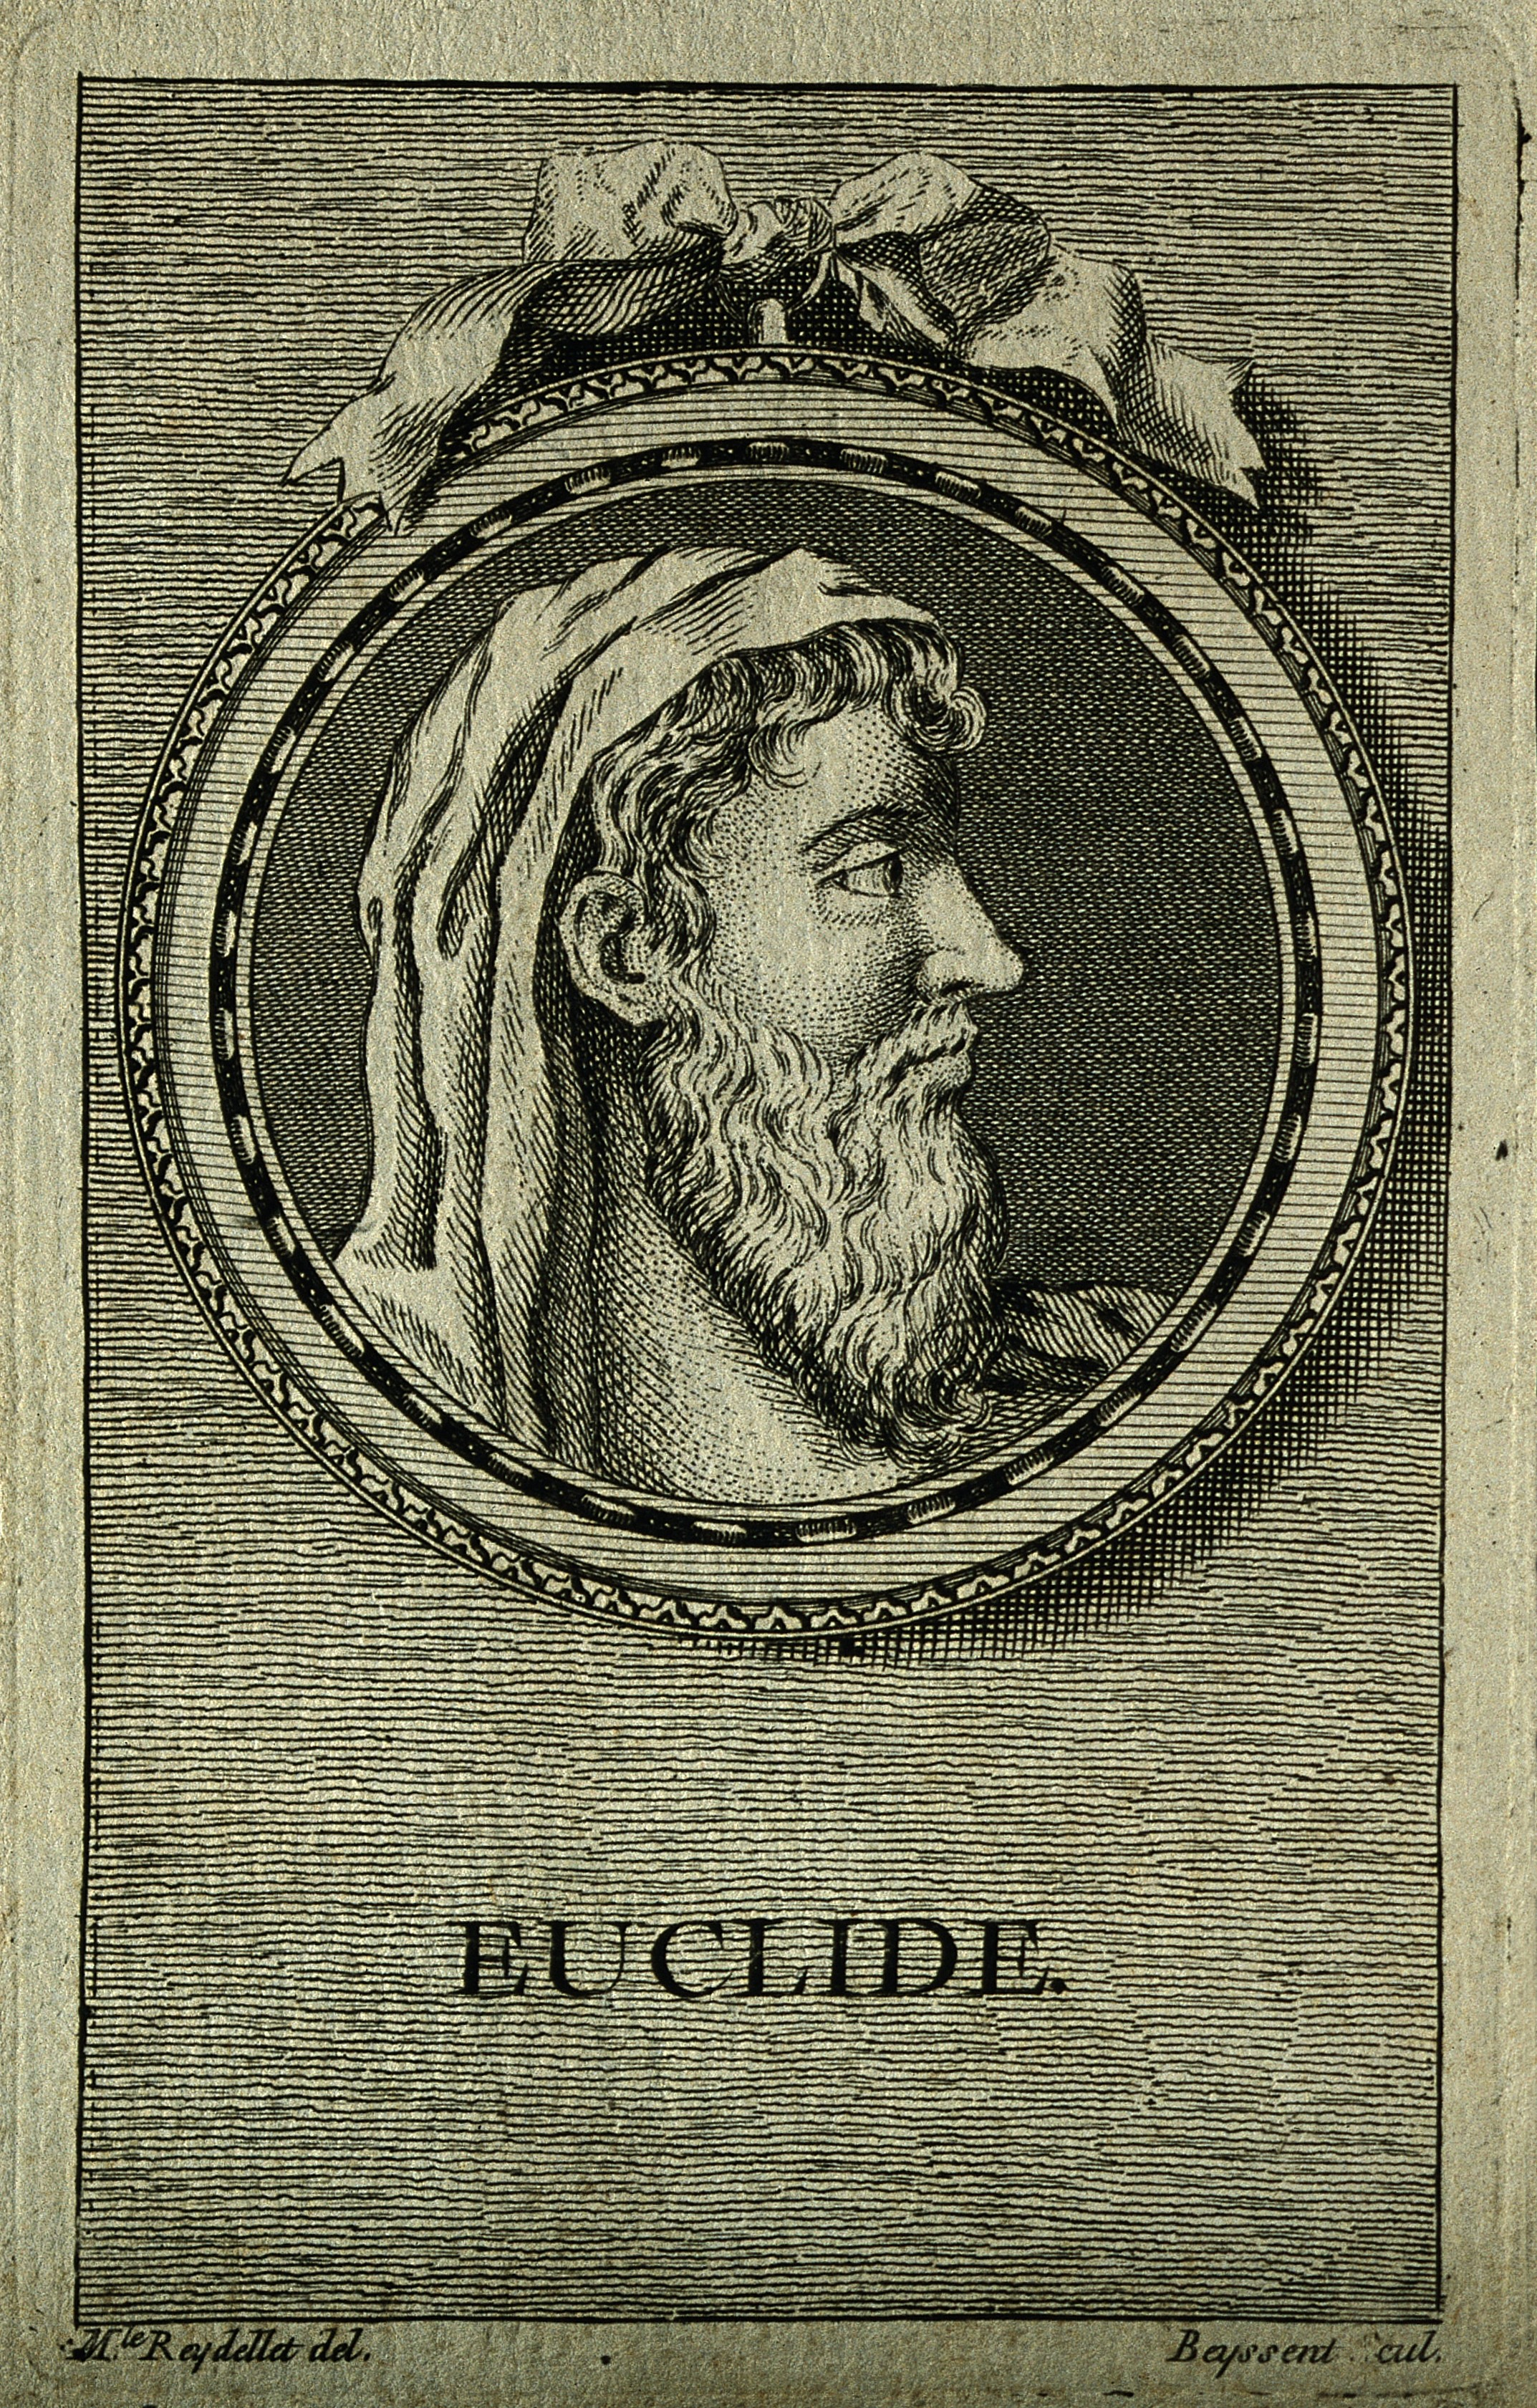
\includegraphics[width=0.3\textwidth]{Euclid-Beyssent-line-engraving.jpg}%
    };
  \end{tikzpicture}
  \caption{Line engraving by S. Beyssent after Mlle. C. Reydell}
  \label{fig:euclid}
\end{wrapfigure}
Number theory has a long history that dates back to antiquity. One of the earliest and most influential systematic treatments of mathematics is Euclid's Elements \cite{euclid1908}, written around 300 BC in Alexandria. In this work, Euclid established several key results in number theory, including the infinitude of primes and the algorithm for finding the greatest common divisor, which bears his name.

Around 250 AD, the Greek mathematician Diophantus of Alexandria wrote his \emph{Arithmetica} \cite{diophantus1910}, which focused on solving what are now known as Diophantine equations. This 13-volume work is often considered the first comprehensive treatment of algebra, though Diophantus relied on rhetorical descriptions rather than modern algebraic notation. Only six of the original volumes have survived, but they profoundly influenced later mathematicians.

The works of Euclid and Diophantus were preserved and studied by scholars in the Byzantine Empire, such as Theon of Alexandria and his daughter Hypatia. They added commentaries that clarified and expanded upon the original text.

During the Islamic Golden Age, scholars like Al-Khwarizmi, Ibn al-Haytham, and Omar Khayyam preserved and expanded upon the works of Euclid and Diophantus. Al-Khwarizmi’s work, especially his \emph{Kitab al-Mukhtasar fi Hisab al-Jabr wal-Muqabala} (from which the term "algebra" originates), introduced systematic methods for solving linear and quadratic equations. He used rhetorical algebra, like Diophantus, but began a transition toward symbolic representation by relying on consistent terminology for operations and equations.

After the invention of the printing press, Erhard Ratdolt, a German printer based in Venice, produced the first printed edition of the Elements in 1482. This edition included mathematical diagrams and marked an important step in the dissemination of Euclid’s work. The first printed edition of Diophantus' Arithmetica was published in 1575 by Wilhelm Xylander, a German mathematician. The printing was done in Basel, Switzerland, a major hub for academic publishing at the time. By the time of Pierre de Fermat in the 17th century, both the Elements and Arithmetica had become essential texts for mathematicians across Europe, influencing the development of number theory and inspiring Fermat’s groundbreaking contributions.

\begin{wrapfigure}[21]{r}{0.4\textwidth}
  \centering
  \begin{tikzpicture}
    \node[inner sep=0pt, rounded corners=0.2em, clip] {%
      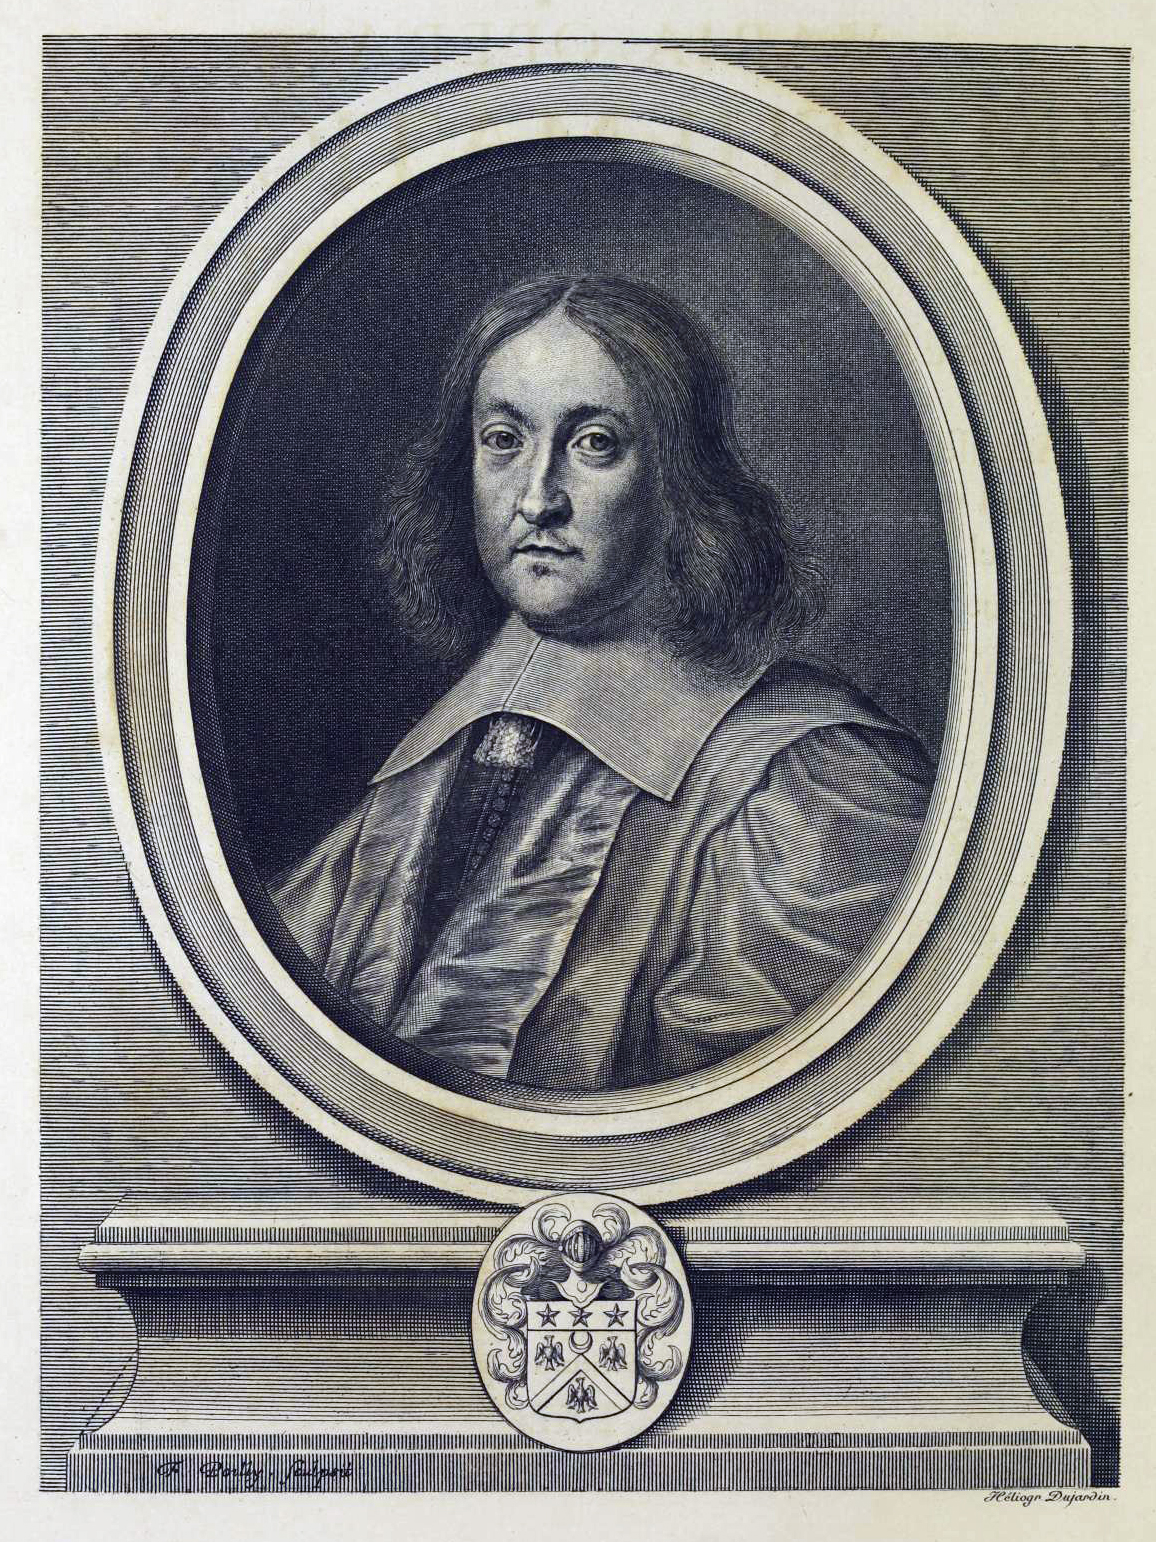
\includegraphics[width=0.38\textwidth]{Fermat.jpg}%
    };
    \end{tikzpicture}
    \caption{Pierre de Fermat. Engraving in Oeuvres Mathématiques Diverses.}
  \label{fig:fermat}
\end{wrapfigure}

Pierre de Fermat (1607–1665) is often considered the founder of modern number theory. He was a contemporary of Blaise Pascal and Marin Mersenne, both of whom he corresponded with, and also of Galileo Galilei. He wrote a manuscript titled \emph{Éléments de Géométrie}, which served as an extension and commentary on Euclid’s Elements. In this work, he sought to modernize Euclid’s geometry by applying the emerging methods of algebra and analytic geometry to classical geometric problems.

Fermat made several groundbreaking contributions to number theory. He proved \emph{Fermat's Little Theorem}, which is a central theorem of this course, and he formulated the \emph{sum of two squares theorem} asserting that an odd prime $p$ can be expressed as the sum of two squares if and only if $p\equiv 1\pmod{4}$. He also introduced the method of \emph{infinite descent}, and formulated the \emph{Polygonal Number Theorem}, which states that every positive integer can be expressed as the sum of at most $n$ $n$-gonal numbers.

Fermat also made several famous conjectures. He conjectured that the equation $x^2+Ny^2=1$ has infinitely many solutions for any non-square integer $N$. Euler made a significant advance to this problem by proving it for specific values of $N$. The general form of the solution to equations of the form $x^2+Ny^2=1$ was found later by Legendre and Lagrange.

Finally, Fermat famously asserted that there could be no three nonzero integers $x$, $y$, and $z$ such that the equation
\begin{equation*}
  x^n+y^n=z^n
\end{equation*}
holds, when $n\geq 3$. This statement is now known as \emph{Fermat's Last Theorem}. He claimed to have a "truly marvelous proof", but that the margin of his copy of \emph{Arithmetica} was too small to contain it. His assertion, known as \emph{Fermat’s Last Theorem}, captivated mathematicians for centuries. It was finally proven in 1995 by Andrew Wiles, about 350 years after Fermat made his famous note in the margin, using advanced techniques from algebraic geometry and modular forms. Wiles’s achievement is considered one of the most remarkable milestones in the history of mathematics.

While Fermat laid the groundwork for modern number theory, we should mention that the concept of \emph{function} hasn't been crystallized until Leibniz coined the term in 1673, using it to describe quantities related to curves, such as slopes, tangents, and areas. Bernoulli played a significant role in expanding the idea of functions. He used the term explicitly in 1718, describing it as a quantity dependent on another variable. Euler provided the first modern definition of a function in his \emph{Introductio in Analysin Infinitorum} (1748) \cite{euler1988}. He emphasized that functions could include both algebraic (e.g., polynomials) and transcendental forms (e.g., trigonometric and exponential functions). Peter Gustav Lejeune Dirichlet was the first to define functions abstractly as a correspondence between two sets, removing the requirement for expressions or formulas. This abstraction was a key insight for the theorem that we now know as \emph{Dirichlet's theorem}: Every arithmetic progression
\begin{equation*}
  a,\ a+b,\ a+2b,\ a+3b,\ \ldots
\end{equation*}
\begin{wrapfigure}[21]{r}{0.4\textwidth}
  \centering
  \begin{tikzpicture}
    \node[inner sep=0pt, rounded corners=0.2em, clip] {%
      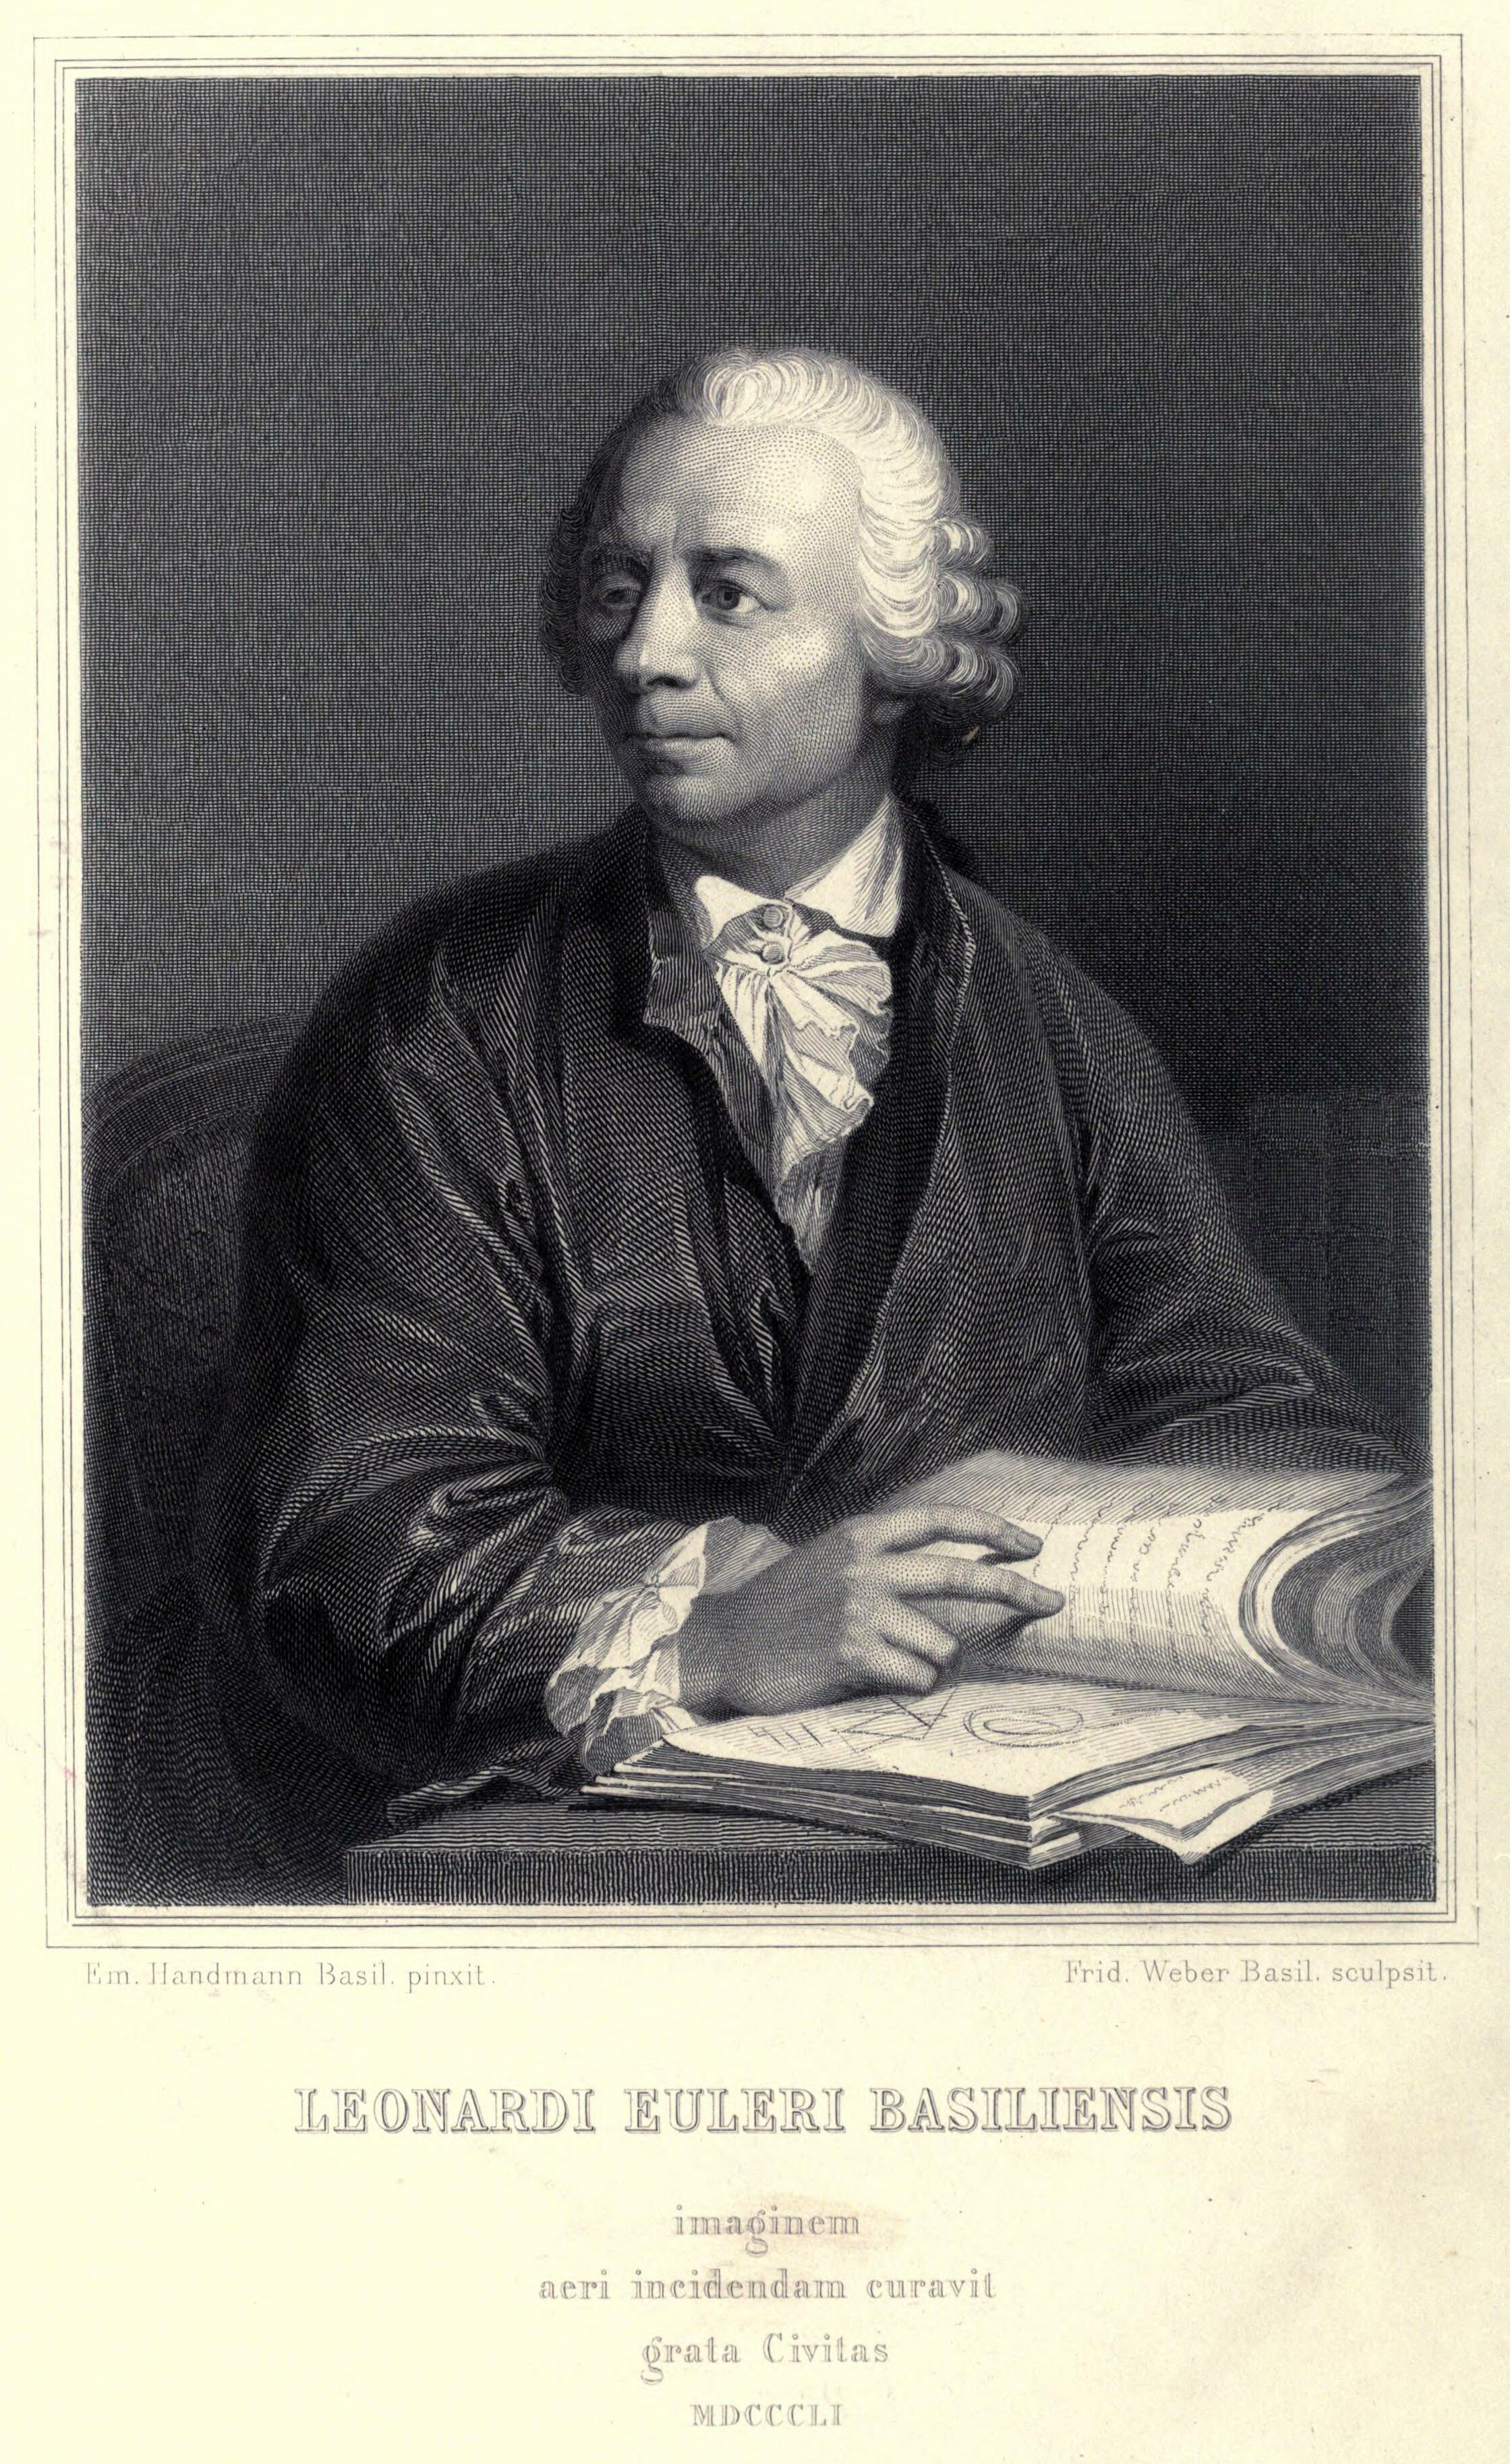
\includegraphics[width=0.38\textwidth]{Euler.jpg}%
    };
  \end{tikzpicture}
  \caption{Leonhard Euler. Engraving by Friedrich Weber.}
  \label{fig:euler}
\end{wrapfigure}
in which $a$ and $b$ are coprime, contains an infinitude of primes. Dirichlet proved his theorem in 1837, more than 150 years after Leibniz first coined the term of function.

Euler's Introductio in Analysin Infinitorum marked the beginning of \emph{analytical number theory}. As we mentioned before, Euler defined functions here and established the notation $f(x)$ of a function applied to its variable, which we still use today. He derived the famous formula for complex exponentials
\begin{equation*}
  e^{ix}=\cos(x) + i \sin(x).
\end{equation*}
This identity connects the exponential function, trigonometric functions, and the imaginary unit. The Riemann zeta function $\zeta(s)$ makes its first appearance here in a complex variable $s$, and he derived the celebrated \emph{product formula}
\begin{equation*}
  \zeta(s)=\sum_{n=1}^{\infty}\frac{1}{n^s}=\prod_{p\,\mathrm{prime}}\frac{1}{1-p^{-s}}.
\end{equation*}
More generally, Euler explored infinite series and products. The \emph{Basel summation formula}
\begin{equation*}
  \sum_{n=1}^\infty \frac{1}{n^2}=\frac{\pi^2}{6}
\end{equation*}
was first proven here, which was one of Euler's most celebrated achievements. Euler was keen to explore the connection between geometry and analysis, and in Introductio in Analysin Infinitorum, he advanced the idea that the study of functions and infinite series could provide new insights into geometric problems. He showed how techniques from analysis could be used to solve problems in geometry and vice versa, fostering the development of applied mathematics.

\begin{wrapfigure}[21]{r}{0.4\textwidth}
  \centering
  \begin{tikzpicture}
    \node[inner sep=0pt, rounded corners=0.2em, clip] {%
      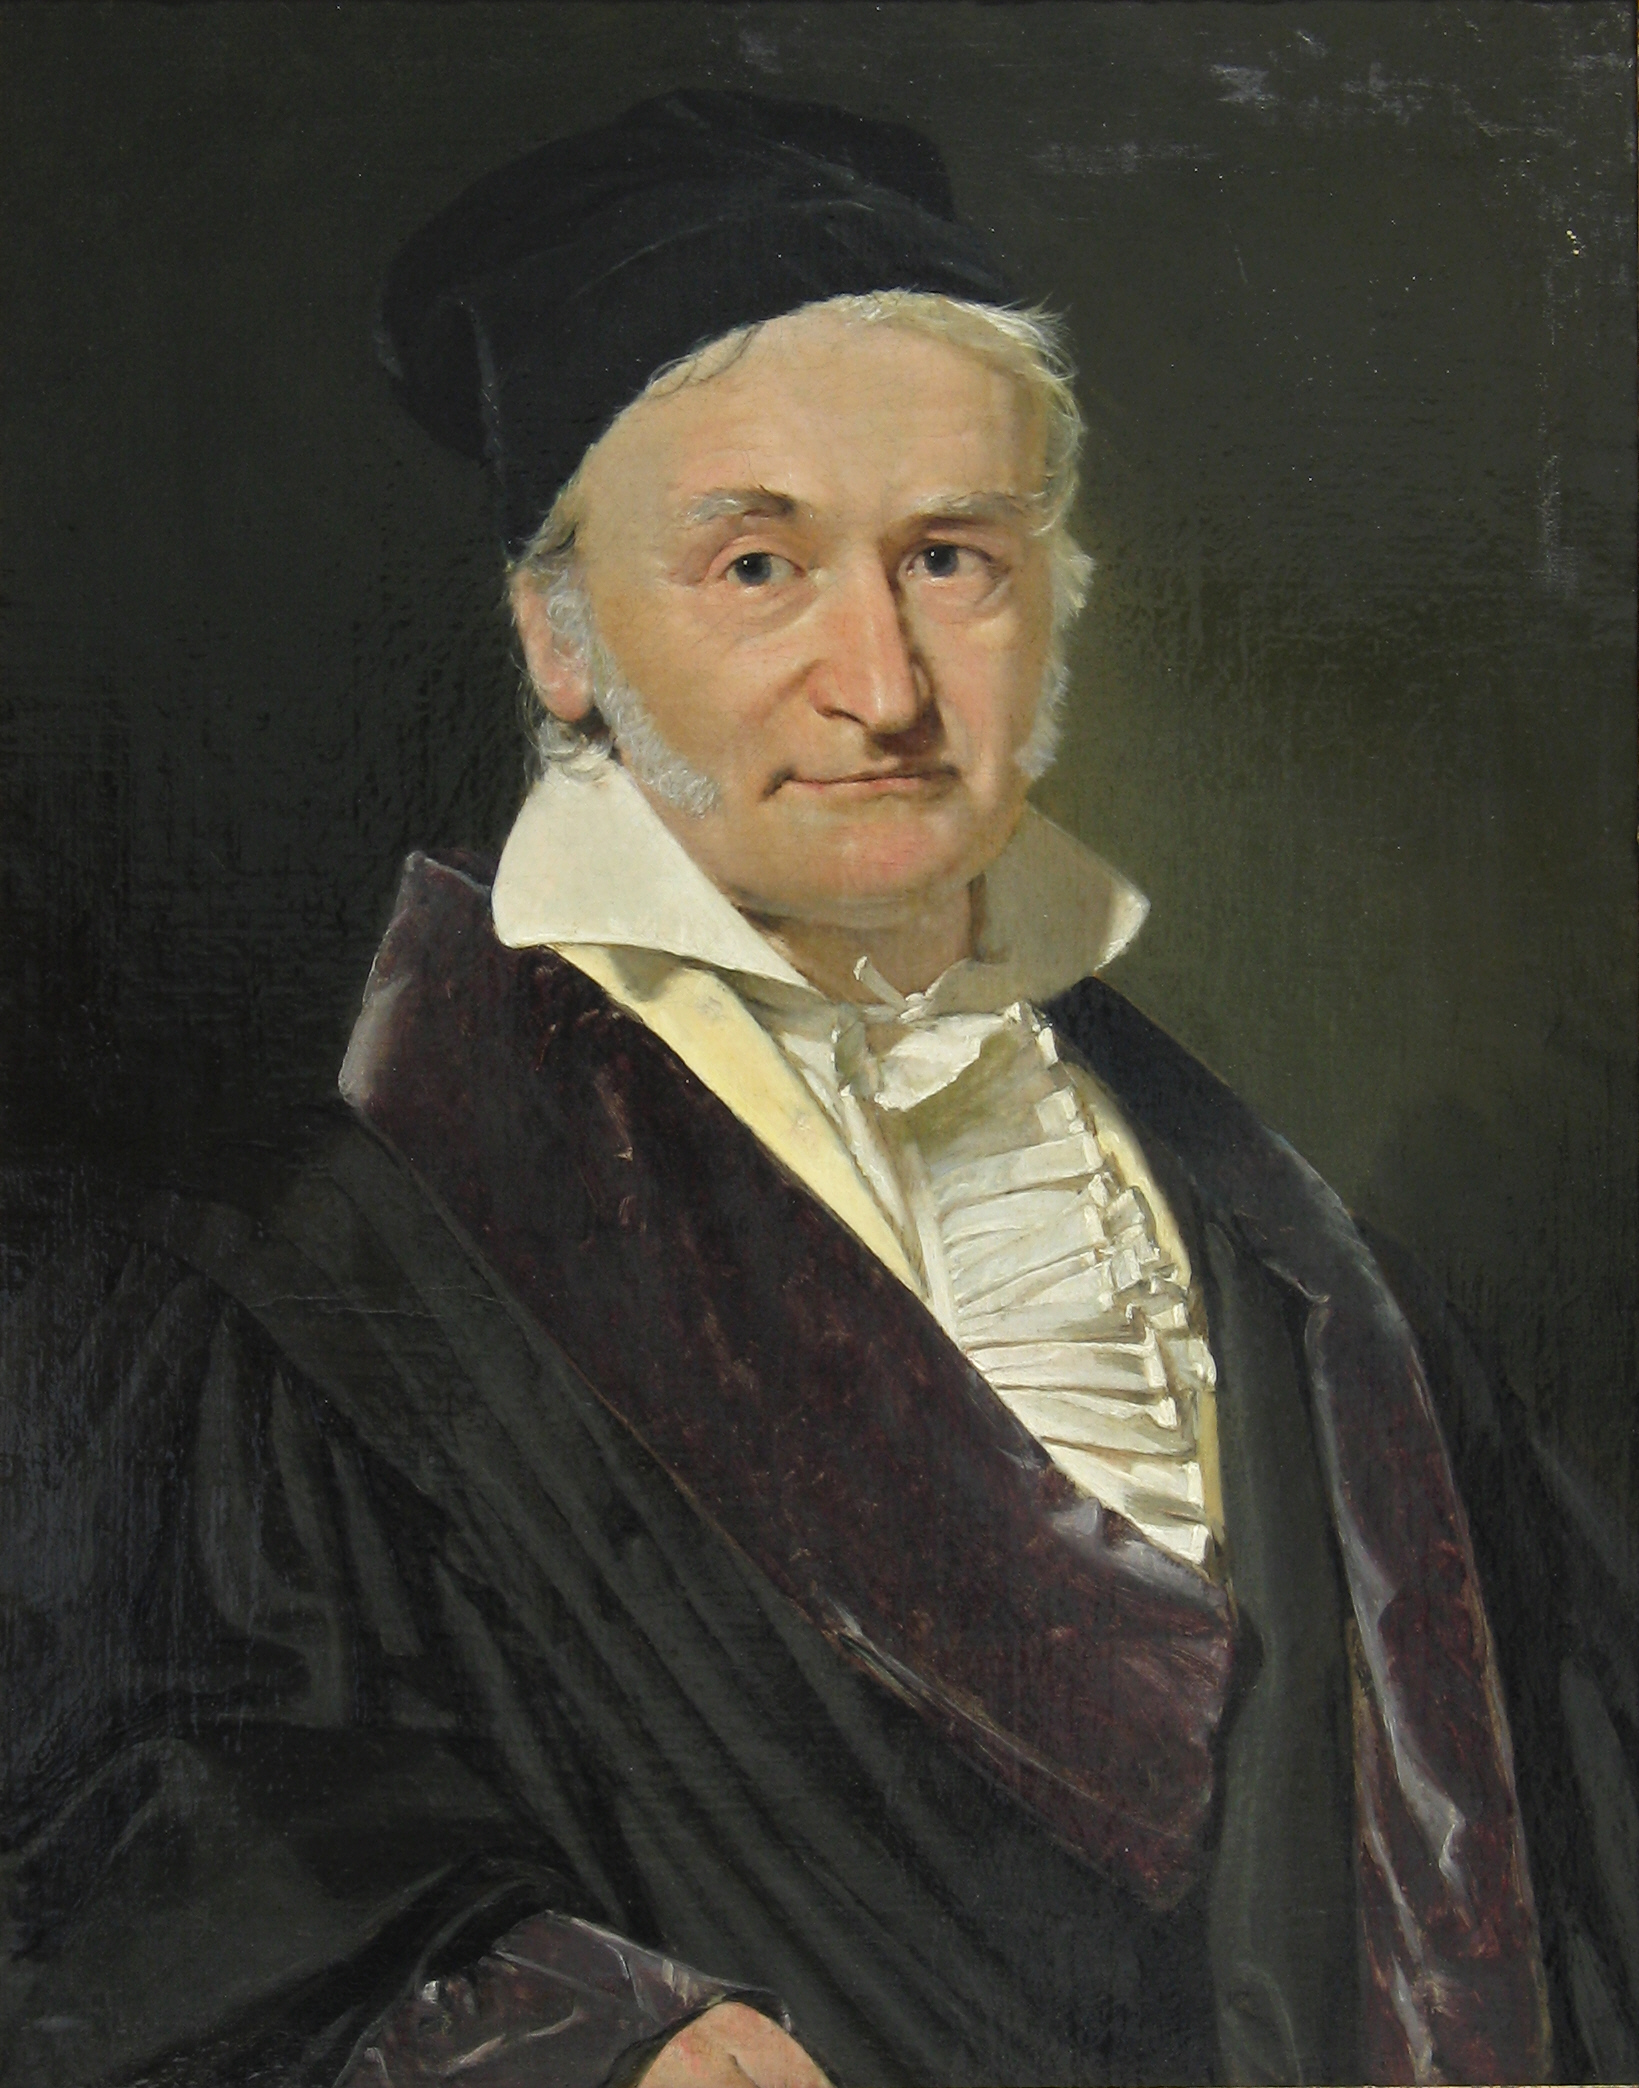
\includegraphics[width=0.38\textwidth]{Gauss.jpg}%
    };
  \end{tikzpicture}
  \caption{\sloppy{Carl Friedrich Gauss. Painting by Christian Albrecht Jensen.}}
  \label{fig:gauss}
\end{wrapfigure}
Building on the work of Euler, Gauss began using the properties of the zeta function and other analytic methods to investigate the distribution of the primes. His seminal work \emph{Disquisitiones Arithmeticae} \cite{gauss1986} is often considered the starting point of the study of the distribution of primes, ultimately leading up to the \emph{Prime Number Theorem}. Gauss conjectured that the number $\pi(n)$ of primes below a number $n$ satisfies the asymptotic law
\begin{equation*}
  \pi(n)\sim\frac{n}{\log(n)}.
\end{equation*}
This conjecture was proved independently by Jacques Hadamard and Charles Jean de la Vallée Poussin. Furthermore, Gauss laid the foundation for modular arithmetic, and proved the celebrated law of quadratic reciprocity, which tells us when a quadratic equation modulo a prime number is solvable. More precisely, it states that if $q\equiv 1\pmod{4}$ then the congruence $x^2\equiv p \pmod{q}$ is solvable if and only if the congruence $x^2\equiv q\pmod{p}$ is solvable.

So far, we have covered some of the most celebrated advances in humanity's understanding of numbers up to the early 19th century. Mathematics has made rapid progress since then. Bertrand's postulate, which asserts that there is always at least one prime $p$ between $n$ and $2n$, for any $n>1$, was proven by Pafnuty Chebyshev in 1852, and Ben Green and Terence Tau proved in 2004 that the sequence of prime numbers contains arbitrarily long arithmetic progressions.

The 20th century saw the emergence of the Langlands program, a far-reaching research program that aims to connect number theory, representation theory, and algebraic geometry. With the contributions of mathematicians like André Weil, Robert Langlands, and many others, the program has shaped much of the direction of modern research in number theory and its applications to other branches of mathematics.

Even today fundamental concepts such as sets and functions continue to evolve. We live in an era of digital computation, with tools far beyond the reach of Fermat, Euler, and Gauss, where essentially all recorded knowledge is readily available to almost anyone. This computational revolution has also given rise to powerful tools like proof assistants—computer programs designed to construct and formally verify mathematical proofs. Since proof assistants are programming languages, they are often based on type theory rather than set theory, slightly changing the way mathematics is done. Functions in type theory are even more general than Leibniz, Euler, and Dirichlet envisioned: unlike in set theory where functions are a specific kind of relations between sets, functions in type theory are primitive entities satisfying certain rules for evaluation, and they have an extra dependency built in, allowing types of their outputs to depend on the input. Proof assistants are being used with great success to formally verify advanced mathematical theorems. Georges Gonthier formally verified the Four Color Theorem and the Odd Order Theorem, and Tom Hales verified Kepler's conjecture about sphere packings. A current effort led by Kevin Buzzard aims to formally verify Fermat's Last Theorem.

Today, number theory continues to be one of the most active and fruitful areas of mathematical research, all of which started simply with counting on ten fingers.

\section*{Overview of the Course}

An integer $a$ is said to \emph{divide} an integer $b$ if there exists an integer $x$ such that $ax=b$. In other words, the number $a$ divides $b$ if the equation
\begin{equation*}
  ax=b  
\end{equation*}
has a solution in the integers. In this case we say that $a$ is a \emph{divisor} of $b$, and we write $a \mid b$. This equation is the simplest example of a Diophantine equation. Diophantine equations are equations expressed using variables, integers, and arithmetic operations. The primary goal of solving a Diophantine equation is to find integers for each of the variables for which the equation is true. The study of Diophantine equations is a cornerstone of number theory.

For example, the equation
\begin{equation*}
  x^2 - 1 = 0
\end{equation*}
is a \emph{quadratic Diophantine equation} with two solutions: $x=\pm 1$. One of the most well-known quadratic Diophantine equations is the equation
\begin{equation*}
  x^2 + y^2 = z^2,
\end{equation*}
which is a Diophantine equation in \emph{three variables}. Its solutions are known as \emph{Pythagorean triples}. These triples, such as $(3,4,5)$ and $(5,12,13)$, corresponds to the side lengths of right-angled triangles and have been studied since antiquity. Perhaps the most famous Diophantine equation is Fermat's equation
\begin{equation*}
  x^n + y^n = z^n,
\end{equation*}
which has no solutions for nonzero integers $x$, $y$, and $z$ when $n\geq 3$.

In this course, however, we will not go as far as proving Fermat's last theorem. The first target of this course is the Fundamental Theorem of Arithmetic, which establishes the prime numbers as the building blocks of all natural numbers. A number $n$ is said to be prime if it has exactly one divisor $d \mid n$ such that $d\neq n$. If this is the case, then its unique divisor that is not equal to itself is the number $1$. The Fundamental Theorem of Arithmetic asserts that any nonzero natural number $n$ can be written as a product of primes
\begin{equation*}
  n=p_1p_2\cdots p_k,
\end{equation*}
and that this decomposition of $n$ as a product of primes is unique up to the ordering of the primes.

In order to study divisibility properties more deeply, Gauss introduced in his \emph{Disquisitiones Arithmeticae} the congruence relations of modular arithmetic. Following Gauss, we say that a number $a$ is congruent to $b$ modulo $n$, that is,
\begin{equation*}
  a \equiv b \pmod{n}
\end{equation*}
if $n \mid b - a$. Gauss used this new formalism to study quadratic residues, the Chinese Remainder theorem, and a variety of other problems in number theory, a thread we will also pick up on in this course.

Some of the most important theorems in this context are Fermat's Little Theorem, Euler's Theorem, and Wilson's Theorem. Fermat's theorem asserts that given any prime number $p$ and any number $a$ that is not divisible by $p$ we have
\begin{equation*}
  a^{p-1}\equiv 1 \pmod{p}.
\end{equation*}
Fermat's theorem is an important ingredient in primality tests: If the congruence $a^{n-1}\equiv 1 \pmod{n}$ is false then the number $n$ cannot be prime. Testing this congruence for several values of $a$ is a simple way of discovering that $n$ is composite. This test is by itself, however, not conclusive because there are some numbers, the Carmichael numbers, that satisfy Fermat's congruence for all $a$ relatively prime to $n$.

Euler's theorem is a sharper version of Fermat's Little Theorem, but it involves a new function: \emph{Euler's totient function}. Euler's totient function $\phi$ counts the numbers less than $n$ that are relatively prime to $n$, which means that they share no common divisors with $n$ other than $1$. For example, if $p$ is a prime number then $\phi(p)=p-1$ since every number $0<n<p$ is relatively prime to $p$. Using the totient function, Euler's theorem asserts that the congruence relation
\begin{equation*}
  a^{\phi(n)}\equiv 1 \pmod{n}
\end{equation*}
holds for any natural number $n$ and any number $a$ relatively prime to $n$. Euler's theorem has applications in cryptography.

Wilson's Theorem states that a number $p$ is a prime number if and only if the congruence
\begin{equation*}
  (p-1)!\equiv -1 \pmod{p}
\end{equation*}
holds. Here, the exclamation mark is used for the \emph{factorial function}: The number $n!$ is the product $1\cdots n$ of all the numbers from $1$ through $n$. Wilson's Theorem therefore gives another criterion for primality testing.

Euler's totient function is an example of an arithmetic function. Other such functions include the function $\tau(n)$, which returns the number of divisors of a number $n$, the function $\sigma(n)$, which returns the sum of the divisors of a number $n$, and the \emph{M\"obius function} $\mu$. These and other functions have important relations between them, that we will investigate next. The M\"obius inversion formula, for instance, states that if $f$ and $g$ are two arithmetic functions, then we have
\begin{equation*}
  f(n)=\sum_{d\mid n} g(d)\qquad\text{if and only if}\qquad g(n)=\sum_{d\mid n}\mu(d)f\left(\frac{n}{d}\right).
\end{equation*}
This result allows us to "invert" summation relations involving divisors.

The M\"obius inversion is only one aspect of an algebraic structure that is present on the set of all arithmetic functions. Arithmetic functions can be multiplied by an operation known as \emph{Dirichlet convolution}, which gives the set of arithmetic functions the structure of a \emph{commutative ring}. Commutative rings are sets with operations of addition and multiplication satisfying the usual laws of arithmetic, and having such a structure on a set gives us a great opportunity to study them further. In our case, we get to study the primes more closely.

Experimentation is essential in number theory. By making lists of primes, lists of numbers that can be written as the sum of two squares or sums of three squares, lists of square-free numbers, and so on, you will start to gather data on numbers and perhaps start seeing patterns that might otherwise feel elusive. At the end of this section, we have produced two number grids with the numbers from $1$ to $1728$. The great masters all have endlessly created such lists to organize and discover patterns in various kinds of numbers. Feel free to print it as many times as you like, and color them according to your own rules, or whenever something in the course piques your interest. Some exercises throughout the course will ask you to color this number grid in a certain way.

\section*{Literature}
In this course we will be following \cite{andrews1994} fairly closely. One distinctive feature of this book is that it presents many of the most important theorems from two perspectives: a combinatorial one and an abstract one. This dual approach helps to clarify not only why these results are true but also appreciate why they are natural and inevitable within the broader framework of mathematics.

However, there are many excellent sources to learn number theory from. One of my personal favorites for its clarity and accessibility is LeVeque's \emph{Topics in Number Theory} \cite{leveque1956vol1,leveque1956vol2}. Both Andrews' and LeVeque's textbooks contain plenty of exercises, most of which are very fun.

Silverman's \emph{Friendly Introduction to Number Theory} \cite{silverman2012} is another wonderful textbook, explaining the ideas behind many theorems and methods in number theory in a very accessible way, with practical examples and exercises. If you find some parts of Andrews or these notes hard to follow, you may well find the Friendly Introduction very helpful.

The undisputed classic textbook on number theory is Hardy and Wright's \emph{Introduction to the Theory of Numbers} \cite{hardy2008}. This book covers all the essential topics in number theory, including elementary number theory and analytical number theory. It is more comprehensive and also provides more historical notes. The textbook of Hardy and Wright does not provide exercises, but it contains the proofs of many important facts in number theory that are stated as exercises elsewhere.

\section{Online resources}

There are plenty of ways to learn number theory and engage with communities of mathematicians and students online. First and foremost, wikipedia has many excellent pages on topics from and related to number theory. The website math.stackexchange.com is dedicated to answering any kind of mathematical questions, although the more research related questions are usually posed on mathoverflow.net. The website artofproblemsolving.com is dedicated to contest mathematics and the problem solving techniques necessary to do well in competitions such as the International Mathematics Olympiad. Furthermore, there are some popular channels on video sharing sites such as YouTube and TikTok. We mention some of the most popular channels:

Lectures:
\begin{enumerate}
\item Richard Borcherds is a Fields Medalist, and has recorded many of his Berkeley lectures for YouTube. This is a must-watch.
\end{enumerate}

Problem solving:
\begin{enumerate}
\item \textbf{Michael Penn} has an excellent YouTube channel in which he solves interesting mathematical problems on a blackboard, at roughly the level of this course.
\item vEnhance (Evan Chen) is an IMO gold medalist and author of the book \emph{Euclidean Geometry in Math Olympiads} \cite{chen2016}. He streams live solves of olympiand math problems on Twitch and his videos are also available on youtube.\item OmegaLearn is Jonathan Huang's YouTube channel about solving IMO problems. Some of his playlists dive deeper into specific techniques such as Fermat's infinite descent.
\item MindYourDecisions (Presh Talwalkar) presents puzzles and number-theoretic tricks, often with surprising or elegant solutions.
\item Math with Ms. Lin
\item Sokoban’s Den
\item Brent Ferguson’s Math
\end{enumerate}

Mathematics for a broad audience:
\begin{enumerate}
\item \textbf{3Blue1Brown} dives deeply into a variety of topics related to computer science and mathematics with compelling visualizations
\item Mathologer is Burkard Polster's YouTube channel for recreative mathematicians. Many of his videos contain nice visual proofs, especially his videos about Fermat's Two-Square theorem and the quadratic reciprocity theorem are worth watching.
\item Numberphile is a long running YouTube channel of Brady Haran in which mathematicians are interviewed to explain a variety of mathematical phenomena, includin topics related to number theory.
\item Standupmaths
\item Blackpenredpen
\item Tom Rocks Maths
\item @professorpuzzle (TikTok)
\item @numeracynerd (TikTok)
\end{enumerate}

You might also enjoy joining some Discord servers, such as the AoPS community server (Art of problem solving), the Math Stack Exchange Discord, or the OmegaLearn Server.

Finally, you might also find generative AI useful in exploring mathematical topics, such as ChatGPT! These are useful, because you can ask them to explain any topic that interests you, and their answers are quickly getting better. Be careful, however, to always make sure you understand an answer for yourself, because their reasoning is not always on point.

\afterpage{%
  \pagestyle{empty}
  \clearpage
  \begin{figure*}[p]
    \centering
    \resizebox{\textwidth}{!}{%
      \begin{tikzpicture}[x=0.5cm,y=0.5cm]
        
        % PARAMETERS
        \def\Cols{24}                       % number of columns
        \def\N{864}                        % max number
        \pgfmathsetmacro{\Rows}{ceil(\N/\Cols)}  % computed number of rows
        \def\CirDiam{0.4cm}                 % diameter of every circle
        
        % 1) draw every number in a white circle of fixed size
        \foreach \i in {1,...,\N} {
          \pgfmathtruncatemacro{\c}{mod(\i-1,\Cols)}
          \pgfmathtruncatemacro{\r}{int((\i-1)/\Cols)}
          \node[
          circle,
          draw,
          fill=white,
          minimum size=\CirDiam,
          inner sep=0pt,
          font=\tiny
          ] at (\c+0.5,-\r-0.5) {\i};
        }
        
      \end{tikzpicture}%
    }
  \end{figure*}
  \begin{figure*}[p]
    \centering
    \resizebox{\textwidth}{!}{%
      \begin{tikzpicture}[x=0.5cm,y=0.5cm]
        
        % PARAMETERS
        \def\Cols{24}                       % number of columns
        \def\N{864}                        % max number
        \pgfmathsetmacro{\Rows}{ceil(\N/\Cols)}  % computed number of rows
        \def\CirDiam{0.4cm}                 % diameter of every circle
        
        % 1) draw every number in a white circle of fixed size
        \foreach \i in {1,...,\N} {
          \pgfmathtruncatemacro{\c}{mod(\i-1,\Cols)}
          \pgfmathtruncatemacro{\r}{int((\i-1)/\Cols)}
          \pgfmathtruncatemacro{\v}{\N+\i}
          \node[
          circle,
          draw,
          fill=white,
          minimum size=\CirDiam,
          inner sep=0pt,
          font=\tiny
          ] at (\c+0.5,-\r-0.5) {\v};
        }
        
      \end{tikzpicture}%
    }
  \end{figure*}
  \clearpage
}

%%% Local Variables:
%%% mode: latex
%%% TeX-master: "elementary-number-theory"
%%% End:


\mainmatter

\part{The Nature of Numbers}

\chapter{The Nature of Numbers}\label{chapter:induction}

\section{On the Concept of Number Throughout History}

Many people are familiar with numbers through everyday experiences like counting, measuring, or comparing quantities. From a young age, we develop an intuition about how numbers behave. Our experience with numbers reveals patterns of truths and properties that seem to always be true. For example, we quickly learn that it does not matter in which order we add two numbers: Given two numbers $a$ and $b$ it is always true that $a+b=b+a$. Truths such as this one seem so self-evident that we might be tempted to just accept them. However, for a rigorous mathematical theory we need to be more careful. Mathematicians require proofs—conclusive arguments that establish why certain properties hold universally for all numbers, or at least for precisely defined sets of numbers. Checking a property for every number up to a hundred, a million, or even $10^{27}$ might confirm a pattern, but infinitely many numbers remain beyond such finite checks. To reason about all natural numbers at once, we need formal principles that extend beyond empirical observation and anecdotal evidence. In order to discover such reasoning principles, we need to find out what the natural numbers really are.

Although natural numbers arise from counting, the notion of number is not inherently linked to any particular collection of entities being counted. Scholars in the Pythagorean tradition were among the first to articulate this insight. Nicomachus emphasized the concepts of \emph{monad}, \emph{dyad}, and \emph{triad} for the totality of all things that come in one, two, or three units \cite{nicomachus1926}. Nicomachus ascribed divine properties to the monad, or unity: ``{\it It generates itself without beginning, without end, and appears to be the cause of enduring, as God in the realm of physical actualities is in such manner perceived of as a preserving and guarding agent of nature}''. Nicomachus drew strong parallels between the monad and the concept of sameness, and likewise between the dyad and the concept of otherness. He also emphasized that numbers were composed of monads. In other words, the monad is the source of all numbers. Although mathematicians do not ascribe divine properties to numbers anymore, we see here the emergence of some important ideas. The first is that all numbers are generated from the monad, that is, unity. The second idea is to connect unity with sameness. The idea that all things equal to a given object form a unit, or a singleton, anticipates a fundamental principle of equality. However, we shall forego the interesting digressions that we could make about equality and focus our attention on the concept of number.

With Euclid, we see a shift away from the divine conception of the monad. For Euclid, a \emph{unit} is the conceptual principle by which an individual object is identified as one, and a \emph{number} is a multitude composed of such units in a discrete fashion \cite{euclid2015}. In other words, the concept of unit captures the notion of oneness, but this is distinct of the number $1$ itself. Both Nicomachus's and Euclid's views on the concept of number were highly influential throughout late antiquity and the Middle Ages, particularly through Boethius's Latin rendition of Nicomachus's \emph{Introduction to Arithmetic} and Adelard of Bath's translation of Euclid's \emph{Elements}.

While Pierre de Fermat is regarded the founder of modern number theory, he did not write extensively on the philosophy of mathematics. Nevertheless, certain themes in his correspondence and work show a clear orientation. For him, mathematics is about truths intrinsic to numbers. Numbers were the object of exact reasoning. He emphasized that \emph{induction}, by which mathematicians up to the early 19th century understood experimental verification, was insufficient to establish universal truths of numbers. Among Fermat’s lasting contributions was his method of infinite descent, a method of proof by contradiction in which one shows that any supposed solution would lead to an ever-decreasing sequence of natural numbers, which is impossible.

With Euler, we witness a significant conceptual expansion. In his \emph{Elements of Algebra}, Euler extended the notion of number beyond the natural and rational to encompass negative numbers, irrationals, complex numbers, and even infinite series. He was among the first to conjecture that constants like $e$ and $\pi$ are transcendental; that is, not the roots of any algebraic equation with rational coefficients. For Euler, numbers were entities governed by formal laws, irrespective of whether they corresponded to geometric magnitudes. Euler's broadening of the concept of numbers, and his use of analytic methods would eventually spark debates about the foundations of mathematics and the logical principles underlying mathematical truth.

In the 19th century, the nature of mathematics itself began to change. The emergence of non-Euclidean geometry was a challenge to the status of Euclid's Elements as the de facto foundation of mathematics. Weierstrass's discovery of continuous, nowhere differentiable functions underscored the need for a more solid foundation of calculus, and with Galois's use of symmetries in order to show that quintic equations had no solutions expressible in terms of radicals abstract algebra started to become more prominent.

We view the set of numbers as an abstract entity that exist as a precisely specified concept within the collective imagination of conscious beings to convey and communicate ideas such as counting, comparing, and measuring quantities.

When we say that the natural numbers are the numbers $0$, $1$, $2$, $\ldots$, we really mean that the natural numbers are generated from $0$ and the \define{successor function} $n\mapsto n+1$. The collection of all natural numbers forms a set or type

\begin{equation}
  \mathbb{N}:=\{0,1,2,\ldots\}.
\end{equation}

Mathematicians often prefer to work with sets, while computer scientists might prefer to work with types, both of which are collections of abstract objects often referred to as \define{elements}. The distinction is merely that of the logical framework being used: Most mathematicians rely on the Zermelo--Fraenkel set theory, while computer scientist rely on programming languages that often have a type theory in its foundation. Theorem proving in computer programs called \emph{proof assistants} is rapidly becoming a more essential mathematical activity for students and researchers alike. However, many of the most popular proof assistants are based on type theory, in which collections of mathematical objects are called types.

\section{Induction and Recursion}

The natural number zero and the successor function together are sufficient to describe all the natural numbers. The mathematician's way to express this sufficiency is by stating the principle of \define{mathematical induction}: Given any property $P(n)$ expressing a condition of an arbitrary natural number $n$, in order to prove that $P(n)$ is true for all $n$ it suffices to prove that:
\begin{enumerate}
\item The property $P(0)$ is true.
\item For all $n$, if the property $P(n)$ holds then the property $P(n+1)$ holds.
\end{enumerate}
Mathematical induction works, because every natural number is either $0$ or it is the successor of a previous natural number. Proving a property for all natural numbers therefore breaks down in two cases: The \define{base case} in which we prove that $P(0)$ is true, and the \define{inductive step} where we prove that $P(n+1)$ is true provided that $P(n)$ is true.

Proofs by induction can be broken down into the following steps: First identify the property $P(n)$ that you want to prove by induction. The goal of an induction proof is to prove that $P(n)$ is true for all $n$. Then prove the base case. While this step is often trivial, it is a necessary and essential part of an induction proof. Finally, for the inductive step, write down the exact induction hypothesis, namely the property $P(n)$, and the exact goal of the inductive step, namely the property $P(n+1)$. Then use the induction hypothesis to prove that $P(n+1)$ then also holds. After these steps the proof that $P(n)$ holds is complete.

Since we have previously defined the set of natural numbers to be a set equipped with an element $0$ and a function $S$, satisfying an induction principle, it is of some importance to demonstrate that this definition is sufficiently strong to define familiar operations on the natural numbers, such as addition and multiplication, and to verify their laws.

This naturally leads us to the principle of \define{recursion}, which allows us to define certain operation by a mechanism that is not unlike induction. While the induction principle of the natural numbers is used to \emph{prove} properties uniformly about the natural numbers, recursion is a way to \emph{define} functions, operations, and sequences of elements. Its general principle is that if we wish to specify a function $f:\mathbb{N}\to X$ by recursion, then we have to specify its value at $0$ and its value at $n+1$ using an expression that possibly refers to $n$ and the value $f(n)$. More precisely, a function $f$ is defined by recursion as follows:
\begin{align*}
  f(0) & := x_0 \\
  f(n+1) & := h(n,f(n)).
\end{align*}
Here $h$ is a function that is previously defined. If we define $f$ in this way, then by definition $f$ satisfies the equalities
\begin{align*}
  f(0) & = x_0 \\
  f(n+1) & = h(n,f(n)).
\end{align*}

An important special case of recursion, by which we will define many examples of recursive functions, is to iterate any function $f$ on any set $X$: We define the $n$th iteration $f^n$ of $f$ by
\begin{align*}
  f^0(x) & := x \\
  f^{n+1}(x) & := f(f^n(x)). 
\end{align*}
In other words, the $0$th iteration of $f$ is the \define{identity function}, which leaves all elements untouched, and the $(n+1)$st iteration of $f$ is obtained by applying $f$ once more to the values of the $n$th iteration of $f$.

Notice that we made a choice in the definition of the $(n+1)$st iteration of $f$. We could have defined it alternatively by $f^{n+1}(x):=f^n(f(x))$. In the following proposition we will prove by induction that this leads to the same definition.

\begin{proposition}\label{proposition:iterate-successor}
  Consider a function $f:X\to X$ on a set $X$, and let $n$ be a natural number. Then we have
  \begin{equation*}
    f^{n+1}(x) = f^n(f(x))
  \end{equation*}
  for all $x\in X$.
\end{proposition}

\begin{proof}
  The proof is by induction on $n$. In the base case, we must show that
  \begin{equation*}
    f^1(x) = f^0(f(x)).
  \end{equation*}
  By our definition of $f^n(x)$, we have that $f^1(x)=f(f^0(x))$, and we have $f^0(x)=x$, so that
  \begin{equation*}
    f^1(x)=f(f^0(x))=f(x)=f^0(f(x)).
  \end{equation*}
  This proves the base case. In the inductive step, we assume as our inductive hypothesis that
  \begin{equation*}
    f^{n+1}(x)=f^n(f(x))
  \end{equation*}
  for every $x\in X$. Our goal is then to show that
  \begin{equation*}
    f^{n+2}(x)=f^{n+1}(f(x)).
  \end{equation*}
  Here we use that $f^{n+1}(y)=f(f^n(y))$ for all $y\in X$. Indeed, this allows us to complete the proof:
  \begin{equation*}
    f^{n+2}(x) = f(f^{n+1}(x)) = f(f^n(f(x)))=f^{n+1}(f(x)).\qedhere
  \end{equation*}
\end{proof}

\section{Addition of Natural Numbers}

\begin{definition}
  The \define{addition operation} ${+}:\mathbb{N}\to\mathbb{N}\to\mathbb{N}$ is a binary operation defined by iterating the successor function $S$:
  \begin{equation*}
    m+n := S^n(m).
  \end{equation*}
  In other words, $m+n$ is the $n$th successor of $m$.
\end{definition}

The operation $m,n\mapsto m+n$ satisfies the equalities
\begin{align*}
  m+0 & = m \\
  m+(n+1) & = (m+n)+1
\end{align*}
by definition. However, the equalities
\begin{align*}
  0+n & = n \\
  (m+1)+n & = (m+n)+1
\end{align*}
require a short proof.

\begin{proposition}\label{proposition:unit-law-addition-nat}
  For any two natural numbers $m$ and $n$ we have
  \begin{align*}
    0+n & = n \\
    (m+1)+n & = (m+n)+1.
  \end{align*}
\end{proposition}

\begin{proof}
  The proof of both equalities is by induction on $n$. For the base case of the first equality, note that the equality $0+0=0$ holds by definition. For the inductive step, assume that $0+n=n$. Then we have
  \begin{equation*}
    0+(n+1)=(0+n)+1= n+1.
  \end{equation*}
  For the base case of the second equality, note that the equalities $(m+1)+0=m+1=(m+0)+1$ hold by definition. For the inductive step, assume that $(m+1)+n=(m+n)+1$. Then we have
  \begin{equation*}
    (m+1)+(n+1)=((m+1)+n)+1=((m+n)+1)+1=(m+(n+1))+1.\qedhere
  \end{equation*}
\end{proof}

\begin{proposition}\label{proposition:iterate-add}
  For any function $f:X\to X$, we have
  \begin{equation*}
    f^{m+n}(x)=f^m(f^n(x)).
  \end{equation*}
\end{proposition}

\begin{proof}
  The proof is by induction on $n$. In the base case, we have $m+0=m$ and $f^0(x)=x$. Together, these identities give:
  \begin{equation*}
    f^{m+0}(x)=f^m(x)=f^m(f^0(x)).
  \end{equation*}
  For the inductive step, assume that for every element $x\in X$ we have $f^{m+n}(x)=f^m(f^n(x))$. Our goal is to show that
  \begin{equation*}
    f^{m+(n+1)}(x)=f^m(f^{n+1}(x)).
  \end{equation*}
  Here, we use that $m+(n+1)=(m+n)+1$ and that $f^{n+1}(x)=f(f^n(x))$ hold by definition, and that $f^m(f(x))=f(f^m(x))$ by \cref{proposition:iterate-successor}. Together, these identities give:
  \begin{equation*}
    \begin{split}
      f^{m+(n+1)}(x)=f^{(m+n)+1}(x) & =f(f^{m+n}(x))=f(f^m(f^n(x))) \\
                                    & =f^m(f(f^n(x)))=f^m(f^{n+1}(x)).\qedhere
    \end{split}
  \end{equation*}
\end{proof}

\begin{corollary}
  Addition of natural numbers is \define{associative}: For any three natural numbers $l$, $m$, and $n$ we have
  \begin{equation*}
    (l+m)+n = l+(m+n).
  \end{equation*}
\end{corollary}

\begin{proof}
  By definition, we have $(l+m)+n=S^n(S^m(l))$ and $l+(m+n)=S^{m+n}(l)$. Combining these identities with \cref{proposition:iterate-add}, we obtain
  \begin{equation*}
    (l+m)+n=S^n(S^m(l))=S^{m+n}(l)=l+(m+n).\qedhere
  \end{equation*}
\end{proof}

\begin{proposition}
  Addition of natural numbers is \define{commutative}: For any two natural numbers $m$ and $n$, we have
  \begin{equation*}
    m+n=n+m.
  \end{equation*}
\end{proposition}

\begin{proof}
  The proof is by induction on $n$. In the base case, we use \cref{proposition:unit-law-addition-nat}
  \begin{equation*}
    m+0=m=0+m.
  \end{equation*}
  For the inductive step, assume that $m+n=n+m$. Then we use \cref{proposition:unit-law-addition-nat} again to obtain:
  \begin{align*}
    m+(n+1) & = (m+n)+1 \\
            & = (n+m)+1 \\
            & = (n+1)+m.\qedhere
  \end{align*}
\end{proof}

Some further useful identifications of addition, which follow from the associativity and commutativity laws, are:
\begin{align*}
  (l+m)+n & = (l+n)+m \\
  l+(m+n) & = m+(l+n) \\
  (k+l)+(m+n) & = (k+m)+(l+n).
\end{align*}
The last identification is called the \define{interchange law} for addition. The first one follows from the second, and the second and third are proven by a short calculation:
\begin{align*}
  l+(m+n) & = (l+m)+n & (k+l)+(m+n) & = k+(l+(m+n)) \\
          & = (m+l)+n & & = k + (m + (l+n)) \\
          & = m+(l+n) & & = (k+m)+(l+n).
\end{align*}

\section{Arithmetic of Natural Numbers}

\begin{definition}
  The multiplication function $m,n\mapsto mn$ on the natural numbers is defined recursively by
  \begin{align*}
    m0 & := 0 \\
    m(n+1) & := mn + m.
  \end{align*}
\end{definition}

\begin{proposition}
  Multiplication of natural numbers satisfies the following laws:
  \begin{align*}
    0n & = 0 & m0 & = 0 \\
    (m+1)n & = mn+n & m(n+1) & = mn+m \\
    1m & = m & m1 & = m \\
    l(m+n) & = lm+ln & (l+m)n & = ln+mn \\
    (lm)n & = l(mn) & mn & = nm.
  \end{align*}
\end{proposition}

\begin{proof}
  We prove that $0n=0$ by induction on $n$. In the base case, we have the equality $00=0$. For the inductive step, assume that $0n=0$. Then $0(n+1)=0n+0=0n=0$, completing the proof of the first identity. The identity $m0=0$ holds by definition.

  The proof that $(m+1)n=mn+n$ is again by induction on $n$. In the base case, we have the equalities $(m+1)0=0=m0=m0+0$. For the inductive step, assume that $(m+1)n=mn+n$. Then we have
  \begin{equation*}
    (m+1)(n+1)=(m+1)n+(m+1)=(mn+n)+(m+1)=(mn+m)+(n+1)=m(n+1)+(n+1).
  \end{equation*}
  The identity $m(n+1)=mn+m$ holds by definition.

  Next, we prove first that $mn=nm$, by induction on $n$. In the base case, we have the equalities $m0=0=0m$. For the inductive step, assume that $mn=nm$. Then we have that
  \begin{equation*}
    m(n+1)=mn+m=nm+m=(n+1)m.
  \end{equation*}

  Now we prove that $l(m+n)=lm+ln$. We prove it by induction on $n$. In the base case, we have that $l(m+0)=lm=lm+0= lm+l0$. For the inductive step, assume that $l(m+n)=lm+ln$. Then we have that
  \begin{equation*}
    l(m+(n+1))=l((m+n)+1)=l(m+n)+l=(lm+ln)+l=lm+(ln+l)=lm+l(n+1).
  \end{equation*}
  The identification $(l+m)n=ln+mn$ follows from the previous identification, using the fact that $mn=nm$.

  Finally, the proof that $(lm)n=l(mn)$ is by induction on $n$. In the base case, we have the equalities $(lm)0=0=l0=l(m0)$. For the inductive step, assume that $(lm)n=l(mn)$. Then we have that
  \begin{equation*}
    (lm)(n+1)= (lm)n+lm=l(mn)+lm=l(mn+m)=l(m(n+1)).
  \end{equation*}
\end{proof}

\section{Finite Sums and Products}

\begin{definition}
  The \define{finite summation operation} $\sum$ is defined by specifying a finite subset $I\subseteq \mathbb{N}$ and a family of natural numbers $a_i$ where $i$ ranges over the elements of $I$. We will write
  \begin{equation*}
    \sum_{i\in I}a_i
  \end{equation*}
  for the sum over all the natural numbers $a_i$, with $i$ ranging over $I$. This sum is defined by recursion over the number of elements in $I$. If $I$ has no elements (that is, $I$ is empty), then we define
  \begin{equation*}
    \sum_{i\in I}a_i := 0.
  \end{equation*}
  If $I$ has at least one element $i_0$, then we write $J:=I\setminus\{i_0\}$, allowing us to define
  \begin{equation*}
    \sum_{i\in I}a_i := a_{i_0}+\sum_{i\in J}a_j.
  \end{equation*}
\end{definition}

\begin{theorem}
  For any natural number $n$ we have
  \begin{equation*}
    0 + \cdots + n = \frac{n(n+1)}{2}.
  \end{equation*}
\end{theorem}

\begin{proof}
  Let $S_n:=0+\cdots+n$, and let $P(n)$ be the property that $S_n=\frac{n(n+1)}{2}$. We will prove that $P(n)$ is true for all $n$ by induction. In the base case, we have to show that $P(0)$ holds, that is, that the identity
  \begin{equation*}
    0=\frac{0\cdot 1}{2}
  \end{equation*}
  is true. This is indeed true, because the numerator in the fraction on the right-hand side is $0$.

  For the induction step, let $n$ be a natural number and assume as our inductive hypothesis that $P(n)$ is true. Our goal is now to prove $P(n+1)$, that is, that the identity
  \begin{equation*}
    S_{n+1}=\frac{(n+1)(n+2)}{2}.
  \end{equation*}
  Note that $S_{n+1}=S_n+(n+1)$. By the inductive hypothesis we have that $S_n=\frac{n(n+1)}{2}$, which we may now use to rewrite
  \begin{equation*}
    S_n + (n+1) = \frac{n(n+1)}{2} + (n+1).
  \end{equation*}
  Observe that $(n+1)=\frac{2(n+1)}{2}$. Therefore we can make the following computation:
  \begin{equation*}
    \frac{n(n+1)}{2} + (n+1) = \frac{n(n+1)}{2}+\frac{2(n+1)}{2} = \frac{n(n+1)+2(n+1)}{2}=\frac{(n+2)(n+1)}{2}.
  \end{equation*}
  Since $(n+2)(n+1)=(n+1)(n+2)$ it follows that $S_{n+1}=\frac{(n+1)(n+2)}{2}$ as desired.
\end{proof}

We illustrate induction with another example, the \define{formula for the geometric series}.

\begin{theorem}\label{theorem:formula-geometric-series}
  For any real number $x$ not equal to $1$, the identity
  \begin{equation*}
    \sum_{k=0}^{n-1}x^k = \frac{x^n-1}{x-1}.
  \end{equation*}
\end{theorem}

\begin{proof}
  The proof is by induction on $n$. In the case $n=0$ the sum
  \begin{equation*}
    \sum_{k=0}^{-1}x^k
  \end{equation*}
  is an empty sum, because it sums over all elements $0\leq k \leq -1$ of which there are none. In empty sums, nothing is being added, so they are always $0$. On the right hand side, we also see that
  \begin{equation*}
    \frac{x^0-1}{x-1}=\frac{1-1}{x-1}=0,
  \end{equation*}
  and hence the base case holds.

  For the inductive step, assume that $\sum_{k=0}^{n-1}x^k=\frac{x^n-1}{x-1}$. Our goal is to show that
  \begin{equation*}
    \sum_{k=0}^{n}x^k=\frac{x^{n+1}-1}{x-1}.
  \end{equation*}
  Note that $\sum_{k=0}^{n}x^k=(\sum_{k=0}^{n-1}x^k)+x^n$. By applying the induction hypothesis we therefore find that
  \begin{equation*}
    \sum_{k=0}^{n}x^k=\frac{x^n-1}{x-1}+x^n.
  \end{equation*}
  Note that $x^n=\frac{(x-1)x^n}{x-1}$. Therefore we can bring the two summands under one fraction as follows:
  \begin{equation*}
    \frac{x^n-1}{x-1}+x^n=\frac{x^n-1}{x-1}+\frac{(x-1)x^n}{x-1}=\frac{x^n-1+x^{n+1}-x^n}{x-1}=\frac{x^{n+1}-1}{x-1}.
  \end{equation*}
  This completes the inductive step, and therefore the proof.
\end{proof}

\section{A First Counting Problem}

\begin{figure}[b]
  \centering
  \begin{tikzpicture}[scale=0.6]
    % --- first tiling (a) at y=0 ---
    \begin{scope}[shift={(0,0)}]
      % tiles: 2,1,2,1,1,2,1,1,2,1,2,1,1,1
      \foreach \x/\len in {
        0/2, 2/1, 3/2, 5/1, 6/1, 7/2, 9/1,
        10/1, 11/2, 13/1, 14/2, 16/1, 17/1, 18/1
      }{
        \ifnum\len=1
          \fill[YellowOrange] (\x,0) rectangle ++(1,1);
        \else
          \fill[CornflowerBlue] (\x,0) rectangle ++(2,1);
        \fi
        \draw[thick] (\x,0) rectangle ++(\len,1);
      }
    \end{scope}
    
    % --- second tiling (b) at y=-1.5 ---
    \begin{scope}[shift={(0,-1.5)}]
      % tiles: 1,2,2,1,1,1,2,2,1,2,1,2,1
      \foreach \x/\len in {
        0/1, 1/2, 3/2, 5/1, 6/1, 7/1, 8/2,
        10/2, 12/1, 13/2, 15/1, 16/2, 18/1
      }{
        \ifnum\len=1
          \fill[YellowOrange] (\x,0) rectangle ++(1,1);
        \else
          \fill[CornflowerBlue] (\x,0) rectangle ++(2,1);
        \fi
        \draw[thick] (\x,0) rectangle ++(\len,1);
      }
    \end{scope}
    
    % --- third tiling (c) at y=-3 ---
    \begin{scope}[shift={(0,-3)}]
      % tiles: 2,2,1,1,2,1,2,1,1,1,2,1,2
      \foreach \x/\len in {
        0/2, 2/2, 4/1, 5/1, 6/2, 8/1, 9/2,
        11/1, 12/1, 13/1, 14/2, 16/1, 17/2
      }{
        \ifnum\len=1
          \fill[YellowOrange] (\x,0) rectangle ++(1,1);
        \else
          \fill[CornflowerBlue] (\x,0) rectangle ++(2,1);
        \fi
        \draw[thick] (\x,0) rectangle ++(\len,1);
      }
    \end{scope}
  \end{tikzpicture}
  \caption[Some Fibonacci tilings of a 1-by-19 grid]{\label{figure:fibonacci-tilings}Three example tilings of a 1-by-19 grid using monominoes (1-by-1 tiles) and dominoes (1-by-2 tiles).}
\end{figure}

Consider the set of patterns one can make on a 1-by-$n$ grid using monominoes (1-by-1 tiles) and dominoes (1-by-2 tiles). In \cref{figure:fibonacci-tilings} we have displayed some examples. How many such patterns are there?

In order to count them, let $T(n)$ be the number of such tilings. One way of finding the number $T(n)$, which works when a specific $n$ is given, is to simply list all the tilings of a 1-by-$n$ grid. Doing so for small values of $n$ is a great way to get a feeling for the problem. In \cref{figure:complete-fifth-fibonacci-tiling} we have listed all the possible tilings of the 1-by-5 grid.
\begin{figure}[t]
  \centering
  \begin{tikzpicture}[scale=0.6]
    % Colours
    \definecolor{mono}{RGB}{255,165,0}   % monomino
    \definecolor{domi}{RGB}{100,149,237} % domino
    
    % Helper: draw one tiling given a shift and a list of x/length pairs
    \newcommand{\drawtiling}[3]{%
      \begin{scope}[shift={(#1,#2)}]
        \draw[step=1cm,gray!40] (0,0) grid (5,1);
        \foreach \x/\len in {#3} {
          \ifnum\len=1
            \fill[YellowOrange] (\x,0) rectangle ++(1,1);
            \draw[thick] (\x,0) rectangle ++(1,1);
          \else
            \fill[CornflowerBlue] (\x,0) rectangle ++(2,1);
            \draw[thick] (\x,0) rectangle ++(2,1);
          \fi
        }
      \end{scope}%
    }
    
    % Now place the 8 tilings in two columns
    % Each list is x/length so that the tiles exactly fill 0..5
    \drawtiling{0}{   0}{0/1,1/1,2/1,3/1,4/1}   % 1 1 1 1 1
    \drawtiling{7}{   0}{0/1,1/1,2/1,3/2}       % 1 1 1 2
    \drawtiling{0}{ -1.5}{0/1,1/1,2/2,4/1}      % 1 1 2 1
    \drawtiling{7}{ -1.5}{0/1,1/2,3/1,4/1}      % 1 2 1 1
    \drawtiling{7}{ -3  }{0/2,2/1,3/1,4/1}      % 2 1 1 1
    \drawtiling{0}{ -3  }{0/1,1/2,3/2}          % 1 2 2
    \drawtiling{0}{ -4.5}{0/2,2/1,3/2}          % 2 1 2
    \drawtiling{7}{ -4.5}{0/2,2/2,4/1}          % 2 2 1
    
  \end{tikzpicture}  
  \caption[Fibonacci tilings of a 1-by-5 grid]{\label{figure:complete-fifth-fibonacci-tiling}A list of all the possible tilings of a 1-by-5 grid using monominoes and dominoes.}
\end{figure}

However, listing all such tilings gets elaborate quite quickly, and furthermore doing so by hand is quite error-prone. The problem is therefore to find a clever way of counting all possible patterns for all $n$.

Notice that the last tile is either a monomino or a domino, so there are two cases to consider. The number of tilings ending in a monomino is exactly the number $T(n-1)$, and the number of tilings ending in a domino is exactly the number $T(n-2)$. Thus, the total number of tilings of a 1-by-$n$ grid is the sum of these two numbers:
\begin{equation*}
  T(n) = T(n-1)+T(n-2).
\end{equation*}
This is exactly the same recursive rule as for the Fibonacci numbers!

To complete the computation of $T(n)$, we have to determine how the sequence $T(n)$ starts off. That is, we need to determine $T(1)$ and $T(2)$. There is exactly one way to tile a 1-by-1 grid using monominoes and dominoes, namely by using one monomino, and there are two ways of tiling a 1-by-2 grid using monominoes and dominoes, namely by using either two monominoes or one domino. We therefore find that $T(1)=1$ and $T(2)=2$, and we can therefore conclude that
\begin{equation*}
  T(n) = F_{n+1}.
\end{equation*}
This tiling interpretation of the Fibonacci numbers appears in \cite{brigham1996}, though equivalent counting problems have a much older origin. In the 12th century, the Indian scholars Gopāla and Hemachandra studied the number of rhythmic patterns formed by combining short and long syllables in Sanskrit prosody. Hemachandra, around the year 1150, gave a precise formulation of the recurrence relation now associated with the Fibonacci sequence, and listed the initial values: $1$, $2$, $3$, $5$, $8$, $13$, $21$. His results appear in his treatise on metrics, the \emph{Chandonuśāsana} \cite{hemachandra1961}, composed several decades before Fibonacci’s \emph{Liber Abaci} (1202). These numbers are therefore sometimes referred to as the \emph{Hemachandra numbers}.

The delightful book \emph{Proofs That Really Count: The Art of Combinatorial Proof} by Arthur Benjamin and Jennifer Quinn uses the tiling interpretation of the Fibonacci numbers to derive many Fibonacci identities combinatorially, and it contains many further examples of beautiful counting constructions \cite{benjamin2003}.

\begin{exercises}
  \exercise \label{exercise:difference-of-powers}Prove the \define{formula for the difference of $n$th powers}
  \begin{equation*}
    x^n-y^n=(x-y)\sum_{k=0}^{n-1}x^ky^{n-1-k}.
  \end{equation*}
  Note that this formula generalizes the \define{formula for the difference of squares}
  \begin{equation*}
    x^2-y^2 = (x-y)(x+y)
  \end{equation*}
  as well as the formula for the geometric series
  \begin{equation*}
    x^n-1=(x-1)\sum_{k=0}^{n-1}x^k.
  \end{equation*}
  % \exercise \emph{Sophie Germain's identity.} Show that
  % \begin{equation*}
  %   a^4+4b^4=(a^2-2ab+2b^2)(a^2+2ab+2b^2).
  % \end{equation*}
  \exercise \label{exercise:identities-triangular-numbers}Write $T_n$ for the $n$th triangular number.
  \begin{subexenum}
  \item For $0\leq m<n$, show that
    \begin{equation*}
      T_n-T_m=\frac{(n-m)(n+m+1)}{2}.
    \end{equation*}
  \item For any two natural numbers $m$ and $n$, show that
    \begin{equation*}
      T_{m+n}=T_{m}+T_n+mn.
    \end{equation*}
  \item Show that
    \begin{equation*}
      T_{2n}=4T_n-n.
    \end{equation*}
  % \item Show that
  %   \begin{equation*}
  %     T_{2n}=2T_n+n^2.
  %   \end{equation*}
  % \item Show that
  %   \begin{equation*}
  %     T_{kn}=k^2T_n-nT_{k-1}.
  %   \end{equation*}
  \item Show that
    \begin{equation*}
      8T_n+1=(2n+1)^2.
    \end{equation*}
  \end{subexenum}
  \exercise \label{exercise:sum-of-odd-numbers}Prove that that the sum of the first $n$ odd numbers is a perfect square. That is, prove that
  \begin{equation*}
    \sum_{k=0}^{n-1} 2k+1 = n^2.
  \end{equation*}
  Note: This summation formula is the starting point from which Fibonacci derived much of his work in his book  \emph{Liber Quadratorum (The Book of Squares)} \cite{fibonacci1987}.
  \exercise Write $T_n$ for the $n$th triangular number.
  \begin{subexenum}
  \item The numbers
    \begin{equation*}
      S_n:=\sum_{k=0}^nT_k
    \end{equation*}
    are called the \emph{tetrahedral numbers}. Give a geometric interpretation of these numbers justifying their name.
  \item Prove that
    \begin{equation*}
      S_n = \frac{n(n+1)(n+2)}{6}.
    \end{equation*}
  \item Prove that
    \begin{equation*}
      S_{m+n}=S_m+S_n+\frac{mn(m+n+2)}{2}.
    \end{equation*}
  \end{subexenum}
  \exercise Prove the \define{formula for the square pyramidal numbers}
  \begin{equation*}
    \sum_{k=0}^n k^2 = \frac{n(n+1)(2n+1)}{6}.
  \end{equation*}
  Can you explain why the numbers of the form $\sum_{k=0}^n k^2$ are called square pyramidal numbers?
  \exercise Prove that
  \begin{equation*}
    \sum_{k=0}^{n-1}(2k+1)^2 = \frac{n(4n^2-1)}{3}.
  \end{equation*}
  \exercise Prove \define{Nicomachus's Theorem}
  \begin{equation*}
    \sum_{k=0}^n k^3 = \left(\sum_{k=0}^{n}k\right)^2.
  \end{equation*}
  \exercise Prove that
  \begin{equation*}
    \sum_{k=0}^{n-1}(2k+1)^3=n^2(2n^2-1).
  \end{equation*}
  \exercise Prove that
  \begin{equation*}
    \sum_{k=0}^n k(k+1)(k+2) = \frac{n(n+1)(n+2)(n+3)}{4}.
  \end{equation*}
  \exercise Consider the Fibonacci numbers $F(n)$ given by
  \begin{align*}
    F_0 & := 0 \\
    F_1 & := 1 \\
    F_{n+2} & := F_{n+1}+F_n.
  \end{align*}
  Prove that
  \begin{equation*}
    \sum_{k=0}^nF_k = F_{n+2}-1.
  \end{equation*}
  \exercise Prove that
  \begin{equation*}
    \sum_{k=0}^{n-1}F_{2k+1}=F_{2n}.
  \end{equation*}
  \exercise Prove that
  \begin{equation*}
    \sum_{k=0}^{n}F_{2k}=F_{2n+1}-1.
  \end{equation*}
  \exercise Prove \define{Cassini's identity}
    \begin{equation*}
      F_{n+1}^2-F_nF_{n+2}=(-1)^n.
    \end{equation*}
  \exercise Consider two nonzero natural numbers $a$ and $b$ satisfying $a(a+b) < b^2$. Prove that the strict inequality
  \begin{equation*}
    F_n<\left(\frac{b}{a}\right)^n
  \end{equation*}
  holds for all $n$. Use Cassini's identity to give some examples of natural numbers $a$ and $b$ that satisfy this inequality.
  \exercise \label{exercise:arithmetic-progression-fibonacci}Define
  \begin{align*}
    a_n & := F_{n}F_{n+1}- (-1)^n, \\
    b_n & := F_{n}^2 + F_{n+1}^2, \\
    c_n & := 3F_{n}F_{n+1}+(-1)^{n}.
  \end{align*}
  Show that $(a_n^2,b_n^2,c_n^2)$ is an arithmetic progression of squares; that is, show that
  \begin{equation*}
    b_n^2-a_n^2=c_n^2-b_n^2.
  \end{equation*}
  \exercise Show that there is exactly one 3-term arithmetic progression of distinct positive Fibonacci numbers. Are there any 4-term arithmetic progressions of distinct positive Fibonacci numbers?
\end{exercises}

%%% Local Variables:
%%% mode: latex
%%% TeX-master: "elementary-number-theory"
%%% End:


\chapter{Mathematical Induction}

\section{Recursion and Induction}

When we say that the natural numbers are the numbers $0$, $1$, $2$, $\ldots$, we really mean that the natural numbers are generated from $0$ and the \define{successor function} $S$ given by $n\mapsto n+1$.

As we saw in our exposition on the history of the concept of number, the definition of the natural numbers centers on precisely expressing the idea that all numbers are generated from $0$ and a successor function. Several ways of expressing this idea have been proposed through history: Dedekind's simply infinite sets, Peano's axioms, and the structural induction principle of type theory. We will follow the type-theoretic approach.

\begin{definition}
  The set $\mathbb{N}$ of natural numbers is a set equipped with an element $0$ and a successor function $S:\mathbb{N}\to\mathbb{N}$ given by $n\mapsto n+1$, satisfying the following principle of \define{structural induction}: For any family of sets $A_n$ indexed by the natural numbers equipped with
  \begin{enumerate}
  \item an element $a_0\in A_0$, and
  \item for each $n$, a function $h_n:A_n\to A_{n+1}$,
  \end{enumerate}
  there is a function $f$ taking a natural number $n$ as input and returning a value $f(n)$ in the set $A_n$, satisfying the following two equations:
  \begin{align*}
    f(0) & = a_0, \\
    f(n+1) & = h_n(f(n)).
  \end{align*}
\end{definition}

Thus, when defining a function by structural induction there are two subtasks: First, we have to specify the value of $f(0)$ by specifying an element of the set $A_0$, and second, we have to specify how each potential value of $f$ at $n$ can be used to obtain the value of $f$ at $n+1$. This second task is performed by defining a function $h_n$ from $A_n$ to $A_{n+1}$, so that if $f(n)$ is determined, then we can determine $f(n+1)$ by applying $h_n$ to $f(n)$.

The two equations that the function $f$ in the structural induction principle satisfies are called the \emph{computation rules}. By these computation rules we can present definitions by structural induction in the following shorthand form:
\begin{align*}
  f(0) & := a_0, \\
  f(n+1) & := h_n(f(n)).
\end{align*}

An important special case of structural induction, which will serve as our first example and by which we will define many further examples of recursive functions, is to \emph{iterate} any function $f$ on any set $X$. Here, we pick $A_n:= X$ for each $n$ (so it is not dependent on $n$), and we define $h_n:X\to X$ by $h:=f$ (again, not dependent on $n$). In the following definition we give the precise definition of the $n$\supth{} iteration of $f$.

\begin{definition}
  Consider a function $f:X\to X$. For each natural number $n$, we define the \define{$n$\supth{} iteration} $f^n$ of $f$ by
  \begin{align*}
    f^0(x) & := x, \\
    f^{n+1}(x) & := f(f^n(x)). 
  \end{align*}  
\end{definition}

In other words, the $0$\supth{} iteration of $f$ is the \define{identity function}, which leaves all elements untouched, and the $(n+1)$\supst{} iteration of $f$ is obtained by applying $f$ once more to the values of the $n$\supth{} iteration of $f$.

\begin{remark}\label{remark:alternative-iteration}
  Notice that we made a choice in the definition of the $(n+1)$\supst{} iteration of $f$. We could have defined it alternatively by $f^{n+1}(x):=f^n(f(x))$. In order to prove that the identity
  \begin{equation*}
    f^{n+1}(x)=f^n(f(x))
  \end{equation*}
  indeed holds we will need mathematical induction, which can be derived from structural induction.  
\end{remark}

\begin{definition}
  The principle of \define{mathematical induction} asserts that for any predicate $P(n)$ (that is, for any property of numbers depending on $n$), if
  \begin{enumerate}
  \item the proposition $P(0)$ holds, and
  \item for any $n$, if the proposition $P(n)$ holds then the proposition $P(n+1)$ holds,
  \end{enumerate}
  then $P(n)$ is true for all $n$.
\end{definition}

\begin{remark}
  Proofs by induction can thus be broken down into the following steps:
  \begin{enumerate}
  \item First identify the property $P(n)$ that you want to prove by induction. The goal of an induction proof is always to prove that $P(n)$ is true for all $n$.
  \item Next, prove the \emph{base case}. In other words, show that $P(0)$ is a true proposition. While this step is often trivial, it is a necessary and essential part of an induction proof.
  \item Finally, for the \emph{inductive step}, write down the exact \emph{induction hypothesis}, namely the property $P(n)$, and the exact goal of the inductive step, namely the property $P(n+1)$. Then use the induction hypothesis to prove that $P(n+1)$ then also holds.
  \end{enumerate}
  After these steps the proof that $P(n)$ holds is complete. Using induction we can prove, for example, that the identity $f^{n+1}(x)=f^n(f(x))$ holds for every $n$.  
\end{remark}

We are now in position to fully address \zcref{remark:alternative-iteration}.

\begin{proposition}\label{proposition:iterate-successor}
  Consider a function $f:X\to X$ on a set $X$, and let $n$ be a natural number. Then we have
  \begin{equation*}
    f^{n+1}(x) = f^n(f(x))
  \end{equation*}
  for all $x\in X$.
\end{proposition}

\begin{proof}
  The proof is by induction on $n$. In the base case, we must show that
  \begin{equation*}
    f^1(x) = f^0(f(x)).
  \end{equation*}
  By our definition of $f^n(x)$, we have that $f^1(x)=f(f^0(x))$, and we have $f^0(x)=x$, so that
  \begin{equation*}
    f^1(x)=f(f^0(x))=f(x).
  \end{equation*}
  Likewise, we have $f^0(f(x))=f(x)$. Therefore, it follows that both $f^1(x)=f(x)$ and $f^0(f(x))=f(x)$, which proves the base case.

  In the inductive step, we assume as our inductive hypothesis that the equality
  \begin{equation*}
    f^{n+1}(x)=f^n(f(x))
  \end{equation*}
  holds for every $x\in X$. Our goal is then to show that
  \begin{equation*}
    f^{n+2}(x)=f^{n+1}(f(x)).
  \end{equation*}
  Recall from the definition of iteration that $f^{n+2}(x)=f(f^{n+1}(x))$. Since we have assumed as our inductive hypothesis that the equality $f^{n+1}(x)=f^n(f(x))$ holds, we can continue our calculation as follows:
  \begin{equation*}
    f^{n+2}(x) = f(f^{n+1}(x)) = f(f^n(f(x))).
  \end{equation*}
  To finish the proof, we note that $f^{n+1}(y)=f(f^n(y))$. Choosing $y:=f(x)$, we obtain that $f^{n+1}(f(x))=f(f^n(f(x)))$. Thus we have shown the two equalities
  \begin{equation*}
    f^{n+2}(x) = f(f^n(f(x))) \qquad\text{and}\qquad f^{n+1}(f(x)) = f(f^n(f(x))),
  \end{equation*}
  so the inductive step is complete.
\end{proof}

\section{Addition of Natural Numbers}

Iterating functions is a basic operation that we can use to define many further operations. For example, addition is defined by iteratively adding $1$ to a number $m$. In other words, addition is defined by iterating the successor function. The $n$\supth{} iteration of the successor function is denoted by $S^n$.

\begin{definition}
  The \define{addition operation} ${+}:\mathbb{N}\to\mathbb{N}\to\mathbb{N}$ is a binary operation defined by iterating the successor function $S$:
  \begin{equation*}
    m+n := S^n(m).
  \end{equation*}
  In other words, $m+n$ is the $n$\supth{} successor of $m$.
\end{definition}

For example $2+3$ is defined as $S(S(S(2)))$, which is equal to $S(S(3))$, which is equal to $S(4)$, which is equal to $5$.

The operation $m,n\mapsto m+n$ satisfies the equalities
\begin{align*}
  m+0 & = m, \\
  m+(n+1) & = (m+n)+1
\end{align*}
by definition. However, these are the only equalities given to us via the computation rules of the structural induction principle. Other equalities, such as the equalities
\begin{align*}
  0+n & = n, \\
  (m+1)+n & = (m+n)+1
\end{align*}
are also true, but require a short proof.

\begin{proposition}\label{proposition:unit-law-addition-nat}
  For any two natural numbers $m$ and $n$ we have
  \begin{align*}
    0+n & = n, \\
    (m+1)+n & = (m+n)+1.
  \end{align*}
\end{proposition}

\begin{proof}
  The proof of both equalities is by induction on $n$. For the base case of the first equality, note that the equality $0+0=0$ holds by definition. For the inductive step, assume that $0+n=n$. Then we have
  \begin{equation*}
    0+(n+1)=(0+n)+1= n+1.
  \end{equation*}
  For the base case of the second equality, note that the equalities $(m+1)+0=m+1=(m+0)+1$ hold by definition. For the inductive step, assume that $(m+1)+n=(m+n)+1$. Then we have
  \begin{equation*}
    (m+1)+(n+1)=((m+1)+n)+1=((m+n)+1)+1=(m+(n+1))+1.\qedhere
  \end{equation*}
\end{proof}

\begin{proposition}\label{proposition:iterate-add}
  For any function $f:X\to X$, we have
  \begin{equation*}
    f^{m+n}(x)=f^m(f^n(x)).
  \end{equation*}
\end{proposition}

\begin{proof}
  The proof is by induction on $n$. In the base case, we have $m+0=m$ and $f^0(x)=x$. Together, these identities give:
  \begin{equation*}
    f^{m+0}(x)=f^m(x)=f^m(f^0(x)).
  \end{equation*}
  For the inductive step, assume that for every element $x\in X$ we have $f^{m+n}(x)=f^m(f^n(x))$. Our goal is to show that
  \begin{equation*}
    f^{m+(n+1)}(x)=f^m(f^{n+1}(x)).
  \end{equation*}
  Here, we use that the equalities $m+(n+1)=(m+n)+1$ and $f^{n+1}(x)=f(f^n(x))$ hold by definition, and that the equality $f^m(f(x))=f(f^m(x))$ holds by \zcref{proposition:iterate-successor}. Together, these identities give:
  \begin{align*}
    f^{m+(n+1)}(x)=f^{(m+n)+1}(x) & =f(f^{m+n}(x))=f(f^m(f^n(x))) \\
                                  & =f^m(f(f^n(x)))=f^m(f^{n+1}(x)).\qedhere
  \end{align*}
\end{proof}

\begin{corollary}
  Addition of natural numbers is \define{associative}: For any three natural numbers $l$, $m$, and $n$ we have
  \begin{equation*}
    (l+m)+n = l+(m+n).
  \end{equation*}
\end{corollary}

\begin{proof}
  By definition, we have $(l+m)+n=S^n(S^m(l))$ and $l+(m+n)=S^{m+n}(l)$. Combining these identities with \zcref{proposition:iterate-add}, we obtain
  \begin{equation*}
    (l+m)+n=S^n(S^m(l))=S^{m+n}(l)=l+(m+n).\qedhere
  \end{equation*}
\end{proof}

\begin{proposition}
  Addition of natural numbers is \define{commutative}: For any two natural numbers $m$ and $n$, we have
  \begin{equation*}
    m+n=n+m.
  \end{equation*}
\end{proposition}

\begin{proof}
  The proof is by induction on $n$. In the base case, we use \zcref{proposition:unit-law-addition-nat}
  \begin{equation*}
    m+0=m=0+m.
  \end{equation*}
  For the inductive step, assume that $m+n=n+m$. Then we use \zcref{proposition:unit-law-addition-nat} again to obtain:
  \begin{align*}
    m+(n+1) & = (m+n)+1 \\
            & = (n+m)+1 \\
            & = (n+1)+m.
  \end{align*}
  This completes the induction step.
\end{proof}

Some further useful identifications of addition, which follow from the associativity and commutativity laws, are:
\begin{align*}
  (l+m)+n & = (l+n)+m, \\
  l+(m+n) & = m+(l+n), \\
  (k+l)+(m+n) & = (k+m)+(l+n).
\end{align*}
The last identification is called the \define{interchange law} for addition. The first one follows from the second, and the second and third are proven by a short calculation:
\begin{align*}
  l+(m+n) & = (l+m)+n & (k+l)+(m+n) & = k+(l+(m+n)) \\
          & = (m+l)+n & & = k + (m + (l+n)) \\
          & = m+(l+n), & & = (k+m)+(l+n).
\end{align*}

\section{Arithmetic of Natural Numbers}

\begin{definition}
  The \define{multiplication function} $m,n\mapsto mn$ on the natural numbers is defined recursively by
  \begin{align*}
    m0 & := 0, \\
    m(n+1) & := mn + m.
  \end{align*}
\end{definition}

\begin{proposition}
  Multiplication of natural numbers satisfies the following laws:
  \begin{align*}
    0n & = 0, & m0 & = 0, \\
    (m+1)n & = mn+n, & m(n+1) & = mn+m, \\
    1m & = m, & m1 & = m, \\
    l(m+n) & = lm+ln, & (l+m)n & = ln+mn, \\
    (lm)n & = l(mn), & mn & = nm.
  \end{align*}
\end{proposition}

\begin{proof}
  We prove that $0n=0$ by induction on $n$. In the base case, we have the equality $00=0$. For the inductive step, assume that $0n=0$. Then $0(n+1)=0n+0=0n=0$, completing the proof of the first identity. The identity $m0=0$ holds by definition.

  The proof that $(m+1)n=mn+n$ is again by induction on $n$. In the base case, we have the equalities $(m+1)0=0=m0=m0+0$. For the inductive step, assume that $(m+1)n=mn+n$. Then we have
  \begin{align*}
    (m+1)(n+1)
    & = (m+1)n+(m+1) \\
    & = (mn+n)+(m+1) \\
    & = (mn+m)+(n+1) \\
    & = m(n+1)+(n+1).
  \end{align*}
  The identity $m(n+1)=mn+m$ holds by definition.

  Next, we prove first that $mn=nm$, by induction on $n$. In the base case, we have the equalities $m0=0=0m$. For the inductive step, assume that $mn=nm$. Then we have that
  \begin{equation*}
    m(n+1)=mn+m=nm+m=(n+1)m.
  \end{equation*}

  Now we prove that $l(m+n)=lm+ln$. We prove it by induction on $n$. In the base case, we have that $l(m+0)=lm=lm+0= lm+l0$. For the inductive step, assume that $l(m+n)=lm+ln$. Then we have that
  \begin{equation*}
    l(m+(n+1))=l((m+n)+1)=l(m+n)+l=(lm+ln)+l=lm+(ln+l)=lm+l(n+1).
  \end{equation*}
  The identification $(l+m)n=ln+mn$ follows from the previous identification, using the fact that $mn=nm$.

  Finally, the proof that $(lm)n=l(mn)$ is by induction on $n$. In the base case, we have the equalities $(lm)0=0=l0=l(m0)$. For the inductive step, assume that $(lm)n=l(mn)$. Then we have that
  \begin{equation*}
    (lm)(n+1)= (lm)n+lm=l(mn)+lm=l(mn+m)=l(m(n+1)).
  \end{equation*}
  This completes the inductive step.
\end{proof}

\section{Relations on the Natural Numbers}

Among Peano's axioms are the axioms stating that $0$ is not a successor and that the successor function is injective. Recall that a function $f:X\to Y$ is called \define{injective} if the following implication holds:
\begin{equation*}
  f(x)=f(y)\quad\Rightarrow\quad x=y.
\end{equation*}
As the reader may have duly noted, we have neither postulated that $0$ is not a successor and that the successor function is injective. Our goal is to prove them.

\begin{example}
  We define the binary operation $E:\mathbb{N}\to(\mathbb{N}\to\mathcal{P}(\symbf{1}))$ by defining
  \begin{align*}
    E(0,0) & := \top, & E(0,n+1) & := \bot, \\
    E(m+1,0) & := \bot, & E(m+1,n+1) & := E(m,n).
  \end{align*}
  We can prove by induction that the proposition $E(m,n)$ is true if and only if $m=n$. For the forward direction, we have to show that if $E(m,n)$ is true, then $m=n$. This is proven by double induction: the proposition $E(0,0)$ is true by definition, and indeed we have $0=0$; the propositions $E(0,n+1)$ and $E(m+1,0)$ are both false by definition; and if $E(m+1,n+1)$ is true, then $m=n$ by the inductive hypothesis, which implies that $m+1=n+1$.

  For the converse, we have to show that if $m=n$, then $E(m,n)$ is true. In other words, we need to show that $E(n,n)$ is true for each natural number $n$. Indeed, the proposition $E(0,0)$ is true by definition, and the proposition $E(n+1,n+1)=E(n,n)$ is true by the inductive hypothesis.
\end{example}

This simple example allows us to prove the two properties Peano postulated as axioms.

\begin{theorem}
  The natural number $0$ is not a successor.
\end{theorem}

\begin{proof}
  Suppose that $0=n+1$ for some natural number $n$. This equality implies that
  \begin{equation*}
    E(0,0)=E(0,n+1).
  \end{equation*}
  In other words, we have that $\symbf{1}=\varnothing$. Thus we conclude that $\top=\bot$, which is absurd.
\end{proof}

\begin{theorem}
  The successor function is injective.
\end{theorem}

\begin{proof}
  Suppose that $m+1=n+1$. Then the proposition $E(m+1,n+1)$ is true, and consequently we find that the proposition $E(m,n)$ is true. This shows that $m=n$.
\end{proof}

\begin{example}
  We end with the inductive definitions of the inequality relations $\leq$ and $<$. These are defined by first defining binary operations
  \begin{equation*}
    R_{\leq},R_{<}:\mathbb{N}\to(\mathbb{N}\to\mathcal{P}(\symbf{1})).
  \end{equation*}
  Both of these operations are defined recursively:
  \begin{align*}
    R_{\leq}(0,0) & := \symbf{1}, & R_{\leq}(0,n+1) & := \symbf{1}, \\
    R_{\leq}(m+1,0) & := \varnothing & R_{\leq}(m+1,n+1) & := R_{\leq}(m,n). \\
    \intertext{and}
    R_{<}(0,0) & := \varnothing, & R_{<}(0,n+1) & := \symbf{1}, \\
    R_{<}(m+1,0) & := \varnothing & R_{<}(m+1,n+1) & := R_{<}(m,n).
  \end{align*}
  Now we define $m\leq n$ to hold if and only if $R_{\leq}(m,n)$ contains an element, and we define $m<n$ to hold if and only if $R_{<}(m,n)$ contains an element.
\end{example}

\begin{remark}
  We have an obligation to mention why Peano postulated these two properties as axioms. Peano was working in a logical framework that was much weaker than set theory. In particular, the system in which he formulated the axioms for the natural numbers contained no powersets. The \define{powerset} $\mathcal{P}(A)$ of a set $A$ is a set whose elements are subsets $U\subseteq A$.
  
  For example, let $\symbf{1}:=\{\ast\}$ be the singleton set containing only the element $\ast$. Then the powerset $\mathcal{P}(\symbf{1})$ contains the empty subset $\varnothing\subseteq \symbf{1}$ and the full subset $\symbf{1}\subseteq\symbf{1}$. More generally, for every proposition $P$, we have the subset
  \begin{equation*}
    \{\ast\mid P\}\subseteq \{\ast\},
  \end{equation*}
  which contains the element $\ast$ only when the proposition $P$ holds. For example, when $P:=\bot$ is the false proposition, then the subset $\{\ast\mid\bot\}$ is empty, and when $P:=\top$ is the true proposition, then the subset $\{\ast\mid\top\}$ contains the element $\ast$.
  
  Our reason for considering the powerset $\mathcal{P}(\symbf{1})$ is that we can define relations on the natural numbers by recursively defining maps
  \begin{equation*}
    \mathbb{N}\to (\mathbb{N}\to \mathcal{P}(\symbf{1})).
  \end{equation*}
\end{remark}

\section{Finite Sums and Products}

\begin{definition}
  The \define{finite summation operation} $\sum$ is defined by specifying a finite subset $I\subseteq \mathbb{N}$ and a family of natural numbers $a_i$ where $i$ ranges over the elements of $I$. We will write
  \begin{equation*}
    \sum_{i\in I}a_i
  \end{equation*}
  for the sum over all the natural numbers $a_i$, with $i$ ranging over $I$. This sum is defined by recursion over the number of elements in $I$. If $I$ has no elements (that is, $I$ is empty), then we define
  \begin{equation*}
    \sum_{i\in I}a_i := 0.
  \end{equation*}
  If $I$ has at least one element $i_0$, then we write $J:=I\setminus\{i_0\}$, allowing us to define
  \begin{equation*}
    \sum_{i\in I}a_i := a_{i_0}+\sum_{i\in J}a_j.
  \end{equation*}
\end{definition}

\begin{theorem}
  For any natural number $n$ we have
  \begin{equation*}
    0 + \cdots + n = \frac{n(n+1)}{2}.
  \end{equation*}
\end{theorem}

\begin{proof}
  Let $S_n:=0+\cdots+n$, and let $P(n)$ be the property that $S_n=\frac{n(n+1)}{2}$. We will prove that $P(n)$ is true for all $n$ by induction. In the base case, we have to show that $P(0)$ holds, that is, that the identity
  \begin{equation*}
    0=\frac{0\cdot 1}{2}
  \end{equation*}
  is true. This is indeed true, because the numerator in the fraction on the right-hand side is $0$.

  For the induction step, let $n$ be a natural number and assume as our inductive hypothesis that $P(n)$ is true. Our goal is now to prove $P(n+1)$, that is, that the identity
  \begin{equation*}
    S_{n+1}=\frac{(n+1)(n+2)}{2}.
  \end{equation*}
  Note that $S_{n+1}=S_n+(n+1)$. By the inductive hypothesis we have that $S_n=\frac{n(n+1)}{2}$, which we may now use to rewrite
  \begin{equation*}
    S_n + (n+1) = \frac{n(n+1)}{2} + (n+1).
  \end{equation*}
  Observe that $(n+1)=\frac{2(n+1)}{2}$. Therefore we can make the following computation:
  \begin{equation*}
    \frac{n(n+1)}{2} + (n+1) = \frac{n(n+1)}{2}+\frac{2(n+1)}{2} = \frac{n(n+1)+2(n+1)}{2}=\frac{(n+2)(n+1)}{2}.
  \end{equation*}
  Since $(n+2)(n+1)=(n+1)(n+2)$ it follows that $S_{n+1}=\frac{(n+1)(n+2)}{2}$ as desired.
\end{proof}

We illustrate induction with another example, the \define{formula for the geometric series}.

\begin{theorem}\label{theorem:formula-geometric-series}
  For any real number $x$ not equal to $1$, the identity
  \begin{equation*}
    \sum_{k=0}^{n-1}x^k = \frac{x^n-1}{x-1}.
  \end{equation*}
\end{theorem}

\begin{proof}
  The proof is by induction on $n$. In the case $n=0$ the sum
  \begin{equation*}
    \sum_{k=0}^{-1}x^k
  \end{equation*}
  is an empty sum, because it sums over all elements $0\leq k \leq -1$ of which there are none. In empty sums, nothing is being added, so they are always $0$. On the right hand side, we also see that
  \begin{equation*}
    \frac{x^0-1}{x-1}=\frac{1-1}{x-1}=0,
  \end{equation*}
  and hence the base case holds.

  For the inductive step, assume that $\sum_{k=0}^{n-1}x^k=\frac{x^n-1}{x-1}$. Our goal is to show that
  \begin{equation*}
    \sum_{k=0}^{n}x^k=\frac{x^{n+1}-1}{x-1}.
  \end{equation*}
  Note that $\sum_{k=0}^{n}x^k=(\sum_{k=0}^{n-1}x^k)+x^n$. By applying the induction hypothesis we therefore find that
  \begin{equation*}
    \sum_{k=0}^{n}x^k=\frac{x^n-1}{x-1}+x^n.
  \end{equation*}
  Note that $x^n=\frac{(x-1)x^n}{x-1}$. Therefore we can bring the two summands under one fraction as follows:
  \begin{equation*}
    \frac{x^n-1}{x-1}+x^n=\frac{x^n-1}{x-1}+\frac{(x-1)x^n}{x-1}=\frac{x^n-1+x^{n+1}-x^n}{x-1}=\frac{x^{n+1}-1}{x-1}.
  \end{equation*}
  This completes the inductive step, and therefore the proof.
\end{proof}

\section{Hemachandra's Counting Problem}
\label{section:hemachandra}

\begin{figure}[t]
  \centering
  \tagpdfparaOff
  \begin{tikzpicture}[scale=0.6]
    % --- first tiling (a) at y=0 ---
    \begin{scope}[shift={(0,0)}]
      % tiles: 2,1,2,1,1,2,1,1,2,1,2,1,1,1
      \foreach \x/\len in {
        0/2, 2/1, 3/2, 5/1, 6/1, 7/2, 9/1,
        10/1, 11/2, 13/1, 14/2, 16/1, 17/1, 18/1
      }{
        \ifnum\len=1
          \fill[YellowOrange] (\x,0) rectangle ++(1,1);
        \else
          \fill[CornflowerBlue] (\x,0) rectangle ++(2,1);
        \fi
        \draw[thick] (\x,0) rectangle ++(\len,1);
      }
    \end{scope}
    
    % --- second tiling (b) at y=-1.5 ---
    \begin{scope}[shift={(0,-1.5)}]
      % tiles: 1,2,2,1,1,1,2,2,1,2,1,2,1
      \foreach \x/\len in {
        0/1, 1/2, 3/2, 5/1, 6/1, 7/1, 8/2,
        10/2, 12/1, 13/2, 15/1, 16/2, 18/1
      }{
        \ifnum\len=1
          \fill[YellowOrange] (\x,0) rectangle ++(1,1);
        \else
          \fill[CornflowerBlue] (\x,0) rectangle ++(2,1);
        \fi
        \draw[thick] (\x,0) rectangle ++(\len,1);
      }
    \end{scope}
    
    % --- third tiling (c) at y=-3 ---
    \begin{scope}[shift={(0,-3)}]
      % tiles: 2,2,1,1,2,1,2,1,1,1,2,1,2
      \foreach \x/\len in {
        0/2, 2/2, 4/1, 5/1, 6/2, 8/1, 9/2,
        11/1, 12/1, 13/1, 14/2, 16/1, 17/2
      }{
        \ifnum\len=1
          \fill[YellowOrange] (\x,0) rectangle ++(1,1);
        \else
          \fill[CornflowerBlue] (\x,0) rectangle ++(2,1);
        \fi
        \draw[thick] (\x,0) rectangle ++(\len,1);
      }
    \end{scope}
  \end{tikzpicture}
  \tagpdfparaOn
  \caption[Some Hemachandra tilings of a 1-by-19 grid]{\label{figure:fibonacci-tilings}Three example tilings of a 1-by-19 grid using monominoes (1-by-1 tiles) and dominoes (1-by-2 tiles).}
\end{figure}

In the 12\supth{} century, the Indian scholars Gopāla and Hemachandra studied the number of rhythmic patterns formed by combining short and long syllables in Sanskrit prosody. Hemachandra, around the year 1150, found a systematic way of counting the number of rhythmic patterns that can occur for any number of beats.

In order to rediscover Hemachandra's method, it might be helpful to think of the patterns of short and long syllables in terms of tilings one can make on a 1-by-$n$ grid using monominoes (1-by-1 tiles) and dominoes (1-by-2 tiles). We have displayed some arbitrary examples of such tilings in \zcref{figure:fibonacci-tilings}. The question is thus: How many such patterns are there?

In order to count them, let $H_n$ be the number of such tilings. One way of finding the number $H_n$, which works when a specific $n$ is given, is to simply list all the tilings of a 1-by-$n$ grid. Doing so for small values of $n$ is a great way to get a feeling for the problem. In \zcref{figure:complete-fifth-fibonacci-tiling} we have listed all the possible tilings of the 1-by-5 grid.
\begin{figure}[t]
  \centering
  \tagpdfparaOff
  \begin{tikzpicture}[scale=0.6]
    % Colours
    \definecolor{mono}{RGB}{255,165,0}   % monomino
    \definecolor{domi}{RGB}{100,149,237} % domino
    
    % Helper: draw one tiling given a shift and a list of x/length pairs
    \newcommand{\drawtiling}[3]{%
      \begin{scope}[shift={(#1,#2)}]
        \draw[step=1cm,gray!40] (0,0) grid (5,1);
        \foreach \x/\len in {#3} {
          \ifnum\len=1
            \fill[YellowOrange] (\x,0) rectangle ++(1,1);
            \draw[thick] (\x,0) rectangle ++(1,1);
          \else
            \fill[CornflowerBlue] (\x,0) rectangle ++(2,1);
            \draw[thick] (\x,0) rectangle ++(2,1);
          \fi
        }
      \end{scope}%
    }
    
    % Now place the 8 tilings in two columns
    % Each list is x/length so that the tiles exactly fill 0..5
    \drawtiling{0}{   0}{0/1,1/1,2/1,3/1,4/1}   % 1 1 1 1 1
    \drawtiling{7}{   0}{0/1,1/1,2/1,3/2}       % 1 1 1 2
    \drawtiling{0}{ -1.5}{0/1,1/1,2/2,4/1}      % 1 1 2 1
    \drawtiling{7}{ -1.5}{0/1,1/2,3/1,4/1}      % 1 2 1 1
    \drawtiling{7}{ -3  }{0/2,2/1,3/1,4/1}      % 2 1 1 1
    \drawtiling{0}{ -3  }{0/1,1/2,3/2}          % 1 2 2
    \drawtiling{0}{ -4.5}{0/2,2/1,3/2}          % 2 1 2
    \drawtiling{7}{ -4.5}{0/2,2/2,4/1}          % 2 2 1
    
  \end{tikzpicture}
  \tagpdfparaOn
  \caption[Hemachandra tilings of a 1-by-5 grid]{\label{figure:complete-fifth-fibonacci-tiling}A list of all the possible tilings of a 1-by-5 grid using monominoes and dominoes.}
\end{figure}

For the first few numbers it is easy to determine the value of $H_n$. For example, the number $H_1$ is just $1$, since the only way of tiling a 1-by-1 grid using monominoes and dominoes is to use a single monomino. Likewise, the number $H_2$ is $2$, since we can either use two monominoes or one domino as a tiling of a 1-by-2 grid. However, listing all such tilings gets elaborate for larger $n$ quite quickly, and furthermore doing so by hand is quite error-prone. The problem is therefore to find a clever way of counting all possible patterns for all $n$.

Notice that the last tile is either a monomino or a domino, so there are two cases to consider. The number of tilings ending in a monomino is exactly the number $H_{n-1}$, and the number of tilings ending in a domino is exactly the number $H_{n-2}$. This can be seen in \zcref{figure:complete-fifth-fibonacci-tiling}, where we listed all the tilings of the 1-by-5 grid. There are five tilings ending in a monomino, corresponding to each of the five different tilings of the 1-by-4 grid. Similarly, there are three tilings ending in a domino, corresponding to the three different tilings of the 1-by-3 grid. Thus, the total number of tilings of a 1-by-$n$ grid is the sum of these two numbers:
\begin{equation*}
  H_n = H_{n-1} + H_{n-2}.
\end{equation*}
This recursive rule is very famous: It is the rule that generates the \emph{Fibonacci numbers}.

\begin{definition}
  The sequence $F_n$ of \define{Fibonacci numbers} is defined by
  \begin{equation*}
    F_0:= 0,\qquad F_1:= 1,\qquad\text{and}\qquad F_{n+2}=F_{n+1}+F_{n}.
  \end{equation*}
\end{definition}

Since the numbers $H_n$ start with $H_1=1$ and $H_2=2$, we find that
\begin{equation*}
  H_n = F_{n+1}.
\end{equation*}
Hemachandra applied this recurrence to list the initial values of the sequence $H_n$:  $1$, $2$, $3$, $5$, $8$, $13$, $21$. His results appear in his treatise on metrics, the \emph{Chandonuśāsana} \cite{hemachandra1961}, composed several decades before Fibonacci's \emph{Liber Abaci} (1202). Nevertheless, in most of the world this sequence of numbers is called the Fibonacci numbers, even though it might be more appropriate to call them the Hemachandra--Fibonacci numbers.

The tiling interpretation of the Fibonacci numbers also appears in \cite{brigham1996}. The delightful book \emph{Proofs That Really Count: The Art of Combinatorial Proof} by Arthur Benjamin and Jennifer Quinn uses the tiling interpretation of the Fibonacci numbers to derive many Fibonacci identities combinatorially, and it contains many further examples of beautiful counting constructions \cite{benjamin2003}.

\clearpage%

\exercises

\begin{starter}
  \exercise \label{exercise:sum-of-odd-numbers}Prove that the sum of the first $n$ odd numbers is a perfect square. That is, prove that
  \begin{equation*}
    \sum_{k=0}^{n-1} 2k+1 = n^2.
  \end{equation*}
  Note: This summation formula is the starting point from which Fibonacci derived much of his work in his book  \emph{Liber Quadratorum (The Book of Squares)} \cite{fibonacci1987}.
  \exercise
  \begin{subexenum}
  \item Prove that
    \begin{equation*}
      \sum_{k=0}^nF_k = F_{n+2}-1.
    \end{equation*}
  \item Prove that
    \begin{equation*}
      \sum_{k=0}^{n-1}F_{2k+1}=F_{2n}.
    \end{equation*}
  \item Prove that
    \begin{equation*}
      \sum_{k=0}^{n}F_{2k}=F_{2n+1}-1.
    \end{equation*}
  \end{subexenum}  
  \exercise Just as in Hemachandra's counting problem, suppose we have a metre of $n$ beats composed of long ($2$ beats) and short syllables ($1$ beat). This time, the short syllables are distinguished between strong or soft beats. Write down the recursive formula for the number of rhythmic patterns of $n$ beats, and use it to determine the correct values for $1\leq n\leq 10$.
  \exercise \label{exercise:hemachandra-variant}Consider strips subdivided into $n$ blocks, in which some blocks are colored blue, so that no two colored blocks are adjacent. For example, the following is a valid coloring of the strip with $10$ blocks:
  \begin{center}
    \begin{tikzpicture}
      \def\L{10}
      \def\H{.62}
      \def\n{10}
      \pgfmathsetmacro{\step}{\L/\n}
      
      \foreach \k in {1,3,7} {
        \fill[CornflowerBlue] (\k*\step,0) rectangle ++(\step,\H);
      }
      
      \draw[thick] (0,0) rectangle (\L,\H);
      
      \foreach \k in {1,...,9} {
        \draw[thick] (\k*\step,0) -- (\k*\step,\H);
      }
    \end{tikzpicture}
  \end{center}
  Let $C_n$ be the number of such colorings. Find $C_1$ and $C_2$, and express $C_{n+2}$ in terms of $C_{n+1}$ and $C_{n}$.
\end{starter}

\begin{routine}
  \exercise \label{exercise:difference-of-powers}
  Prove the \define{formula for the difference of $n$\supth{} powers}
  \begin{equation*}
    x^n-y^n=(x-y)\sum_{k=0}^{n-1}x^ky^{n-1-k}.
  \end{equation*}
  Note that this formula generalizes the \define{formula for the difference of squares}
  \begin{equation*}
    x^2-y^2 = (x-y)(x+y)
  \end{equation*}
  as well as the \define{formula for the geometric series}
  \begin{equation*}
    x^n-1=(x-1)\sum_{k=0}^{n-1} x^k.
  \end{equation*}
  \exercise \label{exercise:identities-triangular-numbers}Write $T_n$ for the $n$\supth{} triangular number.
  \begin{subexenum}
  \item For $0\leq m<n$, show that
    \begin{equation*}
      T_n-T_m=\frac{(n-m)(n+m+1)}{2}.
    \end{equation*}
  \item For any two natural numbers $m$ and $n$, show that
    \begin{equation*}
      T_{m+n}=T_{m}+T_n+mn.
    \end{equation*}
  \item Show that
    \begin{equation*}
      T_{2n}=4T_n-n.
    \end{equation*}
  \item Show that
    \begin{equation*}
      8T_n+1=(2n+1)^2.
    \end{equation*}
  \end{subexenum}
  \exercise Write $T_n$ for the $n$\supth{} triangular number, and define the \define{$n$\supth{} tetrahedral number} $S_n$ by
  \begin{equation*}
    S_n:=\sum_{k=0}^nT_k.
  \end{equation*}
  \begin{subexenum}
  \item Give a geometric interpretation of these numbers justifying their name.
  \item Prove that
    \begin{equation*}
      S_n = \frac{n(n+1)(n+2)}{6}.
    \end{equation*}
  \item Prove that
    \begin{equation*}
      S_{m+n}=S_m+S_n+\frac{mn(m+n+2)}{2}.
    \end{equation*}
  \end{subexenum}
  \exercise
  \begin{subexenum}
  \item
    Prove the \define{formula for the square pyramidal numbers}
    \begin{equation*}
      \sum_{k=0}^n k^2 = \frac{n(n+1)(2n+1)}{6}.
    \end{equation*}
    Can you explain why the numbers of the form $\sum_{k=0}^n k^2$ are called square pyramidal numbers?
  \item Prove that
    \begin{equation*}
      \sum_{k=0}^{n-1}(2k+1)^2 = \frac{n(4n^2-1)}{3}.
    \end{equation*}
  \end{subexenum}
  \exercise
  \begin{subexenum}
  \item Prove \define{Nicomachus's Theorem}
    \begin{equation*}
      \sum_{k=0}^n k^3 = \left(\sum_{k=0}^{n}k\right)^2.
    \end{equation*}
  \item Prove that
    \begin{equation*}
      \sum_{k=0}^{n-1}(2k+1)^3=n^2(2n^2-1).
    \end{equation*}
  \end{subexenum}
  \exercise Prove that
  \begin{equation*}
    \sum_{k=0}^n k(k+1)(k+2) = \frac{n(n+1)(n+2)(n+3)}{4}.
  \end{equation*}
  \exercise Prove that
  \begin{equation*}
    \sum_{k=0}^n F_k^2 = F_nF_{n+1}.
  \end{equation*}
\end{routine}

\begin{foundational}
  \exercise Consider a function $f:X \to X$. Show that for any $x\in X$ the following equality holds:
  \begin{equation*}
    f^n(f^m(x))=f^m(f^n(x)).
  \end{equation*}
  \exercise Consider a function $f:X \to X$. Show that for any $x\in X$, the following equality holds:
  \begin{equation*}
    f^{mn}(x)=(f^m)^n(x).
  \end{equation*}
  \exercise For any natural number $m$, consider the function
  \begin{equation*}
    I_m : (X\to X) \to (X\to X)
  \end{equation*}
  defined by $I_m(f):= f^m$. We can iterate this function too! Prove that for any function $f:X\to X$ and any $x\in X$, the following equality holds:
  \begin{equation*}
    f^{m^n}(x) = (I_m)^n(f)(x).
  \end{equation*}
  \exercise Show that the function $x\mapsto x+n$ is \define{injective}, meaning that the following implication holds:
  \begin{equation*}
    x+n=y+n\qquad\Rightarrow\qquad x=y.
  \end{equation*}
\end{foundational}

\begin{challenge}
  \exercise
  \begin{subexenum}
  \item Prove \define{Cassini's identity}:
    \begin{equation*}
      F_{n+1}^2-F_nF_{n+2}=(-1)^n.
    \end{equation*}
  \item Prove the following generalization of Cassini's identity:
    \begin{equation*}
      F_{n+k}^2 - F_{n}F_{n+2k} = (-1)^n F_k^2.
    \end{equation*}
  \end{subexenum}
  \exercise Consider two nonzero natural numbers $a$ and $b$ satisfying $a(a+b) < b^2$. Prove that the strict inequality
  \begin{equation*}
    F_n<\left(\frac{b}{a}\right)^n
  \end{equation*}
  holds for all $n$. Use Cassini's identity to give some examples of natural numbers $a$ and $b$ that satisfy this inequality.
  \exercise Show that
  \begin{equation*}
    F_{2n+1}^2+F_{2n+3}^2+1 = 3F_{2n+1}F_{2n+3}.
  \end{equation*}
  \exercise \label{exercise:arithmetic-progression-fibonacci}Define
  \begin{align*}
    a_n & := F_{n}F_{n+1}- (-1)^n, \\
    b_n & := F_{n}^2 + F_{n+1}^2, \\
    c_n & := 3F_{n}F_{n+1}+(-1)^{n}.
  \end{align*}
  Show that $(a_n^2,b_n^2,c_n^2)$ is an \define{arithmetic progression of squares}; that is, show that
  \begin{equation*}
    b_n^2-a_n^2=c_n^2-b_n^2.
  \end{equation*}
  \exercise A \define{$3$-term arithmetic progression} $(a,b,c)$ is a triple of numbers $a\leq b\leq c$ with common increment, so that $b-a=c-b$. Show that every 3-term arithmetic progression of distinct positive Fibonacci numbers is of the form
  \begin{equation*}
    (F_n,F_{n+2},F_{n+3}).
  \end{equation*}
  Conclude that there are no 4-term arithmetic progressions of distinct positive Fibonacci numbers.
  \exercise Let $A_n$ be the number of maps $f:\{1,\ldots, n\}\to\{1,2,3\}$ satisfying the condition that
  \begin{equation*}
    \min(f(i),f(j))\leq |i-j|
  \end{equation*}
  for any two distinct elements $1\leq i,j\leq n$.
  \begin{subexenum}
  \item Compute the numbers $A_1$, $A_2$, $A_3$, and $A_4$.
  \item Find a recursive expression for $A_{n+4}$.
  % Answer: A_{n+4} = A_{n+3} + A_{n+2} + A_{n+1} + A_{n}.
  \end{subexenum}
  \exercise Consider the numbers $s_n$ given by
  \begin{equation*}
    s_0:=0,\qquad s_1:=1,\qquad\text{and}\qquad s_{n+2}=34s_{n+1}-s_n+2.
  \end{equation*}
  The first few numbers in this sequence are $0,1,36,1225,41616, 1413721, 48024900,\ldots$.
  \begin{subexenum}
  \item Show that $s_n$ is a square number for each $n$.
  \item Show that $s_n$ is a triangular number for each $n$.
  \end{subexenum}
\end{challenge}

%%% Local Variables:
%%% mode: latex
%%% TeX-master: "elementary-number-theory"
%%% TeX-engine: luatex
%%% End:



\chapter{Counting}\label{chapter:combinatorial-methods}

Combinatorics, or discrete mathematics, is mathematics of finite structures. A central theme in combinatorics is counting, establishing a closed form for the number of objects of a certain kind. Sometimes, counting methods can be used to obtain results in number theory. In this lecture we will use a combinatorial argument to show that the product
\begin{equation*}
  n(n+1)\cdots(n+k-1)
\end{equation*}
of any $k$ consecutive natural numbers is always divisible by $k!$. We will also establish the binomial theorem, which has a myriad of applications throughout mathematics.

\section{The Standard Finite Sets}

\begin{definition}
  The \emph{standard finite set} $[n]$ with $n$ elements is defined by
  \begin{equation*}
    [n]:=\{0,\ldots,n-1\}=\{x\in\mathbb{N}\mid x<n\}.
  \end{equation*}
\end{definition}

We now turn to the question of formally defining the process of counting. What does it mean when we say that a set $X$ has $n$ elements? It means that we can, at least in principle, label each element of $X$ with a number $0\leq i<n$ in such a way that every number $0\leq i<n$ is used at least once, and that no two elements of $X$ got assigned the same number.

\begin{definition}
  A function $f:X\to Y$ is said to be a \emph{bijection} if for every $y\in Y$, the set
  \begin{equation*}
    \{x\in X\mid f(x)=y\}
  \end{equation*}
  consisting of all elements $x\in X$ with value $f(x)=y$ has exactly one element. Some authors call bijections \emph{one-to-one correspondences}.
\end{definition}

\begin{definition}
  A function $f:X\to Y$ is said to be \emph{invertible} if there is a function $g:Y\to X$ such that
  \begin{equation*}
    f(g(y))=y \qquad\text{and}\qquad g(f(x))=x
  \end{equation*}
  for every $x\in X$ and $y\in Y$.
\end{definition}

\begin{theorem}
  A function $f:X\to Y$ is a bijection if and only if it is invertible.
\end{theorem}

\begin{proof}
  Suppose first that $f$ is a bijection. To construct its inverse $g$, we must assign to each element $y\in Y$ an element $x\in X$. By the assumption that $f$ is a bijection, we are given that the set
  \begin{equation*}
    \{x\in X\mid f(x)=y\}
  \end{equation*}
  has exactly one element. Thus, we let $g(y)$ be the unique element of this set. By definition, we have $f(g(y))=y$. To see that $g(f(x))=x$, note that $x$ is the unique element in the set
  \begin{equation*}
    \{x'\in X\mid f(x')=f(x)\}.
  \end{equation*}
  Thus, if we can show that $g(f(x))$ is also in this set, then it follows that $g(f(x))=x$. In other words, our plan is to show that $f(g(f(x)))=f(x)$. However, this follows at once from the definition of $g$, using the element $y:=f(x)$. This shows that $f$ is invertible.

  For the converse, assume that $f$ is invertible with inverse $g$, and consider the set
  \begin{equation*}
    \{x\in X\mid f(x)=y\}.
  \end{equation*}
  Observe that $g(y)$ is in this set, since $f(g(y))=y$ by the assumption that $g$ is an inverse of $f$. Thus, the set has at least one element. It remains to show that it has at most one element. To see this, consider two elements $x$ and $x'$ such that $f(x)=y$ and $f(x')=y$. Then we obtain that
  \begin{equation*}
    x=g(f(x))=g(y)=g(f(x'))=x'.
  \end{equation*}
  This shows that any two elements in the set $\{x\in X\mid f(x)=y\}$ must be equal, so it has at most one element.
\end{proof}

\section{Counting Bijections}

\begin{definition}
  A function $f:A \to B$ is said to be a \emph{bijection} if for every $y\in B$, the \emph{preimage} of $b$
\begin{equation*}
  f^{-1}(y) := \{x\in A\mid f(x)=y\}
\end{equation*}
has exactly one element. We write $A\cong B$ for the set of bijections from $A$ to $B$.
\end{definition}

A function $f:A \to B$ is a bijection precisely when it is \emph{invertible} in the sense that there is a function $g:B\to A$ such that $f\circ g=\mathrm{id}_B$ and $g\circ f=\mathrm{id}_A$. Here, the composite $g\circ f$ of $g$ and $f$ is the function $x\mapsto g(f(x))$ defined by applying $g$ to the value $f(x)$ of $f$ at the input variable $x$.

The \define{factorial function} $n\mapsto n!$ is defined recursively by
  \begin{align*}
    0! & := 1 \\
    (n+1)! & := n!(n+1).
  \end{align*}
  In the following proposition we prove the number of bijections $[n]\cong[n]$ on the \emph{standard $n$-element set}
  \begin{equation*}
    [n] := \{0,\ldots,n-1\}.
  \end{equation*}
  is the number $n!$. In other words, the factorial function counts the number of bijections on the standard $n$-element set.
  
\begin{proposition}
  The number of bijections $[n]\cong [n]$ from the standard $n$-element set to itself is exactly $n!$.
\end{proposition}

\begin{proof}
  The proof is by induction on $n$. For the base case, let $n=0$. Then $[n]$ is an empty set, and there is exactly one function $[n]\to [n]$, the empty function. This function is a bijection, because assuming an element of an empty set is an inherent contradiction.

  Now suppose that the number of bijections $[n]\cong[n]$ is $n!$. We claim that for each $y\in[n+1]$ there are exactly $n!$ bijections $f:[n+1]\cong[n+1]$ such that $f(n)=y$.

  To see this, we first define the \emph{transposition function} $s_{y,n}$ defined by
  \begin{equation*}
    s_{y,n}(x) =
    \begin{cases}
      n & \text{if }x=y, \\
      y & \text{if }x=n, \\
      x & \text{otherwise.}
    \end{cases}
  \end{equation*}
  In other words, the function $s_{y,n}$ swaps the elements $n$ and $y$, and leaves the other elements fixed. This function is a bijection, because we can verify that the preimage $s_{y,n}^{-1}(z)$ is a singleton set for every $z\in[n+1]$. The preimage $s_{y,n}^{-1}(n)$ is the singleton set $\{y\}$; the preimage $s_{y,n}^{-1}(y)$ is the singleton set $\{n\}$, and the preimage $s_{y,n}^{-1}(x)$ is the singleton set $\{x\}$ otherwise.

  Now we observe that the function
  \begin{equation*}
    ([n+1]\cong[n+1])\to ([n+1]\cong[n+1])
  \end{equation*}
  given by $g\mapsto s\circ g$ is itself a bijection, because it is an invertible function. Indeed, it is its own inverse, because $s\circ s\circ g = g$ for any bijection $g$.

  Thus, if $f:[n+1]\cong[n+1]$ is a bijection such that $f(n)=y$, then $s\circ f$ is a bijection satisfying $s(f(n))=n$. In other words, every bijection satisfying $f(n)=y$ corresponds uniquely to a bijection satisfying $f(n)=n$.

  Now we observe that there are exactly $n!$ bijections $f:[n+1]\cong[n+1]$ satisfying $f(n)=n$. Indeed, such bijections are uniquely determined by their restriction to the set $[n]$, and by the induction hypothesis there are $n!$ such bijections. Since there are $n+1$ possible choices of a value $y$, we conclude that there are $n!(n+1)$ bijections altogether from $[n+1]$ to $[n+1]$.
\end{proof}

To wrap up this section, we give a lower bound for the factorial $n!$. Recall that the exponential function is defined by the infinite series
\begin{equation*}
  e^x := \sum_{n=0}^\infty \frac{x^n}{n!}.
\end{equation*}
Here, the quantity $e:=\sum_{n=0}^\infty \frac{1}{n!}$ is Euler's number, of which the first few terms are
\begin{equation*}
  \frac{1}{0!}+\frac{1}{1!}+\frac{1}{2!}+\frac{1}{3!}+\frac{1}{4!}+\frac{1}{5!} + \cdots = 1+1+\frac{1}{2}+\frac{1}{6}+\frac{1}{24}+\frac{1}{120}+\cdots.
\end{equation*}
The terms from $1/0!$ to $1/5!$ add up to $2+\frac{86}{120}\approx 2.71\cdots$, which correctly estimates the value of $e$ up to two decimal digits.

\begin{theorem}\label{theorem:elementary-estimate-factorial}
  For any positive natural number $n$, we have the strict inequality
  \begin{equation*}
    \left(\frac{n}{e}\right)^n<n!.
  \end{equation*}
\end{theorem}

\begin{proof}
  For positive $x$, every term $\frac{x^n}{n!}$ contributes a positive amount to the exponential function. This gives the strict inequality
  \begin{equation*}
    \frac{x^n}{n!}<e^x.
  \end{equation*}
  We may simply take $x=n$ to obtain
  \begin{equation*}
    \frac{n^n}{n!}<e^n,
  \end{equation*}
  and the theorem is obtained by rearranging.
\end{proof}

\begin{remark}
  The strict lower bound for $n!$ given in \cref{theorem:elementary-estimate-factorial} is not the best known estimate of the factorial function. Nevertheless, its proof is elementary, and it can be used in basic number-theoretic estimates. The best approximation to the factorial function is given by Stirling's approximation formula:
  \begin{equation*}
    n!\sim \sqrt{2\pi n}\left(\frac{n}{e}\right)^n.
  \end{equation*}
  This means that the ratio of the quantities $n!$ and $\sqrt{2\pi n}(n/e)^n$ tends to $1$ as $n$ becomes arbitrarily large. While Stirling's approximation formula is certainly applicable in number theory, we shall have no need for it in the present introduction to the subject and therefore we will omit the proof.
\end{remark}

\section{Counting Subsets}

A subset $A$ of a set $X$ is a set consisting entirely of elements of $X$. Subsets may be empty or they may contain all elements of $X$. When $A$ is a subset of $X$, we write
\begin{equation*}
  A\subseteq X.
\end{equation*}
Subsets of $X$ can be formed using predicates over the elements of $X$. Predicates are propositions or conditions about indeterminate elements. For example, the predicate that $n$ is an even natural number is a predicate with the indeterminate natural number $n$. This predicate determines the subset of all even natural numbers
\begin{equation*}
  0,2,4,6,\ldots.
\end{equation*}
Often, we write $P(x)$ for a predicate on the indeterminate element $x$. The subset determined by this predicate is the set of all the elements $x$ that satisfy the condition $P(x)$. Such sets are conveniently defined by \emph{set-builder notation}:
\begin{equation*}
  \{x\in X\mid P(x)\}.
\end{equation*}
For example, the set of even natural numbers can be written in set-builder notation as follows:
\begin{equation*}
  \{n\in\mathbb{N}\mid \text{$n$ is even}\}.
\end{equation*}
Here, the condition that $n$ is even could also be expressed through the logical formula
\begin{equation*}
  \exists_{(k\in\mathbb{N})}2k=n
\end{equation*}
asserting that there exists a natural number $k$ such that the number $2k$ is equal to the number $n$. Nevertheless, we often find ourself preferring expressions in natural language that convey the intended meaning more easily.

To avoid any complications of constructive logic, we shall assume that all predicates are decidable, meaning that for every predicate $P(x)$ on the indeterminate element $x$ and for any element $a$, we can decide whether or not the property $P(a)$ holds. The typical predicates of concern in elementary number theory, until the real and complex numbers are considered, are indeed decidable.

Subsets of a finite set $X$ are determined by a function $X\to \{0,1\}$. Indeed, given a subset $A$ of $X$, we define its \emph{characteristic function} $\chi_A$ by
\begin{equation*}
  \chi_A(x):=
  \begin{cases}
    1 & \text{if $x\in A$}, \\
    0 & \text{otherwise}.
  \end{cases}
\end{equation*}
Conversely, any function $f:X\to \{0,1\}$ determines the subset
\begin{equation*}
  \{x\in X\mid f(x)=1\}.
\end{equation*}
Thus, we can go back and forth between (1) subsets of a set, (2) predicates on a set, and (3) functions from a set into $\{0,1\}$. All of these are equivalent descriptions of the concept of subset.

Since subsets of $X$ are equivalently described as functions from $X$ into the set $\{0,1\}$, it follows immediately that if $X$ is an $n$-element set, then the number of subsets of $X$ is $2^n$. To put it another way: In order to determine a subset of $X$, there are two possibilities for every element of $X$. It is either in the subset, or it isn't. Thus, there are $2^n$ combined possibilities determining distinct subsets.

Knowing that the total number of subsets of an $n$-element set is $2^n$, we now turn to the question: How many $k$-element subsets are there of an $n$-element set? For example, the six $2$-element subsets of the set $\{1,2,3,4\}$ are
\begin{equation*}
  \{1,2\},~\{1,3\},~\{1,4\},~\{2,3\},~\{2,4\},~\text{and}~\{3,4\}.
\end{equation*}
The binomial coefficients are introduced precisely to answer this question for generela $n$ and $k$.

\begin{definition}
  The \emph{binomial coefficients} \(\binom{n}{k}\) are defined recursively by
  \begin{align*}
    \binom{0}{0} & := 1 & \binom{0}{k+1} & := 0 \\
    \binom{n+1}{0} & := 1 & \binom{n+1}{k+1} & := \binom{n}{k} + \binom{n}{k+1}.
  \end{align*}
\end{definition}

The binomial coefficients can be arranged in \emph{Pascal's triangle}, where each entry is the sum of the two directly above it. At the top of the triangle we find the binomial coefficient $\binom{0}{0}$. This is $0$th row of Pascal's triangle. In the $n$th row from the top, we find the binomial coefficients $\binom{n}{k}$ for $0\leq k\leq n$.

\begin{figure}[t]
  \centering
  \begin{tikzpicture}[every node/.style={
      draw,
      thick,
      circle,
      minimum size=7mm,
      inner sep=1pt,
      align=center
    }]
    % nodes
    \foreach \n in {0,...,6}{
      \foreach \r in {0,...,\n}{
        \pgfmathtruncatemacro{\val}{int(factorial(\n)/(factorial(\r)*factorial(\n-\r)))}
        \node (n\n\r) at (\r-\n/2,-\n) {\val};
      }
    }
    % normal connections
    \foreach \n in {0,...,5}{
      \pgfmathtruncatemacro{\nn}{\n+1}
      \foreach \r in {0,...,\n}{
        \pgfmathtruncatemacro{\rp}{\r+1}
        \draw[thick] (n\n\r) -- (n\nn\r) (n\n\r) -- (n\nn\rp);
      }
    }
    % bottom‐row extensions (solid then dotted)
    \foreach \r in {0,...,6}{
      % down‐left
      %\draw[thick,solid, shorten >=6mm]  (n6\r) -- ++(-0.5cm,-1cm);
      \draw[thick,dashed,shorten >=4.5mm]   (n6\r) -- ++(-0.5cm,-1cm);
      % down‐right
      % \draw[thick,solid, shorten >=6mm]  (n6\r) -- ++( 0.5cm,-1cm);
      \draw[thick,dashed,shorten >=4.5mm]   (n6\r) -- ++( 0.5cm,-1cm);
    }
  \end{tikzpicture}
  \caption[Pascal's triangle]{\label{figure:pascals-triangle}Pascal's triangle.}
\end{figure}

\begin{theorem}
  Consider an \(n\)-element set \(S\), and a natural number \(k\). Then the number of \(k\)-element subsets of \(S\) is the binomial coefficient \(\binom{n}{k}\).
\end{theorem}

\begin{proof}
  Since the binomial coefficients are defined recursively, this theorem is best proven by induction on both variables.

  If \(S\) has no elements and \(k=0\), then there is exactly one subset of \(S\) having \(k\) elements, the empty subset. This shows that the number of \(0\)-element subsets of \(S\) is \(\binom{0}{0}\).

  If \(S\) has no elements, then there are no \((k+1)\)-element subsets of \(S\), since any \((k+1)\)-element subset has at least one element, but \(S\) has no elements. This shows that the number of \((k+1)\)-element subsets of \(S\) is \(\binom{0}{k+1}\).

  If \(S\) has \(n+1\) elements, then there is exactly one subset of \(S\) with no elements, the empty subset. This shows that the number of \(0\)-element subsets of \(S\) is \(\binom{n+1}{0}\).

  If \(S\) has \(n+1\) elements, then \(S\) has at least one element \(x_0\). Now there are two classes of subsets having \((k+1)\) elements: the subsets containing \(x_0\) and the subsets not containing \(x_0\). A \((k+1)\)-element subset of \(S\) containing \(x_0\) is equivalently described as a \(k\)-element subset of the \(n\)-element set \(S\setminus\{x_0\}\), because its \((k+1)\)st element is the element \(x_0\). By the induction hypothesis, there are exactly \(\binom{n}{k}\) such subsets. Furthermore, a \((k+1)\)-element subset of \(S\) not containing \(x_0\) is equivalently described as a \((k+1)\)-element subset of the \(n\)-element set \(S\setminus\{x_0\}\). By the induction hypothesis, there are exactly \(\binom{n}{k+1}\) such subsets. Combining these two observations, we find that the number of \((k+1)\)-element subsets of \(S\) is
  \begin{equation*}
    \binom{n}{k+1} + \binom{n}{k} = \binom{n+1}{k+1}.\qedhere
  \end{equation*}
\end{proof}

\begin{definition}
  We define the set $P_S(k)$ of $k$-permutations of a set $S$ recursively by:
  \begin{enumerate}
  \item The set $P_S(0)$ of $0$-permutations of $S$ is the set $\{\ast\}$ with one element.
  \item The set $P_S(k+1)$ of $(k+1)$-permutations of $S$ is the set
    \begin{equation*}
      \{(s,t) \mid s\in S,\ t\in P_{S\setminus\{s\}}(r)\}
    \end{equation*}
    of pairs $(s,t)$ consisting of an element in $S$ and an $k$-permutation of the set $S\setminus\{s\}$.
  \end{enumerate}
\end{definition}

\begin{lemma}
  The number of $k$-permutations of an $n$-element set $S$ is the number $\rpermutation{n}{k}$ defined by
  \begin{equation*}
    \rpermutation{n}{k} := n(n-1)\cdots(n-k+1).
  \end{equation*}
\end{lemma}

\begin{proof}
  The proof is by induction on $k$. There is exactly one $0$-permutation of any $n$-element set. To see that the number of $(k+1)$-permutations of an $n$-element set is $n\cdots(n-k)$, note that such a $(k+1)$-permutation consists of a choice of an element of $S$, and a $k$-permutation on the remaining $n-1$-element set of elements. Thus, the number of $(k+1)$-permutations on an $n$-element set is $n$ times the number of $k$-permutations on an $(n-1)$-element set, i.e., it is
  \begin{equation*}
    n(n-1)\cdots((n-1)-k+1)=n(n-1)\cdots(n-k).\qedhere
  \end{equation*}
\end{proof}

\begin{proposition}\label{proposition:characterize-k-permutations}
  There is a bijection between the set of $k$-permutations of an $n$-element set $S$, and the set
  \begin{equation*}
    \{(A,f) \mid A\subseteq S, f : \{0,\ldots,k-1\}\cong A\}
  \end{equation*}
  of pairs $(A,f)$ consisting of a subset $A\subseteq S$ and a bijection $\{0,\ldots,k-1\}\cong A$.
\end{proposition}

\begin{proof}
  There is exactly one $0$-permutation of any $n$-element set $S$, and likewise the set of empty subsets $A$ of $S$ equipped with a bijection $[0]\cong A$ also contains exactly one element: the empty subset equipped with the empty bijection.

  For the inductive step, consider a $(k+1)$-permutation $(s,t)$ of $S$, consisting of an element $s$ and a $k$-permutation $t$ of the set $S\setminus\{s\}$. By the induction hypothesis, the $k$-permutation $t$ corresponds uniquely to a subset $A\subseteq S\setminus\{s\}$ equipped with a bijection $f:[n]\cong A$. Thus, the $(k+1)$-permutation $(s,t)$ corresponds to the subset $B:=A\cup\{s\}\subseteq S$, equipped with the bijection $g:[n+1]\cong B$ given by $g(x):=f(x)$ for $x<n$ and $g(n):= s$.
\end{proof}

\begin{proposition}
  The product $n(n-1)\cdots(n-k+1)$ of any $k$ consecutive numbers is divisible by $k!$.
\end{proposition}

\begin{proof}
  By \cref{proposition:characterize-k-permutations} there is a bijection between the set of $k$-permutations of the set $S:=[n]$, and the set
  \begin{equation*}
    \{(A,f) \mid A\subseteq S, f : \{0,\ldots,k-1\}\cong A\}.
  \end{equation*}
  These two sets therefore have the same number of elements. Thus, it follows that
  \begin{equation*}
    n(n-1)\cdots(n-k+1) = \binom{n}{k}\cdot k!,
  \end{equation*}
  showing that the left-hand side is divisible by $k!$.
\end{proof}

\begin{corollary}
  \emph{Formula for binomial coefficients.} For any two natural numbers $n$ and $k$, we have
  \begin{equation*}
    \binom{n}{k}=\frac{n!}{k!(n-k)!}.
  \end{equation*}
\end{corollary}

\begin{proof}
  By the previous proposition we have $\binom{n}{k}\cdot k!= \rpermutation{n}{k}= n!/k!$.
\end{proof}

\section{The Binomial Theorem}

If we expand the exponent $(x+y)^3$, we get
\begin{align*}
  (x+y)^3  & = (x+y)^2(x+y) \\
           & = (x^2 + 2xy + y^2)(x+y) \\
           & = x^3 + 2x^2y + xy^2 + x^2y + 2xy^2 + y^3 \\
           & = x^3 + 3x^2y + 3xy^2 + y^3.
\intertext{Going further, if we expand the exponent $(x+y)^4$, we get}
  (x+y)^4 & = (x^3 + 3x^2y + 3xy^2 + y^3)(x + y) \\
          & = x^4 + 3x^3y + 3x^2y^2 + xy^3 + x^3y + 3x^2y^2 + 3xy^3 + y^4 \\
          & = x^4 + 4x^3y + 6x^2y^2 + 4xy^3 + y^4.
\end{align*}

Now we might recognize an emerging pattern in the coefficients of these polynomials: they are all binomial coefficients! The binomial theorem generalizes this result for all exponents $n$.

The binomial theorem has many proofs, including combinatorial proofs and algebraic proofs. All these proofs have their own merits. We will present here an algebraic proof, using induction, since it is the most easily applicable to settings other than the integers.

\begin{theorem}\label{theorem:binomial-theorem}
  \emph{The binomial theorem.} In any number system, such as the natural numbers, the integers, the rational numbers, the reals, the complex numbers\footnote{More generally, the binomial theorem applies to any semiring, conditional on the assumption that $xy=yx$.}, we have
  \begin{equation*}
    (x+y)^n = \sum_{k=0}^n \binom{n}{k}x^ky^{n-k}.
  \end{equation*}
\end{theorem}

\begin{proof}
  We prove the statement by induction on $n$. In the base case, we find that both sides of the equation
  \begin{equation*}
    (x+y)^0=\sum_{k=0}^0 \binom{n}{k}x^ky^{0-k}
  \end{equation*}
  evaluate to $1$, so the equation is true. In the inductive step, we have that
  \begin{align*}
    (x+y)^{n+1} & =(x+y)\sum_{k=0}^n \binom{n}{k}x^ky^{n-k} \\
                & = \sum_{k=0}^n \binom{n}{k}x^{k+1}y^{n-k} + \sum_{k=0}^n\binom{n}{k}x^ky^{n-k+1} \\
                & = x^{n+1} + \sum_{k=0}^{n-1} \binom{n}{k}x^{k+1}y^{n-k} + \sum_{k=1}^n\binom{n}{k}x^ky^{n-k+1} + y^{n+1} \\
                & = x^{n+1} + \sum_{k=1}^{n} \binom{n}{k-1}x^{k}y^{n-k+1} + \sum_{k=1}^n\binom{n}{k}x^ky^{n-k+1} + y^{n+1} \\
                & = x^{n+1} + \sum_{k=1}^n \left(\binom{n}{k-1}+\binom{n}{k}\right)x^ky^{n-k+1}+y^{n+1} \\
    & = \sum_{k=0}^{n+1} \binom{n+1}{k}x^ky^{(n+1)-k}.\qedhere
  \end{align*}
\end{proof}

The binomial theorem has a long history. The earliest known references to aspects of the binomial theorem are found in the Chinese mathematical text \emph{Jiuzhang Suanshu} (Nine Chapters on the Mathematical Art), from approximately the 2nd century BCE. Around the 11th century CE, the Chinese mathematician Jia Xian described a method for calculating binomial coefficients, which corresponds to what we now refer to as Pascal’s triangle. This method was popularized by Yang Hui in the 13th century CE, and thus Pascal’s triangle is sometimes called the \emph{Yang Hui triangle} in China. Isaac Newton was the first to generalize the binomial theorem to non-integer number systems, in 1687 in his \emph{Principia Mathematica}.

\section{The Inclusion-Exclusion Principle}

Consider two subsets $A$ and $B$ of a set $X$. The \emph{union} of $A$ and $B$ is the set
\begin{equation*}
  A\cup B :=\{x\in X\mid x\in A\text{ or }x\in B\}.
\end{equation*}
Given that $X$ is a finite set, we may wish to determine the number of elements in $A\cup B$. Note, however, that in general the answer is not found by simply adding up the number of elements of $A$ and the number of elements in $B$. Indeed, some elements might be contained in both subsets, and they would therefore be counted double. Since every element in the intersection $A\cap B$ is counted twice, the correct formula for the number of elements in $A\cup B$ is:
\begin{equation*}
  |A\cup B| = |A| + |B| - |A\cap B|.
\end{equation*}

\begin{example}
  Consider the set $X=\{1,\ldots,100\}$, and our goal is to find the number of integers in $X$ that are neither divisible by $2$ nor by $3$. This problem can be solved with the inclusion-exclusion principle.

  Let $A$ and $B$ be the subsets of $X$ consisting of numbers divisible by $2$ and by $3$, respectively. The set $A\cap B$ then consists of all the numbers divisible by both $2$ and $3$; that is, the numbers divisible by $6$.

  There are $50$ numbers in $X$ divisible by $2$, there are $33$ numbers in $X$ divisible by $3$, and there are $16$ numbers in $X$ divisible by $6$. Thus, the total count of numbers in $X$ not divisible by either $2$ or $3$ is
  \begin{equation*}
    100-50-33+16=33.
  \end{equation*}
\end{example}

The inclusion-exclusion principle is a generalization of the formula for the number of elements of $A\cup B$ to any finite number of subsets of a set $X$. To see the pattern, let us consider the case with three subsets $A$, $B$, and $C$ of a set $X$. Now, if we wish to determine the number of elements in $A\cup B\cup C$, we can again start by adding the numbers $|A|$, $|B|$, and $|C|$. Every element that was in exactly one of the three subsets is correctly accounted for, but we have overcounted the elements in $A\cap B$, $A\cap C$, and $B\cap C$. If we subtract the numbers $|A\cap B|$, $|A\cap C|$, and $|B\cap C|$ from our total, then we have correctly accounted for every element that was in at most two subsets. However, now we have subtracted every element in $A\cap B\cap C$ three times from our count, so we must add them again to arrive at the correct number:
\begin{equation*}
  |A\cup B\cup C|=|A|+|B|+|C|-|A\cap B|-|A\cap C|-|B\cap C|+|A\cap B \cap C|.
\end{equation*}
Thus, we see an alternating pattern emerging: Single sets are added, intersections of two sets are subtracted, triple intersections are added again, and so on. The inclusion-exclusion principle is stated with this alternating pattern.

\begin{theorem}\label{theorem:inclusion-exclusion-principle}
  Consider a set $X$ and a finite family of subsets $A_i\subset X$ indexed by $1\leq i\leq n$. Then the number of elements in the union of the subsets $A_i$ is given by
  \begin{equation*}
    |A_1\cup\cdots\cup A_n|=\sum_{k=1}^n (-1)^{k+1}\left(\sum_{1\leq i_1<\cdots<i_k\leq n}|A_{i_1}\cap\cdots\cap A_{i_k}|\right).
  \end{equation*}
\end{theorem}

\begin{exercises}
  \exercise Prove that $2^n<n!$ for all $n\geq 4$.
  \exercise Prove that
  \begin{equation*}
    \sum_{k=0}^n \binom{n}{k} = 2^n
  \end{equation*}
  in three different ways: using the binomial theorem, by a direct proof by induction, and by a combinatorial proof.
  \exercise
  \begin{enumerate}
  \item Show that in each row of Pascal's triangle, the number of odd entries is always a power of $2$.
  \item Show that in the $n$th row of Pascal's triangle all the entries are odd precisely when $n=2^k-1$ for some $k$.
  \end{enumerate}
  \exercise Prove that
  \begin{equation*}
    \sum_{k=0}^n\binom{n}{k}(-1)^k = 0.
  \end{equation*}
  Conclude that
  \begin{equation*}
    \sum_{k=0}^{\lfloor n/2\rfloor}\binom{n}{2k} =\sum_{k=0}^{\lfloor (n-1)/2\rfloor}\binom{n}{2k+1}.
  \end{equation*}
  In this formula, the floor $\lfloor x\rfloor$ of a number $x$ is the largest integer below or equal to $x$.
  \exercise \label{exercise:hockey-stick-identity}\emph{The hockey-stick identity.} Show that
  \begin{equation*}
    \sum_{i=k}^m\binom{i}{k}=\binom{m+1}{k+1}.
  \end{equation*}
  \exercise \emph{The Chu--Vandermonde identity.} Use the binomial theorem at the polynomial $(x+1)^m(x+1)^n$ to show that
  \begin{equation*}
    \sum_{i=0}^k \binom{m}{i}\binom{n}{k-i} = \binom{m+n}{k}.
  \end{equation*}
  \exercise Show that
  \begin{equation*}
    \sum_{k=0}^n \binom{n}{k}^2 = \binom{2n}{n}.
  \end{equation*}
  The binomial coefficient $\binom{2n}{n}$ is also called the \emph{central binomial coefficient}.
  \exercise \label{exercise:estimates-central-binomial-coefficients}Show that the strict inequalities
  \begin{equation*}
    \frac{4^n}{2n+1} < \binom{2n}{n} < 4^n
  \end{equation*}
  hold for all $n\geq 1$.
  \exercise Show that
  \begin{equation*}
    \sum_{k=0}^n\prod_{i=0}^m (k+i) = (m+1)!\binom{n+m+1}{m+2}.
  \end{equation*}
  \exercise Find the first $20$ positive integers that are not divisible by any Fibonacci number other than $1$. This is https://oeis.org/A147956
  \exercise Define the \emph{inclusion-exclusion sequence} $a_n$ by $a_0:=0$, $a_1:=1$, and let $a_{n+1}$ be the largest positive integer so that the number of positive integers $1\leq x < a_{n+1}$ not divisible by any $a_i$ for $2\leq i\leq n$ is $a_n$. Determine the values for $a_n$ for $1\leq n\leq 10$.
  \exercise Find a parametrization of all pairs $(m,n)$ of natural numbers such that $n^2-m^2$ is a number of the form $2^k$, and prove that your parametrization is a bijection.
  % \exercise
  % \begin{subexenum}
  % \item Find the first $20$ positive integers that are not divisible by any Fibonacci number other than $1$. %This is https://oeis.org/A147956
  % \item Determine for each $n$ the number of integers from $1$ to the $n$th Fibonacci number $F_n$ that are not divisible by any Fibonacci number other than $1$.
  % \end{subexenum}
  % \exercise The Pell numbers $P_n$ are defined by
  % \begin{equation*}
  %   P_0:=0,\qquad P_1:= 1,\qquad\text{and}\qquad P_{n+2}:=2P_{n+1}+P_n.
  % \end{equation*}
  % \begin{subexenum}
  % \item Find the first $20$ positive integers that are not divisible by any Pell number other than $1$.
  % \item Determine for each $n$ the number of integers from $1$ to the $n$th Pell number $P_n$ that are not divisible by any Pell number other than $1$.
  % \end{subexenum}
\end{exercises}

%%% Local Variables:
%%% mode: latex
%%% TeX-master: "elementary-number-theory"
%%% End:


\chapter{The Integers}

\section{A Structural Definition of the Integers}

\begin{definition}
  The set of integers is specified to be a set $\mathbb{Z}$ equipped with an element $0\in \mathbb{Z}$ and a bijection $S:\mathbb{Z}\cong\mathbb{Z}$ such that for every set $X$, every element $x_0$ and every bijection $h:X\cong X$ uniquely determine a function $f:\mathbb{Z}\to X$ such that
  \begin{enumerate}
  \item $f(0)=x_0$, and
  \item $f(S(a))=h(f(a))$ for every $a\in\mathbb{Z}$.
  \end{enumerate}
\end{definition}

\section{Constructing the Integers from the Natural Numbers}

\begin{definition}
  The set $\mathbb{Z}$ is defined by
  \begin{equation*}
    \mathbb{Z}:=\{(a,b)\in\mathbb{N}\mid ab=0\}.
  \end{equation*}
\end{definition}

\section{Cyclically Ordered Sets}

\begin{definition}
  Consider a set $X$ with a bijection $f:X\cong X$. Then we say that two elements $x,y\in X$ are \emph{in the same orbit} of $f$ if there exists an integer $k$ such that $f^k(x)=y$. An \emph{orbit} of $f$ is defined to be an inhabited subset $U\subseteq X$ so that all elements of $U$ are in the same orbit.
\end{definition}

\begin{definition}
  A \emph{cyclically ordered set} is a pair $(X,f)$ consisting of a set $X$ and a bijection $f:X\cong X$ that has exactly one orbit.
\end{definition}

\begin{remark}
  Since orbits are assumed to be inhabited---that is, nonempty---subsets of a set $X$, it follows that cyclically ordered sets are always inhabited. Indeed, if $U$ is the unique orbit of a cyclically ordered set, and $U$ is inhabited by an element $x\in U$, then we have $x\in X$. Thus, empty sets are not considered to be cyclically ordered.
\end{remark}

\begin{theorem}
  Suppose that $X$ is a set equipped with an element $x_0\in X$ and a bijection $h:X\cong X$. Then the image of the unique map $f:\mathbb{Z}\to X$ determined by $x_0$ and $h$ is cyclically ordered.
\end{theorem}

%%% Local Variables:
%%% mode: latex
%%% TeX-master: "elementary-number-theory"
%%% End:



\chapter[Euclidean Division and Representability]{Euclidean Division and the Representability Theorem}\label{chapter:euclidean-division-and-representability}

\section{The Well-Ordering Principle of the Natural Numbers}

The induction principle of the natural numbers implies other important reasoning principles. One of them is the \emph{well-ordering principle}. The well-ordering principle has many practical implications. For example, in the next section we will apply a variation of the well-ordering principle, which we will describe below, to construct division with remainder.

\begin{theorem}\label{theorem:well-ordering-natural-numbers}
  Any inhabited subset of the natural numbers has a least element.
\end{theorem}

\begin{proof}
  We will prove, by induction on $n$, that every subset $A\subseteq \mathbb{N}$ with $n\in A$ has a least element.

  In the base case we have to show that every subset $A\subseteq \mathbb{N}$ containing $0$ has a least element. Since $0$ is the least natural number, it follows that any subset containing $0$ must have a least element.

  For the inductive step assume that every subset $A\subseteq \mathbb{N}$ containing $n$ has a least element. Our goal is to show that every subset $A\subseteq \mathbb{N}$ containing $n+1$ has a least element. There are two cases to consider: either $0\in A$ or $0\notin A$. In the first case, where $0\in A$ is assumed, then $A$ clearly has a least element. In the second case, define the subset $B\subseteq\mathbb{N}$ to be
  \begin{equation*}
    \{x\in\mathbb{N} \mid x+1\in A\}.
  \end{equation*}
  In other words, $B$ is the set of all natural numbers $x$ such that $x+1$ is in $A$. Since $n+1$ is in $A$ by assumption, it follows that $n\in B$. However, note that we are in position to apply the induction hypothesis now: The set $B$ must have a least element $m$.

  We claim that $m+1$ must be the least element of $A$. First of all, we know that $m+1\in A$ because $m\in B$. Second of all, if $x\in A$ then we know that $x$ is nonzero. This means that $x=x'+1$ for some natural number $x'$. In other words, we have $x'+1\in A$, which means that $x'\in B$. Since $m$ is the least element of $B$ it follows that $m\leq x'$. This implies that $m+1\leq x'+1$, so $m+1\leq x$ follows. This shows that any element of $A$ must be greater than or equal to $m+1$. In other words, $m+1$ is the least element of $A$.
\end{proof}

We also have some variations of the well-ordering principle that apply to subsets of the integers. For the following theorem, we say that a subset $A\subseteq \mathbb{Z}$ is \emph{bounded from below} if there is an integer $b$ such that $b\leq x$ for every element $x\in A$. Similarly, we say that a subset $A\subseteq \mathbb{Z}$ is \emph{bounded from above} if there is an integer $b$ such that $x\leq b$ for every element $x\in A$.

\begin{theorem}\label{theorem:well-ordering-integers}
  Let $A$ be a subset of the integers. We make the following two claims:
  \begin{enumerate}
  \item If $A$ is inhabited and bounded from below, then $A$ has a least element.
  \item If $A$ is inhabited and bounded from above, then $A$ has a largest element.
  \end{enumerate}
\end{theorem}

\begin{proof}
  For the first claim, assume that $A$ is inhabited and suppose that $b\leq x$ for every element $x\in A$. Then we define the subset
  \begin{equation*}
    B := \{x\in \mathbb{Z}\mid x+b \in A\}.
  \end{equation*}
  The subset $B$ is inhabited and it is bounded from below by $0$. This means that $B$ is in fact a subset of the natural numbers, and so it has a least element by the well-ordering principle, \cref{theorem:well-ordering-natural-numbers}. Observe that $x\in B$ if and only if $x+b\in A$, so if $x$ is the least element of $B$ then $x+b$ is the least element of $A$. This proves the first claim.

  The second claim follows from the first, because if $A$ is inhabited and bounded from above, then the set
  \begin{equation*}
    B := \{x\in \mathbb{Z}\mid -x\in A\}
  \end{equation*}
  is inhabited and bounded from below. Since the set $B$ has a least element by the previous claim, it follows that the set $A$ has a largest element.
\end{proof}

\section{Euclidean Division}

The Euclidean division operation with a divisor $d>0$ is the operation that returns for each integer $a$ the division with remainder of $a$ by $d$. More specifically, the Euclidean division operation of $a$ by an integer $d$ returns two integers, the \emph{quotient} $q$ and the \emph{remainder} $r$, such that $0\leq r <d$ and such that
\begin{equation*}
  a= q\cdot d + r
\end{equation*}
For example, if $a:=23$ and $d:=5$, then the Euclidean division operation returns $q:=4$ for the quotient, and $r:=3$ for the remainder. Note that we have $0\leq 3<5$, and the identity
\begin{equation*}
  23=4\cdot 5+3
\end{equation*}
holds. We will prove that for every $d>0$ there is always a unique such pair $(q,r)$ of integers satisfying the two constraints for Euclidean division. Before we do so, we first explain in more detail how to go about \emph{unique existence} proofs.

Suppose $X$ is a set and $P(x)$ is a property of the elements of the set $X$. For a concrete example, which we will work out below, take $X$ to be the set $\mathbb{N}$ of natural numbers and $P(x)$ to be the property that $x=0$. Now suppose someone asks you to prove that there is a unique element $x$ that satisfies $P(x)$. Then your task splits up in two parts:
\begin{enumerate}
\item First, you have to prove existence. Here, your task is to find a concrete element $a\in X$ and prove that it satisfies the property $P(a)$.
\item Second, you have to prove uniqueness. This means that you have to show for any two elements $x$ and $y$, if both $P(x)$ and $P(y)$ hold then we must have $x=y$. In other words, in the uniqueness part of the proof you are tasked with showing that there is \emph{at most one} element satisfying $P$.
\end{enumerate}
The existence part of the proof ensures that at least one solution exists, while the uniqueness part of the proof ensures that there is at most one solution. Both steps combined allow us to conclude that there exists exactly one element of $x$ such that $P(x)$ holds. In a logical formula, it is customary to write $\exists!_{(x\in X)}P(x)$ for the unique existence property.

The example where we take $X:=\mathbb{N}$ and $P(x):=x=0$ is simple, but it captures the essence of unique existence proofs. To show that there is a unique natural number equal to $0$, we first have to give an example of a natural number that is equal to $0$. We simply take the number $0$ itself. For the uniqueness part of the proof, we have to show that any two numbers that are equal to $0$ are equal to each other. This is evident, because they are both equal to $0$. Thus we conclude that
\begin{equation*}
  \exists!_{(n\in\mathbb{N})}n=0.
\end{equation*}

\begin{theorem}\label{theorem:euclidean-division}
  Consider an integer $a$ and an integer $d>0$. Then there exists a unique pair of integers $(q,r)$ such that $0\leq r<d$ satisfying the identity
  \begin{equation*}
    a= q\cdot d + r.
  \end{equation*}
\end{theorem}

\begin{proof}
  Consider the set
  \begin{equation*}
    A:=\{x\in\mathbb{Z} \mid xd\leq a\}
  \end{equation*}
  of integers $x$ whose product with $d$ is at most $a$. We will show that $A$ is bounded from above and that $A$ is inhabited. Together, this will imply by \cref{theorem:well-ordering-integers} that $A$ has a largest element, which will be our quotient $q$.

  First, we show that the set $A$ has an upper bound. There are two cases to consider: either $a\geq 0$ or $a<0$. If $a\geq 0$, the integer $a$ is an upper bound because for any $x\in A$ we have $x \leq \max(0,xd)\leq a$. If $a<0$ then the integer $0$ is an upper bound because $xd\leq a<0$ implies that $x$ must be negative.

  Next, we observe that the integer $-|a|$ is always in the set $A$, because $-|a|d \leq -|a|\leq a$. Therefore it follows that the set $A$ has a largest element, which we will call $q$.

  By definition $q$ satisfies $qd\leq a$ and $q$ is the largest such element. By maximality of $q$ it follows that $a < (q+1)d=qd + d$. Now we take $r:= a-qd$. Since $qd\leq a$ it follows that $0\leq r$, and since $a< qd+d$ it follows that $r<d$. This completes the existence of $q$ and $r$.

  It remains to prove uniqueness. Suppose that $(q,r)$ and $(q',r')$ are two pairs of integers satisfying $0\leq r<d$, $0\leq r'<d$, and the equations
  \begin{equation*}
    a=qd+r,\qquad\text{and}\qquad{}a=q'd+r'.
  \end{equation*}
  It follows that
  \begin{equation*}
    (q-q')d=r'-r.
  \end{equation*}
  However, the integer $r'-r$ satisfies the strict inequalities $-d<r'-r<d$ and it is divisible by $d$. This implies that $r'-r=0$, so it follows that $r=r'$. Now it also follows that $(q-q')d=0$. Since $d$ was assumed to be positive, this implies that $q-q'=0$, from which it follows that $q=q'$. This completes the proof of uniqueness.
\end{proof}

\section{The Representability Theorem}

The \emph{decimal representation} of integers is well-embedded in our culture: Any integer can be uniquely represented as a sequence of digits from $0$ to $9$, where the leading digit is nonzero. When we write a number such as $231$, it represents the number
\begin{equation*}
  2\cdot 10^2+3\cdot 10^1+1\cdot 10^0.
\end{equation*}
Similar representations exists in binary (using only the digits $0$ and $1$), and in hexadecimal notation (using the digits $0$ to $9$ and the letters $A$ to $F$ representing digits of values $10$ through $15$). The binary representation of the number $231$ is $(11100111)_2$, while the hexadecimal representation of this number is $(E7)_{16}$. More generally, for any \emph{base} $k$ there is a unique representation of all integers using powers of $k$.

\begin{theorem}\label{theorem:representability}
  Consider a natural number $k>1$. Then there exists for every natural number $n$ a unique list $\ell$ of digits $d_0,\ldots,d_{l-1}$ of length $l$, such that the inequalities $0\leq d_i<k$ hold for each $i<l$, such that the \emph{leading digit} $d_{l-1}\neq 0$, and satisfying the equation
  \begin{equation*}
    n= \sum_{i=0}^{l-1}d_i k^i.
  \end{equation*}
\end{theorem}

Before proving the theorem, let's first discuss the main idea behind the proof. Since we assumed that $k>0$, it follows from the Euclidean division theorem, \cref{theorem:euclidean-division}, that there is a unique pair $(q,r)$ of numbers such that $n=qk+r$ and $0\leq r<k$. This gives us the first digit in the representation theorem\footnote{It should be noted that this digit appears last in the actual representation. It is the "ones digit" of the representation.}: the number $d_0:=r$.

The representability theorem would now follow if we already knew that $q$ has a unique representation. If $d_0=r$ and if $d_1,\ldots,d_{l-1}$ is the unique representation of $q$, then the list $d_0,\ldots,d_{l-1}$ is a unique representation of $n$. However, the usual induction principle doesn't allow us to make this step, because $n$ is not necessarily the successor of $q$. Therefore we need something stronger: the \emph{strong induction principle}.

\begin{theorem}\label{theorem:strong-induction}
  Consider a property $P(n)$ of the natural numbers, and assume that the following two conditions hold:
  \begin{enumerate}
  \item The property $P(0)$ is true.
  \item If the property $P(k)$ is true for all $k\leq n$, then the property $P(n+1)$ is true.
  \end{enumerate}
  Then $P(n)$ is true for all $n$.
\end{theorem}

The strong induction principle can be formulated more succinctly using the \emph{universal quantifier}. The universal quantifier $\forall$ is used to express that a property is true for all elements in a domain of discourse. In other words, when we say that a property $P(n)$ is true for all natural numbers $n$, we can write that as the logical formula
\begin{equation*}
  \forall_{(n\in\mathbb{N})}P(n).
\end{equation*}
  Using universal quantification, we can state the strong induction principle as follows. Suppose that the following two conditions hold:
  \begin{enumerate}
  \item The property $P(0)$ is true.
  \item If the property $\forall_{k\leq n} P(k)$ is true, then the property $P(n+1)$ is true.
  \end{enumerate}
  Then $P(n)$ is true for all $n$. The universal quantifier is helpful in the proof of the strong induction principle.

\begin{proof}
  Let $P(n)$ be a property of an arbitrary natural number $n$, and define
  \begin{equation*}
    Q(n) := \forall_{(m\leq n)} P(m)
  \end{equation*}
  Note that in order to prove that $P(n)$ is true for all $n$, it suffices to prove that $Q(n)$ is true for all $n$. Indeed, if $Q(n)$ is true for all $n$, that just means that $P(m)$ is true for all $m\leq n$, for all $n$. In particular $P(n)$ is true for all $n$.

  With that out of the way, assume that $P(0)$ is true, and that $Q(n)$ implies $P(n+1)$ as in the induction step of the strong induction principle. Our goal is to show that $P(n)$ is true for all $n$, and we have already shown that it suffices to show that $Q(n)$ is true for all $n$. We proceed by induction on $n$.

  For the base case we need to prove that $Q(0)$ is true, meaning that $P(m)$ is true for all $m\leq 0$. Note that $m\leq 0$ implies $m=0$, so the base case follows from the assumption that $P(0)$ is true.

  For the inductive step, assume that $Q(n)$ is true. Our goal is to show that $Q(n+1)$ is true. However, we have assumed that $Q(n)$ implies $P(n+1)$. Now notice that if $Q(n)$ is true, meaning that if $P(m)$ is true for all $m\leq n$, and if $P(n+1)$ is true, then $P(m)$ is true for all $m\leq n+1$. In other words, $Q(n+1)$ is true. This completes the inductive step and therefore the proof.
\end{proof}

Our earlier idea to prove the representability theorem can finally be made into a proof.

\begin{proof}[Proof of \cref{theorem:representability}]
  We prove the theorem by strong induction. For the base case, note that the empty list satisfies the requirements vacuously since there are no digits in the empty list and empty sums are set to be $0$. Thus the empty list is a representation of $0$. Now suppose that $\ell=(d_0,\ldots,d_{l-1})$ is a representation of $0$ and $\ell$ is a list of nonzero length $l$. By the requirement that the leading digit $d_{l-1}$ is nonzero it follows that the sum
  \begin{equation*}
    \sum_{i=0}^{l-1}d_ik^i
  \end{equation*}
  is nonzero. Such a list is therefore not a representation of $0$. The only representation of $0$ is therefore the empty list.

  Now suppose that every number $m\leq n$ has a unique representation. To show that the number $n+1$ has a unique representation, first note that there is a unique pair $(q,r)$ of numbers $q$ and $0\leq r<k$ such that
  \begin{equation*}
    n+1=qk+r.
  \end{equation*}
  There are two cases to consider: either $q=0$ or $q\neq 0$. In the first case we find that $n+1=r<k$. We let $\ell$ be the list $(d_0)$ of length $1$ with $d_0:= r$. Its leading digit is nonzero because $n+1$ is nonzero, and clearly we have
  \begin{equation*}
    \sum_{i=0}^0 d_ik^i = d_0 = n+1.
  \end{equation*}
  Furthermore, this representation is unique because any representation of $n+1$ must be a list of digits of length $1$, which fixes its digit $d_0$ to $n+1$.

  If $q\neq 0$, then we have the inequalities
  \begin{equation*}
    q+1 \leq 2q \leq qk \leq qk+r=n+1.
  \end{equation*}
  The second inequality follows from the assumption that $k>1$. Since $q+1\leq n+1$ it follows that $q\leq n$. This puts us in position to apply the induction hypothesis of the strong induction principle: The number $q$ has a unique representation $(e_0,\ldots,e_{l-1})$. Now we define the representation of $n+1$ to be $(d_0,\ldots,d_l)$, where $d_0:=r$ and $d_{i+1}:=e_i$ for $0\leq i<l$.

  This representation of $n+1$ is unique, because for any representation of $n+1$, its $d_0$ must be equal to $r$, and the list $(d_1,\ldots,d_{l-1})$ must be a representation of $q$, which is unique, thus completing the proof.
\end{proof}

\section[Combinatorial Applications]{Some Combinatorial Applications of Euclid's Division Theorem}

\begin{theorem}\label{theorem:existence-difference-divisible}
  Consider two positive integers $m<n$. In any set of $n$ integers, there is a pair of distinct integers such that their difference is divisible by $m$.
\end{theorem}

\begin{proof}
  Consider a set $A$ of size $n$ of integers, and list, for every integer in $A$ its remainder after division by $m$. Since the remainder is a number between $0$ and $m-1$, it follows from the pigeonhole principle that there must be at least two distinct integers $x$ and $y$ with the same remainder. It follows that $x-y$ is divisible by $m$.
\end{proof}

\begin{theorem}
  Consider two positive integers $m\leq n$. In any set of $n$ integers, there is a nonempty subset such that the sum of its elements is divisible by $m$.
\end{theorem}

\begin{proof}
  Consider the $n$ integers $a_1,\ldots,a_n$, and consider the sums
  \begin{equation*}
    0,~a_1,~a_1+a_2,~\ldots,~a_1+\cdots+a_n.
  \end{equation*}
  By \cref{theorem:existence-difference-divisible} it follows that at there are at least two of these sums that differ by a multiple of $m$. Notice that the difference of two such sums is of the form $a_k+\cdots+a_l$, so the theorem is proven.
\end{proof}

\begin{theorem}
  Consider positive integers $m$ and $n$ such that $m<2^n-1$, and consider a set of integers $S$ of size $n$. Then there are two distinct nonempty subsets of $S$ such that the difference of the sums of their elements is divisible by $m$.
\end{theorem}

\begin{proof}
  There are $2^k$ subsets of $S$, of which $2^k-1$ are nonempty. By \cref{theorem:existence-difference-divisible} it follows that there are two distinct nonempty subsets of $S$ such that the difference of their sums is divisible by $m$.
\end{proof}

\begin{exercises}
\exercise Show that a number written as $d_{l-1}\cdots d_0$ in its decimal representation is divisible by $11$ if and only if the alternating sum
  \begin{equation*}
    \sum_{i=0}^{l-1}(-1)^{i}d_i
  \end{equation*}
  is divisible by $11$. For example, the number $2541$ is divisible by $11$ because $-2+5-4+1=0$ is divisible by $11$.
\exercise \label{exercise:zeckendorf}\emph{Zeckendorf's representation theorem}. Show that for any natural number $n$ there is a unique list $\ell=(d_0,\ldots,d_{l-1})$ of digits $0$ and $1$, such that its leading digit $d_{l-1}$ is nonzero, no two consecutive digits are both $1$, and satisfying the identity
  \begin{equation*}
    n=\sum_{i=0}^{l-1}d_iF_{i+2},
  \end{equation*}
  where $F_j$ is the $j$th Fibonacci number. Zeckendorf representations have some fun applications:
  \begin{enumerate}
  \item The Zeckendorf representation theorem can be used in the design of any document to get meaningful relative font sizes: If $d_{l-1}\cdots d_0$ is the Zeckendorf representation of a font size $n$, then adding an extra zero at the end gives the Zeckendorf representation $d_{l-1}\cdots d_00$ of a good next font size. If you are working with font size $12$, what is the next sensible font size?
  \item Zeckendorf representations can also be used to convert miles to kilometers with a fair degree of accuracy. Again, given a number $n$ of miles, with Zeckendorf representation $d_{l-1}\cdots d_0$, add a $0$ at the end to get the Zeckendorf representation $d_{l-1}\cdots d_00$ of the number of kilometers. How fast is $65$ mph in kph according to this conversion?
  \end{enumerate}
\end{exercises}

%%% Local Variables:
%%% mode: latex
%%% TeX-master: "elementary-number-theory"
%%% End:


\chapter{Linear Diophantine Equations}\label{chapter:linear-diophantine-equations}

In this section we study \emph{linear Diophantine equations}. These are equations of the form
\begin{equation*}
  a_0x_0+\cdots +a_kx_k=b,
\end{equation*}
with integer coefficients $a_0,\ldots,a_k$. The objective of a linear Diophantine equation such as the one above is to find integers $x_0,\ldots,x_k$ for which the equation holds, to study conditions under which the equation has integer solutions, and ultimately to characterize all solutions.

\section{Greatest Common Divisors}

Some preorders $(P,\leq)$ satisfy the property that for any two elements $a,b\in P$ there is a maximal element below both of them. This property can be formulated succinctly as follows: An element $d$ is a maximal element below $a$ and $b$ if it satisfies the logical equivalence
\begin{equation*}
  (x \leq a) \land (x \leq b) \Leftrightarrow (x \leq d)
\end{equation*}
for every element $x\in P$. If $d$ satisfies this property, we also say that $d$ is the \emph{meet} of $a$ and $b$. It is common to write $a\wedge b$ for the meet of $a$ and $b$, if $P$ is a poset in which any two elements have a meet.

The definition of meets needs some explanation. It uses the \emph{conjunction} ($\land$) and it uses \emph{logical equivalence} ($\Leftrightarrow$). The conjunction $p\land q$ of two propositions $p$ and $q$ is the proposition that both $p$ and $q$ are true. The logical equivalence $p \Leftrightarrow q$ is the proposition that $p$ is true if and only if $q$ is true. In other words, it is the conjunction of the proposition that $p$ implies $q$ and the proposition that $q$ implies $p$.

If $d$ is the meet of $a$ and $b$, then the logical equivalence gives two implications back and forth:
\begin{enumerate}
\item Any element $x$ that is below both $a$ and $b$, must be below $d$.
\item Any element $x$ that is below $d$, must be below both $a$ and $b$. In particular, $d$ itself satisfies $d\leq d$, so it follows that $d\leq a$ and $d\leq b$. That is, $d$ itself is below both $a$ and $b$, and by the first property it is the maximal such element.
\end{enumerate}

We wouldn't have this discussion if it didn't apply for us. Indeed, we will show that the preorder of integers with divisibility has meets. In the case of the integers, we will call such meets \emph{greatest common divisors}.

\begin{definition}
  Consider two integers $a$ and $b$. An integer $d$ is said to be a \define{greatest common divisor} of $a$ and $b$ if it satisfies the following logical equivalence
  \begin{equation*}
    (x\mid a)\land(x\mid b) \Leftrightarrow (x\mid d)
  \end{equation*}
  for every integer $x$.
\end{definition}

Thus, a greatest common divisor of $a$ and $b$ is an integer $d$ that divides both $a$ and $b$, and any integer that divides both $a$ and $b$ is a divisor of $d$. In other words, the signifier "greatest" refers to the divisibility ordering of the integers.

\begin{example}
  The greatest common divisor of $0$ and $0$ is $0$. To see this, simply note that the proposition
  \begin{equation*}
    (x\mid 0)\land(x\mid 0) \Leftrightarrow (x\mid 0)
  \end{equation*}
  is true because any proposition is logically equivalent to the conjunction with itself. Here we see why it was relevant to note that the word "greatest" refers to the divisibility ordering: Any integer is a divisor of $0$, but none of them are the greatest in the standard ordering $\leq$.
\end{example}

\begin{theorem}\label{theorem:definition-gcd}
  Any two integers $a$ and $b$ have a greatest common divisor, for which we write $\gcd(a,b)$. Furthermore, there are integers $k$ and $l$ satisfying \emph{B\'ezout's identity}
  \begin{equation*}
    ax+by = \gcd(a,b).
  \end{equation*}
\end{theorem}

\begin{proof}
  Consider two integers $a$ and $b$, and let $I:=(a)$ and $J:=(b)$ be the principal ideals generated by $a$ and $b$. Now consider the set
  \begin{equation*}
    I+J := \{x+y \mid x\in I,\,y\in J\}
  \end{equation*}
  of all sums of elements of $I$ and elements of $J$. We claim that the set $I+J$ is again an ideal. It contains $0$, because $0=0+0$ is a sum of elements in $I$ and $J$. Furthermore, to see that $I+J$ is closed under linear combinations of its elements, consider two elements $u,v\in I+J$. If $u=x_u+y_u$ and $v=x_v+y_v$, then we can write any linear combination $ku+lv$ of $u$ and $v$ in the form
  \begin{equation*}
    ku+lv = (kx_u + lx_v) + (ky_u + ly_v),
  \end{equation*}
  which is the sum of an element in $I$ and an element in $J$. Thus, it follows that $I+J$ is an ideal.

  Now let $d$ be the unique natural number such that $I+J=(d)$, which exists by \zcref{theorem:integers-principal-ideal-domain}. We claim that $d$ is the greatest common divisor of $a$ and $b$. Notice that $a=a+0\in I+J$, so $a$ must be a multiple of $d$. Similarly, we have $b=0+b\in I+J$, so $b$ must be a multiple of $d$. In other words, $d$ is a common divisor of $a$ and $b$. Furthermore, if $e$ is any common divisor of $a$ and $b$, then $e$ is a divisor of any element in $I+J$. In particular, we must have $e\mid d$, allowing us to conclude that $d$ is the greatest common divisor.

  The last claim follows, because $d$ is an element of $I+J$, which consists elements of the form $ax+by$.
\end{proof}

A very important condition on pairs of integers $a$ and $b$, which occurs as an assumption in many lemmas, propositions, and theorems, is the condition that $\gcd(a,b)=1$. In other words, that any common divisor of $a$ and $b$ must be $1$. Such numbers are called \emph{relatively prime} or \emph{coprime}.

\begin{definition}
  Two integers $a$ and $b$ are said to be \define{relatively prime} or \define{coprime} if
  \begin{equation*}
    \gcd(a,b)=1.
  \end{equation*}
\end{definition}

The following proposition is a must-know fact about the integers.

\begin{proposition}\label{proposition:coprime-divides-product}
  Consider two relatively prime integers $a$ and $b$, and an arbitrary integer $c$. Then we have
  \begin{equation*}
    a\mid bc \Leftrightarrow a\mid c.
  \end{equation*}
\end{proposition}

\begin{proof}
  The fact that $a\mid c$ implies $a\mid bc$ is obvious, since if $c$ is a multiple of $a$, then so is $bc$. This establishes the converse direction of the logical equivalence.

  For the forward direction, assume that $a\mid bc$. Since we have assumed that $a$ and $b$ are relatively prime, there is a solution to the equation
  \begin{equation*}
    ax+by=1.
  \end{equation*}
  Consequently, there is a solution to the equation $cax+cby=c$. However, both $cax$ and $cby$ are divisible by $a$, so $c$ must be divisible by $a$.
\end{proof}

\section{Euclid's Algorithm}

\zcref{theorem:definition-gcd} shows that any two integers $a$ and $b$ have a greatest common divisor $\gcd(a,b)$, and that there are integers $k$ and $l$ such that
\begin{equation*}
  ka+lb=\gcd(a,b),
\end{equation*}
but it doesn't reveal much about how the integers $k$ and $l$ can be found, or even how to find the greatest common divisor in the first place. This problem is solved by \emph{Euclid's Algorithm}, which provides an efficient way to compute the greatest common divisor of two integers and to find integers $k$ and $l$ establishing the greatest common divisor as a linear combination. The algorithm relies on the following proposition.

\begin{proposition}\label{proposition:gcd-euclidean-division}
  Suppose $a$ and $b$ are two integers and $b=qa+r$. Then we have
  \begin{equation*}
    \gcd(b,a)=\gcd(a,r).
  \end{equation*}
\end{proposition}

\begin{proof}
  Suppose that $d$ is a divisor of $a$. Then we claim that $d\mid b$ if and only if $d\mid r$. Indeed, since $b=qa +r$ it follows that $b$ is a linear combination of $a$ and $r$, and also that $r$ is a linear combination of $a$ and $b$. Thus, any divisor of $a$ and $b$ is also a divisor of $r$, and any divisor of $a$ and $r$ is also a divisor of $b$. In other words, we have
  \begin{equation*}
    d\mid b \Leftrightarrow d\mid r.
  \end{equation*}
  It follows that $d$ is a common divisor of $a$ and $b$ if and only if $d$ is a common divisor of $a$ and $r$. This implies that their greatest common divisors coincide.
\end{proof}

As an immediate corollary, we obtain:

\begin{corollary}\label{corollary:gcd-euclidean-division}
  If $b$ is of the form $ka+1$, then $a$ and $b$ are always relatively prime.
\end{corollary}

Euclid's algorithm works by repeatedly using \zcref{proposition:gcd-euclidean-division}. For any pair $(a,b)$ of integers, if $b\neq 0$ then there is a unique pair $(q,r)$ such that $0\leq r<|b_0|$ and such that the equality
\begin{equation*}
  a=qb+r
\end{equation*}
holds. This determines a new pair $(a',b'):=(b,r)$ and $\gcd(a,b)=\gcd(b,r)$. Note that $\gcd(b,r)$ is somewhat easier to compute, since the numbers involved are smaller. Repeating this procedure, we obtain a list of equalities
\begin{align*}
  a_1 & =q_1b_1+r_1, \\
  a_2 & =q_2b_2+r_2, \\
      & ~\,\vdots \\
  a_N & = q_Nb_N+r_N,
\end{align*}
in which $a_1=a$, $b_1=b$, $a_{i+1}=b_i$, $b_{i+1}=r_i$, and $0\leq r_i<|b_i|$. This procedure results in a decreasing sequence $r_1>r_2>\cdots>r_N$ of nonnegative integers, so it terminates when $r_N=0$. Indeed, the Euclidean division theorem cannot be applied to the pair $(b_N,r_N)$ any further when $r_N=0$. Since \zcref{proposition:gcd-euclidean-division} implies that
\begin{equation*}
  \gcd(a,b)=\gcd(b_1,r_1)=\gcd(b_2,r_2)=\cdots=\gcd(b_N,r_N),
\end{equation*}
we see that $b_N$ is the greatest common divisor of $a$ and $b$.

\begin{example}
  We will illustrate Euclid's algorithm by an example. Suppose we want to calculate the greatest common divisor of $578$ and $732$. Then we write $732$ in the form $q\cdot 578+r$; that is, we write
  \begin{equation*}
    732 = 1 \cdot 578 + 154.
  \end{equation*}
  By \zcref{proposition:gcd-euclidean-division}, it follows that $\gcd(732,578)=\gcd(578,154)$. We now proceed in the same manner, by writing
  \begin{equation*}
    578 = 3\cdot 154 + 116, 
  \end{equation*}
  and we observe that $\gcd(732,578)=\gcd(154,116)$. We proceed with this process until we find that $\gcd(732,578)=\gcd(d,0)$ for some number $d$. Once we reach this stage, we conclude that $\gcd(732,578)=d$. Putting words to action:
  \begin{align*}
    154 & = 1\cdot 116 + 38 & \gcd(732,578) & = \gcd(116,38), \\
    116 & = 3 \cdot 38 + 2 & \gcd(732,578) & = \gcd(38,2), \\
    38 & = 19 \cdot 2 + 0 & \gcd(732,578) & = \gcd(2,0).
  \end{align*}
  Thus, we conclude that $\gcd(732,578)=2$.  
\end{example}

A few further remarks about the sequence of equations
\begin{equation*}
  a_i=q_ib_i+r_i
\end{equation*}
produced by Euclid's algorithm are in order. Since each $r_i$ can be written as a linear combination of $a_i$ and $b_i$, it follows by induction that each $r_i$ can be written as a linear combination of $a$ and $b$. In other words, for each $1\leq i\leq N$, there are integers $k_i$ and $l_i$ such that
\begin{equation*}
  r_i=k_ia+l_ib.
\end{equation*}
These linear coefficients can be determined recursively, by what is called the \emph{extended Euclidean algorithm}. Notice that $k_1=1$ and $l_1=q_1$. We also set $k_0:=0$ and $l_0:=1$. Then $k_{i+1}$ and $l_{i+1}$ are recursively determined by the rule:
\begin{align*}
  k_{i+1} & = k_{i-1}-q_{i+1}k_i, \\
  l_{i+1} & = l_{i-1}-q_{i+1}l_i.
\end{align*}
To see this, simply note that
\begin{equation*}
  r_{i+1}=a_{i+1}-q_{i+1}b_{i+1}=r_{i-1}-q_{i+1}r_i.
\end{equation*}

\begin{example}
  In the previous example, Euclid's algorithm has given us that
  \[\gcd(732,578)=2.\]
  We will now express $2$ as a linear combination of $732$ and $578$. We start with the first equation, $732=1\cdot 578+154$ to write
  \begin{align*}
    154 & = 732 - 1\cdot 578.
  \end{align*}
  Next, we use the equation $578=3\cdot 154+116$ to write
  \begin{equation*}
    116 = 578-3\cdot 154 = 578 - 3\cdot (732 - 1\cdot 578) = 4\cdot 578 - 3\cdot 732.
  \end{equation*}
  Continuing this way, we find that
  \begin{equation*}
    38=154-1\cdot 116 = (732 - 1\cdot 578) - 1\cdot (4\cdot 578 - 3\cdot 732) = 4\cdot 732 - 5\cdot 578
  \end{equation*}
  and
  \begin{equation*}
    2 = 116-3\cdot 38 = (4\cdot 578 - 3\cdot 732) - 3\cdot (4\cdot 732 - 5\cdot 578) = 19\cdot 578 - 15\cdot 732.
  \end{equation*}
  In the second to last equation, we find that $2$ is a linear combination of $38$ and $116$; that is,
\begin{align*}
  2 & = 116 - 3\cdot 38.
\end{align*}
However, by the equation before that we see that $38$ itself is a linear combination of $154$ and $116$. This can be used to express $2$ as a linear combination of $154$ and $116$; that is,
\begin{align*}
  2 & = 116 - 3\cdot (154 - 116) & \Rightarrow & & 2 & = 4\cdot 116 - 3\cdot 154.
\intertext{Furthermore, $116$ is a linear combination of $154$ and $578$, giving us that}
  2 & = 4\cdot (578-3\cdot 154) - 3\cdot 154 & \Rightarrow & & 2 & = 4\cdot 578 - 15\cdot 154.
\intertext{In the final step, we use that $154$ is a linear combination of $732$ and $578$ to find}
  2 & = 4\cdot 578 - 15\cdot (732 - 578) & \Rightarrow & & 2 & = - 15\cdot 732 + 19\cdot 578.
\end{align*}
\end{example}

\begin{theorem}\label{theorem:correspondence-theorem-quotients-euclidean-algorithm}
  Every nonempty list $(q_0,\ldots,q_N)$ of positive integers uniquely determines a pair $(a,b)$ of relatively prime positive integers such that $a>b$. In other words, there is a bijection
  \begin{equation*}
    \{(q_0,\ldots,q_N)\mid q_i\geq 1\text{ for all }0\leq i \leq N\} \cong \{(a,b)\mid \gcd(a,b)=1\text{ and }a>b>0\}.
  \end{equation*}
\end{theorem}

\section{Linear Diophantine Equations in Multiple Variables}

In this section we turn our attention to linear Diophantine equations in two variables, that is, integer equations of the form
\begin{equation*}
  ax + by = c.
\end{equation*}
We begin by applying the theory of ideals to establish that this equation has a solution if and only if $\gcd(a,b)\mid c$.

\begin{theorem}\label{theorem:solve-linear-diophantine-equation}
  Consider integers $a$, $b$, and $c$, and let $d=\gcd(a,b)$. The linear Diophantine equation
  \begin{equation*}
    ax + by = c
  \end{equation*}
  is solvable with integers $x$ and $y$ if and only if $d\mid c$.
\end{theorem}

\begin{proof}
  The first part of the claim is equivalent to the claim that we have an equality of ideals
  \begin{equation*}
    (a)+(b) = (\gcd(a,b)).
  \end{equation*}
  We recall that the ideal $I+J$ consists of sums $x+y$ of $x\in I$ and $y\in J$. Furthermore, the ideals $(a)$ and $(b)$ consist of multiples of $a$ and $b$, respectively. Thus the ideal $(a)+(b)$ consists of all the linear combinations of $a$ and $b$; in other words, all the possible integers $c$ for which there is a solution to the equation $ax+by=c$.

  In \zcref{theorem:definition-gcd} we defined $\gcd(a,b)$ to be the unique natural number $d$ such that $(a)+(b)=(d)$. Such a natural number exists by \zcref{theorem:integers-principal-ideal-domain}. Now we observe that the equality
  \begin{equation*}
    (a)+(b)=(\gcd(a,b))
  \end{equation*}
  tells us exactly that the set of integers $c$ for which there exists a solution of the equation $ax+by=c$ has the same elements as the set of multiples of $\gcd(a,b)$. In other words, a solution to $ax+by=c$ exists if and only if $c$ is a multiple of the greatest common divisor of $a$ and $b$.
\end{proof}

As an immediate corollary of the previous theorem, we note that:

\begin{corollary}
  If $a$ and $b$ are relatively prime integers, then the linear Diophantine equation
  \begin{equation*}
    ax + by = c
  \end{equation*}
  is solvable for any $c$.
\end{corollary}

Now that we have established a necessary and sufficient condition for its solvability, it remains to describe a way of finding all solutions, if there are any. Notice that we have already collected quite a bit of useful information. Euclid's algorithm allows find a solution to the equation
\begin{equation*}
  ax + by = d,
\end{equation*}
where $d=\gcd(a,b)$. Thus, if $c=kd$, then we can solve
\begin{equation*}
  ax + by = c
\end{equation*}
by first finding a solution $ax_0+by_0 = d$ by Euclid's algorithm. Then we find that
\begin{equation*}
  a(kx_0)+b(ky_0)=kd = c.
\end{equation*}
In other words, we can use Euclid's algorithm to find a solution to the equation $ax+by=c$ if it has any.

\begin{proposition}
  Consider integers $a$, $b$, and $c$, and assume that $a$ and $b$ are relatively prime. If $ax_0 + by_0=c$ is a solution to the Diophantine equation
  \begin{equation*}
    ax + by = c,
  \end{equation*}
  then every solution is of the form
  \begin{equation*}
    x = x_0 + bk,\qquad\text{and}\qquad y = y_0-ak.
  \end{equation*}
\end{proposition}

\begin{proof}
  Suppose that $ax+by=c$ is another solution. Then it follows that
  \begin{equation*}
    a(x-x_0)+b(y-y_0)=0.
  \end{equation*}
  In other words, we have $a(x-x_0)=-b(y-y_0)$. Thus we see that $b(y-y_0)$ is divisible by $a$. Since $a$ and $b$ are relatively prime, this implies that $a\mid y-y_0$. Similarly, $a(x-x_0)$ is divisible by $b$, and therefore it follows that $b\mid x-x_0$. Furthermore, if $ka=y-y_0$ and $lb=x-x_0$. Then the equation
  \begin{equation*}
    lab - kab = 0
  \end{equation*}
  implies that $k=l$. In other words, $x=x_0+bk$ and $y=y_0-ak$.
\end{proof}

\begin{theorem}\label{theorem:set-of-solutions-binary-linear-diophantine-equation}
  Suppose that $ax_0,by_0=c$ is a solution to the Diophantine equation
  \begin{equation*}
    ax + by = c.
  \end{equation*}
  Then every solution is of the form
  \begin{equation*}
    x = x_0 + \frac{b}{d}k,\qquad\text{and}\qquad y = y_0-\frac{a}{d}k.
  \end{equation*}
\end{theorem}

\begin{proof}
  This theorem follows from the previous proposition. If $d=\gcd(a,b)$, then we find that
  \begin{equation*}
    \frac{a}{d}x+\frac{b}{d}y=\frac{c}{d}.
  \end{equation*}
  The integers $\frac{a}{d}$ and $\frac{b}{d}$ are relatively prime, so we find that $x=x_0+\frac{b}{d}k$ and $y=y_0-\frac{a}{d}k$ for some integer $k$.
\end{proof}

\section{Āryabhaṭa's Computations of the Positions of Planets}

% \section{The Kuṭṭaka Method}

\exercises

\begin{starter}
  \exercise Suppose that $d$ is a common divisor of two nonzero integers $a$ and $b$.
  \begin{subexenum}
  \item Show that the greatest common divisor of $a/d$ and $b/d$ is $\gcd(a,b)/d$.
  \item Show that $d$ is a greatest common divisor of $a$ and $b$ if and only if $a/d$ and $b/d$ are relatively prime.  
  \end{subexenum}
  \exercise Show that $a\mid bc$ if and only if $a/\gcd(a,b) \mid c$.
  \exercise Show that if $\gcd(a,b)=1$ and both $a\mid c$ and $b\mid c$, then $ab\mid c$.  
  \exercise Show that $\gcd(a^n,b^n)=\gcd(a,b)^n$.
  \exercise Show that if $d\mid a + b$, then $\gcd(d,a)\mid \gcd(a,b)$ and $\gcd(d,b)\mid\gcd(a,b)$. Conclude that if $a$ and $b$ are relatively prime, then $d$ is relatively prime to both $a$ and $b$.
  \exercise Consider three integers $a$, $b$, and $c$. Show that the following are equivalent:
  \begin{enumerate}
  \item The integers $a$ and $b$ are both relatively prime to $c$.
  \item The integer $ab$ is relatively prime to $c$.
  \end{enumerate}
\end{starter}

\begin{routine}
  \exercise Show that $a\mid b$ implies $ac\mid bc$. Furthermore, show that if $c$ is nonzero, then $ac\mid bc$ implies $a\mid b$. Conclude that $a^n\mid b^n$ if and only if $a\mid b$ for any nonzero natural number $n$.
  \exercise
  \begin{subexenum}
  \item Show that any three consecutive Fibonacci numbers are pairwise relatively prime.
  \item Find all $n$ for which the five consecutive Fibonacci numbers $F_n,...,F_{n+4}$ are pairwise relatively prime.
  \end{subexenum}
  \exercise Show that $n!+1$ and $(n+1)!+1$ are relatively prime for all nonzero $n$.
\end{routine}

\begin{challenge}
  \exercise \label{exercise:div-increment-a-p-squares}
  \begin{subexenum}
  \item Show that if $a$ and $b$ are both relatively prime to $24$, then $a^2-b^2$ is divisible by $24$.
  \item A \emph{generalized pentagonal number} is a number of the form
    \begin{equation*}
      \frac{3k^2\pm k}{2}.
    \end{equation*}
    Show that if $a$ is the $n$\supth{} integer relatively prime to $24$, then the number
    \begin{equation*}
      \frac{a^2-1}{24}.
    \end{equation*}
    is the $n$\supth{} generalized pentagonal number.
  \item Let $0\leq a\leq b\leq c$ be integers such that their squares form an arithmetic progression; that is, the numbers $a^2$, $b^2$, and $c^2$ listed in increasing order have a common increment:
  \begin{equation*}
    \Delta:=b^2-a^2=c^2-b^2.
  \end{equation*}
  Show that $\Delta$ is a multiple of $24$ \cite{fibonacci1987}.
  \item Find five examples of triples $(a,b,c)$ as described in part (a), and explain how you found them.
  \end{subexenum}
  \exercise
  \begin{subexenum}
  \item Consider two positive integers $a$ and $n$ such that $\gcd(a,n)=1$. Prove that there is a natural number $m$ such that
    \begin{equation*}
      n\,\Bigm|\, \sum_{k=0}^m a^k.
    \end{equation*}
    Hint: Apply the pigeonhole principle.
  \item Find the least positive integer $m$ such that
    \begin{equation*}
      7\,\Bigm|\, \sum_{k=0}^{m-1} 10^k = \underbrace{11\cdots1}_{m}.
    \end{equation*}
  \end{subexenum}
  \exercise Show that $2^m-1$ and $2^n+1$ are relatively prime, provided that $m$ is odd.
  \exercise Show that
  \begin{equation*}
    \binom{a+k}{k}\Bigm| \lcm(a,a+1,\ldots,a+k).
  \end{equation*}
  \exercise (Erd\H{o}s) Show that any set of $n+1$ integers chosen from an interval $a,\ldots,a+2n-1$ must contain a pair of relatively prime integers.
  \exercise An interval $a,\ldots,a+n-1$ of consecutive positive integers is said to be \emph{stapled} if it does not contain any integer that is relatively prime to all the others \cite{evans1969}. The sequence A090318 of the OEIS lists for each $n$ the first positive integer $a$ such that the interval $a,\ldots,a+n-1$ is stapled, or $0$ if no such number exists. This sequence starts to show nonzero values from $n=17$ onwards, with the value $2184$ at $n=17$.
  \begin{subexenum}
  \item Check that the interval $2184,\ldots, 2200$ is stapled.
  \item Show that in every interval of ten consecutive digits there is an integer that is relatively prime to all the others. In other words, no interval of ten consecutive digits is stapled.
  \end{subexenum}
\end{challenge}

%%% Local Variables:
%%% mode: latex
%%% TeX-master: "elementary-number-theory"
%%% TeX-engine: luatex
%%% End:


\chapter{Congruences}\label{chapter:congruences}

\section{The Congruence Relations}

Carl Friedrich Gauss introduced the congruence relations in his monumental work, \emph{Disquisitiones Arithmeticae} \cite{gauss1986}. The congruence relations allowed him to systematically simplify the study of the integers. Prior to Gauss's invention, number theory was pursued with a variety of ad hoc techniques that often made proofs less transparent than they could be. His key insight was that many properties of the integers depend not on their exact size, but rather on their remainder when divided by a fixed number.

\begin{definition}
  We say that $a$ is \emph{congruent to} $b$ \emph{modulo} $c$, written
  \begin{equation*}
    a \equiv b \pmod{c},
  \end{equation*}
  if $c\mid a-b$. The number $c$ is called the \emph{modulus} of the congruence.
\end{definition}

\begin{example}
  We have
  \begin{equation*}
    17 \equiv 2 \pmod{3}
  \end{equation*}
  because $17-2=15$ and $15$ is divisible by $3$. Similarly, we have
  \begin{equation*}
    28 \equiv 3 \pmod{5}
  \end{equation*}
  because $28-3=25$ and $25$ is divisible by $5$.
\end{example}

\begin{example}
  The 24-hour clock is widely used in Europe, Asia, and Africa, while in North and South America, the 12-hour clock is more common. For instance, what is written as $19{:}05$ in the 24-hour format corresponds to $7{:}05$pm in the 12-hour format. The numbers $19$ and $7$ are congruent modulo $12$ because 
  \[
  19 \equiv 7 \pmod{12}.
  \]
  This follows from the fact that $19 - 7 = 12$ is a multiple of $12$.
\end{example}

\begin{remark}
  Congruence modulo $0$ is equality, because $0\mid b-a$ holds if and only if $b-a=0$. Congruence modulo $1$, on the other hand, is true for any two integers $a$ and $b$, because $1\mid b-a$ is always true.

  Also, we note that $a\equiv b\pmod{c}$ holds if and only if $a\equiv b\pmod{{-}c}$ holds. For this reason, the modulus is usually taken to be a natural number $n$.
\end{remark}

In the following lemma we establish that $a$ and $b$ are congruent modulo $n$ if and only if they have the same remainder after division by $n$.

\begin{lemma}
  Consider integers $a$ and $b$, and a positive natural number $n$, and suppose that $a=qn+r$ and $b=pn+s$, where $0\leq r,s<n$. Then the congruence
  \begin{equation*}
    a\equiv b\pmod{n}
  \end{equation*}
  holds if and only if $r=s$.
\end{lemma}

\begin{proof}
  By definition, the congruence $a\equiv b\pmod{n}$ holds if and only if $n\mid a-b$. Since $a=qn+r$ and $b=pn+s$, where $0\leq r,s<n$ we see that $n\mid a-b$ holds if and only if $n\mid (qn+r)-(pn+s)$. Rewriting the expressing $(qn+r)-(pn+s)$, we see that
  \begin{equation*}
    n\mid (qn+r)-(pn+s)\qquad\text{if and only if}\qquad n\mid (q-p)n+(r-s).
  \end{equation*}
  Now we note that the number $(q-p)n$ is divisible by $n$, so we find that $n\mid (q-p)n+(r-s)$ holds if and only if $n\mid r-s$. However, the number $r-s$ satisfies the strict inequalities
  \begin{equation*}
    -n<r-s<n,
  \end{equation*}
  and the only integer in this range that is divisible by $n$ is the integer $0$. Thus we see that $n\mid r-s$ holds if and only if $r=s$, completing the chain of logical equivalences.
\end{proof}

\begin{example}
  Recall from \cref{theorem:representability} that any number $n$ can be written as
  \begin{equation*}
    n = \sum_{i=0}^{l-1} d_i b^{i}
  \end{equation*}
  in base $b>1$. Given that $n$ is written in this way, we have $n \equiv d_0\pmod b$. Indeed, the digit $d_0$ was constructed using the \crefnamed{theorem:euclidean-division}{Euclidean Division Theorem} as the remainder of $n$ after division by $b$. For example, the congruence $37 \equiv 7\pmod{10}$ holds.
\end{example}

An important property of the congruence relations, which makes them so useful in the study of the integers, is that they are compatible with the arithmetic operations of addition and multiplication.

\begin{proposition}\label{proposition:addition-and-multiplication-congruence}
Suppose that $a \equiv a' \pmod{n}$ and $b \equiv b' \pmod{n}$. Then the following congruences hold:
\[
\begin{aligned}
a+b &\equiv a'+b' \pmod{n},\\[1mm]
ab   &\equiv a'b' \pmod{n}.
\end{aligned}
\]
Consequently, for any integers \(x\) and \(y\),
\[
ax+by \equiv a'x+b'y \pmod{n}.
\]
\end{proposition}

\begin{proof}
  By assumption we have that $n\mid a-a'$ and $n\mid b-b'$. Thus it follows that $n$ divides the sum
  \begin{equation*}
    n\mid (a-a')+(b-b') = (a+b)-(a'+b'),
  \end{equation*}
  which shows that $a+b\equiv a'+b'\pmod{n}$. Moreover, $n$ divides any linear combination of $a-a'$ and $b-b'$, so in particular we have
  \begin{equation*}
    n\mid (a-a')b + a'(b-b') = ab -a'b + a'b - a'b' = ab - a'b'.
  \end{equation*}
  This shows that $ab\equiv a'b'\pmod{n}$.
\end{proof}

One way of thinking about the following corollary, is that every polynomial is periodic modulo $n$, i.e., every polynomial repeats itself modulo $n$ after every $n$ steps.

\begin{corollary}
  If $x\equiv y\pmod {n}$, then we have
  \begin{equation*}
    \sum_{k=0}^{l-1} a_kx^k \equiv \sum_{k=0}^{l-1} a_ky^k \pmod{n}.
  \end{equation*}
\end{corollary}

The power of modular arithmetic is effectively demonstrated with divisibility tests. Consider a number $n$ written in base $10$ as
\begin{equation*}
  n = \sum_{k=0}^{l-1} d_k10^k.
\end{equation*}
Then $n$ is divisible by $9$ if and only if the sum of its digits is divisible by $9$. Indeed, since $10\equiv 1\pmod{9}$, it follows that
\begin{equation*}
  \sum_{k=0}^{l-1} d_k10^k \equiv \sum_{k=0}^{l-1} d_k1^k \pmod{9},
\end{equation*}
and we recognize that the right-hand side is just the sum of the digits of $n$. For example, the number $34,524$ is divisible by $9$ because $3+4+5+2+4=18$ and the number $18$ is divisible by $9$ because $1+8=9$.

\begin{remark}
  One might wonder whether congruence relations are also preserved by operations like the greatest common divisor. However, this is not the case. For a counter example, consider the congruences $6\equiv 16\pmod{10}$ and $15\equiv 25\pmod{10}$. The greatest common divisor of $6$ and $15$ is $3$, while the greatest common divisor of $16$ and $25$ is $1$. Thus we see that, even though $6\equiv 16$ and $15\equiv 25$ modulo $10$, we have
  \begin{equation*}
    \gcd(6,15)\nequiv\gcd(16,25) \pmod{10}.
  \end{equation*}
\end{remark}

\section{Equivalence Relations}

The congruence relations are examples of equivalence relations, which we will now define.

\begin{definition}
  An equivalence relation on a set $A$ is a binary relation $\sim$ satisfying the following three conditions:
  \begin{enumerate}
  \item \emph{Reflexivity.} For any element $a\in A$, we have
    \begin{equation*}
      a\sim a.
    \end{equation*}
  \item \emph{Symmetry.} For any two elements $a,b\in A$, we have
    \begin{equation*}
      (a \sim b) \Rightarrow (b\sim a).
    \end{equation*}
  \item \emph{Transitivity.}
    For any three elements $a,b,c\in A$, we have
    \begin{equation*}
      (a \sim b)\land (b\sim c) \Rightarrow (a\sim c).
    \end{equation*}
  \end{enumerate}
\end{definition}

Thus, where the ordering relation of a poset is reflexive, \emph{antisymmetric} and transitive, an equivalence relation is reflexive, \emph{symmetric} and transitive. The standard example of an equivalence relation is equality itself, which is indeed reflexive, symmetric and transitive.

\begin{proposition}
  For any natural number $n$, the congruence relation $\equiv$ modulo $n$ is an equivalence relation.
\end{proposition}

\begin{proof}
  To see that the congruence relation modulo $n$ is reflexive, note that $a-a=0$ and any number divides $0$. Thus the congruence $a\equiv a\pmod{n}$ always holds. To see that the congruence relation modulo $n$ is symmetric, note that if $n\mid a-b$ then $n\mid -(a-b)=b-a$. This shows that $a\equiv b\pmod{n}$ implies $b\equiv a\pmod{n}$. To see that the congruence relation modulo $n$ is transitive, assume that $n\mid a-b$ and that $n\mid b-c$. Then it follows that
  \begin{equation*}
    n\mid (a-b)+(b-c)=a-c,
  \end{equation*}
  showing that $a\equiv c\pmod{n}$.
\end{proof}

Equivalence relations come about in many forms, and one can get quite creative in defining them. We illustrate the generality of equivalence relations with some examples.

\begin{example}
  Consider a prime number $p$. Every nonzero integer $a$ can be written in the form $p^k u$ where $u$ is not divisible by $p$. The number $u$ is called the \emph{$p$-core} or the \emph{$p$-free part} of $a$. The relation $a\sim b$ defined by the condition that $a$ and $b$ have the same $p$-core is an equivalence relation.
\end{example}

The equivalence relation of the previous example is an instance of a general class of equivalence relations. Given a function $f:A\to B$, there is an equivalence relation $\sim_f$ on the set $A$, given by
\begin{equation*}
  x\sim_f y \qquad\text{if and only if}\qquad f(x)=f(y).
\end{equation*}
This relation is also called the \emph{kernel} of $f$. In the previous example, the function $f:\mathbb{Z}_{\neq 0} \to\mathbb{Z}_{\neq 0}$ is the function that sends $a$ to the unique integer $u$ not divisible by $p$ for which there is a \emph{valuation} $k$ such that $p^ku=a$.

\begin{proposition}
  For any function $f:A\to B$, the relation $\sim_f$ is an equivalence relation.
\end{proposition}

\begin{proof}
  To see that any relation of the form $\sim_f$ is an equivalence relation, we need to check reflexivity, symmetry, and transitivity. Note that we have reflexivity because $f(x)=f(x)$ for any $x\in A$. The relation $\sim_f$ is symmetric because $f(y)=f(x)$ holds whenever $f(x)=f(y)$ holds. Finally, the relation $\sim_f$ is transitive because $f(x)=f(z)$ holds whenever both $f(x)=f(y)$ and $f(y)=f(z)$ hold.
\end{proof}

\begin{example}
  Recall from \cref{exercise:zeckendorf} that Zeckendorf's representation theorem established that any natural number $n$ can be written uniquely as a sum
  \begin{equation*}
    n= \sum_{k=0}^{l_n-1} d_{n,k}F_{k+2}
  \end{equation*}
  of nonconsecutive Fibonacci numbers with index at least $2$. Now we define an equivalence relation $\sim_F$ by declaring that two natural numbers $m$ and $n$ are equivalent, if one can be obtained from the other by shifting their Zeckendorf representation. More precisely, we define $m\sim_F n$ to hold if and only if there exist natural numbers $s$ and $t$ such that
  \begin{equation*}
    \sum_{k=0}^{l_m-1}d_{m,k}F_{k+s+2} = \sum_{k=0}^{l_n-1} d_{n,k}F_{k+t+2}.
  \end{equation*}
  For example, the number $17$ is written $(100101)_F$ in the Zeckendorf notation, and its shifts are the numbers $(1001010)_F=28$, $(10010100)_F=45$, and so on. Thus we have
  \begin{equation*}
    17 \sim_F 28 \sim_F 45 \sim_F\cdots.
  \end{equation*}
\end{example}

The equivalence relation of the previous example is an instance of another general way of constructing equivalence relations. Given an operation $T:A \to A$, define the equivalence relation $\sim_T$ by declaring that
\begin{equation*}
  x\sim_T y \qquad\text{if and only if}\qquad \exists_{(s,t\in\mathbb{N})} T^s(x)=T^t(y).
\end{equation*}
In technical terminology, the set $A$ equipped with the operation $T$ form a \emph{dynamical system}, and when $x\sim_T y$ holds we say that $x$ and $y$ have the same \emph{eventual orbit}. The operation $T$ in the equivalence relation $\sim_F$ of the previous example is the shift operation on the Zeckendorf representation, which simply appends a digit $0$.

\begin{proposition}
  For any operation $T$ on a set $A$, the relation $\sim_T$ is an equivalence relation.
\end{proposition}

\begin{proof}
  To see that the relation $\sim_T$ is indeed an equivalence relation, we need to verify reflexivity, symmetry, and transitivity.

  The relation $\sim_T$ is reflexive, because $T^0(x)=x=T^0(x)$, and the relation $\sim_T$ is symmetric because the condition that $\exists_{(s,t\in\mathbb{N})}(T^s(x)=T^t(y))$ is symmetric in $x$ and $y$. To see that $\sim_T$ is transitive, consider $s,t,u,v$ such that $T^s(x)=T^t(y)$ and $T^u(y)=T^v(z)$. Then we have
  \begin{equation*}
    T^{u+s}(x)=T^u(T^s(x))=T^u(T^t(y))=T^t(T^u(y))=T^t(T^v(z))=T^{t+v}(z),
  \end{equation*}
  showing that $x\sim_T z$.
\end{proof}

Perhaps one of the most famous dynamical systems on the set of positive integers is due to Collatz, whose function $T$ is defined by
\begin{equation*}
  T(n) :=
  \begin{cases}
    n/2 & \text{if $n$ is even} \\
    3n+1 & \text{otherwise.}
  \end{cases}
\end{equation*}
For example, starting at the number $3$, repeated application of the Collatz function produces the sequence:
\begin{equation*}
  3,\,10,\,5,\,16,\,8,\,4,\,2,\,1,\,4,\cdots.
\end{equation*}
Once the sequence reaches $1$, it enters the cycle
\begin{equation*}
  1\mapsto 4\mapsto 2\mapsto 1\mapsto \cdots
\end{equation*}
The famous and elusive \emph{Collatz conjecture} states that for every positive integer $n$, the sequence
\begin{equation*}
  n,\,T(n),\,T^2(n),\,\ldots
\end{equation*}
eventually reaches the value $1$. In our notation, the Collatz conjecture asserts that $n\sim_T 1$ for every positive natural number $n$.

\section{Equivalence Classes and Residue Systems}

\begin{definition}
  Consider an equivalence relation $\sim$ on a set $A$. Then the \emph{equivalence class} of an element $a\in A$ is the set
  \begin{equation*}
    [a] := \{x\in A \mid a \sim x\}.
  \end{equation*}
\end{definition}

\begin{example}
  In the case where the equivalence relation under consideration is a congruence relation with modulus $n$, then the equivalence classes are called \emph{congruence classes}. For any positive integer $n$, there are exactly $n$ distinct congruence classes modulo $n$, corresponding to the $n$ possible residues $0\leq r<n$ after division by $n$ with remainder.

  The congruence class modulo $2$ of any even integer consists precisely of all the even integers, and the congruence class of any odd integer consists precisely of all the odd integers.

  To see this, suppose that $a$ is an even integer. Then $a \equiv x\pmod{2}$ holds if and only if $a$ and $x$ have the same remainder after division by $2$. Since the remainder of $a$ divided by $2$ is $0$, it follows that $a$ is congruent to $x$ precisely when $x$ is divisible by $2$, i.e., when $x$ is even. This shows that for an even integer $a$, the congruence class
  \begin{equation*}
    [a] := \{x\in A \mid a \equiv x\pmod {2}\}
  \end{equation*}
  is the set of even numbers.

  Similarly, if $a$ is an odd integer, then $a\equiv x\pmod{2}$ holds if and only if $x$ is also odd, because $a\equiv x\pmod{2}$ holds if and only if $x$ divided by $2$ has remainder $1$, which means that $x$ is odd.
\end{example}

The equivalence classes of an equivalence relation $\sim$ on a set $A$ form a set
\begin{equation*}
  A/{\sim} := \{U\subseteq A \mid \exists_{(a\in A)}U=[a]\}
\end{equation*}
In other words, the set of equivalence classes of $\sim$ is the set of subsets $U\subseteq A$ such that $U=[a]$ for some $a\in A$. The set $A/{\sim}$ is called the \emph{quotient} of $A$ by the equivalence relation $\sim$. Furthermore, the function
\begin{equation*}
  a\mapsto [a]:A\to A/{\sim}
\end{equation*}
sending an element to its equivalence class is called the \emph{quotient map}. We often write $q$ for the quotient map.

\begin{proposition}\label{proposition:quotient-map}
  For any equivalence relation $\sim$ on a set $A$, the quotient map
  \begin{equation*}
    a\mapsto [a] : A \to A/{\sim}
  \end{equation*}
  satisfies the following two conditions:
  \begin{enumerate}
  \item The quotient map is \emph{surjective}. This means that for any equivalence class $U\subseteq A$ there is an element $a\in A$ such that $U=[a]$.
  \item The quotient map is \emph{effective}. This means that for any two elements $a,b\in A$ we have
    \begin{equation*}
      [a]=[b]\qquad\text{if and only if}\qquad a\sim b.
    \end{equation*}
  \end{enumerate}
\end{proposition}

\begin{proof}
  The first claim is true by definition: the set of equivalence classes is defined as
  \begin{equation*}
    \{U\subseteq A\mid \exists_{(a\in A)}U=[a]\},
  \end{equation*}
  i.e., it is defined as the set of subsets of $A$ of the form $[a]$ for some $a\in A$.

  For the second claim, let $a,b\in A$. If we have the equality $[a]=[b]$, then it follows that $b\in [a]$, so that $a\sim b$. For the converse, if $a\sim b$ holds, and $x\in A$, then we have $a\sim x$ if and only if $b\sim x$ by symmetry and transitivity of the relation $\sim$. This shows that $x\in [a]$ if and only if $x\in [b]$. Thus, the subsets $[a]$ and $[b]$ contain the same elements, so they must be the same.
\end{proof}

\begin{definition}
  A \emph{complete residue system} modulo $n$ is a choice of exactly one element from each congruence class modulo $n$. In other words, a complete residue system is a set
\begin{equation*}
  \{r_1,\ldots,r_n\}
\end{equation*}
satisfying the condition that for every integer $a$ there is a exactly one index $1\leq i\leq n$ such that
\begin{equation*}
  a\equiv r_i \pmod{n}.
\end{equation*}
\end{definition}

\begin{example}
  For every nonnegative integer $n$, the set
  \begin{equation*}
    \{0,\ldots,n-1\}
  \end{equation*}
  forms a complete residue system modulo $n$. Similarly, any set
  \begin{equation*}
    \{a,\ldots,a+n-1\}
  \end{equation*}
  of $n$ consecutive integers is a complete residue system modulo $n$.
\end{example}

\begin{remark}
  Since complete residue systems contain a unique element in every congruence class, there is for every complete residue system $\{r_0,\ldots,r_{n-1}\}$ a bijection
  \begin{equation*}
    \mathbb{N}/{({\equiv}\pmod{n})} \cong \{r_0,\ldots,r_{n-1}\}.
  \end{equation*}
\end{remark}

\section{Reduced Residue Systems}

Before we introduce reduced residue systems, let us prove a lemma.

\begin{lemma}
  Suppose that $a\equiv b\pmod{n}$. Then $\gcd(a,n)=\gcd(b,n)$. Consequently, we have $\gcd(a,n)=1$ if and only if $\gcd(b,n)=1$.
\end{lemma}

\begin{proof}
  By the assumption that $a$ and $b$ are congruent modulo $n$, it follows that they have the same remainder after division by $n$. Let $r$ be this remainder. Since $\gcd(a,n)=\gcd(r,n)$ and $\gcd(b,n)=\gcd(r,n)$ we see that
  \begin{equation*}
    \gcd(a,n)=\gcd(b,n).
  \end{equation*}
  This equality implies that the left hand side equals $1$ if and only if the right hand side equals $1$.
\end{proof}

By the previous lemma, we can test whether an integer is relatively prime to $n$ by testing any element in its congruence class. This allows us to make the following definition.

\begin{definition}
  A \emph{reduced residue system} modulo $n$ is a set
  \begin{equation*}
    \{r_1,\ldots,r_k\}
  \end{equation*}
  of integers satisfying the condition that for every integer $a$ relatively prime to $n$, there is exactly one index $1\leq i\leq k$ such that
  \begin{equation*}
    a\equiv r_i\pmod{n}.
  \end{equation*}
\end{definition}

\begin{corollary}
  Any two reduced residue systems modulo $n$ have the same size, for which we write $\phi(n)$. The function $\phi$ is called \emph{Euler's totient function}.
\end{corollary}

\begin{proof}
  Reduced residue systems are choices of representatives of the congruence classes in which all elements are relatively prime to $n$. Thus, the size of a reduced residue system is always equal to the number of such congruence classes.
\end{proof}

\begin{exercises}
  \exercise Describe a complete residue system modulo $7$ consisting entirely of multiples of $3$.
  \exercise List all the numbers $0\leq a<6$ such that $a\equiv x^2\pmod 6$ for some $x$, and all the numbers $0\leq a<8$ such that $a\equiv x^2\pmod 8$ for some $x$.
  \exercise Compute $\phi(n)$ for $n=1,\ldots,12$.
  \exercise
  \begin{subexenum}
  \item Find integers $k$, $a$, and $b$ such that
    \begin{equation*}
      ka\equiv kb\pmod{4},\qquad\text{but}\qquad a\nequiv b\pmod{4}.
    \end{equation*}
  \item Prove that if $\gcd(k,n)=d$, then we have
    \begin{equation*}
      ka\equiv kb\pmod{n}\qquad\text{if and only if}\qquad a\equiv b\pmod{\frac{n}{d}}.
    \end{equation*}
  \end{subexenum}
  \exercise Show that the following are equivalent for any $n>0$ and any integer $a$:
  \begin{enumerate}
  \item $\gcd(a,n)=1$.
  \item There exists an integer $b$ such that $ab\equiv 1\pmod{n}$.
  \end{enumerate}
  \exercise \label{exercise:self-inverse-modulo-prime}Consider a prime number $p$ and an integer $a$. Show that
  \begin{equation*}
    a^2\equiv 1\pmod{p}\qquad\text{if and only if}\qquad a\equiv \pm 1\pmod{p}.
  \end{equation*}
  \exercise Prove that for any $n>1$ and any $k$, we have
  \begin{equation*}
    (n-1)^2\mid n^k-1\qquad\text{if and only if}\qquad n-1\mid k.
  \end{equation*}
  \exercise A pair of \emph{twin primes} is a pair of primes $p$ and $q$ such that $q-p=2$. Show that if $p$ and $q$ are twin primes strictly greater than $3$, then $pq\equiv 8\pmod{9}$.
  \exercise Given a prime $p>3$, show that $p^2\equiv 1\pmod{24}$.
\end{exercises}

%%% Local Variables:
%%% mode: latex
%%% TeX-master: "elementary-number-theory"
%%% End:


% -*- TeX-master: "lectures-on-number-theory" -*-

\chapter{Systems of Linear Congruences}\label{chapter:systems-of-linear-congruences}

\section{Solving Multiple Linear Congruences Simultaneously}

Consider the linear congruences
\begin{align*}
  10x & \equiv 4 \pmod{12} \\
  15x & \equiv 6 \pmod{21},
\end{align*}
and suppose our goal is to find a single solution $x$ that simultaneously solves both of them. To start off, we observe that if we can find such a solution, then each individual congruence must be solvable in its own right. By \cref{theorem:linear-congruence-one-variable}, this is the case if and only if $\gcd(10,12)\mid 4$ and $\gcd(15,21)\mid 6$. Indeed, $\gcd(10,12)=2$ and $\gcd(15,21)=3$, so the divisibility requirements are satisfied.

By dividing through with $\gcd(10,12)$, we see that the linear congruence $10x\equiv 4\pmod{12}$ has the same set of solutions as the linear congruence $5x\equiv 2\pmod{6}$, which we can work out to be $x\equiv 4\pmod{6}$. Similarly the linear congruence $15x\equiv 6\pmod{21}$ has the same set of solutions as the linear congruence $5x\equiv 2\pmod{7}$, which we can work out to be $x\equiv 6\pmod{7}$. Thus, the original system of linear congruences has the same set of solutions as the system of linear congruences
\begin{align*}
  x & \equiv 4 \pmod{6} \\
  x & \equiv 6 \pmod{7}.
\end{align*}
In other words, $x$ is simultaneously of the form $6y + 4$ and of the form $7z+6$. We can find such $y$ and $z$ by solving the linear Diophantine equation
\begin{equation*}
  6y+4=7z+6,
\end{equation*}
which reduces to $6y-7z=2$. By \cref{theorem:solve-linear-diophantine-equation}, it follows that this equation solves if and only if $\gcd(6,7)\mid 2$, which is indeed the case since $6$ and $7$ are relatively prime. Using the extended Euclid's algorithm, we find that $y=5$ and $z=4$ gives a solution. In this case, we have $x=34$. Note that any integer in the congruence class of $34$ modulo $42$ is also a solution, so we see that
\begin{equation*}
  x\equiv 34\pmod{42}
\end{equation*}
is a solution to our original system of linear congruences. Indeed, we can check that $10\cdot 34 = 28\cdot 12 + 4$ and $15\cdot 34 = 24\cdot 21+6$.

To summarize the method by which we found this solution, we first reduced each individual linear congruence by dividing through by the greatest common divisor of the scalar and the modulus. This way we obtained a system of linear congruences that were individually uniquely solvable. Their solutions gave two expressions for the variable $x$, which combined into a single linear Diophantine equation, which we solved by \cref{theorem:solve-linear-diophantine-equation} and Euclid's algorithm. As the saying goes, any good method in mathematics begs to become a theorem. The essential theorem to solve systems of linear congruences is the \crefnamed{theorem:chinese-remainder-theorem}{Chinese Remainder Theorem}, which we will state and prove in the next section.

We also note that the methods we used to solve two linear congruences simultaneously can be used to solve three or more linear congruences simultaneously. Suppose our original problem included a third linear congruence
\begin{align*}
  10x & \equiv 4 \pmod{12} \\
  15x & \equiv 6 \pmod{21} \\
  6x & \equiv 3 \pmod{15}.
\end{align*}
Then we'd simply solve the first two as before, and continue solving the system of two linear congruences
\begin{align*}
  x & \equiv 34 \pmod{42} \\
  x & \equiv 3 \pmod {5}.
\end{align*}
This system of linear congruences has solution $x\equiv 118 \pmod{210}$.

\section{The Chinese Remainder Theorem}

An essential step in the previous example was the reduction of a system of linear congruences, to a system of congruences of the form
\begin{align*}
  x & \equiv a \pmod{m} \\
  x & \equiv b \pmod{n}.
\end{align*}
In the following theorem we will prove that this system of congruences is uniquely solvable modulo $mn$, provided that $m$ and $n$ are relatively prime.

\begin{theorem}[Chinese Remainder Theorem]
  Consider two linear congruences
  \begin{align*}
    x\equiv a \pmod{m} \\
    x\equiv b \pmod{n},
  \end{align*}
  where $m$ and $n$ are relatively prime. Then there is a unique solution $x$ modulo $mn$ that solves both linear congruences simultaneously.
\end{theorem}

\begin{proof}
  By the first linear congruence, we finde that $x=my+a$ for some integer $y$. Substituting this into the second linear congruence, we obtain that
  \begin{equation*}
    my\equiv b-a \pmod{n}.
  \end{equation*}
  This linear congruence has a unique solution modulo $n$, since $\gcd(m,n)=1$. Therefore, there is exactly one integer $0\leq y_0 < n$ such that $x=my_0 + a$. Consequently, there is exactly one $0\leq x < mn$ that solves both linear congruences simultaneously.
\end{proof}

% \begin{theorem}
%   A system of two linear congruences
%   \begin{align*}
%     ax\equiv b \pmod{m} \\
%     cx\equiv d \pmod{n}.
%   \end{align*}
%   is solvable if and only if $\gcd(a,m)\mid b$ and $\gcd(c,n)\mid d$, and if
%   \begin{equation*}
%     \gcd\left(\frac{m}{\gcd(a,m)},\frac{n}{\gcd(c,n)}\right)=1.
%   \end{equation*}
%   In this case, there is a unique solution modulo
%   \begin{equation*}
%     \frac{mn}{\gcd(a,m)\gcd(c,n)}
%   \end{equation*}
% \end{theorem}

% Consider two linear congruences
% \begin{align*}
%   ax & \equiv b \pmod{m} \\
%   cx & \equiv d \pmod{n}
% \end{align*}
% in a single variable $x$. In this section we will study solutions $x$ that simultaneously solve both linear congruences.

% To solve both linear congruences at once, we must clearly be able to solve them separately. We have already seen in \cref{theorem:linear-congruence-one-variable} that in order to solve them separately, we must have $\gcd(a,m)\mid b$ and $\gcd(c,n)\mid d$. Assuming this is the case, the sets of solutions $x$ simultaneously solving both linear congruences, is the same as the set of solutions for the two linear congruences obtained by dividing through by $\gcd(a,m)$ and $\gcd(c,n)$. In other words, to solve the system of linear congruences as above, we must first learn to solve the system of linear congruences
% \begin{align*}
%   ax & \equiv b \pmod{m} \\
%   cx & \equiv d \pmod{n}
% \end{align*}
% where $\gcd(a,m)=1$ and $\gcd(c,n)=1$. 


\section{Linear Congruences in Multiple Variables}

\section{Multiplicativity of Euler's Totient Function}

% \begin{proposition}
%   Any ring homomorphism preserves invertible elements.
% \end{proposition}

% \begin{proof}
%   Suppose $f:R\to S$ is a homomorphism of rings, and let $x$ be an invertible element in $R$ with inverse $x^{-1}$. Then $f(x^{-1})$ is an inverse of $f(x)$, since
%   \begin{equation*}
%     f(x)f(x^{-1})=f(xx^{-1})=f(1)=1
%   \end{equation*}
%   and
%   \begin{equation*}
%     f(x^{-1})f(x)=f(x^{-1}x)=f(1)=1.\qedhere
%   \end{equation*}
% \end{proof}

\begin{exercises}
  \exercise Three musicians perform a piece with interwoven, cyclic rhythms. One plays on the first of every four beats, the second plays on the third of every five beats, and the third plays on the second of every third beat. The performance concludes when all three musicians play simultaneously for the first time. How many beats does the composition last?
  \exercise Show that $m\mid n$ implies $\phi(m)\mid\phi(n)$.
  \exercise Prove that if $\gcd(a,b)=d$, then
  \begin{equation*}
    \phi(ab)=\frac{d\phi(a)\phi(b)}{\phi(d)}
  \end{equation*}
  \exercise For any $n>1$, prove that
  \begin{equation*}
    \sum_{a<n\\\gcd(a,n)=1}a = \frac{n\phi(n)}{2}
  \end{equation*}
  \exercise How many fractions $\frac{a}{b}$ are there where $\gcd(a,b)=1$, and $0\leq a\leq b\leq n$. Such fractions are called \emph{Farey fractions} of order $n$.
\end{exercises}


\chapter{The Rational Numbers}

\section{Integer Fractions}

\begin{definition}
  An \emph{integer fraction} is an expression of the form
  \begin{equation*}
    \frac{a}{b}
  \end{equation*}
  in which $a$ is an integer and $b$ is a nonzero integer. In such an integer fraction, the integer $a$ is called the \emph{numerator} and the nonzero integer $b$ is called the \emph{denominator}. Furthermore:
  \begin{enumerate}
  \item An integer fraction $\frac{a}{b}$ is said to be \emph{reduced} if $a$ and $b$ are relatively prime.
  \item An integer $a$ can be presented as an integer fraction by $\frac{a}{1}$.
  \item An integer fraction of the form $\frac{1}{b}$ is called a \emph{unit fraction}.
  \end{enumerate}
  
\end{definition}

\begin{definition}
  Two integer fractions $\frac{a}{b}$ and $\frac{c}{d}$ are considered the same if
  \begin{equation*}
    ad-bc=0.
  \end{equation*}
  Until we formally introduce the set of rational numbers, we will write $\frac{a}{b}\sim\frac{c}{d}$ when $\frac{a}{b}$ and $\frac{c}{d}$ are the same integer fraction.
\end{definition}

\begin{theorem}
  For any integer fraction $\frac{a}{b}$ there is a unique reduced integer fraction $\frac{c}{d}$ such that $\frac{a}{b}\sim\frac{c}{d}$. Consequently, two integer fractions are the same if and only if they have the same reduced integer fraction.
\end{theorem}

\begin{definition}
  Integer fractions can be added, subtracted, and multiplied according to the following rules:
  \begin{equation*}
     \frac{a}{b}+\frac{c}{d} = \frac{ad+bc}{bd}, \qquad \frac{a}{b}-\frac{c}{d} = \frac{ad-bc}{bd}, \qquad\text{and}\qquad \frac{a}{b}\frac{c}{d} = \frac{ac}{bd}.
  \end{equation*}
  Furthermore, if the numerator of $\frac{a}{b}$ is nonzero, then we can invert $\frac{a}{b}$ by:
  \begin{equation*}
    \left(\frac{a}{b}\right)^{-1} = \frac{b}{a}.
  \end{equation*}
\end{definition}

\begin{theorem}
  Addition, subtraction, multiplication and inversion of integer fractions satisfies the axioms of a field:
  \begin{align*}
    (x+y)+z & = x + y+ z & (xy)z & = x(yz) \\
    x+y & = y+x & xy &= yx \\
    0+x & = x & 1x & = x \\
    x-x & = 0 & xx^{-1} & = 1 \\
    & & x(y+z) & = xy+xz.
  \end{align*}
  Furthermore, adding, subtracting, multiplying or inverting integer fractions preserves the sameness relation on integer fraction, in the sense that if we substitute each integer fraction in a sum, difference, product, or inversion by one that is the same to the original, the result will be the same.
\end{theorem}

\section{Farey Fractions}

\section{A Structural Definition of The Rational Numbers}

\begin{definition}
  Consider a set $Q$ equipped with a binary relation $q,r\mapsto A(q,r)$. A \emph{Farey structure} on the pair $(Q,A)$ consist of:
  \begin{enumerate}
  \item A map $i:\mathbb{Z}\to Q$
  \end{enumerate}
\end{definition}

\section{The Stern--Brocot Tree}

\section{Finite Simple Continued Fractions}

\begin{theorem}
  Suppose that $n$ can be written as the sum of the squares of two relatively prime integers $a>b>0$, and let the continued fraction of $\frac{a}{b}$ be given by $[q_0,q_1,\ldots,q_N]$. Furthermore, define $x$ to be the numerator of the continued fraction $[q_n,\ldots,q_0,q_0,\ldots,q_N]$. Then
  \begin{equation*}
    x^2\equiv 1\pmod{n}.
  \end{equation*}
\end{theorem}

%%% Local Variables:
%%% mode: latex
%%% TeX-master: "elementary-number-theory"
%%% End:


\chapter{Pythagorean Triples}

\section{The Pythagorean Theorem}

Recall that a right triangle is a triangle in which one of the angles is a right angle, i.e., it is exactly $90^\circ$. The Pythagorean theorem relates the lengths of the sides of a right triangle to the length of its hypotenuse. There are many ways to prove this theorem. We will present the \emph{Chinese proof}, \emph{Euclid's proof}, and the trigonometric proof of Ne'Kiya Jackson and Calcea Johnson, who made headlines in 2023 as high school students with their remarkable discovery of a trigonometric proof \cite{theguardian2023}.

\begin{theorem}\label{theorem:pythagorean-theorem}
  Consider a right triangle with side lengths $a$ and $b$, and a hypotenuse of length $c$. Then
  \begin{equation*}
    a^2 + b^2 = c^2.
  \end{equation*}
\end{theorem}

\begin{proof}[The Chinese proof]
  Consider a square with side lengths $a+b$, and include four right triangles with side lengths $a$ and $b$ in the square, so that their right angles coincide with the four right angles of the square.
\begin{center}
\begin{tikzpicture}[scale=.7,thick,line join=round]
    % Define points of the outer square
    \coordinate (A) at (0,0);
    \coordinate (B) at (5,0);
    \coordinate (C) at (5,5);
    \coordinate (D) at (0,5);
    
    % Define points of the inner square
    \coordinate (E) at (2,0);
    \coordinate (F) at (5,2);
    \coordinate (G) at (3,5);
    \coordinate (H) at (0,3);
    
    % Draw the outer square
    \draw[thick] (A) -- (B) -- (C) -- (D) -- cycle;
    
    % Draw the four right triangles
    \draw (A) -- node[below] {$a$} (E) -- (H) -- node[left] {$b$} cycle;
    \draw (E) -- node[below] {$b$} (B) -- node[right] {$a$} (F) -- cycle;
    \draw (F) -- node[right] {$b$} (C) -- node[above] {$a$} (G) -- cycle;
    \draw (G) -- node[above] {$b$} (D) -- node[left] {$a$} (H) -- cycle;
    
    % Draw the inner square
    \draw[line join=bevel] (E) -- node[midway,above] {$c$} (F) -- node[midway,left] {$c$} (G) -- node[midway,below] {$c$} (H) -- node[midway,right] {$c$} cycle;
\end{tikzpicture}
\end{center}
  The area of the square is $(a+b)^2$. On the other hand, the area of each triangle is $ab/2$. Combined with the area of the inner square, whose sides are the hypotenuses of the four triangles, we obtain that
  \begin{equation*}
    (a+b)^2 = c^2 + 4\frac{ab}{2} = c^2 + 2ab.
  \end{equation*}
  Since $(a+b)^2=a^2+2ab+b^2$, we find that $a^2+b^2=c^2$.
\end{proof}

\begin{proof}[Euclid's proof]
  Consider a right triangle $ACB$ with hypotenuse $AB$, and draw a line from $C$ through $AB$ at a right angle. The intersection point is called $M$.
  \begin{equation*}
    \begin{tikzpicture}[scale=.1,line join=round,line cap=round]
      \pgfmathsetmacro{\myangle}{atan(28/45)}
      \pgfmathsetmacro{\CM}{28*45/53}
      
      \coordinate (A) at (0,0);
      \coordinate (B) at (53,0);
      \coordinate (C) at ($(A) + ({90-\myangle}:28)$);
      \coordinate (M) at ($(C) + (270:\CM)$);
      
      \draw[thick] (A) -- (C) -- (B) -- cycle;
      \draw[thick] (C) -- (M);
      
      \draw (M) ++(0:2) -- ++(90:2) -- ++(180:2);
      
      \node[below left]  at (A) {$A$};
      \node[below right] at (B) {$B$};
      \node[above]       at (C) {$C$};
      \node[below right] at (M) {$M$};
      
      \draw pic[draw=black, angle radius=10] {angle=B--A--C};
      \draw pic[draw=black, angle radius=10] {angle=M--C--B};
      
      \path (B) -- (C) node[midway, above right] {$a$};
      \path (A) -- (C) node[midway, above left] {$b$};
      
      % Add a brace for the entire segment AB
      \draw[decorate, decoration={brace, amplitude=3pt, mirror}]
      ($(A)+(0,-5)$) -- ($(B)+(0,-5)$) node[midway, yshift=-3mm] {$c$};
    \end{tikzpicture}
  \end{equation*}
  Let $x$ be the length of the line segment $AM$, and let $y$ be the length of the line segment $BM$, so that $x+y=c$. The line $CM$ divides the triangle $ACB$ into two triangles $CMA$ and $CMB$, both of which are similar to the original triangle $ACB$. Thus, the ratio $a:c$ is the same as the ratio $y:a$, and the ratio $b:c$ is the same as the ratio $x:b$. This gives us the equalities
  \begin{equation*}
    a^2 = cy\qquad\text{and}\qquad b^2 = cx.
  \end{equation*}
  Since $x+y=c$, we find that $a^2+b^2=c^2$.
\end{proof}

Our third proof and final proof in this section, which is due to Ne'Kiya Jackson and Calcea Johnson, is remarkable because it makes essential use of trigonometric functions sine and cosine and the addition law, which can be derived trigonometrically, rather than on calculations involving areas of shapes. Besides its use of trigonometry, it is remarkable because Ne'Kiya Jackson and Calcea Johnson were still in high school when they found their proof, and it stands out for its inventive creativity.

\begin{wrapfigure}{r}{.4\textwidth}
  \centering
  \begin{tikzpicture}[scale=.7,line join=round,line cap=round]
    % Draw the triangle
    \coordinate (A) at (0,0);
    \coordinate (B) at (4,3);
    \coordinate (C) at (4,0);
    
    \draw[thick] (A) -- (C) node[midway, below] {$\cos(\theta)$} -- (B) node[midway, right] {$\sin(\theta)$} -- cycle node[midway, above] {$1$};
    
    % Mark right angle
    \draw (4,0) -- ++(-0.4,0) -- ++(0,0.4) -- ++(0.4,0);

    \draw pic[draw=black, angle radius=15,"$\theta$" {xshift=13,yshift=4}] {angle=C--A--B};

    \node[above right] at (B) {$B$};
    \node[below left] at (A) {$A$};
    \node[below right] at (C) {$C$};
  \end{tikzpicture}
\end{wrapfigure}
Recall that the sine and cosine functions are defined to be the lengths of the vertical and horizontal sides of a right triangle, as indicated in the diagram on the side.

This means that if $ABC$ is a right triangle with side $BC$ of length $a$, side $AC$ of length $b$, hypotenuse $AB$ of length $c$, and angle $\theta:=\angle CAB$, then we have
\begin{equation*}
  \sin(\theta) = \frac{a}{c}\qquad\text{and}\qquad \cos(\theta)=\frac{b}{c}.
\end{equation*}
In the proof of the Pythagorean theorem, we will make use of the addition formulas for sine and cosine:
\begin{align*}
  \sin(\theta + \phi) & = \sin(\theta)\cos(\phi) + \cos(\theta)\sin(\phi) \\
  \cos(\theta + \phi) & = \sin(\theta)\sin(\phi) - \cos(\theta)\cos(\phi).
\end{align*}
In particular, $\sin(2\theta)=2\sin(\theta)\cos(\theta)$, and $\cos(2\theta)=\sin^2(\theta)-\cos^2(\theta)$. These laws can be derived geometrically if $\theta+\phi$ is an acute angle, i.e., if it is strictly less than $90^\circ$, see \cref{exercise:addition-laws-sin-cos}.

\begin{proof}[The Jackson--Johnson proof \cite{jacksonjohnson2024}]
  Consider a right triangle $ABC$ with the right angle at $C$, and label the sides $a=BC$, $b=AC$, and $c=AB$ so $c$ is the hypotenuse.

  In the special case where $ABC$ is isosceles, i.e., if $a=b$, the hypotenuse is the diagonal of an $a$-by-$a$ square, which gives us that $c^2=2a^2$. Hence, we may assume that $ABC$ is nonisosceles.

  Without loss of generality, we will assume that $a<b$, i.e., that $BC$ is the shorter side. We reflect the triangle along the longer side $AC$, as indicated in the diagram below:
  \begin{equation*}
    \begin{tikzpicture}[scale=.2,line join=round,line cap=round]
      \pgfmathsetmacro{\length}{((2 * (64 / 225)) / (1 - (64 / 225)))}

      \coordinate (B) at (0,0);
      \coordinate (C) at (8,0);
      \coordinate (B') at (16,0);
      \coordinate (A) at (8,15);

      \node[below left] at (B) {$B$};
      \node[above] at (A) {$A$};
      \node[below] at (C) {$C$};
      \node[below right] at (B') {$B'$};      

      \draw[thick] (B) -- (C) -- (B') -- (A) -- cycle;
      \draw[thick] (A) -- (C);

      \path (B) -- (C) node[midway, below] {$a$};
      \path (B) -- (A) node[midway, above left] {$c$};
      \path (B') -- (C) node[midway, below] {$a$};
      \path (A) -- (B') node[midway, above right] {$c$};
      \path (A) -- (C) node[pos=0.66,left] {$b$};
      
      \draw pic[draw=black, angle radius=15,"$\theta$" {xshift=-3,yshift=-13}] {angle=B--A--C};
      \draw pic[draw=black, angle radius=15,"$\theta$" {xshift=3,yshift=-13}] {angle=C--A--B'};

    \end{tikzpicture}
  \end{equation*}

  Observe that the angle $\theta := \angle BAC$ is strictly less than $45^\circ$, so that the angle $2\theta = \angle BAB'$ is still an acute angle.

  Using this combined triangle, we draw a line from $B$ perpendicular to the line $AB$, and we extend the line $AB'$ until they meet in an intersection point, which we call $D$. This construction yields a new right triangle $ABD$ with the right angle at $B$, as in \cref{figure:jackson-johnson-pythagorean-theorem}.
  \begin{figure}[t]
    \centering
    \begin{tikzpicture}[scale=.2,line join=round,line cap=round]
      \pgfmathsetmacro{\length}{((2 * (64 / 225)) / (1 - (64 / 225)))}

      \coordinate (B) at (0,0);
      \coordinate (C) at (8,0);
      \coordinate (B') at (16,0);
      \coordinate (A) at (8,15);
      \coordinate (D) at ($ (B')!\length!180:(A)$);

      \node[left] at (B) {$B$};
      \node[right] at (B') {$B'$};
      \node[above] at (A) {$A$};
      \node[below right] at (D) {$D$};      


      \draw[thick,gray,dashed] (B') -- (A) -- (B);
      \draw[thick,gray,dashed] (A) -- (C);
      \draw[thick] (B) -- (C) -- (B') -- (D) -- cycle;

      \draw[thick] (B') -- (D);
      \draw[thick] (D) -- (B);

      \draw pic [draw=black, angle radius=3mm] {right angle=A--B--D};

      \draw[thick,line join=bevel]
      (B') -- ++(0,{-16 * (8/15)}) coordinate (E)
      -- ++({16 * (8/15)^2},0) coordinate (F)
      -- ++(0,{-16 * (8/15)^3}) coordinate (G)
      -- ++({16 * (8/15)^4},0) coordinate (H)
      -- ++(0,{-16 * (8/15)^5})
      -- ++({16 * (8/15)^6},0)
      -- ++(0,{-16 * (8/15)^7});

      \node[below left] at (E) {$E$};
      \node[above right] at (F) {$F$};
      \node[below left] at (G) {$G$};
      \node[above right] at (H) {$H$};

      \draw pic[draw=black, angle radius=18] {angle=B--A--C};
      \draw pic[draw=black, angle radius=18,"$\theta$" {xshift=13,yshift=-3}] {angle=D--B--C};
      \draw pic[draw=black, angle radius=13] {angle=E--B'--D};
      \draw pic[draw=black, angle radius=10] {angle=D--E--F};
    \end{tikzpicture}
    \caption[A diagram in the Jackson--Johnson proof]{The recursive subdivision of the triangle $BDB'$.}
    \label{figure:jackson-johnson-pythagorean-theorem}
  \end{figure}

  We will now subdivide the triangle $BDB'$ by first dropping a line down from $B'$ at a right angle from the line $BB'$, creating a new right triangle $BEB'$. Since this triangle also has an angle $\theta$, it is similar to the original triangle $ABC$. Its sides have lengths $2a$ and $2a^2/b$.

  We continue subdividing the triangle $BDB'$ into ever smaller right triangles, as indicated in the figure. The successive triangles in this sequence are all right triangles with an angle $\theta$, so they are all similar. Corresponding sides in these successive triangles have a ratio of $a/b$. The hypotenuses of these triangles therefore have length
  \begin{equation*}
    2c\left(\frac{a}{b}\right)^n
  \end{equation*}
  This allows us to calculate the length of the side $B'D$ via the formula for the geometric series, which we proved in \cref{theorem:formula-geometric-series}:
  \begin{equation*}
    |B'D| = \sum_{k=0}^\infty 2c\left(\frac{a}{b}\right)^{2k+2} = 2c\left(\frac{a}{b}\right)^2\sum_{k=0}^\infty \left(\frac{a}{b}\right)^{2k} = \frac{2c\left(\frac{a}{b}\right)^2}{1-\left(\frac{a}{b}\right)^2}=\frac{2ca^2}{b^2-a^2}.
  \end{equation*}
  Now we can find two expressions for the length of the line $AD$. First, it consists of the lines $AB'$ and $B'D$, so it is of length $c+|B'D|$, which we calculated above. On the other hand, by trigonometry we have that $c/|AD|=\cos(2\theta)$, which gives us that $|AD|=c/\cos(2\theta)$. Since both expressions give the length of the line $AD$, both involving a factor of $c$ which we can factor out, we obtain the following equation:
  \begin{equation*}
    1+\frac{2a^2}{b^2-a^2} = \frac{1}{\cos(2\theta)}.
  \end{equation*}
  Furthermore, the addition formula for cosines gives us that $\cos(2\theta)=\sin^2(\theta)-\cos^2(\theta)$. Since $\sin(\theta)=\frac{b}{c}$ and $\cos(\theta)=\frac{a}{c}$, we find that
  \begin{equation*}
    1+\frac{2a^2}{b^2-a^2} = \frac{c^2}{b^2-a^2}.
  \end{equation*}
  Rearranging this equation gives us that $(b^2 - a^2)+2a^2 = c^2$, which yields
  \begin{equation*}
    a^2+b^2=c^2.\qedhere
  \end{equation*}
\end{proof}

\section{Euclid's Parametrization of the Pythagorean Triples}

Our goal in this section is to describe all the solutions of the quadratic Diophantine equation
\begin{equation*}
  x^2 + y^2 = z^2,
\end{equation*}
where $z$ is a nonzero integer. By the \crefnamed{theorem:pythagorean-theorem}{Pythagorean Theorem}, any such triple $(x,y,z)$ describes the lengths of the sides and hypotenuse of a right triangle. Such a triple is therefore called a \emph{Pythagorean triple}. Notice that if $(x,y,z)$ is a Pythagorean triple, then so is $(kx,ky,kz)$, and their corresponding triangles are of the same shape. Such Pythagorean triples are therefore called \emph{similar}, and we are interested in the Pythagorean triples up to similarity.

\begin{wrapfigure}{r}{.4\textwidth}
  \centering
  \begin{tikzpicture}[scale=.7,line join=round,line cap=round]
    % Draw the triangle
    \draw[thick] (0,0) -- (4,0) node[midway, below] {$4$};
    \draw[thick] (4,0) -- (4,3) node[midway, right] {$3$};
    \draw[thick] (4,3) -- (0,0) node[midway, above] {$5$};
    
    % Mark right angle
    \draw (4,0) -- ++(-0.4,0) -- ++(0,0.4) -- ++(0.4,0);
  \end{tikzpicture}
\end{wrapfigure}
The trivial solutions are $(0,1,1)$ and $(1,0,1)$. The simplest nontrivial solution is the famous equation
\begin{equation*}
  3^2 + 4^2 = 5^2.
\end{equation*}

\begin{figure}[t]
  \centering
  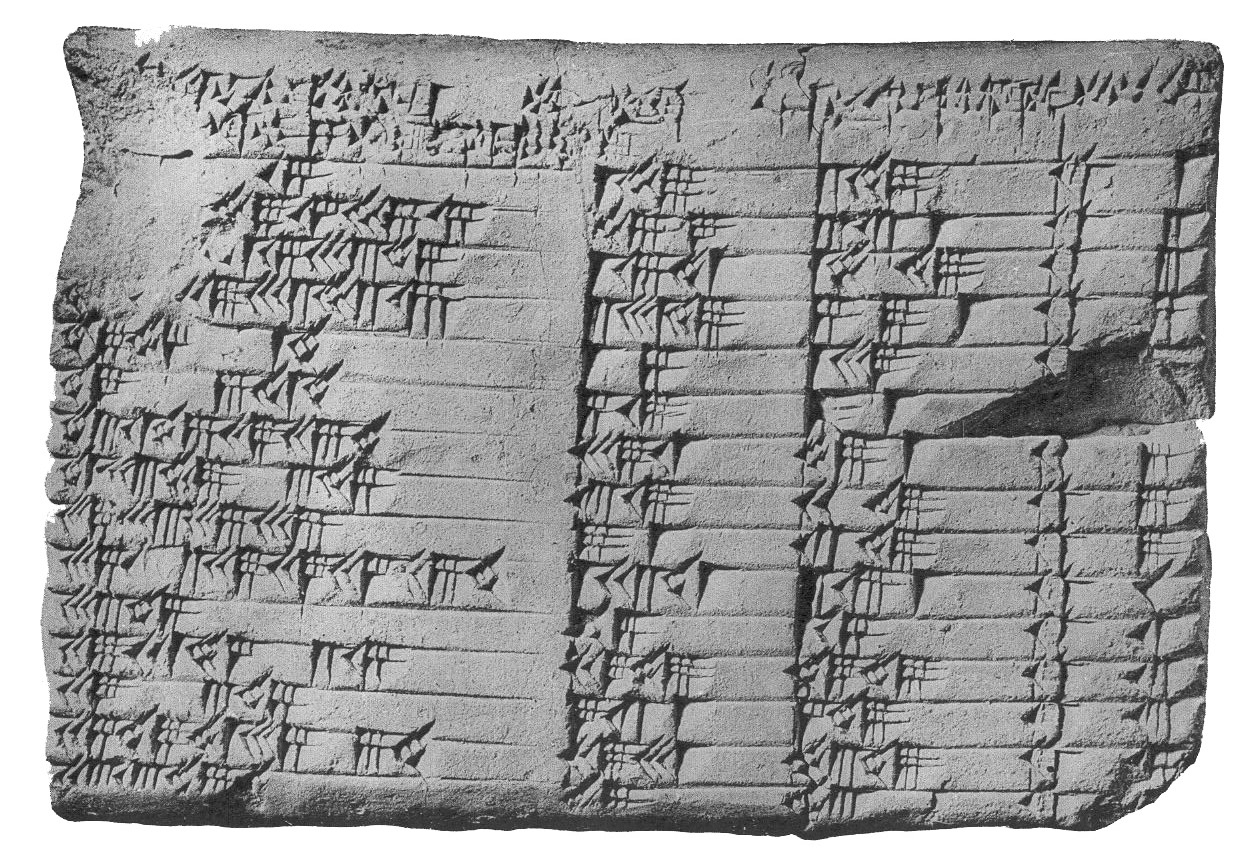
\includegraphics[width=0.68\textwidth]{Plimpton_322.jpg}
  \caption[The Babylonian tablet Plimpton 322]{The Babylonian tablet Plimpton 322, listing Pythagorean triples. }
  \label{fig:plimpton322}
\end{figure}
The triangle with side lengths $3$ and $4$ and a hypotenuse of length $5$ is sometimes called the \emph{Egyptian triangle}, since it is believed that the ancient Egyptians used this triangle for practical applications. The oldest surviving table of Pythagorean triples was created by the Babylonians, in what is now known as the tablet \emph{Plimpton 322}. This clay tablet, which is estimated to date from 1800 BCE, contains a mathematical table written in cuneiform script, where each row describes a Pythagorean triple in sexagesimal notation, i.e., base 60.

Some further Pythagorean triples include
\begin{equation*}
  (5,12,13),\qquad (21,20,29),\qquad\text{and}\qquad (15,8,17).
\end{equation*}

Fibonacci devised in his book \emph{Liber Quadratorum (The Book of Squares)} \cite{fibonacci1987} a clever way to quickly show that there are infinitely many Pythagorean triples. If an odd square $a^2$ is the $n$th odd number, i.e., if $a^2=2n+1$, then there are positive integers $b$ and $c$ such that
\begin{equation*}
  b^2 = \sum_{i=0}^{n-1}(2i+1),\qquad\text{and}\qquad c^2=\sum_{i=0}^{n}(2i+1)
\end{equation*}
by \cref{exercise:sum-of-odd-numbers}. For this choice of $a$, $b$, and $c$, we have
\begin{equation*}
  a^2 + b^2 = c^2.
\end{equation*}

\begin{proposition}
  There are infinitely many Pythagorean triples $(a,b,c)$ such that $c=b+1$.
\end{proposition}

Note that while Fibonacci used the sum of odd numbers to find a triple $(a,b,c)$ of integers such that $a^2+b^2=c^2$, these Fibonacci triples follow the pattern
\begin{equation*}
  (2b + 1) + b^2 = (b+1)^2.
\end{equation*}
Here we immediately see that if $2b+1$ is a square number $a^2$, and indeed any odd square is of this form, then we obtain a Pythagorean triple of the form $(a,b,b+1)$. Rewriting $a=2k+1$, we see that Fibonacci's Pythagorean triples are of the form
\begin{equation*}
  (2k+1,\,2k^2 + 2k,\,2k^2 + 2k+1).
\end{equation*}

The Pythagorean triples $(a,b,c)$ generated by Fibonacci's method always satisfy $c=b+1$. However, we have already seen that $(21,20,29)$ is a Pythagorean triple that is not of this form. Therefore we see that, even though Fibonacci's method can be used to see that there are infinitely many Pythagorean triples, it does not generate all of them.

In the remainder of this section we will derive the classic formula that describes all the Pythagorean triples. The method leading to this formula was described by Euclid in Book X, Proposition 29 and Book 6, Proposition 21 of the Elements.

\begin{definition}
  A \emph{primitive Pythagorean triple} is a triple $(x,y,z)$ satisfying
  \begin{equation*}
    x^2 + y^2 = z^2
  \end{equation*}
  such that $\gcd(x,y)=1$.
\end{definition}

\begin{example}
  All the Pythagorean triples generated by Fibonacci's method are primitive, since $\gcd(2b+1,b)=1$.
\end{example}

\begin{lemma}
  For any Pythagorean triple $(x,y,z)$ there is a unique primitive Pythagorean triple $(x',y',z')$ consisting of positive integers for which there is an integer $k$ such that $(kx',ky',kz')=(x,y,z)$.
\end{lemma}

\begin{proof}
  Given a Pythagorean triple $(x,y,z)$, let $k:=\gcd(x,y)$. Since $k\mid x$ and $k\mid y$, it follows from the equation $x^2+y^2=z^2$ that $k\mid z$. Thus, we define
  \begin{equation*}
    x' := x/k, \qquad y' := y/k, \qquad\text{and}\qquad z' := z/k.
  \end{equation*}
  Then $x'$ and $y'$ are relatively prime, and we have
  \begin{equation*}
    x'^2 + y'^2 = \frac{x^2+y^2}{k^2} = \frac{z^2}{k^2} = z'^2.
  \end{equation*}
  The triple $(x',y',z')$ is therefore a primitive Pythagorean triple such that
  \begin{equation*}
    (kx',ky',kz') = (x,y,z).
  \end{equation*}
  For uniqueness, suppose that $(x'',y'',z'')$ is an other such primitive Pythagorean triple, satisfying $(lx'',ly'',lz'')=(x,y,z)$. Since $\gcd(x'',y'')=1$, it follows that
  \begin{equation*}
    k=\gcd(x,y)=\gcd(lx'',ly'')=l
  \end{equation*}
  Furthermore, since at least one of $x$ or $y$ is nonzero, it follows both $k$ and $l$ are nonzero. Thus we get $x'=x''$ from the equation $kx'=kx''$, and we get $y'=y''$ from the equation $ky'=ky''$. We conclude that $(x',y',z')=(x'',y'',z'')$.
\end{proof}

By the previous lemma we can restrict our attention to primitive Pythagorean triples. Next, we do a parity analysis of the components of a primitive Pythagorean triple to show that exactly one of the components of $(x,y,z)$ in a Pythagorean triple is divisible by $4$. In \cref{exercise:divisibility-legs-pythagorean-triples} we make the similar claims that exactly one of the components of a Pythagorean triple is divisible by $3$, and exactly one divisible by $5$.

\begin{lemma}
  Consider a primitive Pythagorean triple $(x,y,z)$. Then $z$ is odd, exactly one of $x$ and $y$ is divisible by $4$, and the other is odd.
\end{lemma}

\begin{proof}
  Since $(x,y,z)$ is a primitive Pythagorean triple, it is clearly impossible for both $x$ and $y$ to be even. It is also impossible for both of them to be odd, since in that case $z^2$ would be of the form $4k+2$, which is impossible since every square is of the form $4k$ or $4k+1$. Thus, one of $x$ and $y$ is even and the other is odd. This gives us that $z^2$ is odd, which is only possible if $z$ is odd.

  It remains to show that the even component among $x$ and $y$ is in fact divisible by $4$. To this end, recall that every square is of the form $8k$, $8k+1$, or $8k+4$. Since $x^2+y^2=z^2$ is of the form $8k+1$, it is impossible for one of the squares $x^2$ or $y^2$ to be of the form $8k+4$. It follows that the even square is of the form $8k$. If $x^2$ is divisible by $8$, then clearly $x$ is divisible by $4$, and likewise if $y^2$ is divisible by $8$ then $y$ is divisible by $4$.
\end{proof}

By the previous lemma we may assume, without loss of generality, that in a primitive Pythagorean triple $(x,y,z)$, the integer $x$ is odd and the integer $y$ is even. Under this assumption, we can show that $z-x$ and $z+x$ double a square, which leads us directly to Euclid's parametrization of the Pythagorean triples.

\begin{lemma}\label{lemma:euclids-parametrization}
  Consider a primitive Pythagorean triple $(x,y,z)$ in which $y$ is even, so that $x$ is odd. Then there are two relatively prime positive integers $s<t$ of opposite parity, such that
  \begin{equation*}
    z-x=2s^2 \qquad\text{and}\qquad z+x=2t^2.
  \end{equation*}
\end{lemma}

\begin{proof}
  By the assumption that $y$ is even, we can write $y=2u$. Then we have
  \begin{equation*}
    (z-x)(z+x) = z^2-x^2 = y^2 = 4u^2.
  \end{equation*}
  Any common divisor $d$ of $z-x$ and $z+x$ must divide their sum $2z$ and their difference $2x$. However, since $x$ and $z$ are relatively prime, it follows that $d\mid 2$. On the other hand, since both $x$ and $z$ are odd it follows that $z\pm x$ is even, which implies that $d=2$. Thus we see that
  \begin{equation*}
    \left(\frac{z-x}{2}\right)\left(\frac{z+x}{2}\right)=u^2
  \end{equation*}
  is a decomposition of a square into relatively prime factors. This implies that each factor is itself a square. More precisely, there are two relatively prime positive integers $s<t$ such that
  \begin{equation*}
    \frac{z-x}{2}=s^2\qquad\text{and}\qquad\frac{z+x}{2}=t^2.
  \end{equation*}
  Furthermore, observe that since $z$ and $x$ are both odd, it follows that one of $z-x$ and $z+x$ is divisible by $4$ and the other is of the form $4k+2$. This implies that one of $s$ and $t$ is even and the other is odd.
\end{proof}

\begin{theorem}[Euclid’s Parametrization of the Pythagorean Triples]\label{theorem:euclids-parametrization}
  For every primitive Pythagorean triple $(x,y,z)$ with $y$ even, we can uniquely determine two relatively prime positive integers $s<t$ of opposite parity such that
  \begin{equation*}
    x=t^2-s^2,\qquad y=2st,\qquad\text{and}\qquad z=t^2+s^2.
  \end{equation*}
\end{theorem}

\begin{proof}
  To prove that two relatively prime integers $0<s<t$ exist as specified, we will use $s$ and $t$ as determined in \cref{lemma:euclids-parametrization}, where
  \begin{equation*}
    \frac{z-x}{2}=s^2,\qquad\text{and}\qquad\frac{z+x}{2}=t^2.
  \end{equation*}
  A simple calculation shows that $t^2-s^2=x$, and $t^2+s^2=z$. To see that $y=2st$, it suffices to show that $y^2=4s^2t^2$. This follows from the following short calculation:
  \begin{equation*}
    4s^2t^2=(z-x)(z+x)=z^2-x^2=y^2.
  \end{equation*}

  In order to show that $s$ and $t$ are uniquely determined as specified, consider additionally two relatively prime positive integers $u<v$ of opposite parity such that
    \begin{equation*}
    x=v^2-u^2,\qquad y=2uv,\qquad\text{and}\qquad z=v^2+u^2.
  \end{equation*}
  then $z-x=2u^2$ and $z+x=2v^2$, while at the same time we have $z-x=2s^2$ and $z+x=2t^2$. This implies $s^2=u^2$ and $t^2=v^2$. Since all the numbers involved are positive, we obtain that $s=u$ and $t=v$.
\end{proof}

\section{Rational Points on the Unit Circle}

The unit circle consists of all points $(u,v)$ that are a unit distance from the origin. In other words, a point $(u,v)$ in the plane with real number coordinates lies on the unit circle if it satisfies the condition
\begin{equation*}
  u^2+v^2=1.
\end{equation*}
Every Pythagorean triple $(x,y,z)$ corresponds to a point
\begin{equation*}
  \left(\frac{x}{z},\frac{y}{z}\right)
\end{equation*}
on the unit circle. Since both coordinates of the point $(\frac{x}{z},\frac{y}{z})$ are rational numbers, we say that this point is a \emph{rational point} on the unit circle.

\begin{figure}[t]
  \begin{center}
    \begin{tikzpicture}[scale=4]
      % Draw the grid with spacing 0.2, extending 0.1 beyond the square
      \draw[gray,very thin] (-1.1,-1.1) grid[step=0.2] (1.1,1.1);
      
      % Draw the thick black square
      \draw[thick,Gray] (-1,-1) rectangle (1,1);
      
      % Draw the thick black circle
      \draw[very thick] (0,0) circle (1);
      
      % Draw the x and y axes as arrows
      \draw[->] (-1.2,0) -- (1.2,0) node[right] {\(x\)};
      \draw[->] (0,-1.2) -- (0,1.2) node[above] {\(y\)};
      
      % Coordinates for the node
      \coordinate (P1) at ({117/125},{44/125});
      \coordinate (P2) at ({45/53},{-28/53});
      \coordinate (P3) at ({5/13},{12/13});
      \coordinate (P4) at ({-3/5},{4/5});
    
      
      % Draw the line from (1,1) through the node
      \draw[CornflowerBlue,very thick,dashed] (1,1) -- (P1);
      \draw[CornflowerBlue,very thick,->,shorten >=1.5ex] (P1) -- (P2);
      \draw[YellowOrange,very thick,dashed] (1,-1) -- (P2);
      \draw[YellowOrange,very thick,->,shorten >=0.8ex] (P2) -- (P3);
      \draw[Green,very thick,dashed] (1,1) -- (P3);
      \draw[Green,very thick,->,shorten >=1ex] (P3) -- (P4);
      \draw[DarkOrchid,very thick,dashed] (-1,1) -- (P4);
      \draw[DarkOrchid,very thick,->,shorten >=0.8ex] (P4) -- (1,0);
      
      % Draw the node
      \draw[fill=white,thick] (P1) circle (.5pt) node[rounded corners=2pt,right,fill=white, inner sep=1pt,xshift=1ex] {\(\left(\frac{117}{125}, \frac{44}{125}\right)\)};
      \draw[fill=white,thick] (P2) circle (.5pt) node[rounded corners=2pt,right,fill=white, inner sep=1pt,xshift=1ex,yshift=-1pt] {\(\left(\frac{45}{53},-\frac{28}{53}\right)\)};
      \draw[fill=white,thick] (P3) circle (.5pt) node[rounded corners=2pt,above,fill=white, inner sep=1pt,yshift=1.4ex] {\(\left(\frac{5}{13},\frac{12}{13}\right)\)}; 
      \draw[fill=white,thick] (P4) circle (.5pt) node[rounded corners=2pt,below,fill=white, inner sep=1pt,yshift=-1.5ex,xshift=-1ex] {\(\left(-\frac{3}{5},\frac{4}{5}\right)\)};
      \draw[fill=black,thick] (1,0) circle (.5pt);
      
    \end{tikzpicture}
  \end{center}
  \caption[Vieta jumps between rational points on the unit circle]{For any rational point $(x,y)$ on the unit circle apart from $(0,\pm1)$ and $(\pm1,0)$, draw a straight line through it from the outer corner of its quadrant to find a new rational point $(x',y')$ on the unit circle. The common denominator of $(x',y')$ is strictly smaller than that of $(x,y)$, so that this process eventually terminates at $(0,\pm1)$ or $(\pm1,0)$.}
\end{figure}

\section{The Tree of Primitive Pythagorean Triples}

The set of all primitive Pythagorean triples has the structure of a rooted ternary tree. This structure was first discovered by Berggren in 1934 \cite{berggren1934}.

\begin{equation*}
  A =
  \left(
    \begin{matrix}
      1 & -2 & 2 \\
      2 & -1 & 2 \\
      2 & -2 & 3
    \end{matrix}
  \right),\qquad
  B =
  \left(
    \begin{matrix}
      1 & 2 & 2 \\
      2 & 1 & 2 \\
      2 & 2 & 3
    \end{matrix}
  \right),\qquad\text{and}\qquad
  C =
  \left(
    \begin{matrix}
      -1 & 2 & 2 \\
      -2 & 1 & 2 \\
      -2 & 2 & 3
    \end{matrix}
  \right)
\end{equation*}

\section{Squares in Arithmetic Progressions}

\begin{wrapfigure}[16]{r}{0.4\textwidth}
  \centering
  \begin{tikzpicture}
    \node[inner sep=0pt, rounded corners=0.2em, clip] {%
      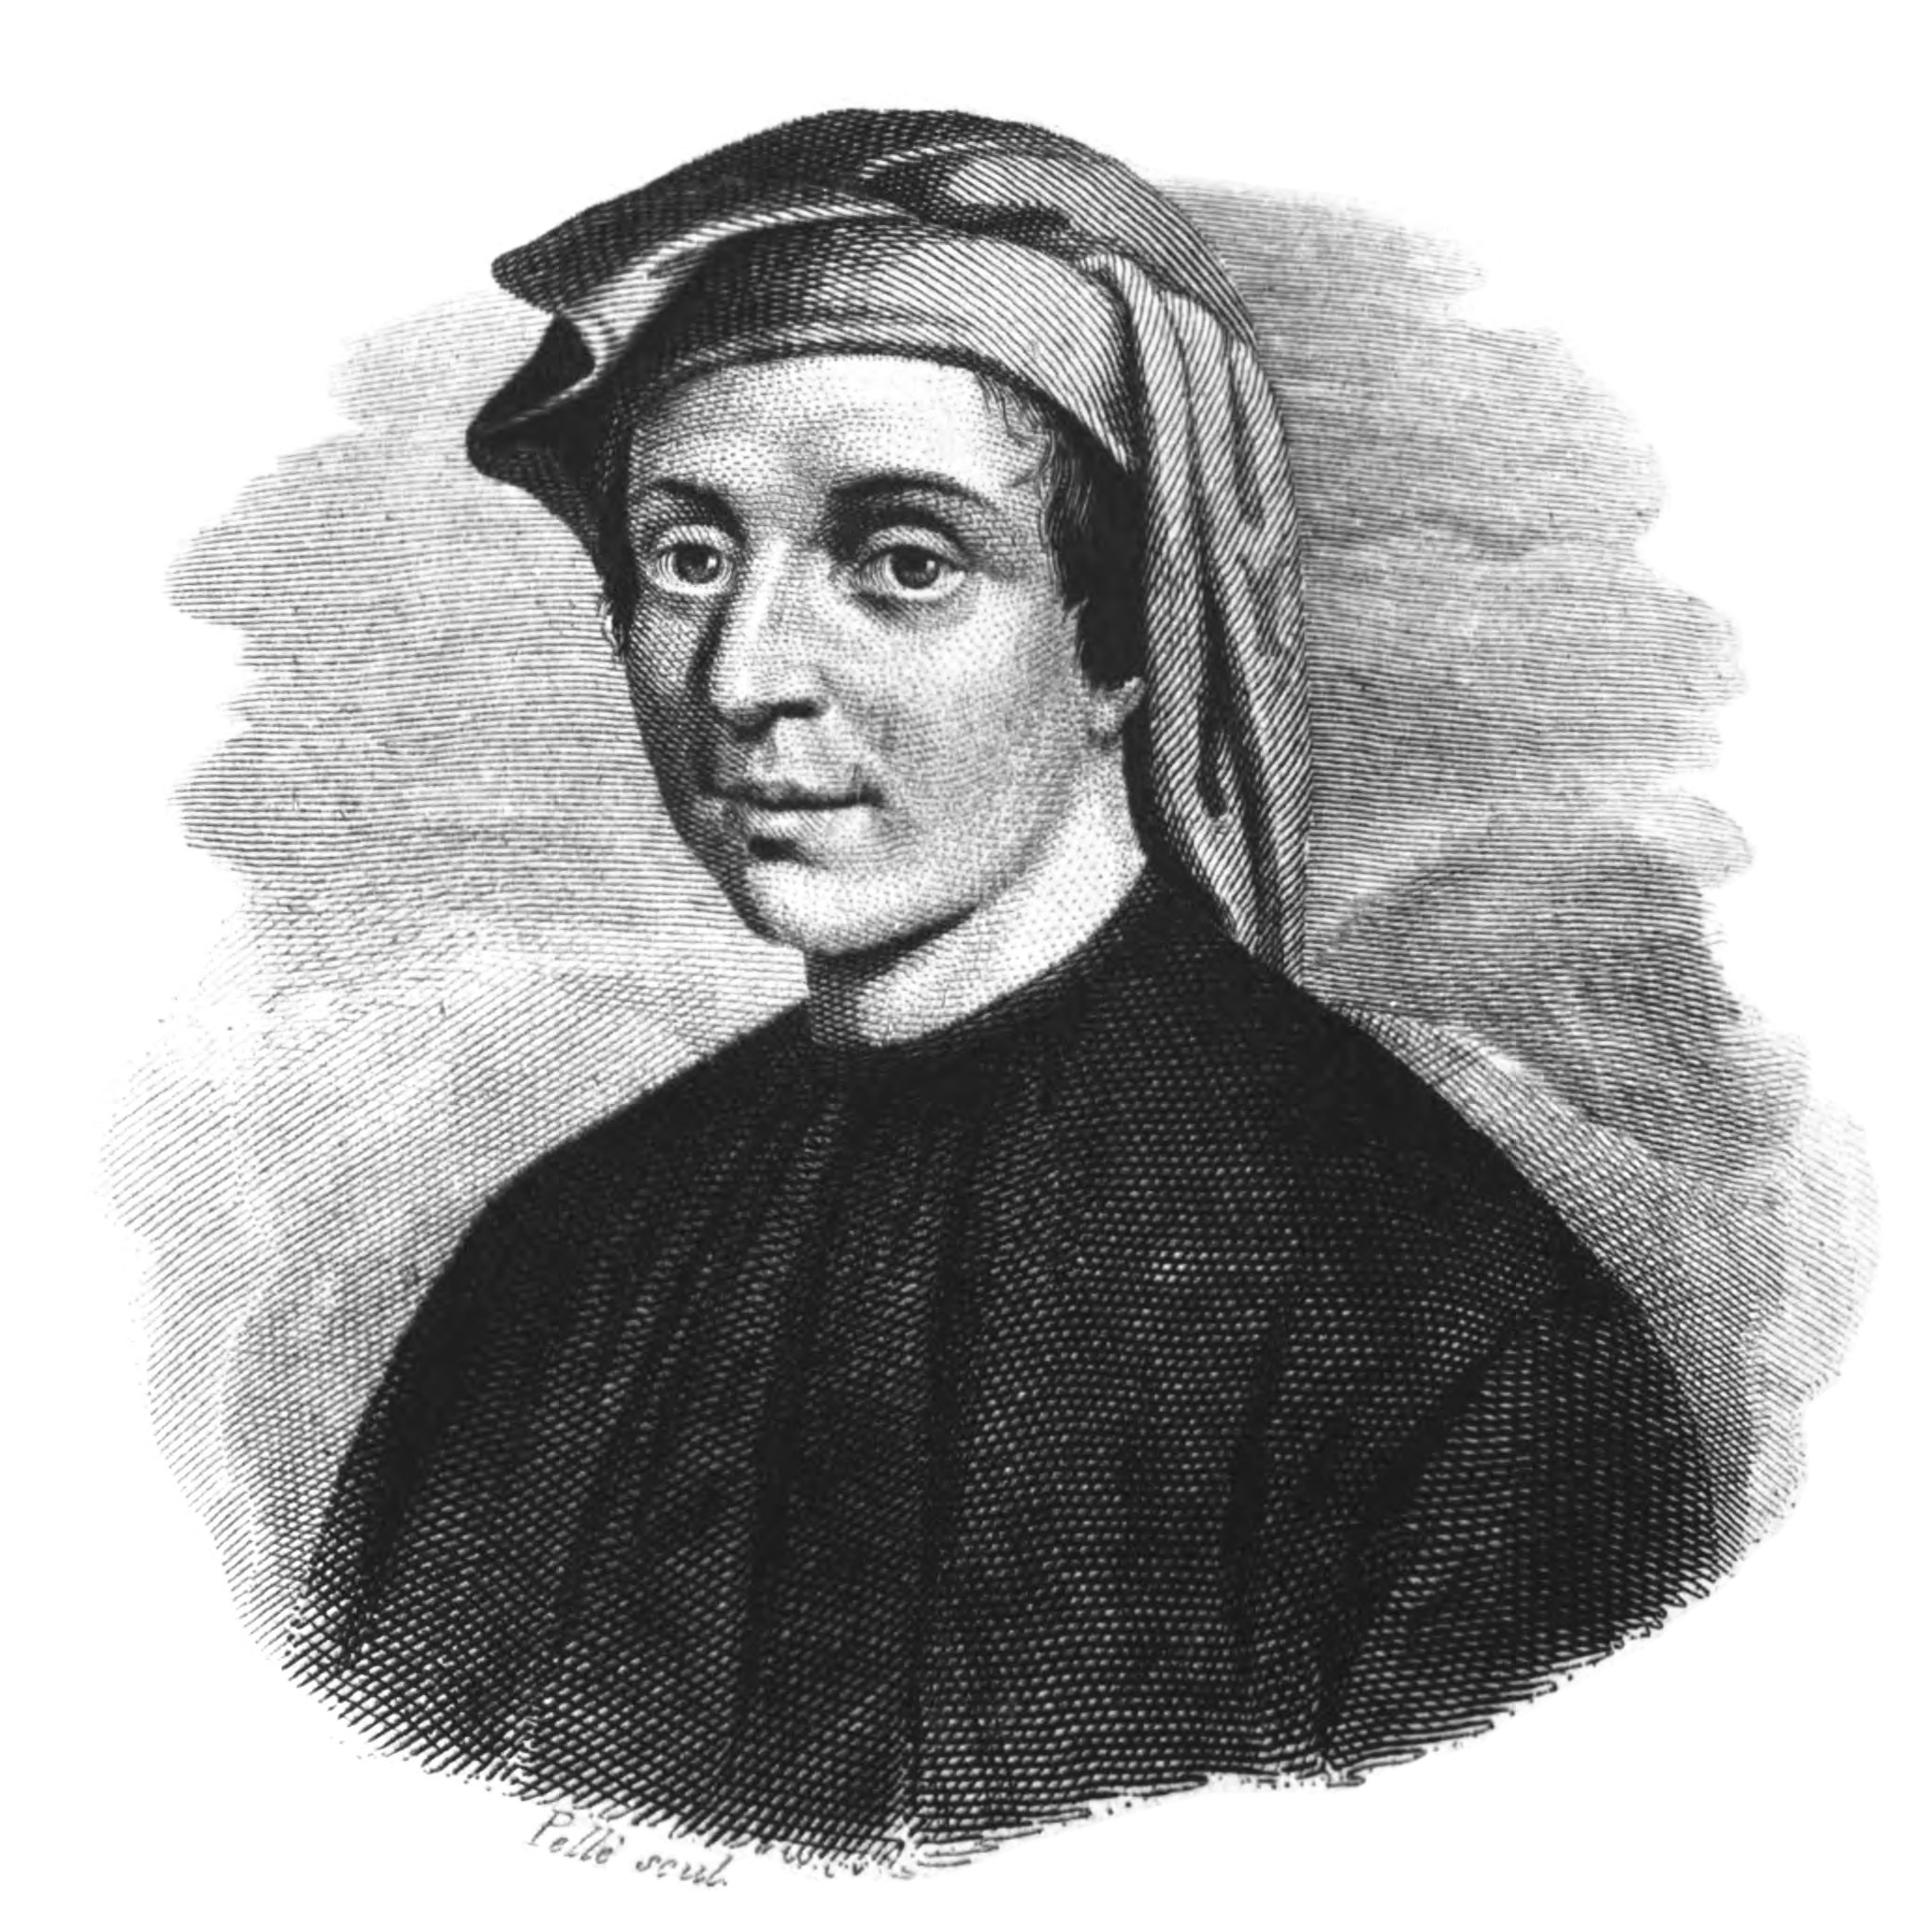
\includegraphics[width=0.38\textwidth]{Fibonacci.jpg}%
    };
  \end{tikzpicture}
  \caption[Leonardo Pisano]{\sloppy{Leonardo Pisano.}}
  \label{fig:frederick}
\end{wrapfigure}
The Euclidean parametrization of the Pythagorean triples has some further applications, but in order to get there we must make a short excursion to the city of Pisa in the 13th century, where Frederick~II reigned as the Holy Roman Emperor, and King of Sicily, Jerusalem, and Apulia. When Leonardo Pisano, more commonly known as Fibonacci, was summoned to the court of Frederick~II, he met with Master John of Palermo who challenged him with mathematical problems.

One of the challenges of Master John is stated as follows: Find a rational number $q$ such that the numbers
\begin{equation*}
  q^2-5 \qquad\text{and}\qquad q^2+5
\end{equation*}
are both squares of rational numbers. Fibonacci's investigations into this problem would eventually lead him to write his \emph{Liber Quadratorum} \cite{fibonacci1987}. The Liber Quadratorum covers topics such as Pythagorean triples, a method of generating infinitely many of them, and arithmetic progressions of squares. There were no known remaining copies of the Liber Quadratorum until a 15th century copy was rediscovered in the Biblioteca Ambrosiana in Milan, which was republished in print in 1857 by the Italian historian and mathematician Baldassarre Boncompagni Ludovisi. Today, the work available in an English translation by Laurence E.~Sigler as \emph{The Book of Squares} \cite{fibonacci1987}.

Master John's challenge is equivalently formulated as the question of finding four integers $a$, $b$, $c$, and $t$ such that
\begin{equation*}
  b^2-a^2=5t^2\qquad\text{and}\qquad c^2-b^2=5t^2.
\end{equation*}
Thus, we are looking for three squares $a^2$, $b^2$, and $c^2$ increasing in increments of $5t^2$. Thus we see that we can conveniently state the problem in terms of arithmetic triples of squares.

\begin{definition}
  An \emph{arithmetic triple of squares} is a triple $(a^2,b^2,c^2)$ consisting of integer squares such that
  \begin{equation*}
    b^2-a^2=c^2-b^2.
  \end{equation*}
  This common increment is denoted by $\Delta_{a,b,c}$, or simply $\Delta$. An arithmetic triple of squares $(a^2,b^2,c^2)$ is said to be \emph{primitive} if $\gcd(a,b,c)=1$.
\end{definition}

It follows immediately from the definition that if $(a^2,b^2,c^2)$ is a primitive arithmetic triple of squares, then $a$, $b$, and $c$ are also pairwise relatively prime.

We are thus looking for an arithmetic triple of squares, with increment of the form $\Delta:=5t^2$. In \cref{exercise:div-increment-a-p-squares} you were asked to show that the increment $\Delta$ of an arithmetic triple of squares is always divisible by $24$, which Fibonacci also reported on in Liber Quadratorum. We conclude from this observation that if $\Delta$ is of the form $5t^2$ then $\Delta$ must be a multiple of $2\cdot3\cdot 5 \cdot 24=720$.

\begin{figure}[t]
  \centering
  \resizebox{\textwidth}{!}{
    \begin{tikzpicture}
      \pgfmathdeclarefunction{dn}{1}{%
        \pgfmathparse{mod(#1,2)==1 ? #1 : int(#1/2)}%
      }

      \pgfmathtruncatemacro{\rmax}{9}
      \pgfmathtruncatemacro{\cwidth}{2*\rmax-1}
      % Loop over rows
      \foreach \row in {1,...,\rmax} {%
        
        % Vertical position
        \pgfmathsetmacro\y{(\row-1)*sqrt(3)/2}%
        
        % Columns shrink by one each row up
        \pgfmathtruncatemacro\maxc{\cwidth-(\row-1)}%
        
        \foreach \col in {1,...,\maxc} {%
          \pgfmathtruncatemacro\S{0}%
          \pgfmathtruncatemacro\J{0}%
          \pgfmathtruncatemacro\limit{\row}%
          \pgfmathloop
          \ifnum\J<\limit
            \pgfmathtruncatemacro\term{dn(\col+\J)}%
            \pgfmathtruncatemacro\S{\S+\term}%
            \pgfmathtruncatemacro\J{\J+1}%
            \repeatpgfmathloop
            \node[draw,thick,circle,minimum size=6mm,inner sep=0pt,align=center,font=\small]
              (nC\col R\row) at ({(\col-1)+(\row-1)/2},\y) {\S};%
            }%
          
        \foreach \col in {1,...,\maxc} {
          \pgfmathtruncatemacro{\ncol}{\col+1}
          \pgfmathtruncatemacro{\prow}{\row-1}
          
          \ifnum\row>1\relax
            \draw[thick] (nC\col R\row) -- (nC\col R\prow);%
            \draw[thick] (nC\col R\row) -- (nC\ncol R\prow);%
          \fi
        }%
      }%
      
      \foreach \base in {0,...,\cwidth} {%
        \pgfmathsetmacro\y{(-1)*sqrt(3)/2}
        \pgfmathtruncatemacro\pmone{\ifodd\base -1\else 1\fi}
        \pgfmathtruncatemacro\half{int((\base+1)/2)}
        \pgfmathtruncatemacro\rootval{6*\half + \pmone}
        
        \node[draw,thick,rectangle,minimum size=5.5mm,inner sep=0pt,align=center,font=\small] (b\base) at ({\base-1/2},\y) {\rootval};
        \pgfmathtruncatemacro{\leftcol}{\base}
        \pgfmathtruncatemacro{\rightcol}{\base+1}
        \ifnum\base<\cwidth
          \draw[thick] (b\base) -- (nC\rightcol R1);
        \fi
        \ifnum\base>0
          \draw[thick] (b\base) -- (nC\leftcol R1);
        \fi
      }

      % \begin{scope}[on background layer]
      %   \foreach \rowone in {1,...,\rmax}
      %   {
      %     \pgfmathtruncatemacro\maxc{\cwidth-(\rowone-1)}
      %     \foreach \colone in {1,...,\maxc}
      %     {
      %       \foreach \rowtwo in {1,...,\colone}
      %       {
      %         \pgfmathtruncatemacro\Sone{0}%
      %         \pgfmathtruncatemacro\Jone{0}%
      %         \pgfmathtruncatemacro\limitone{\rowone}%
      %         \pgfmathloop
      %         \ifnum\Jone<\limitone
      %           \pgfmathtruncatemacro\termone{dn(\colone+\Jone)}%
      %           \pgfmathtruncatemacro\Sone{\Sone+\termone}%
      %           \pgfmathtruncatemacro\Jone{\Jone+1}%
      %           \repeatpgfmathloop
                
      %         \pgfmathtruncatemacro\coltwo{\colone-\rowtwo}
      %         \pgfmathtruncatemacro\maxctwo{\cwidth-(\rowtwo-1)}
      %         \pgfmathtruncatemacro\Stwo{0}%
      %         \pgfmathtruncatemacro\Jtwo{0}%
      %         \pgfmathtruncatemacro\limittwo{\rowtwo}%
      %         \pgfmathloop
      %         \ifnum\Jtwo<\limittwo
      %           \pgfmathtruncatemacro\termtwo{dn(\coltwo+\Jtwo)}%
      %           \pgfmathtruncatemacro\Stwo{\Stwo+\termtwo}%
      %           \pgfmathtruncatemacro\Jtwo{\Jtwo+1}%
      %           \repeatpgfmathloop
                
      %         \ifnum\Sone=\Stwo\relax
      %           % fill both nodes
      %           \fill[YellowOrange] (nC\colone R\rowone) circle (3mm);
      %           \fill[CornflowerBlue] (nC\coltwo R\rowtwo) circle (3mm);
      %         \fi
      %       }
      %     }
      %   }
      % \end{scope}
      
      \begin{scope}[on background layer]
        \fill[CornflowerBlue] (nC1R1) circle (3mm);
        \fill[YellowOrange] (nC2R1) circle (3mm);
        \fill[CornflowerBlue] (nC3R2) circle (3mm);
        \fill[YellowOrange] (nC5R1) circle (3mm);
        \fill[CornflowerBlue] (nC3R3) circle (3mm);
        \fill[YellowOrange] (nC6R2) circle (3mm);
        \fill[CornflowerBlue] (nC6R3) circle (3mm);
        \fill[YellowOrange] (nC9R2) circle (3mm);
        \fill[CornflowerBlue] (nC1R9) circle (3mm);
        \fill[YellowOrange] (nC10R4) circle (3mm);
        \fill[CornflowerBlue] (nC8R5) circle (3mm);
        \fill[YellowOrange] (nC13R3) circle (3mm);
        \fill[CornflowerBlue] (nC11R3) circle (3mm);
        \fill[YellowOrange] (nC14R3) circle (3mm);
      \end{scope}
    \end{tikzpicture}
  }
  \caption[Differences of squares congruent to $1$ modulo $24$]{\label{figure:quotients-of-differences-of-squares}The numbers in squares at the base of the grid are the numbers of the form $6m\pm 1$, which correspond exactly to all the numbers $n$ such that $n^2-1$ is divisible by $24$. If $x$ and $y$ are two numbers in squares at the base of the grid, then the number $k$ at the apex of the triangle spanned by $x$ and $y$ satisfies $y^2-x^2=k\cdot 24$. For each primitive arithmetic triple $(x^2,y^2,z^2)$ of squares, the apex of the triangle spanned by $x$ and $y$ is marked in blue, and the apex of the triangle spanned by $y$ and $z$ is marked in orange.
  }
\end{figure}

The fact that the common increment in an arithmetic triple of squares is always a multiple of $24$ implies that primitive arithmetic triples of squares consist entirely of integers of the form $(6m\pm 1)^2$. Any such square exceeds a multiple of $24$ by one. This significantly reduces the search space for arithmetic triples of squares. If $a_n$ is the $n$th positive integer of the form $(6k\pm 1)^2$, then
\begin{equation*}
  d_n:=\frac{a_{n+1}-a_n}{24}=
  \begin{cases}
    n & \text{if $n$ is odd,}\\
    n/2 & \text{if $n$ is even.}
  \end{cases}
\end{equation*}
In order to determine the number of units of $24$ in the difference between two arbitrary numbers of the form $(6m\pm 1)^2$, we simply sum the numbers $d_n$: We define
\begin{equation*}
  s_{n,m}:=\sum_{i=0}^md_{n+i}=\frac{a_{n+m+1}-a_n}{24}.
\end{equation*}
Alternatively, the numbers $s_{n,m}$ are determined by the recursive rule $s_{n,m}=s_{n+1,m-1}+s_{n,m-1}-s_{n+1,m-2}$.
The numbers $s_{n,m}$ are displayed in \cref{figure:quotients-of-differences-of-squares}, from which we determine that:
    \begin{align*}
      5^2-1^2 & = 7^2-5^2 & & = 1\cdot 24, \\
      13^2 - 7^2 & = 17^2 - 13^2 & & = 5\cdot 24, \\
      17^2 - 7^2 & = 23^2 - 17^2 & & = 10\cdot 24, \\
      25^2 - 17^2 & = 31^2 - 25^2 & & = 14\cdot 24, \\ 
      29^2 - 1^2 & = 41^2 - 29^2 & & = 35\cdot 24, \\
      37^2 - 23^2 & = 47^2 - 37^2 & & = 35\cdot 24, \\
      41^2 - 31^2 & = 49^2 - 41^2 & & = 30\cdot 24.
    \end{align*}
The solution to Master John's problem to Fibonacci, which Fibonacci reported in Proposition 17 of \emph{Liber Quadratorum}, thus corresponds to the last listed arithmetic triple of squares, which gives
\begin{equation*}
  \left(\frac{41}{12}\right)^2-\left(\frac{31}{12}\right)^2=\left(\frac{49}{12}\right)^2-\left(\frac{41}{12}\right)^2=5.
\end{equation*}

% \begin{proposition}
%   If $a$, $b$, and $c$ are integers such that
%   \begin{equation*}
%     \Delta:=b^2-a^2=c^2-b^2,
%   \end{equation*}
%   then $24\mid \Delta$.
% \end{proposition}

% \begin{proof}
%   We will prove separately that $\Delta$ is of the form $8k$ and of the form $3k$. Recall that even squares are of the form $4k$, while odd squares are of the form $8k+1$, implying that differences of squares cannot be of the form $4k+2$. Since both $\Delta$ and $2\Delta$ occur as the difference of squares, where $2\Delta=c^2-a^2$, it follows that $\Delta$ must be of the form $4k$.

%   It follows that $a^2$, $b^2$, and $c^2$ are either all even or all odd. By dividing out any common factors of $a^2$, $b^2$, and $c^2$ we may assume that they are all odd, which implies that $\Delta$ is a multiple of $8$.

%   To see that $\Delta$ is a multiple of $3$, recall that all odd squares are of the form $36k+9$ or $12k+1$, so that differences of odd squares are of the form $12k$, $12k+8$, or $12k+10$. Since $\Delta=b^2-a^2$ can only be of the form $12k+8$ if $b\equiv \pm{1}\pmod{6}$ and $a\equiv 3\pmod 6$, there cannot be a square $c^2$ such that $c^2-b^2$ is also of the form $12k+8$. Likewise we rule out $12k+10$ from the possible options for $\Delta$. Thus, we conclude that $\Delta$ is a multiple of $12$, and in particular it is a multiple of $3$.
% \end{proof}

Arithmetic triples of squares are closely related to Pythagorean triples. Given an arithmetic triple of squares $(a^2,b^2,c^2)$, we can write $b^2$ as a sum of two squares written in terms of $a$ and $c$. The crucial identity that leads to the construction of a Pythagorean triple using the integers $a$, $b$, and $c$ is
\begin{equation*}
  c^2+a^2=2b^2.
\end{equation*}
Using this identity, we see that
\begin{equation*}
  \frac{(c-a)^2}{4}+\frac{(c+a)^2}{4}= \frac{c^2-2ac+a^2}{4}+\frac{c^2+2ac+a^2}{4} = \frac{c^2+ a^2}{2} = b^2.
\end{equation*}
Thus, if $(a^2,b^2,c^2)$ is an arithmetic progression of squares, then the integers
\begin{equation*}
  x := \frac{c-a}{2},\qquad y:= \frac{c+a}{2},\qquad\text{and}\qquad z:= b
\end{equation*}
determine a Pythagorean triple $(x,y,z)$. Conversely, if $(x,y,z)$ is a Pythagorean triple, then we define
\begin{equation*}
  a := |y-x|, \qquad b := z,\qquad\text{and}\qquad c:= y+x,
\end{equation*}
so that $(a^2,b^2,c^2)$ is easily seen to be an arithmetic triple of squares. Here, we defined $a$ to be the \emph{distance} between $y$ and $x$ in order to ensure that $a$ is positive. The common increment in this arithmetic triple is given by
\begin{equation*}
  z^2-(y-x)^2=2xy,
\end{equation*}
which is four times the area of the Pythagorean triangle described by the Pythagorean triple $(x,y,z)$.
The operations thus described create the following correspondence between some of the most familiar arithmetic triples of squares and Pythagorean triples:
\begin{align*}
  (1^2,5^2,7^2)   & \bimapsto (3,4,5), \\
  (7^2,13^2,17^2) & \bimapsto (5,12,13), \\
  (1^2,29^2,41^2) & \bimapsto (21,20,29), \\
  (7^2,17^2,23^2) & \bimapsto (15,8,17).
\end{align*}
The fact that these operations mapping arithmetic triples of squares to Pythagorean triples and back are mutually inverse to each other is easily verified by a few quick computations, which we leave to the reader. Thus, we have established:

\begin{theorem}\label{theorem:correspondence-arithmetic-triples-squares}
  Arithmetic triples $(a^2,b^2,c^2)$ of squares are in bijective correspondence with Pythagorean triples $(x,y,z)$, so that primitive arithmetic triples of squares correspond to primitive Pythagorean triples.
\end{theorem}

\begin{proof}
  We only prove that $(a^2,b^2,c^2)$ is a primitive arithmetic triple of squares if and only if the Pythagorean triple
  \begin{equation*}
    \left(\tfrac{c-a}{2},\tfrac{c+a}{2},b\right)
  \end{equation*}
  is primitive.

  For the forward direction, assume that $\gcd(a,b,c)=1$. To see that $(c-a)/2$ and $(c+a)/2$ are relatively prime, it suffices to show that any common divisor $d$ of $c-a$ and $c+a$ is a divisor of $2$. Indeed, if $d$ is a common divisor of $c-a$ and $c+a$, then it is also a common divisor of $2a=(c+a)-(c-a)$ and $2c=(c+a)+(c-a)$. Since $a$ and $c$ are relatively prime, it follows that $d$ is a divisor of $2$.

  Likewise, to show that $(c-a)/2$ and $b$ are relatively prime, we note that since $b$ is odd it suffices to show that $c-a$ and $b$ are relatively prime, which is only the case if $(c-a)^2$ and $b^2$ are relatively prime. This follows from
  \begin{equation*}
    (c-a)^2=c^2+a^2-2ac=2b^2-2ac,
  \end{equation*}
  since any common divisor of $(c-a)^2$ and $b^2$ is also a common divisor of $b^2$ and $2ac$, which are relatively prime by assumption. The proof that $(c+a)/2$ and $b$ are relatively prime is similar. 

  For the reverse direction, assume that
  \begin{equation*}
    \left(\tfrac{c-a}{2},\tfrac{c+a}{2},b\right)
  \end{equation*}
  is a primitive Pythagorean triple, so that $b$ is odd, and thus $b$, $(c-a)/2$, and $(c+a)/2$ are all pairwise relatively prime. Then any common divisor $d$ of $a$ and $c$ is also a common divisor of $(c-a)/2$ and $(c+a)/2$, so that $a$ and $c$ are seen to be relatively prime.

  We will prove that $(x,y,z)$ is a primitive Pythagorean triple if and only if
  \begin{equation*}
    ((y-x)^2,z^2,(y+x)^2)
  \end{equation*}
  is a primitive arithmetic triple of squares. By Euclid's parametrization of Pythagorean triples, it suffices to show that for any two
\end{proof}

The previous theorem raises an interesting point. Since the primitive Pythagorean triples are precisely described by Euclid's parametrization, there must similarly be a parametrization of the arithmetic triples of squares.

\begin{corollary}
  For any primitive arithmetic triple of squares $(a^2,b^2,c^2)$, we can uniquely determine two relatively prime positive integers $s<t$ of opposite parity such that
  \begin{equation*}
    a=2st-t^2+s^2,\qquad b=t^2+s^2,\qquad\text{and}\qquad c=2st+t^2-s^2
  \end{equation*}
  with common difference $d= 2st(t-s)^2$.
\end{corollary}

\begin{exercises}
  \exercise \emph{Bhaskara's proof of the Pythagorean Theorem.} Use the following diagram to give a proof of the \crefnamed{theorem:pythagorean-theorem}{Pythagorean Theorem}:
  \begin{equation*}
    \begin{tikzpicture}[scale=.0625,thick,line join=round,line cap=round]
      \pgfmathsetmacro{\myangle}{atan(28/45)}
      \draw (0,0) rectangle (53,53);
      \foreach \k/\x/\y in {0/0/0, 1/53/0, 2/53/53, 3/0/53}
      \draw (\x,\y) -- ++({\myangle + 90*\k}:45);
    \end{tikzpicture}
  \end{equation*}
  \exercise \label{exercise:addition-laws-sin-cos}
  \exercise \label{exercise:brahmagupta-fibonacci-identity}\emph{The Brahmagupta--Fibonacci identity.} Show that
  \begin{equation*}
    (a^2+b^2)(c^2+d^2)=(ac\pm bd)^2 + (ad\mp bc)^2.
  \end{equation*}
  Conclude that if $m$ and $n$ are two integers that can be written as the sum of two squares, then their product $mn$ can also be written as the sum of two squares.
  \exercise \label{exercise:divisibility-legs-pythagorean-triples}Consider a primitive Pythagorean triple $(x,y,z)$.
  \begin{subexenum}
  \item Prove that exactly one of $x$, $y$, and $z$ is divisible by $3$.
  \item Prove that exactly one of $x$, $y$, and $z$ is divisible by $5$.
  \item Find all Pythagorean triples $(x,y,z)$ in which $x=30$ or $y=30$. Can any of them be primitive?
    % (30,16,34),
    % (30,40,50),
    % (30,72,78),
    % (30,224,226)
  \item Find all relatively prime positive integers $x$ and $z$ such that
    \begin{equation*}
      x^2+60^2=z^2,
    \end{equation*}
    showing that the components divisible by $3$, $4$, or $5$ might all coincide.
    % (11,60,61),
    % (91,60,109),
    % (221,60,229),
    % (899,60,901).
  \end{subexenum}
  \exercise Show that for every positive integer $y$ divisible by $4$, there is a primitive Pythagorean triple of the form $(x,y,z)$.
  \exercise Show that every odd positive integer $x\geq 3$ can be written in the form $s^2-t^2$, so that there is a primitive Pythagorean triple of the form $(x,y,z)$.
  \exercise Define
  \begin{align*}
    x_n & := F_n F_{n+1}+(-1)^n, \\
    y_n & := 2F_nF_{n+1}, \\
    z_n & := F_{n}^2+F_{n+1}^2,
  \end{align*}
  where $F_k$ is the $k$th Fibonacci number. Show that $(x_n,y_n,z_n)$ is a Pythagorean triple for each $n$.
  \exercise Let
  \begin{align*}
    a_n & := F_{n}F_{n+1}- (-1)^n, \\
    b_n & := F_{n}^2 + F_{n+1}^2, \\
    c_n & := 3F_{n}F_{n+1}+(-1)^{n}.
  \end{align*}
  be defined as in \cref{exercise:arithmetic-progression-fibonacci}, so that $(a_n^2,b_n^2,c_n^2)$ is an arithmetic triple of squares. Show that
  \begin{equation*}
    \gcd(a_n,b_n,c_n)=
    \begin{cases}
      2 & \text{if $n\equiv 1\pmod{3}$,}\\
      1 & \text{otherwise.}
    \end{cases}
  \end{equation*}
    \exercise Consider three squares $a^2$, $b^2$, and $c^2$ in an arithmetic progression in increasing order.
  \begin{subexenum}
  \item Show that at least one of
    \begin{equation*}
      c-b,~c-a,~\text{and}~b-a
    \end{equation*}
    is divisible by $3$.
  \item Show that at least one of
    \begin{equation*}
      c-b,~c-a,~\text{and}~b-a
    \end{equation*}
    is divisible by $4$.
  \item Show that at least one of
    \begin{equation*}
      b~\text{and}~c-a
    \end{equation*}
    is divisible by $5$.
  \item Find all arithmetic progressions $(a^2,b^2,c^2)$ such that $c-a=60$, where only $a$ is allowed to be negative. Are there any such triples with $\gcd(a,b,c)=1$?
    % (-14,34,46),
    % (10,50,70),
    % (42,78,102),
    % (194,226,254)
  \item Find all \emph{primitive} arithmetic progressions $(a^2,b^2,c^2)$ such that $c-a=120$, where only $a$ is allowed to be negative. Hint: There are four such triples.
    % (−49,61,71)
    % (31,109,151)
    % (161,229,281)
    % (839,901,959)
  \end{subexenum}
  \exercise Find all solutions to the equation $x^2-2y^2=1$.
  \exercise \emph{Master Theodore's problem for Leonardo Pisano \cite[Proposition 24]{fibonacci1987}.} Find three positive integers $x$, $y$, and $z$ such that the numbers
  \begin{equation*}
    x+y+z+x^2,\qquad x+y+z+x^2+y^2,\qquad\text{and}\qquad x+y+z+x^2+y^2+z^2
  \end{equation*}
  are all squares.
  \exercise Find three distinct triangular numbers in an arithmetic progression.
  \exercise Find three distinct tetrahedral numbers, that is, numbers of the form $\binom{n+2}{3}$, in an arithmetic progression.
\end{exercises}

%%% Local Variables:
%%% mode: latex
%%% TeX-master: "elementary-number-theory"
%%% End:


\chapter{Infinite Descent}

\section{The Method of Infinite Descent}

The method of infinite descent was invented by Fermat. He used this method effectively to solve various problems, including that there are no solutions to $x^4+y^4=z^4$ in the positive integers, and that the area of a right triangle is not a perfect square. The method of infinite descent is used to show that certain properties or identities are impossible, by showing that if they do hold then an infinitely descending sequence of natural numbers can be constructed. The following theorem shows that there is no such sequence.

\begin{proposition}\label{proposition:infinite-descent}
  There is no infinite descending sequence
  \begin{equation*}
    a_0 > a_1 > a_2 > \cdots
  \end{equation*}
  of natural numbers.
\end{proposition}

\begin{proof}
  Suppose, by way of contradiction, that there is such a sequence
  \begin{equation*}
    a_0 > a_1 > a_2 > \cdots.
  \end{equation*}
  Then the set
  \begin{equation*}
    A:=\{a_0,a_1,a_2,\ldots\}
  \end{equation*}
  is a nonempty subset of the natural numbers, and by the \crefnamed{theorem:well-ordering-natural-numbers}{well-ordering principle} of the natural numbers it follows that this set has a least element. However, all the elements in $A$ are of the form $a_n$ for some natural number $\mathbb{N}$, and none of these elements are minimal, since we have assumed that $a_n>a_{n+1}$. This contradiction shows that our assumption that there exists an infinite descending sequence must be false, and thus there is no such sequence.
\end{proof}

The previous proposition leads to Fermat's method of infinite descent. Fermat observed that if an assumption $H$ leads to an infinite descending sequence, then the assumption $H$ must be false. %We will illustrate Fermat's method with the following theorem:

%In the previous proof we introduced a set $A$ of which the elements were pairs $(a,b)$ of natural numbers satisfying $a^2=nb^2$, and we defined a function $f:A\to A$ in order to show that $A$ is empty. In the following theorem we state the method of infinite descent using a generalization of this setup.

\begin{theorem}[Method of Infinite Descent]\label{theorem:method-of-descent}
  Consider a set $A$ equipped with a function $f:A\to A$ and a function $h:A\to\mathbb{N}$. If $h(f(a))<h(a)$ for all $a$, then $A$ is empty.
\end{theorem}

\begin{proof}
  Suppose, by way of contradiction, that the set $A$ is inhabited by an element $a\in A$. By iterating $f$, we define a sequence of elements $a_i$ by
  \begin{align*}
    a_0 & := a \\
    a_{i+1} & := f(a_i).
  \end{align*}
  Then we have $h(a_0)>h(a_i)>h(a_2)>\cdots$, which is an infinite descending sequence of natural numbers. Thus, the assumption that $A$ is inhabited was false.
\end{proof}

\section{The Area of a Pythagorean Triangle is not a Square}

A classic application of Fermat's infinite descent gives us that the area of a Pythagorean triangle is never a square number. Recall that the area of a triangle is half the base times the height, so that every Pythagorean triple $(a,b,c)$ determines a Pythagorean triangle with area
\begin{equation*}
  \frac{1}{2}ab.
\end{equation*}

\begin{theorem}\label{theorem:is-not-square-area-pythagorean-triangle}
  The area of a Pythagorean triangle is not a square number.
\end{theorem}

\begin{proof}
  It suffices to prove the statement for primitive Pythagorean triangles; that is, a triangle whose sides $(a,b,c)$ form a primitive Pythagorean triple. By \crefnamed{theorem:euclids-parametrization}{Euclid's parametrization of the Pythagorean triples}, we can find two relatively prime integers $s<t$ of opposite parity, such that
  \begin{equation*}
    a=t^2-s^2,\qquad b=2st,\qquad\text{and}\qquad c=t^2+s^2.
  \end{equation*}
  The area of the triangle is given in terms of this parametrization by the nonzero quantity
  \begin{equation*}
    st(t^2-s^2)=st(t-s)(t+s).
  \end{equation*}
  Now observe that all of these factors are relatively prime to one another; indeed, given that $s$ and $t$ are relatively prime, this follows at once from \cref{proposition:gcd-euclidean-division}. Thus we conclude that if the area of the Pythagorean triangle is a square, then each of these factors must also be a square. This allows us to write
  \begin{equation*}
    s=u^2,\quad t=v^2,\quad t-s=x^2,\quad\text{and}\quad t+s=y^2.
  \end{equation*}
  Since $s$ and $t$ are of opposite parity, it follows that $x$ and $y$ are both odd. Now notice that the triple of integers
  \begin{equation*}
    \left(\frac{y-x}{2},\frac{y+x}{2},v\right)
  \end{equation*}
  is a Pythagorean triple, since
  \begin{equation*}
    \left(\frac{y-x}{2}\right)^2+\left(\frac{y+x}{2}\right)^2=\frac{y^2+x^2}{2}=v^2.
  \end{equation*}
  Furthermore, the area of the corresponding Pythagorean triangle is given by
  \begin{equation*}
    \frac{1}{2}\left(\frac{y-x}{2}\right)\left(\frac{y+x}{2}\right)=\frac{y^2-x^2}{8}=\frac{u^2}{4}.
  \end{equation*}
  The quantity $u^2/4$ must therefore be an integer strictly less than $s$, which in turn is strictly less than the area $\frac{1}{2}ab$. Thus, we have constructed a Pythagorean triangle whose area is a strictly smaller nonzero square number, which leads to a contradiction by infinite descent.
\end{proof}

\section{The Unsolvability of \texorpdfstring{$x^4+y^4=z^4$}{x⁴ + y⁴ = z⁴}}

\begin{theorem}
  There are no three positive integers $x$, $y$, and $z$ for which the equation
  \begin{equation*}
    x^4+y^4=z^2
  \end{equation*}
  holds.
\end{theorem}

\begin{proof}
  Consider the set
  \begin{equation*}
    A:=\{(x,y,z)\in\mathbb{Z}_{>0} \mid x^4+y^4=z^2\}
  \end{equation*}
  with $h(x,y,z):=z$. We will construct a function $f:A\to A$ such that $h(f(x,y,z))<h(x,y,z)$ for every $(x,y,z)\in A$.
  
  First, we notice that if $(x,y,z)$ is a triple of positive integers satisfying the equation $x^4+y^4=z^2$, then $(x^2,y^2,z)$ is a Pythagorean triple. Since we can always divide out any common factors, we may assume that $x$ and $y$ are relatively prime. Furthermore, we may assume that $y$ is even, so that by Euclid's parametrization there are relatively prime positive integers $s<t$ of opposite parity such that
  \begin{align*}
    x^2 & = t^2-s^2, \\
    y^2 & = 2st, \\
      z & = t^2+s^2.
  \end{align*}

  The key observation is now in the first equation: We obtain a new Pythagorean triple $x^2+s^2=t^2$, allowing us to apply Euclid's parametrization of Pythagorean triples once more. Since $x$ is odd it follows that $s$ is even, so we find relatively prime positive integers $u<v$ such that
  \begin{align*}
    x & = v^2-u^2 \\
    s & = 2uv \\
    t & = v^2+u^2.
  \end{align*}
  Now it follows that $y^2 = 4uv (v^2+u^2)$. We claim that the numbers $uv$ and $v^2+u^2$ are relatively prime. To see this, note that both $u$ and $v$ are relatively prime to $v^2+u^2$ since
  \begin{equation*}
    \gcd(u,v^2+u^2)=\gcd(u,v^2)=1\qquad\text{and}\qquad\gcd(v,v^2+u^2)=\gcd(v,u^2)=1,
  \end{equation*}
  and hence their product $uv$ is also relatively prime to $v^2+u^2$.

  Since $uv$ and $v^2+u^2$ are relatively prime, the fact that $4uv(v^2+u^2)$ is a square implies that both $uv$ and $v^2+u^2$ are squares. Given that $u$ and $v$ are relatively prime, this implies that $u$ and $v$ are squares, i.e., that there are integers $a$ and $b$ such that $u=a^2$ and $v=b^2$. Thus, it follows that
  \begin{equation*}
    v^2+u^2=a^4+b^4
  \end{equation*}
  is a square, say $c^2$. We have therefore shown that any triple of positive integers $x$, $y$, and $z$ such that $x^4+y^4=z^2$ we can construct positive integers $a$, $b$, and $c$ such that
  \begin{equation*}
    a^4 + b^4 = c^2.
  \end{equation*}
  This finishes the construction of the function $f:A\to A$. Furthermore, the strict inequality $c^2=s<s^2+t^2=z^2$ shows that $h(f(x,y,z))<h(x,y,z)$, so we conclude by the \crefnamed{theorem:method-of-descent}{method of infinite descent} that the set $A$ must be empty.
\end{proof}

\begin{corollary}
  There is no solution to the equation
  \begin{equation*}
    x^{4}+y^{4}=z^{4},
  \end{equation*}
  where $x$, $y$, and $z$ are positive integers.
\end{corollary}

\begin{proof}
  Given such a solution, set $a=x$, $b=y$, and $c=z^{2}$. Then we have
  \begin{equation*}
    a^4+b^4=c^2,
  \end{equation*}
  which is impossible.
\end{proof}

\section{The Nonexistence of Four Squares in an Arithmetic Progression}

We have shown in \cref{theorem:correspondence-arithmetic-triples-squares} that there is a bijective correspondence between arithmetic triples of squares and Pythagorean triples. It is natural to wonder whether there are any longer arithmetic progressions of squares. Fermat posed this problem in his correspondence with Bernard Frénicle de Bessy in 1640, and noted that it was impossible to find four such squares. The first publicly known proof is due to Euler. Here we will follow a proof of Alf van der Poorten \cite{vanderpoorten2007}, who observed that any four pairwise relatively prime squares $a^2$, $b^2$, $c^2$, and $d^2$ in an arithmetic progression determine, besides the Pythagorean triples corresponding to $(a^2,b^2,c^2)$ and $(b^2,c^2,d^2)$, a third Pythagorean triple. To see this, assume the step size is a number of the form $2n$, where it follows from \cref{exercise:div-increment-a-p-squares} that $n$ is divisible by $12$, and let $x$ be the average of $b^2$ and $c^2$ so that $b^2=x-n$ and $c^2=x+n$. Then the number $y:=abcd$ satisfies
\begin{equation*}
  y^2=a^2b^2c^2d^2=(x-3n)(x-n)(x+n)(x+3n)=(x^2-n^2)(x^2-9n^2).
\end{equation*}
By completing the square, we see that
\begin{equation*}
  y^2=x^4-10n^2x^2+9n^4=(x^2-5n^2)^2-16n^4.
\end{equation*}
Thus we obtain a Pythagorean triple
\begin{equation*}
  y^2+(4n^2)^2=(x^2-5n^2)^2.
\end{equation*}
Since $a$, $b$, $c$, and $d$ are assumed to be relatively prime, the number $y$ is relatively prime to $4n$ and thus to $x$ and $x^2-5n^2$. This implies that our newly obtained Pythagorean triple is primitive. This Pythagorean triple is our entry into a descent argument.

\begin{lemma}
  For every four pairwise relatively prime squares $a^2$, $b^2$, $c^2$, and $d^2$ in an arithmetic progression we can uniquely determine a pair of relatively prime positive integers $u$ and $v$ such that $4u^2+v^2$ and $u^2+v^2$ are both squares, and the step size in the arithmetic progression of squares is $2uv$.
\end{lemma}

\begin{proof}
  Consider four pairwise relatively prime squares $a^2$, $b^2$, $c^2$, and $d^2$ in an arithmetic progression, where $a$, $b$, $c$, and $d$ are assumed to be relatively prime numbers of the form $6k\pm 1$, and the step size is a number of the form $2n$ so that $n$ is divisible by $12$. As previously shown, we obtain a primitive Pythagorean triple
  \begin{equation*}
    y^2+(4n^2)^2=(x^2-5n^2)^2,
  \end{equation*}
  where $y=abcd$ and $x$ is the average of $b^2$ and $c^2$.
  

  By averaging $b^2$ and $c^2$, we obtain a number $x$ such that
  \begin{equation*}
    a^2=x-3n,\qquad b^2=x-n,\qquad c^2=x+n,\qquad\text{and}\qquad d^2=x+3n.
  \end{equation*}
  Thus, the product of these four squares is of the form
  \begin{equation*}
    y^2=a^2b^2c^2d^2= (x^2-n^2)(x^2-9n^2).
  \end{equation*}
  By completing the square, we see that
  \begin{equation*}
    y^2=x^4-10n^2x^2+9n^4=(x^2-5n^2)^2-16n^4.
  \end{equation*}
  Thus we obtain a Pythagorean triple
  \begin{equation*}
    y^2+(4n^2)^2=(x^2-5n^2)^2.
  \end{equation*}
  Since $a$, $b$, $c$, and $d$ are assumed to be relatively prime, the number $y$ is relatively prime to $4n$ and thus to $x$ and $x^2-5n^2$. This implies that our newly obtained Pythagorean triple is primitive. Thus there are relatively prime positive integers $2s$ and $t$ such that
  \begin{equation*}
    y=|t^2-4s^2|,\qquad 4n^2=4st,\qquad\text{and}\qquad x^2-5n^2=t^2+4s^2.
  \end{equation*}
  Since $n^2=st$ and $s$ and $t$ are relatively prime, it follows that $s=u^2$, $t=v^2$, and $uv=n$. We obtain that
  \begin{equation*}
    y=|v^4-4u^4|,\qquad 4n^2=4u^2v^2,\qquad\text{and}\qquad x^2=v^4+5u^2v^2+4u^4=(v^2+4u^2)(v^2+u^2).
  \end{equation*}
\end{proof}

\begin{theorem}[Fermat--Euler]
  Every arithmetic progression of length four of the integer squares is constant.
\end{theorem}

\begin{proof}
  Consider four squares $a^2$, $b^2$, $c^2$, and $d^2$ in an arithmetic progression. Then there exist relatively prime positive integers $s<t$ of opposite parity and relatively prime positive integers $u,v$ of opposite parity such that
  \begin{align*}
    t^2+s^2 = b & = |2uv - v^2 + u^2|, \\
    2st + t^2 - s^2 = c & = v^2+u^2.
  \end{align*}
  There are two cases to consider. If we assume that $2uv - v^2 + u^2$ is nonnegative, then adding and subtracting both sides from each other and dividing by $2$ give the identities
  \begin{align*}
    s(t-s) & = v(v-u), \\
    t(t+s) & = u(v+u).    
  \end{align*}
  Those equations added together yield $b=s^2+t^2=u^2+v^2=c$, so that the arithmetic progression $(a^2,b^2,c^2,d^2)$ is shown to be constant.
  
  If, on the other hand, we assume that $2uv - v^2 +u^2$ is negative, then we obtain that
  \begin{equation*}
    2(t^2+s^2)^2 - (2st+t^2-s^2)^2
  \end{equation*}
  similarly the identities
  \begin{align*}
    s(t-s) & = u(v+u), \\
    t(t+s) & = v(v-u).
  \end{align*}
  We claim that there are no solutions with $0<s<t$ and $0<u<v$ of this system of equations. The second equation is a quadratic equation in $t$, with discriminant $s^2+4v(v-u)$. Thus, if there is to be a solution to the given system of equations, each equation seen as a quadratic equation in one variable $s$, $t$, $u$, or $v$ must have a square discriminant:
  \begin{align*}
    t^2+4u(v+u) & = k^2, \\
    u^2+4t(t+s) & = l^2, \\
    s^2+4v(v-u) & = m^2, \\
    v^2+4s(t-s) & = n^2, \\
  \end{align*}
  Notice that the first two equations are the same up to swapping the roles of $t$ and $u$ and the roles of $s$ and $v$. Likewise, the last two equations are the same up to a similar swap of variables.
  \begin{equation*}
    k^2-l^2 = t^2-u^2 + 4(u(v+u) - t(t+s)) = (t-u)(t+u)+ 4(t-u)(t+u+s) = t^2+ts-u^2-us
  \end{equation*}
\end{proof}

\section{The Congruent Number Problem}

Recall from \cref{sec:squares-in-aps} the challenge that Master John posed in the early 13th century to Leonardo Fibonacci: To find a rational number $q$ such that both
\begin{equation*}
  q^2-5,\qquad\text{and}\qquad q^2+5
\end{equation*}
are both rational. Or equivalently, to find a Pythagorean triangle whose area is five times a square. Master John must somehow have known that the number $5$ in his challenge was special: It is the smallest positive integer for which his challenge has a solution.

\begin{definition}
  A positive integer $a$ is said to be a \emph{congruent number} if it occurs as the area of a right triangle with rational sides and rational hypotenuse.
\end{definition}

The following lemma rephrases the condition of being a congruent number in terms of Pythagorean triangles.

\begin{lemma}\label{lemma:congruent-numbers}
  A number $n$ is congruent if and only if there is a primitive Pythagorean triangle whose area is $n$ times a square.
\end{lemma}

\begin{proof}
  Consider three rational numbers $a$, $b$, and $c$ such that
  \begin{equation*}
    a^2+b^2=c^2,\qquad\text{and}\qquad \frac{ab}{2}=n,
  \end{equation*}
  so that $n$ is presented as the area of a right triangle with rational sides and hypotenuse. By multiplying $a$, $b$, and $c$ with $m$, which we define to be the least common multiple of the denominators of $a$ and $b$, we obtain integers $A:= ma$, $B:= mb$, and $C:= mc$ such that
  \begin{equation*}
    A^2+B^2=C^2,\qquad\text{and}\qquad \frac{AB}{2}=nm^2
  \end{equation*}
  so that $(A,B,C)$ constitutes a Pythagorean triple whose area is $n$ times a square. By dividing out any common divisors, we obtain a primitive such Pythagorean triangle. Since this process is clearly reversible, this proves the claim.
\end{proof}

\begin{theorem}
  No square positive integer is a congruent number.
\end{theorem}

\begin{proof}
  This claim follows from \cref{lemma:congruent-numbers} and Fermat's \cref{theorem:is-not-square-area-pythagorean-triangle}, which states that the area of a Pythagorean triangle cannot be a square.
\end{proof}

We will show in the following theorem that the number $2$ is not congruent. The noncongruence of the number $3$ is stated as an exercise. Having the integers $1$, $2$, $3$, and $4$ ruled out as congruent numbers, we see indeed that $5$ is the least congruent number.

\begin{theorem}
  If a positive integer is twice a square, then it isn't congruent.
\end{theorem}

\begin{proof}
  This theorem can be stated equivalently as: The area of a primitive Pythagorean triangle cannot be twice a square. To derive a contradiction, we assume that a Pythagorean triple $(A,B,C)$ exists with
  \begin{equation*}
    \frac{AB}{2}=2m^2.
  \end{equation*}
  By Euclid's parametrization of the primitive Pythagorean triples, a Pythagorean triple as described above is uniquely determined by a pair of relatively prime positive integers $s<t$ of opposite parity, with
  \begin{equation*}
    A=t^2-s^2,\qquad B=2st,\qquad\text{and}\qquad C:=t^2+s^2.
  \end{equation*}
  Using this parametrization, we find the following equation for the area:
  \begin{equation*}
    st(t^2-s^2)=2m^2.
  \end{equation*}
  However, the integers $s$, $t$, and $t^2-s^2$ are all relatively prime, which implies that exactly one of them---either $s$ or $t$---is twice a square and the other two are squares.
\end{proof}

Determining which numbers are congruent turns out to be an incredibly difficult problem, which is still unsolved. This problem is called the \emph{congruent number problem}, and via Tunnell's theorem it has connections to the famous Birch and Swinnerton--Dyer conjecture.

\section{Vieta Jumping}

Consider a polynomial with roots $a_1$, $a_2$, and $a_3$, i.e., the polynomial
\begin{equation*}
  (x-a_1)(x-a_2)(x-a_3).
\end{equation*}
If we expand this polynomial, it takes the form
\begin{equation*}
  x^3-(a_1+a_2+a_3)x^2+(a_1a_2+a_2a_3+a_3a_1)x-a_1a_2a_3.
\end{equation*}
François Vi\`ete recognized in the 16th century that this yields a relation between the coefficients and the roots of a monic polynomial, i.e., a polynomial with leading coefficient $1$. In the case of a monic polynomial $x^3+c_2x^2+c_1x+c_0$ with roots $a_1$, $a_2$, and $a_3$, we get
\begin{align*}
  c_2 & = -(a_1+a_2+a_3) \\
  c_1 & = a_1a_2+a_1a_3+a_2a_3 \\
  c_0 & = -a_1a_2a_3.
\end{align*}

More generally, the coefficients of the polynomial
\begin{equation*}
  f(x)=(x-a_1)\cdots (x-a_n)
\end{equation*}
are of the form
\begin{equation*}
  e_k(a_1,\ldots,a_n):=\sum_{1\leq i_1<i_2<\cdots<i_k\leq n}a_{i_1}a_{i_2}\cdots a_{i_k}.
\end{equation*}
Notice that these coefficients are themselves polynomials in the variables $a_1,\ldots,a_n$. These polynomials are called the \emph{elementary symmetric polynomials}. For example, for $n=3$ we have
\begin{equation*}
  f(x)=x^3-(a_1+a_2+a_3)x^2+(a_1a_2+a_1a_3+a_2a_3)x-a_1a_2a_3.
\end{equation*}

Vieta jumping is a modern problem-solving technique that became popular in international contest problems.

\begin{example}
  In \cref{exercise:div-product-sum-of-squares} you were asked to show that for any two positive integers $x$ and $y$ such that $xy\mid x^2+y^2$, we must have $x=y$. The expected solution was to observe that the discriminant of the quadratic equation $x^2-kxy+y^2=0$ seen as an equation in one variable $x$ and a parameter $y$ is $(ky)^2-4y^2$, which is a square if and only if $k=2$. Although this problem can readily be solved directly, we will use it here to illustrate Vieta jumping.

  We first observe that the quadratic equation
  \begin{equation*}
    x^2-kxy + y^2=0
  \end{equation*}
  arising from the divisibility condition $xy\mid x^2+y^2$ is \emph{homogeneous} in the sense that each of the three terms have the same degree in $x$ and $y$ combined. Thus, if $x$ an $y$ satisfy this polynomial equation, then so must
  \begin{equation*}
    x' :=\frac{x}{\gcd(x,y)}\qquad\text{and}\qquad y':=\frac{y}{\gcd(x,y)}.
  \end{equation*}
  We can therefore solve the problem by showing that the only pair of coprime positive integers $x$ and $y$ satisfying the polynomial equation must satisfy $x=y=1$.

  To see this, we may assume without loss of generality that $0<y<x$. Given that $x$ is a solution of the quadratic equation $t^2-kty+y^2$ in the variable $t$, it follows that the other solution is $x':=ky-x$. Notice that $\gcd(ky-x,y)=1$, so that $x':=ky-x$ and $y$ are again relatively prime. Furthermore, since $xx'=y^2$ it follows that
  \begin{equation*}
    0<x'=\frac{y^2}{x}<y.
  \end{equation*}
  We have thus found a new solution with $x'<y$. Now we can swap the roles for $x'$ and $y$ and repeat the process, obtaining every smaller solutions in the positive integers. Since this is clearly impossible, it must have been impossible for there to be a pair of relatively prime positive integers $x$ and $y$ such that $xy\mid x^2+y^2$.
\end{example}

\begin{exercises}
  \exercise Use the method of infinite descent to show that if $a$ and $b$ are relatively prime and the product $ab$ is a square, then both $a$ and $b$ are squares.
  \exercise Show that there are no positive integer squares of the form
  \begin{equation*}
    x^2+xy+y^2.
  \end{equation*}
  \exercise Show that there are no positive integer squares of the form
  \begin{equation*}
    2x^2+2xy+2y^2.
  \end{equation*}
  \exercise Show that there are no integer solutions to the equation
  \begin{equation*}
    x^2+y^2=3t^2
  \end{equation*}
  such that $t>0$.
  \exercise Show that there are no integer solutions to the equation
  \begin{equation*}
    x^2+y^2+z^2=7t^2
  \end{equation*}
  such that $t>0$.
  \exercise Let $x$ and $y$ be positive integers satisfying the equation
  \begin{equation*}
    x^2-xy+y^2=1.
  \end{equation*}
  Prove that $x=y=1$.
  \exercise Show that if $x$ and $y$ are positive integers such that $xy$ divides $x^2+y^2+1$, then
  \begin{equation*}
    \frac{x^2+y^2+1}{xy}=3.
  \end{equation*}
  \exercise Let $x$, $y$, and $z$ be positive integers such that $xy+yz+zx$ divides $x^2+y^2+z^2$. Prove that
  \begin{equation*}
    \frac{x^2+y^2+z^2}{xy+yz+zx}
  \end{equation*}
  is a perfect square.
  \exercise Prove that the area of a Pythagorean triangle cannot be twice a square.
  \exercise Prove that the Diophantine equation
  \begin{equation*}
    x^4-y^4=z^2
  \end{equation*}
  has no solutions in the positive integers.
  \exercise Show that the only triangular number which is also a fourth power is $1$.
\end{exercises}

%%% Local Variables:
%%% mode: latex
%%% TeX-master: "elementary-number-theory"
%%% End:


\part{The Multiplicative Nature of Numbers}

\chapter{Prime Numbers}\label{chapter:fundamental-theorem-of-arithmetic}

\section{The Fundamental Theorem of Arithmetic}

\begin{definition}
  An integer $a$ is said to be \emph{prime} if it has exactly one positive proper divisor. Any integer $a\neq \pm 1$ that is not prime is said to be a \emph{composite number}.
\end{definition}

The numbers $0$ and $1$ are not prime. To see that $0$ isn't prime, simply note that any positive integer is a proper divisor of $0$. To see that $1$ isn't prime, note that $1$ doesn't have any proper divisors. Indeed, it has exactly one positive divisor, namely $1$ itself, but this divisor isn't proper. We also note that if $a>1$ is prime, then the number $1$ is always a positive proper divisor. Thus we see that $a>1$ is prime if and only if the number $1$ is its unique positive proper divisor.

To see that the number $2$ is prime, note that its positive divisors are a subset of the set $\{1,2\}$ consisting of all the positive integers below $2$. Its proper divisors are therefore a subset of $\{1\}$. The integer $1$ is indeed a positive divisor, so we see that $2$ has exactly one positive proper divisor.

To see that the number $3$ is prime, note that its positive divisors are a subset of the set $\{1,2,3\}$ consisting of all positive integers below $3$. The number $1$ is a proper divisor, the number $2$ doesn't divide $3$, and $3$ itself is a divisor but it isn't proper. Therefore we see that the number $3$ has exactly one positive proper divisor.

The number $4$ isn't prime, because the numbers $1$ and $2$ are two distinct proper divisors of $4$. This process of finding all primes up to a desired bound is formalized in the \emph{sieve of Eratosthenes}, which we will now describe. \cref{figure:sieve-of-eratosthenes} displays the sieve of Eratosthenes up to 1350.

\begin{figure}[!p]
\centering
\resizebox{\textwidth}{!}{%
\begin{tikzpicture}[x=0.5cm,y=0.5cm]

  % PARAMETERS
  \def\Cols{30}                       % number of columns
  \def\N{1350}                        % max number
  \pgfmathsetmacro{\Rows}{ceil(\N/\Cols)}  % computed number of rows
  \def\CirDiam{0.4cm}                 % diameter of every circle

  % 1) draw every number in a white circle of fixed size
  \foreach \i in {1,...,\N} {
    \pgfmathtruncatemacro{\c}{mod(\i-1,\Cols)}
    \pgfmathtruncatemacro{\r}{int((\i-1)/\Cols)}
    \node[
      circle,
      draw,
      fill=white,
      minimum size=\CirDiam,
      inner sep=0pt,
      font=\tiny
    ] at (\c+0.5,-\r-0.5) {\i};
  }

  % 2) mark '1' as composite (filled black)
  \node[
    circle,
    draw,
    fill=black,
    text=white,
    minimum size=\CirDiam,
    inner sep=0pt,
    font=\tiny
  ] at (0.5,-0.5) {1};

  % 3) sieve out composites: for each prime ≤ √1350 fill its multiples
  \foreach \p in {2,3,5,7,11,13,17,19,23,29,31} {
    \pgfmathtruncatemacro{\q}{int(1350/\p)}
    \foreach \k in {2,...,\q} {
      \pgfmathtruncatemacro{\m}{\p*\k}
      \ifnum\m>\N
        \breakforeach
      \fi
      \pgfmathtruncatemacro{\cc}{mod(\m-1,\Cols)}
      \pgfmathtruncatemacro{\rr}{int((\m-1)/\Cols)}
      % overwrite with black circle
      \node[
        circle,
        draw,
        fill=black,
        text=white,
        minimum size=\CirDiam,
        inner sep=0pt,
        font=\tiny
      ] at (\cc+0.5,-\rr-0.5) {\m};
    }
  }

\end{tikzpicture}%
}
\caption{\label{figure:sieve-of-eratosthenes}The sieve of Eratosthenes up to 1350: The number 1 and every composite number are marked in black, leaving just the primes in white circles.}
\end{figure}

The sieve of Eratosthenes is an iterative process that generates at stage $n$ a set $P_n$ of numbers known to be prime at stage $n$, and a set $Q_n$ of prime candidates. In other words, the sets $P_n$ form an increasing sequence
\begin{equation*}
  P_0\subseteq P_1\subseteq P_2 \subseteq \cdots
\end{equation*}
of sets of numbers known to be prime, where at each higher stage the set of known primes becomes larger, and the sets $Q_n$ form a decreasing sequence
\begin{equation*}
  Q_0\supseteq Q_1 \supseteq Q_2 \supseteq \cdots
\end{equation*}
of candidates, from which we pick our next prime. We will define the sets $P_n$ and $Q_n$ by a recursive process. Initially, the set $P_0$ is empty and $Q_0=\{n\in\mathbb{N}\mid n\geq 2\}$ is the set of all numbers $\geq 2$. Now we define $P_{n+1}$ to be $P_n\cup \{p(n)\}$, where $p(n):=\min(Q_n)$, and we define
\begin{equation*}
  Q_{n+1}:=Q_n\setminus \{kp(n)\mid k\geq 1\}.
\end{equation*}
In other words, the $n$th prime $p(n)$ is the minimal element of $Q(n)$, and the set $Q_{n+1}$ of candidates is the set $Q_n$ minus all the multiples of $p(n)$. In the first five stages, these sets look as follows:

\begin{center}
  \renewcommand{\arraystretch}{1.2} % Adjust row spacing
  \setlength{\tabcolsep}{10pt}      % Adjust column spacing
  \begin{tabular}{r|l l}
    \textbf{$n$} & \textbf{$P_n$} & \textbf{$Q_n$} \\ \hline
    0 & $\emptyset$ & $\{2,3,4,5,6,7,8,\ldots\}$ \\
    1 & $\{2\}$ & $\{3,5,7,9,11,13,15,\ldots\}$ \\
    2 & $\{2,3\}$ & $\{5,7,11,13,17,19,23,\ldots\}$ \\
    3 & $\{2,3,5\}$ & $\{7,11,13,17,19,23,29,\ldots\}$ \\
    4 & $\{2,3,5,7\}$ & $\{11,13,17,19,23,29,31,\ldots\}$ \\
    5 & $\{2,3,5,7,11\}$ & $\{13,17,19,23,29,31,37,\ldots\}$ \\
  \end{tabular}
\end{center}

Notice that not only the minimal element of $Q_n$ is prime, but every element $q\in Q_n$ such that $q<(\max(P_n))^2$ is prime. This is because if $q<(\max(P_n))^2$ is composite, then its lowest factor must be a prime number $p<\max(P_n)$, i.e., it must be a prime number in $P_n$. However, all the multiples of the primes in $P_n$ have been removed from $Q_n$, so there are no such composite numbers.

We can use this observation to obtain the list of all primes below $100$, at stage $5$ in the sieve of Eratosthenes. The list of primes below $100$ is
\begin{equation*}
2,3,5,7,11,13,17,19,23,29,31,37,41,43,47,53,59,61,67,71,73,79,83,89,97.
\end{equation*}

The sieve of Eratosthenes either terminates, i.e., it reaches a stage for which $Q_n$ is empty, or there are infinitely many primes. We will now show that there are infinitely many primes. In the following lemma we use the concept of \emph{nontrivial divisors}, which are divisors $d$ of a natural number $n$ such that $d\neq 1$. The concept of nontrivial divisors should not be confused with the concept of proper divisors, which are divisors $d$ of a natural number $n$ such that $d\neq n$.

\begin{theorem}
  Any natural number $n>1$ has a least nontrivial divisor, and this divisor is prime.
\end{theorem}

\begin{proof}
  Suppose that $n>1$. Then the set of nontrivial divisors $d\neq 1$ of $n$ contains the number $n$, so it has a least element $p$ by the well-ordering principle of the natural numbers. Then the set of divisors of $p$ itself is the set $\{1,p\}$, because any divisor of $p$ also divides $n$, and $p$ is assumed to be the least nontrivial divisor. This shows that $p$ has exactly one proper divisor, and therefore $p$ is prime.
\end{proof}

The following proposition is due to Euclid, who included it as proposition 30 of book VII of the \emph{Elements}.

\begin{lemma}\label{lemma:cases-prime-divisibility}
  Suppose that $p$ is prime, and that $a$ is an integer. Then either $p\mid a$ or $\gcd(p,a)=1$.
\end{lemma}

\begin{proof}
  The greatest common divisor of $p$ and $a$ is in particular a divisor of $p$, so it is either $1$ or $p$. If $\gcd(p,a)=p$, then we have $p\mid a$.
\end{proof}

\begin{proposition}\label{proposition:euclid-divisibility-primes}
  Consider a positive integer $a$. The following are equivalent:
  \begin{enumerate}
  \item The integer $a$ is prime.
  \item We have $a>1$, and for any two integers $b$ and $c$ such that $a\mid bc$, we have that $a\mid b$ or $a\mid c$.
  \end{enumerate}
\end{proposition}

\begin{proof}
  Suppose first that $a$ is prime. Since $0$ and $1$ aren't prime, it follows that $a>1$. Now consider two integers $b$ and $c$ such that $a\mid bc$. There are two cases to consider: either $a\mid b$, in which case we are done immediately, or $a\nmid b$. In the case where $a\nmid b$, it follows from \cref{lemma:cases-prime-divisibility} that $a$ and $b$ are relatively prime. This allows us to apply \cref{proposition:coprime-divides-product}, by which we conclude that $a\mid c$.

  For the converse, suppose that for any two integers $b$ and $c$ such that $a\mid bc$, we have $a\mid b$ or $a\mid c$, and let $d$ be a proper divisor of $a$. Now consider any positive proper divisor $d$ of $a$, and write $a=dk$. Then it follows in particular that $a \mid dk$, so by assumption we have either $a\mid d$ or $a\mid k$. The first condition can be ruled out, because $d$ is assumed to be a proper divisor and therefore $a \nmid d$. Thus we find ourselves in the second case, where $a\mid k$ and $k\mid a$. The integer $k$ is also positive, since $a$ and $d$ are positive, so it follows that $a=k$. This implies that $d=1$, and hence we conclude that $a$ is prime.
\end{proof}

\begin{theorem}\label{theorem:fundamental-theorem-of-arithmetic}
  For any natural number $n>0$, there is a unique list $\ell=(p_0,\ldots,p_{l-1})$ of length $l$, consisting of primes $p_0\leq p_1\leq \cdots \leq p_{l-1}$ such that
  \begin{equation*}
    n=\prod_{i=0}^{l-1}p_i.
  \end{equation*}
  This unique list of primes is called the \emph{prime decomposition of $n$}.
\end{theorem}

\begin{proof}
  We apply strong induction on $n$, with base case $1$. In the base case, we let $\ell$ be the empty list. The empty list satisfies the increasing primes condition vacuously, and empty products are $1$ by definition, so the empty list is indeed a prime decomposition of $1$.

  For the inductive step, recall that any natural number $n+1>1$ has a least prime divisor. If $p$ is the least prime divisor of $n+1$, then it follows that $(n+1)/p\leq n$. By the strong induction hypothesis we have a unique prime decomposition $(q_0,\ldots,q_{l-1})$ of $(n+1)/p$. Now define the list $\ell:=(p_0,p_1,\ldots,p_l)$ by $p_0:=p$ and $p_{i+1}:=q_i$. Then each $p_i$ is a prime divisor of $n+1$, and since $p_0$ is the least prime divisor of $n+1$ we have the inequalities
  \begin{equation*}
    p_0\leq p_1 \leq \cdots \leq p_l.
  \end{equation*}
  Furthermore, we have
  \begin{equation*}
    n+1 = p\cdot ((n+1)/p) = p_0 \cdot \prod_{i=1}^l p_i = \prod_{i=0}^l p_i.
  \end{equation*}
  This proves that the prime decomposition of $n+1$ exists.

  To show that the prime decomposition of $n+1$ is unique, let $(r_0,\cdots,r_k)$ be a prime decomposition of $n+1$. The smallest prime divisor $p$ of $n+1$ then divides the product
  \begin{equation*}
    p \mid \prod_{i=0}^k r_i.
  \end{equation*}
  This implies that $p\mid r_i$ for some $0\leq i \leq k$, i.e., that $p=r_i$. However, $p$ is assumed to be the smallest prime factor of $n+1$, so it follows that $p=r_0$. Now it follows that $(r_1,\ldots,r_k)$ is a prime decomposition of $(n+1)/p$, which is unique, and therefore we conclude that $n+1$ has a unique prime factorization.
\end{proof}

\section{The Infinitude of Primes}

The theorem asserting the infinitude of primes asserts that no finite set of primes is the set of all primes. Many proofs of the infinitude of primes require the following lemma:

\begin{lemma}
  If $a$ and $b$ are relatively prime integers, then any prime divisors of $a$ are distinct from any prime divisors of $b$.
\end{lemma}

\begin{proof}
  Suppose that $a$ and $b$ are relatively prime, and that $p$ and $q$ are prime divisors of $a$ and $b$, respectively. By the assumption that $a$ and $b$ are relatively prime, it follows that $p\nmid b$ and that $q\nmid a$. Therefore it follows that $p$ and $q$ cannot be the same.
\end{proof}

\begin{theorem}\label{theorem:infinitude-of-primes}
  There are infinitely many prime numbers.
\end{theorem}

\begin{proof}[Euclid's proof of \cref{theorem:infinitude-of-primes}]
  We will prove that there are infinitely many prime numbers by showing that for any finite set of prime numbers, there is a prime number not belonging to the finite set.
  
  Consider a finite set $\{p_0,\ldots,p_k\}$ of primes, and define
  \begin{equation*}
    n:= 1+\prod_{i=0}^k p_i
  \end{equation*}
  Then there exists, for each $0\leq i\leq k$, a natural number $q_i$ such that $n=q_ip_i+1$. Indeed, we can simply define
  \begin{equation*}
    q_i := \prod_{j=0,j\neq i}^k p_j.
  \end{equation*}
  Since $n$ can be written in this way, it follows that $n$ is relatively prime to each $p_i$. Consequently, the least prime divisor of $n$ is relatively prime to each $p_i$. In other words, the least prime divisor of $n$ is not in the set of primes $\{p_0,\ldots,p_k\}$.
\end{proof}

\subsection{Saidak's Proof}

There are many proofs of the infinitude of primes. The following is due to Filip Saidak \cite{Saidak2006}, who published his proof in 2006, based on the idea that if $n=ab$ is the product of two numbers that are relatively prime and both at least $2$, then $n$ must have two prime factors.

\begin{proof}[Saidak's proof of \cref{theorem:infinitude-of-primes}]
  Let $N_0:= 1$, and define
  \begin{equation*}
    N_{n+1} := N_n(N_n + 1).
  \end{equation*}
  We claim that $N_n$ has at least $n$ prime factors. In the base case, we note that it is indeed true that $1$ has at least zero prime factors. For the inductive step, suppose that $N_n$ has at least $n$ prime factors. The number $N_n+1$ is relatively prime to $N_n$, so its prime factors are all distinct from the prime factors of $N_n$. Furthermore, we have $1<N_n+1$, so $N_n+1$ indeed has at least one prime factor. Thus it follows that $N_{n+1}$ has at least $n+1$ prime factors, and therefore there must be infinitely many primes.
\end{proof}

\subsection{Goldbach's Proof}

Our next proof of the infinitude of primes is due to Goldbach, from 1730. In the 18th century, it was customary among mathematicians to share their findings private correspondences. In July of 1730, Goldbach wrote a letter to Euler, in which he established that all distinct Fermat numbers are relatively prime, and that hence there must be infinitely many primes.

Recall that the Fermat numbers $\Phi_n$ are defined by
\begin{equation*}
  \Phi_n := 2^{2^n}+1.
\end{equation*}

\begin{theorem}[Goldbach's Theorem]\label{theorem:goldbachs-theorem}
  Any two distinct Fermat numbers are relatively prime.
\end{theorem}

\begin{proof}
  Consider two distinct natural numbers $m$ and $n$, and assume that $m<n$. Recall from \cref{exercise:product-formula-fermat-numbers} that
  \begin{equation*}
    \Phi_n-2 = \prod_{k<n}\Phi_k.
  \end{equation*}
  Thus we see that $\Phi_m \mid \Phi_n - 2$. It follows that any common divisor $d$ of $\Phi_m$ and $\Phi_n$ is also a divisor of $2$, i.e., $d=1$ or $d=2$. However, all Fermat numbers are clearly odd, and this implies that any common divisor of $\Phi_m$ and $\Phi_n$ is $1$. In other words, $\Phi_m$ and $\Phi_n$ are relatively prime.
\end{proof}

\begin{proof}[Goldbach's proof of \cref{theorem:infinitude-of-primes}]
  Since any two distinct Fermat numbers are relatively prime, and since any number $n>1$ has a prime divisor, it follows that if we pick a prime divisor of each Fermat number $\Phi_n$, then we picked infinitely many distinct prime numbers.
\end{proof}

\subsection{Furstenberg's Proof, Following Cass--Wildenberg}

The following proof of the infinitude of primes is, in its essence, due to Hillel Furstenberg \cite{furstenberg1955}. In its original formulation, this proof makes clever use of a topology on $\mathbb{Z}$. Although topologies are not hard to define, motivating them is beyond the scope of this course. We will therefore present a revised version of Furstenberg's proof, following Daniel Cass and Gerald Wildenberg \cite{cass2003}.

The Cass--Wildenberg approach to prove the infinitude of primes makes use of the concept of a periodic subset of $\mathbb{Z}$. A subset $A\subseteq\mathbb{Z}$ is said to be \emph{periodic with period $n$}, or simply \emph{periodic} if we merely assume such a natural number $n$ to exist, if we have
\begin{equation*}
  x\in A\qquad\Leftrightarrow\qquad x+n\in\mathbb{Z}.
\end{equation*}
Thus, if $A$ is a periodic subset of $\mathbb{Z}$ with period $n$, and $x\in A$, then
\begin{equation*}
  x+kn\in A
\end{equation*}
for all $k\in\mathbb{Z}$. In particular, all inhabited periodic subsets of $\mathbb{Z}$ are infinite. We note two basic facts about periodic subsets of $\mathbb{Z}$, which we leave to the reader to verify:
\begin{enumerate}
\item If $A_1,\ldots,A_m$ is a finite family of periodic subsets of $\mathbb{Z}$, each with their own periods, then the union
  \begin{equation*}
    A_1\cup\cdots\cup A_m
  \end{equation*}
  is again a periodic subset of $k$. The period of the union is the least common multiple of the periods of the subsets $A_i$.
\item If $A$ is a periodic subset of $\mathbb{Z}$, then its complement $\complementsubset{A} :=\{x\in\mathbb{Z}\mid x\notin A\}$ is periodic with the same period.
\end{enumerate}

\begin{proof}[The Furstenberg proof of \cref{theorem:infinitude-of-primes}, following Cass--Wildenberg]
  Consider the subsets
  \begin{equation*}
    S_p:=\{kp\mid k\in\mathbb{Z}\},
  \end{equation*}
  where $p$ is a prime number, and define
  \begin{equation*}
    S:=\bigcup_{p\,\mathrm{prime}}S_p.
  \end{equation*}
  Since every integer besides $\pm 1$ is divisible by a prime, it follows that $S$ consists of all the integers besides $\pm 1$. The complement of $S$ is therefore the set $\{-1,1\}$. Note that the subset $\{-1,1\}$ of $\mathbb{Z}$ cannot be periodic, since is inhabited and finite. This allows us to conclude that the subset $S$ of $\mathbb{Z}$ is not periodic. However, if there were only finitely many primes, then $S$ would be periodic because it would be a finite union of periodic subsets of $\mathbb{Z}$. Thus we conclude that there must be infinitely many primes.
\end{proof}

\subsection{Erd\H{o}s's Proof}

\begin{definition}
  A natural number $n$ is said to be \emph{square-free} if the only square dividing $n$ is $1$. In other words, $n$ is square-free if
  \begin{equation*}
    k^2\mid n\qquad\Rightarrow\qquad k=1
  \end{equation*}
  for every natural number $k$.
\end{definition}

By the \crefnamed{theorem:fundamental-theorem-of-arithmetic}{Fundamental Theorem of Arithmetic} it follows that square-free numbers are those numbers of which the prime decomposition
\begin{equation*}
  n=p_1\cdots p_n
\end{equation*}
is a product of distinct primes. In particular, if $n$ is square free then the exponents in the prime factorization of $n$ do not exceed $1$. For instance, the numbers $3\cdot 5\cdot 17$ and $2\cdot 11\cdot 37$ are square-free, while the numbers $3^3\cdot 5\cdot 31$ and $2^5\cdot 5^{11}\cdot 61$ aren't.

\begin{theorem}\label{theorem:square-free-decomposition}
  Every natural number $n$ can be written uniquely in the form
  \begin{equation*}
    n=k^2m
  \end{equation*}
  where $m$ is a square-free number. This is called the \emph{square-free decomposition} of $n$, and the number $m$ is called the \emph{square-free part} of $n$.
\end{theorem}

\begin{proof}
  Consider the set of natural numbers
  \begin{equation*}
    S := \{d\in\mathbb{N}\mid\text{There exists a $k\in\mathbb{N}$ such that $k^2d=n$}\}.
  \end{equation*}
  Clearly, this set contains the element $n$ itself, since $n/n=1$ is a perfect square. By the \crefnamed{theorem:well-ordering-natural-numbers}{Well-Ordering Principle}, it follows that $S$ has a least element, which we call $m$. By definition, $n/m$ is a perfect square, so there is a natural number $k$ such that
  \begin{equation*}
    n=k^2m.
  \end{equation*}
  Next, we need to show that $m$ is square-free. Suppose $d^2\mid m$ is a positive divisor of $m$. Then the quotient $q=m/d^2$ is a divisor of $n$ such that $n/q$ is the perfect square $(kd)^2$. Since $q\leq m$ it follows by minimality that $q=m$ and hence that $d^2=1$. This implies that $d=1$.

  To finish the proof, we need to show that the square-free decomposition of $n$ is unique. To this end, suppose that $n=l^2d$, where $d$ is square-free. We claim that any prime divisor of $k$ is a prime divisor of $l$ and conversely that any prime divisor of $l$ is a prime divisor of $k$. To see this, note that for any prime $p\mid k$ we have $p^2\mid k^2$ and consequently $p^2\mid l^2d$. Since $d$ is square-free, this implies that $p\mid l^2$ and hence that $p\mid l$. The same argument applies the other way around, so it follows that $k=l$ and consequently $m=d$.
\end{proof}

Now that we have established that every natural number has a unique square-free decomposition, we are able to give Erd\H{o}s's proof of the infinitude of primes. This proof was originally published in \cite{erdos1938}.

\begin{proof}[Erd\H{o}s's proof of \cref{theorem:infinitude-of-primes}]
  Consider a finite list of primes $p_1,\ldots,p_n$. We claim that for any $x$, there are at most
  \begin{equation*}
    \sqrt{x}2^n
  \end{equation*}
  numbers below $x$ with all prime factors from the list $p_1,\ldots,p_n$. To see this, recall from \cref{theorem:square-free-decomposition} that any number can be written in the form $k^2m$ where $m$ is square free. Then we have $k\leq\sqrt{x}$, leaving at most $\sqrt{x}$ choices for the number $k$. Furthermore, there are only $2^n$ square-free numbers $m$ whose prime factors are from the list $p_1,\ldots,p_n$, leaving at most $2^n$ choices for the value of $m$.
  
  If all the numbers below $x$ are products of powers of primes from the list $p_1,\ldots,p_n$, we find that $x\leq\sqrt{x}2^n$, or equivalently that
  \begin{equation*}
    \sqrt{x}\leq 2^n
  \end{equation*}
  However, this inequality clearly fails when $x$ exceeds $2^{2n}$, so there must be primes other than $p_1,\ldots,p_n$.
\end{proof}

\section{Legendre's Formula and Kummer's Theorem}

In some cases we can give precise expressions of the prime factorization of a number. We will describe here two such cases: The prime factorization of the factorial $n!$, which is due to Adrien-Marie Legendre, and the prime factorization of the binomial coefficients $\binom{n}{m}$, which is due to Ernst Kummer. These explicit formulas will be useful in the study of the distribution of the primes.

\begin{definition}
  The \emph{$p$-adic valuation} of a positive integer $n$ is the largest exponent $m$ such that $p^m\mid n$. That is, it is the unique natural number $m$ such that
  \begin{equation*}
    p^k\mid n\qquad\Leftrightarrow\qquad k\leq m
  \end{equation*}
  for every natural number $k$. We will write $\nu_p(n)$ for the $p$-adic valuation of $n$.
\end{definition}

For example, the $2$-adic valuation of $24$ is $\nu_2(24)=3$ because the exponent of $2$ in $24=2^3\cdot 3$ is $3$, and its $3$-adic valuation is $\nu_3(24)=1$ because the exponent of $3$ in $2^3\cdot 3$ is $1$. Another useful fact is that the $p$-adic valuation of the greatest common divisor of two numbers is the minimum of their respective $p$-adic valuations. More generally, if the greatest common divisor is taken of multiple natural numbers we obtain
\begin{equation*}
  \nu_p(\gcd(n_1,\ldots,n_k))=\min(\nu_p(n_1),\ldots,\nu_p(n_k)).
\end{equation*}
Likewise, the $p$-adic valuation of the least common multiple of $n_1,\ldots,n_k$ is
\begin{equation*}
  \nu_p(\lcm(n_1,\ldots,n_k))=\max(\nu_p(n_1),\ldots,\nu_p(n_k)).
\end{equation*}
For example the greatest common divisor and the least common multiple of $60=2^2\cdot 3\cdot 5$ and $525=3\cdot 5^2\cdot 7$ are
\begin{equation*}
  \gcd(60,525)=3\cdot 5=15\qquad\text{and}\qquad\lcm(60,525)=2^2\cdot 3\cdot 5^2\cdot 7=2100.
\end{equation*}

\begin{theorem}[Legendre's formula]\label{theorem:legendres-formula}
  For any natural number $n$, we have
  \begin{equation*}
    n!=\prod_{p\leq n}p^{\left\lfloor\frac{n}{p}\right\rfloor + \left\lfloor\frac{n}{p^2}\right\rfloor + \cdots}.
  \end{equation*}
\end{theorem}

\begin{proof}
  Another way of stating Legendre's formula for $n!$ is that the $p$-adic valuation of $n!$ is given by
  \begin{equation*}
    \nu_p(n!) = \sum_{k=1}^\infty\left\lfloor\frac{n}{p^k}\right\rfloor.
  \end{equation*}
  To see this, note that each integer $1\leq x \leq n$ divisible by $p$ contributes a factor $p$ to $n!$. Each integer $1\leq x\leq n$ divisible by $p^2$ contributes a second factor of $p$ to $n!$, and more generally, each integer $1\leq x \leq n$ divisible by $p^k$ contributes a $k$th factor of $p$.

  Since there are $\bigl\lfloor\frac{n}{p^k}\bigr\rfloor$ integers from $1$ to $n$ divisible by $p^k$, it follows that the number of factors of $p$ in $n!$ is
  \begin{equation*}
    \sum_{k=1}^\infty\left\lfloor\frac{n}{p^k}\right\rfloor.\qedhere
  \end{equation*}
\end{proof}

Incidentally, Legendre's formula can be used to give yet another proof of the infinitude of primes, due to Junho Peter Whang \cite{whang2010}.

\begin{proof}[Whang's proof of \cref{theorem:infinitude-of-primes}]
  The $p$-adic valuation of $n!$ is bounded from above by
  \begin{equation*}
    \nu_p(n!)= \sum_{k=1}^{\infty}\left\lfloor\frac{n}{p^k}\right\rfloor \leq \sum_{k=1}^{\infty}\frac{n}{p^k}=\frac{n}{p-1}.
  \end{equation*}
  Now suppose that $n$ is a natural number so that all the primes below $n$ are from the list $p_1,\ldots,p_m$, and define
  \begin{equation*}
    M := \prod_{i=1}^mp_i^{\frac{1}{p_i-1}}.
  \end{equation*}
  Then it follows from Legendre's formula that
  \begin{equation*}
    n!\leq M^n.
  \end{equation*}
  To give a quick lower bound for $n!$, note that for $1\leq k\leq n$ we have $n\leq k(n+1-k)$. This gives the inequalities
  \begin{equation*}
    n^{\frac{n}{2}}\leq n! \leq M^n.
  \end{equation*}
  However, this inequality fails when $n$ exceeds $M^2$, so it follows that for $n>M^2$ there must be a prime not in the list $p_1,\ldots,p_m$.
\end{proof}

In the following theorem we give a useful alternative expression for the $p$-adic valuation of $n!$.

\begin{theorem}[de Polignac's formula]\label{theorem:de-polignacs-formula}
  Consider a natural number $n\geq 1$ written in its base $p$ representation
  \begin{equation*}
    \sum_{i=0}^{l} a_ip^i,
  \end{equation*}
  where we have $0\leq a_i<p$ for each $i$. Then $p$-adic valuation of $n!$ is
  \begin{equation*}
    \nu_p(n!) = \frac{n-\sum_{i=0}^{l} a_i}{p-1}.
  \end{equation*}
\end{theorem}

\begin{proof}
  Given the base-$p$ representation of $n$, the base-$p$ representation of $\lfloor\frac{n}{p^k}\rfloor$ is given by dropping the digits first $k$ digits in the base-$p$ representation of $n$:
  \begin{equation*}
    \left\lfloor\frac{n}{p^k}\right\rfloor = a_k + a_{k+1}p +\cdots + a_lp^{l-k}.
  \end{equation*}
  Using this observation, we obtain:
  \begin{equation*}
    \sum_{k=1}^{l}\left\lfloor\frac{n}{p^k}\right\rfloor
    = \sum_{k=1}^{l}\sum_{j=k}^{l}a_jp^{j-k}
    = \sum_{j=1}^la_j\sum_{k=1}^{j}p^{j-k}
    = \sum_{j=1}^la_j\frac{p^j-1}{p-1}.
  \end{equation*}
  On the other hand, we have
  \begin{equation*}
    n-\sum_{j=0}^l a_j = \sum_{j=0}^l a_jp^j-a_j = \sum_{j=0}^l a_j(p^j-1).
  \end{equation*}
  This gives
  \begin{equation*}
    \frac{n-\sum_{j=0}^l a_j}{p-1} = \sum_{j=0}^l a_j\frac{p^j-1}{p-1}=
    \sum_{k=1}^{l}\left\lfloor\frac{n}{p^k}\right\rfloor.\qedhere
  \end{equation*}
\end{proof}

\begin{example}
  We can use Legendre's formula and de Polignac's formula to compute the prime factorizations of binomial coefficients. For example, it follows immediately from Legendre's formula that all the prime factors of the central binomial coefficient
  \begin{equation*}
    \binom{64}{32}
  \end{equation*}
  are bounded from above by $64$. Moreover, every prime $32<p\leq 64$ occurs with $p$-adic valuation $1$. Furthermore, the central binomial coefficient $\binom{64}{32}$ is not divisible by any prime $\frac{2}{3}32<p\leq 32$, showing that the $23$-, $29$-, and $31$-adic valuations of $\binom{64}{32}$ are $0$. To compute the $p$-adic valuations for the lower primes, we use de Polignac's formula, for which it is necessary to write $32$ and $64$ in base $p$. Using letters $A$, $B$, $C$, and so forth for digits representing values of $10$ and higher, we gather all the calculations for de Polignac's formula in the following table:
  \begin{center}
    \begin{tabular}{c|ccc}
      $p$ & $32$ base $p$ & $64$ base $p$ & $\frac{2s_p(32)-s_p(64)}{p-1}$ \\ \midrule
      $2$ & $(100000)_2$ & $(1000000)_2$ & $1$ \\
      $3$ & $(1012)_3$ & $(2101)_3$ & $2$ \\
      $5$ & $(112)_5$ & $(224)_5$ & $0$ \\
      $7$ & $(44)_7$ & $(121)_7$ & $2$ \\
      $11$ & $(2A)_{11}$ & $(59)_{11}$ & $1$ \\
      $13$ & $(26)_{13}$ & $(4C)_{13}$ & $0$ \\
      $17$ & $(1F)_{17}$ & $(3D)_{17}$ & $1$ \\
      $19$ & $(1D)_{19}$ & $(37)_{19}$ & $1$ \\
    \end{tabular}
  \end{center}
  Thus, we see that
  \begin{equation*}
    \binom{64}{32}=2\cdot 3^2\cdot 7^2\cdot 11\cdot 17\cdot 19\cdot 37\cdot 41\cdot 43\cdot 47\cdot 53\cdot 59\cdot 61.
  \end{equation*}
  Even though the binomial coefficient $\binom{64}{32}$ is a fairly large number with $19$ decimal digits, we didn't need to evaluate it in order to obtain its prime factorization. In fact, without fully evaluating it, we can now determine the last decimal digit of $\binom{64}{32}$ by the following procedure: Start with $d_0:=1$ and let $d_{i+1}$ be the remainder of the product $d_ip_i^{m_i}$ after division by $10$, where $p_i^{m_i}$ is the $i$th prime power in the prime factorization of $\binom{64}{32}$. This gives:
  \begin{equation*}
    d_1 = 2,~d_2=8,~d_3=2,~d_4=2,~\ldots,~d_{13}=4.
  \end{equation*}
  The last decimal digit of $\binom{64}{32}$ is therefore a $4$.
\end{example}

In the following theorem, which is due to Ernst Kummer \cite{kummer1852}, we will compute the $p$-adic valuation of the binomial coefficients in full generality. Before we do this, we need to recall addition of two natural numbers written in base $p$. Suppose that
\begin{equation*}
  m=\sum_{i=0}^{l_m}a_ip^i\qquad\text{and}\qquad n=\sum_{i=0}^{l_{n}}b_ip^i.
\end{equation*}
Then their sum $m+n$ has base-$p$ representation
\begin{equation*}
  m+n=\sum_{i=0}^{l_n}c_ip^i,
\end{equation*}
where $c_i$ is obtained by the following recursive procedure, simultaneously with a number $u(m,n)_i\in\{0,1\}$ recording whether a $1$ needs to be carried over to the next digit: Set $u(m,n)_0=0$ and define
\begin{equation*}
  (c_i,u(m,n)_{i+1}) :=
  \begin{cases}
    (a_i+b_i+u(m,n)_i,0) & \text{if }a_i+b_i+u(m,n)_i< p \\
    (a_i+b_i+u(m,n)_i-p,1) & \text{if }a_i+b_i+u(m,n)_i\geq p.
  \end{cases}
\end{equation*}

\begin{theorem}[Kummer's Theorem]\label{theorem:kummers-theorem}
  Consider two natural numbers $m$ and $n$. The $p$-adic valuation of the binomial coefficient $\binom{m+n}{m}$ is the number of carries in the addition of $m$ and $n$ in base $p$: If $m$ and $n$ have base $p$-representations
  \begin{equation*}
    m = \sum_{i=0}^{l_m}a_ip^i\qquad\text{and}\qquad n = \sum_{i=0}^{l_n}b_ip^i,
  \end{equation*}
  then
  \begin{equation*}
    \nu_p\binom{m+n}{m} = \#\{0\leq i \leq l_n \mid u(m,n)_i=1\}.
  \end{equation*}
\end{theorem}

\begin{proof}
  Write $s_p(x)$ for the sum of the digits of the $p$-adic representation of natural number $x$. By de Polignac's formula for the $p$-adic valuation of $(m+n)!$ we find that
  \begin{equation*}
    \nu_p\binom{m+n}{m} = \nu_p((m+n)!)-\nu_p(m!)-\nu_p(n!) =
    \frac{s_p(m)+s_p(n)-s_p(m+n)}{p-1}.
  \end{equation*}
  The $p$-adic representation of $m+n$ is given by
  \begin{equation*}
    m+n = \sum_{i=0}^{l_{m+n}}c_ip^i,
  \end{equation*}
  where
  \begin{equation*}
    c_i =
    \begin{cases}
      a_i+b_i + u(m,n)_i & \text{if } a_i+b_i+u(m,n)_i<p \\
      a_i+b_i + u(m,n)_i - p & \text{otherwise}.
    \end{cases}
  \end{equation*}
  We therefore find that the numerator in de Polignac's expression for $\nu_p\binom{m+n}{m}$ contains a term $p-u(m,n)_{i+1}$ for every time $u(m,n)_{i+1}=1$. That is, the numerator is of the form $C(p-1)$ where $C$ is the number of carries. This proves the theorem.
\end{proof}

Kummer's theorem can be used to show that the binomial coefficient $\binom{n}{k}$ always divides the least common multiple of $1,2,\ldots,n$. In order to prove this result, note that the largest exponent $m$ such that $p^m\leq n$ is the number
\begin{equation*}
  m=\lfloor \log_p(n)\rfloor.
\end{equation*}
In other words, if $m$ is the largest integer not exceeding $\log_p(n)$, then the leading digit in the base-$p$ representation of $n$ belongs to $p^m$. 

\begin{corollary}\label{corollary:kummers-theorem}
  For any $0\leq k\leq n$ we have
  \begin{equation*}
    \binom{n}{k}\,\,\Big|\,\,\lcm(1,\ldots,n).
  \end{equation*}
\end{corollary}

\begin{proof}
  Suppose that the base-$p$ representation of $n$ is
  \begin{equation*}
    n=\sum_{i=0}^{l}a_ip^i.
  \end{equation*}
  Then there are clearly at most $l$ carries when we add $k$ to $n-k$. Since $p^l\leq n$, it follows that
  \begin{equation*}
    p^{\nu_p\binom{n}{k}}\mid\lcm(1,\ldots,n).
  \end{equation*}
  Since this is true for every prime $p\leq n$, and $\binom{n}{k}$ contains only prime divisors up to $n$, the claim follows.
\end{proof}

\section{Bertrand's Postulate}

In 1845, Joseph Bertrand observed that for any $1\leq n \leq 3,000,000$ there is always a prime between $n$ and $2n$, and conjectured that this must be true for all $n$ \cite{bertrand1845}. Nowadays on a computer, it is really easy to generate lists of primes $p_i$ so that the prime $p_{i+1}$ is strictly below $2p_i$ for each $i$. Taking each time the largest possible prime satisfying this requirement, we obtain the list
\begin{align*}
  &2,\ 3,\ 5,\ 7,\ 13,\ 23,\ 43,\ 83,\ 163,\ 317,\ 631,\ 1259,\\
  &2503,\ 5003,\ 9973,\ 19937,\ 39869,\ 79699,\ 159389,\\
  &318751,\ 637499,\ 1274989,\ 2549951,\ 5099893,\ \ldots.
\end{align*}

The primes in this list are sometimes called the \emph{Bertrand primes}, and they are listed as A006992 in the On-Line Encyclopedia of Integer Sequences \cite{oeis:A006992}. Bertrand's conjecture was proven five years later by Pafnuty Chebyshev, who contributed many more results about the distribution of the primes using analytical methods \cite{chebyshev1850}. We will give a proof by Paul Erd\H{o}s \cite{erdos1932}, which can be obtained through the methods of the previous section.

\begin{lemma}\label{lemma:upper-bound-product-of-primes}
  For any positive integer $n$, we have
  \begin{equation*}
    \prod_{p\leq n}p< 4^n.
  \end{equation*}
\end{lemma}

\begin{proof}
  The proof is by induction on $n$. For $n=1$, there are no primes $p\leq 1$, so the product over all the primes $p\leq 1$ is just $1$, which is indeed strictly below $4$. Likewise, the theorem holds for $n=2$, because $2<4^2$.

  For the inductive step, assume that $\prod_{p\leq n}p<4^n$. In order to show that
  \begin{equation*}
    \prod_{p\leq n+1}p < 4^{n+1},
  \end{equation*}
  there are two cases to consider: Either $n+1$ is even or $n+1$ is odd. The even case is immediate: We have
  \begin{equation*}
    \prod_{p\leq n+1}p = \prod_{p\leq n}p < 4^n < 4^{n+1}.
  \end{equation*}
  In the odd case, there is an $m$ such that $2m+1=n+1$. Since every prime $m+2\leq p \leq 2m+1$ divides the binomial coefficient $\binom{2m+1}{m}$, it follows that
  \begin{equation*}
    \prod_{p\leq 2m+1}p\leq \binom{2m+1}{m}\cdot \prod_{p\leq m+1}p < \binom{2m + 1}{m} 4^{m+1}.
  \end{equation*}
  To finish the proof, it suffices to show that $\binom{2m+1}{m}\leq 4^m$. This follows, since the binomial coefficients $\binom{2m+1}{m}$ and $\binom{2m+1}{m+1}$ occur separately in the expansion of $(1+1)^{2m+1}$. However, they are equal, so neither of them can exceed $\frac{1}{2} 2^{2m+1}=4^m$, which proves the lemma.
\end{proof}

\begin{theorem}
  For any positive integer $n$, there is a prime $n<p\leq 2n$.
\end{theorem}

\begin{proof}
  Consider an integer $n\geq 2$ for which there is no prime $n<p<2n$, and let $p$ be a prime divisor of the central binomial coefficient $\binom{2n}{n}$. Such a prime divisor must then be less than or equal to $\frac{2}{3}n$, since $q^3\nmid (2n)!$ for any prime $\frac{2}{3}n<q\leq n$, while $q^2\mid (n!)^2$.

  Now, if $m$ is the largest exponent such that $p^m\mid \binom{2n}{n}$, then it follows from \cref{corollary:kummers-theorem} that
  \begin{equation*}
    p^m\leq 2n.
  \end{equation*}
  This allows us to estimate the number of primes for which $p^2\mid \binom{2n}{n}$. Indeed, if $m\geq 2$, then it follows that
  \begin{equation*}
    p \leq \sqrt[\raisebox{0.3ex}{${\scriptscriptstyle m}$}]{2n}\leq \sqrt{2n}.
  \end{equation*}
  This shows that there are at most $\sqrt{2n}$ primes in the prime factorization of $\binom{2n}{n}$, of which the exponent is larger than $1$. It follows that
  \begin{equation*}
    \frac{4^n}{2n+1}<\binom{2n}{n}\leq (2n)^{\sqrt{2n}}\prod_{p\leq 2n/3}p< (2n)^{\sqrt{2n}} 4^{\frac{2n}{3}},
  \end{equation*}
  where the first inequality was established in \cref{exercise:estimates-central-binomial-coefficients}, and the last inequality follows from \cref{lemma:upper-bound-product-of-primes}. Rearranging this strict inequality, we obtain
  \begin{equation*}
    4^{\frac{n}{3}}<(2n+1)(2n)^{\sqrt{2n}}<(2n)^{\sqrt{2n}+1}.
  \end{equation*}
  Taking logarithms base $2$ on both sides, we find that
  \begin{equation*}
    \frac{n}{2}<\frac{2n}{3} < (\sqrt{2n}+1)\log_2(2n)
  \end{equation*}
  We see that this strict inequality fails for $n\geq 2^9=512$, since
  \begin{equation*}
    2^8 = 512 \nless 330 = (2^5+1)\cdot 10.
  \end{equation*}
  We conclude that Bertrand's postulate must be true for all $n\geq 512$. Using the sieve of Eratosthenes up to 1350, as displayed in \cref{figure:sieve-of-eratosthenes}, we see that the Bertrand primes are indeed primes up to $631$, which is sufficient and thus the theorem is proven.
\end{proof}

\begin{exercises}
  \exercise \label{exercise:shading} In the number grid provided at the end of the introduction, shade the numbered cells in two colors:
  \begin{enumerate}
  \item Leave all the prime numbers unshaded.
  \item Shade the number $1$ and all square-free composite numbers in one color.
  \item Shade all non-square-free numbers in the other color.
  \end{enumerate}
  Explain your method.
  \exercise Compute the square-free decompositions of $72$, $200$, $315$, $462$, and $2205$.
  \exercise Show that there are no primes $p$ such that $p+8$ and $p+22$ are also prime.
  \exercise Show that
  \begin{equation*}
    p\,\,\Big|\,\, \binom{p}{k}
  \end{equation*}
  for any $0<k<p$, and any prime number $p$.
  \exercise Show that
  \begin{equation*}
    4^{\frac{p-1}{2}}\equiv 1\pmod{p}
  \end{equation*}
  for any odd prime number $p$.
  \exercise Define the $n$th \emph{Mersenne number} $M_n$ to be
  \begin{equation*}
    M_n:=2^n-1.
  \end{equation*}
  Show that if $n$ is composite, then so is $M_n$. Conclude that if $M_n$ is prime, then so is $n$. Prime numbers of the form $M_p$ for some prime number $p$ are called \emph{Mersenne primes}.
  \exercise A natural number $n$ is said to be \emph{perfect} if it is the sum of its proper divisors. Show that an even number is perfect if and only if it is of the form $2^{p-1}M_p$, where $M_p$ is a Mersenne prime.
  \exercise Consider a fixed set $\{p_1,\ldots,p_n\}$ of $n$ distinct primes. Given a natural number $k$, how many numbers can be written as a product
  \begin{equation*}
    p_1^{m_1}\cdots p_n^{m_n}
  \end{equation*}
  such that $m_1+\cdots +m_n=k$?
  \exercise Suppose that $n\geq 3$ and $p$ is a prime such that $\frac{2}{3}n<p\leq n$. Prove that
  \begin{equation*}
    p\nmid \binom{2n}{n}.
  \end{equation*}
  \exercise Prove the following identity due to Bakir Farhi \cite{farhi2009}:
  \begin{equation*}
    \lcm\left(\binom{n}{0},\binom{n}{1},\ldots,\binom{n}{n}\right)=
    \frac{\lcm(1,\ldots,n+1)}{n+1}.
  \end{equation*}
  \exercise Determine the number of trailing zeros in the decimal representations of $100!$ and $2^{10}!$.
  \exercise
  \begin{subexenum}
  \item Show that $\binom{n}{m}$ is odd if and only if there are no carries occur when adding $m$ and $n-m$ in their binary representations.
  \item Show that $\binom{n}{m}$ is odd for every $0\leq m\leq n$ if and only if $n$ is of the form $2^k-1$.
  \end{subexenum}
  
\end{exercises}

%%% Local Variables:
%%% mode: latex
%%% TeX-master: "elementary-number-theory"
%%% End:


\chapter{Multiplicative Functions}

\section{Perfect Numbers}

The number $6$ satisfies the curious property that the sum of its proper divisors $1+2+3$ is equal to the number $6$ itself. This property of a number being equal to the sum of its own proper divisors, which is also called the \emph{aliquot sum}, was deemed so special in ancient times, that these numbers were called \emph{perfect}.

\begin{definition}
  Consider a positive natural number $n$. The \define{aliquot sum} $s(n)$ of $n$ is defined by
  \begin{equation*}
    s(n):=\sum_{d\mid n,~d<n}d
  \end{equation*}
  \begin{enumerate}
  \item The number $n$ is called \define{perfect} if $s(n)=n$.
  \item The number $n$ is called \define{deficient} if $s(n)<n$.
  \item The number $n$ is called \define{abundant} if $s(n)>n$.
  \end{enumerate}
\end{definition}

\begin{example}
  The number $6$ is perfect, since $6=1+2+3$; the number $8$ is deficient, since $1+2+4=7<8$, and the number $12$ is abundant, since $1+2+3+4+6=16>12$.
\end{example}

Euclid observed that if $2^m-1$ is prime, then we can always find a number $k$ such that
\begin{equation*}
  2^k(2^m-1)
\end{equation*}
is perfect. Indeed, since the divisors of $2^k$ are precisely the numbers $2^i$ with $0\leq i\leq k$, it follows that the divisors of $2^k(2^m-1)$ are exactly
\begin{equation*}
  1,~2,\ldots,~2^k,\qquad\text{and}\qquad (2^m-1),~2(2^m-1),\ldots,~2^k(2^m-1).
\end{equation*}
The sum of the divisors of $2^k(2^m-1)$ is thus
\begin{equation*}
  (2^{k+1}-1)+(2^{k+1}-1)(2^m-1)=(2^{k+1}-1)2^m.
\end{equation*}
The equation
\begin{equation*}
  (2^{k+1}-1)2^m=2\cdot 2^k(2^m-1)
\end{equation*}
now implies that $m=k+1$. Thus, we have proven the following proposition, which Euclid recorded as Proposition 36 in Book IX of the Elements.

\begin{proposition}[Euclid]
  If the number $2^m-1$ is prime, then the number $2^{m-1}(2^m-1)$, which is indeed the $(2^m-1)$\supth{} triangular number, is perfect.
\end{proposition}

Using Euclid's method, we can find the first few perfect numbers. \zcref{tab:mersenne-numbers} displays the prime factorization of the \emph{Mersenne number} $2^m-1$ for $2\leq m\leq 11$.

\begin{table}[H]
  \centering
  \begin{tabular}{c|cccccccccc}
    $m$ & $2$ & $3$ & $4$ & $5$ & $6$ & $7$ & $8$ & $9$ & $10$ & $11$ \\
    \midrule
    $2^m-1$ & $\symbf{3}$ & $\symbf{7}$ & $3\cdot 5$ & $\symbf{31}$ & $3^2\cdot 7$ & $\symbf{127}$ & $3\cdot 5\cdot 17$ & $7\cdot 73$ & $3\cdot 11\cdot 31$ & $23\cdot 89$
  \end{tabular}
  \caption[The first few Mersenne numbers]{The Mersenne numbers $M_m$ for $2\leq m\leq 11$.}
  \label{tab:mersenne-numbers}
\end{table}

We see that $M_2$, $M_3$, $M_5$, and $M_7$ are prime, and thus we obtain the following perfect numbers:
\begin{align*}
  6 & = 2^1(2^2-1), \\
  28 & = 2^2(2^3-1), \\
  496 & = 2^4(2^5-1), \\
  8128 & = 2^6(2^7-1).
\end{align*}

Prime numbers of the form $M_m=2^m-1$ are called Mersenne primes, after Father Marin Mersenne who studied them more deeply in the 17\supth{} century. An elementary property of Mersenne primes is that if $M_m$ is prime, then $m$ must be prime.

\begin{proposition}
  If the $m$\supth{} Mersenne number $M_m=2^m-1$ is prime, then $m$ is prime.
\end{proposition}

\begin{proof}
  We prove the contrapositive: If $m$ is composite, so that $m=ab$ for some $a,b>1$, then $M_m$ is composite. This follows directly from the formula for the difference of powers:
  \begin{equation*}
    2^{ab}-1=(2^a)^b-1^b= (2^a-1)\sum_{k=0}^{b-1} (2^a)^k.\qedhere
  \end{equation*}
\end{proof}

Mersenne numbers which are prime are called \define{Mersenne primes}. They are used in the search for extremely large prime numbers. Note, however, that not every Mersenne number $M_p$ with $p$ prime is a prime number. For example, $M_{11}=23\cdot 89$.

No perfect numbers other than the ones described by Euclid have been found, so it is natural to wonder whether Euclid described all of them. This leads us to Euler, who was able to prove in the 18\supth{} century that every \emph{even} perfect number is of Euclid's form. Euler did so by analyzing the function $\sigma$, which returns for each $n$ the sum of its divisors. Euler's proof marks the beginning of the theory of \emph{arithmetic functions}. 

\begin{definition}
  We define the \define{sum-of-divisors} function $\sigma$ by
  \begin{equation*}
    \sigma(n):=\sum_{d\mid n}d.
  \end{equation*}
\end{definition}

Thus, a number $n$ is perfect if $\sigma(n)=2n$. Notice that a number $n$ is prime if and only if $\sigma(n)=n+1$. The next easiest sum of divisors to calculate is the sum of divisors of a prime power. For any prime $p$ we have
\begin{equation*}
  \sigma(p^m)=\sum_{k=0}^m p^k=\frac{p^{m+1}-1}{p-1}.
\end{equation*}
Indeed, $d\mid p^m$ if and only if $d=p^k$ for some $0\leq k\leq m$, so the sum of the divisors of $p^m$ is the finite geometric series $1+p+p^2+\cdots + p^m$.

\begin{proposition}
  Suppose $m$ and $n$ are relatively prime. Then
  \begin{equation*}
    \sigma(mn)=\sigma(m)\sigma(n).
  \end{equation*}
\end{proposition}

\begin{proof}
  We first claim that the operation $u,v\mapsto uv$, which takes a pair of numbers $u\mid m$ and $v\mid n$ and returns their product, which is a divisor of $mn$, defines a bijection
  \begin{equation*}
    \big\{u\bigm\vert u\mid m\big\}\times\big\{v\bigm\vert v\mid n\big\}\cong
    \big\{d \bigm\vert d\mid mn\big\}
  \end{equation*}
  To see this, we need to define an inverse function. That is, given a divisor $d\mid mn$ we need to construct divisors of $m$ and $n$. Observe that, since $m$ and $n$ are relatively prime, it follows that $d=\gcd(d,m)\gcd(d,n)$. Thus, we define $u_d:=\gcd(d,m)$ and $v_d:=\gcd(d,n)$. Furthermore, when $u\mid m$ and $v\mid n$ are arbitrary, then we have $\gcd(uv,m)=u$ and $\gcd(uv,n)=v$. These equations show that the map $d\mapsto (u_d,v_d)$ is indeed inverse to the function $u,v\mapsto uv$.

  Using the bijection we just constructed, we see that
  \begin{equation*}
    \left(\sum_{u\mid m}u\right)\left(\sum_{v\mid n}v\right)=\sum_{u\mid m}\sum_{v\mid n} uv = \sum_{d\mid mn} d.\qedhere
  \end{equation*}
\end{proof}

The multiplicative property of the sum-of-divisors function along with the expressions for $\sum(p^m)$ completely determine the values of the function $\sigma$ for any positive integer of which the prime factorization is known.

\begin{corollary}
  Suppose that $n=p_1^{m_1}\cdots p_k^{m_k}$, where all the primes $p_i$ are distinct. Then
  \begin{equation*}
    \sigma(n)=\frac{p_1^{m_1+1}-1}{p_1-1}\cdots \frac{p_k^{m_k+1}-1}{p_k-1}.
  \end{equation*}
\end{corollary}

\begin{example}
  We saw in \zcref{example:15!} that $15!=2^{11}\cdot 3^6\cdot 5^3\cdot 7^2 \cdot 11\cdot 13$. It follows that
  \begin{equation*}
    \sigma(15!)=(2^{12}-1)\cdot \frac{3^7-1}{2}\cdot \frac{5^4-1}{4}\cdot \frac{7^3-1}{6}\cdot 12\cdot 14=2^5\cdot 3^5\cdot 5\cdot 7^2 \cdot 13^2\cdot 19\cdot 1093.
  \end{equation*}
\end{example}

\begin{theorem}[Euclid--Euler]
  An even number $n$ is perfect if and only if it is of the form
  \begin{equation*}
    2^{p-1}(2^p-1)
  \end{equation*}
  for some prime $p$, where the number $2^p-1$ is prime.
\end{theorem}

\begin{proof}
  We have already seen that $n$ is perfect if $n=2^{p-1}(2^p-1)$, provided that $2^p-1$ is prime. Furthermore, since the condition that $2^p-1$ is prime implies that $p$ is prime, and hence that $2^{p-1}$ is divisible by $2$, it follows that numbers of the form $2^{p-1}(2^p-1)$ are even.

  For the converse, assume that $n$ is an even perfect number, so that $\sigma(n)=2n$. Using the $2$-adic decomposition, we can write $n=2^km$ where $m$ is odd. Since odd numbers are relatively prime to powers of $2$, it follows that
  \begin{equation*}
    \sigma(2^km)=\sigma(2^k)\sigma(m)=(2^{k+1}-1)\sigma(m).
  \end{equation*}
  By the assumption that $2^km$ is perfect, we obtain that
  \begin{equation*}
    (2^{k+1}-1)\sigma(m)=2^{k+1}m.
  \end{equation*}
  Since the number $s:=2^{k+1}-1$ is relatively prime to $2^{k+1}$, it follows that $s\mid m$. If we write $m=st$, then the displayed equation simplifies to
  \begin{equation*}
    \sigma(m)=2^{k+1}t=(s+1)t=t+st.
  \end{equation*}
  
  Now observe that both $t$ and $st$ are divisors of $m$. They are distinct, since $n$ is assumed to be even and thus we have $s>1$. Since $\sigma(m)=t+st$ is the sum of all the divisors of $m$, it follows that $t$ and $st$ are the only divisors of $m$. We conclude that $t=1$ and $s=m$. Furthermore, we obtain that $\sigma(m)=m+1$, which implies that $m$ is prime. We have thus shown that
  \begin{equation*}
    n=2^k(2^{k+1}-1),
  \end{equation*}
  and that $2^{k+1}-1$ is prime. This last property implies that $k+1$ is prime, which completes the proof.
\end{proof}

The Euclid--Euler theorem completely characterizes even perfect numbers. However, it doesn't tell us anything about odd perfect numbers. No odd perfect numbers have ever been found, and it is conjectured that none exist. It has been shown that any odd perfect number must be greater than $10^{1500}$ \cite{ochem2012}. 

\section{Euler's Totient Function}

Before we introduce reduced residue systems, let us prove a lemma.

\begin{lemma}
  Suppose that $a\equiv b\pmod{n}$. Then $\gcd(a,n)=\gcd(b,n)$. Consequently, we have $\gcd(a,n)=1$ if and only if $\gcd(b,n)=1$.
\end{lemma}

\begin{proof}
  By the assumption that $a$ and $b$ are congruent modulo $n$, it follows that they have the same remainder after division by $n$. Let $r$ be this remainder. Since $\gcd(a,n)=\gcd(r,n)$ and $\gcd(b,n)=\gcd(r,n)$ we see that
  \begin{equation*}
    \gcd(a,n)=\gcd(b,n).
  \end{equation*}
  This equality implies that the left hand side equals $1$ if and only if the right hand side equals $1$.
\end{proof}

By the previous lemma, we can test whether an integer is relatively prime to $n$ by testing any element in its congruence class. This allows us to make the following definition.

\begin{definition}
  A \define{reduced residue system} modulo $n$ is a set
  \begin{equation*}
    \{r_1,\ldots,r_k\}
  \end{equation*}
  of integers satisfying the condition that for every integer $a$ relatively prime to $n$, there is exactly one index $1\leq i\leq k$ such that
  \begin{equation*}
    a\equiv r_i\pmod{n}.
  \end{equation*}
\end{definition}

\begin{corollary}
  Any two reduced residue systems modulo $n$ have the same size, for which we write $\totient(n)$. The function $\totient$ is called \define{Euler's totient function}.
\end{corollary}

\begin{proof}
  Reduced residue systems are choices of representatives of the congruence classes in which all elements are relatively prime to $n$. Thus, the size of a reduced residue system is always equal to the number of such congruence classes.
\end{proof}

\begin{theorem}\label{theorem:multiplicative-totient}
  Euler's totient function $\totient$ is multiplicative: For any two relatively prime numbers $m$ and $n$ we have
  \begin{equation*}
    \totient(mn)=\totient(m)\totient(n).
  \end{equation*}
\end{theorem}

\begin{proof}
  We prove the claim by a counting argument: We claim that the bijection of \zcrefnamed{theorem:chinese-remainder-theorem}
  \begin{equation*}
    \{0\leq x<mn\}\cong
    \{0\leq a<m\}\times
    \{0\leq b<n\},
  \end{equation*}
  given by $x\mapsto(x\pmod{m},x\pmod{n})$, restricts to a bijection
  \begin{equation*}
    \{0\leq x<mn\mid\gcd(x,mn)=1\} \cong
    \{0\leq a<m\mid\gcd(a,m)=1\}\times
    \{0\leq b<n\mid\gcd(b,n)=1\}.
  \end{equation*}
  To see this, note that $x$ is relatively prime to a number $k$ if and only if $x\pmod{k}$ is relatively prime to $k$. Thus, we have to show that
  \begin{equation*}
    \gcd(x,mn)=1 \Leftrightarrow \gcd(x,m)=1~\text{and}~\gcd(x,n)=1.
  \end{equation*}
  For the forward direction, suppose that $\gcd(x,mn)=1$. In this case, any $d$ dividing both $x$ and $m$ is also a common divisor of $x$ and $mn$ so it must be $1$. Thus, it is clear that if $\gcd(x,mn)=1$, then $\gcd(x,m)=\gcd(x,n)=1$.

  For the converse, suppose that $\gcd(x,m)=\gcd(x,n)=1$, and suppose that $d\mid x$ and $d\mid mn$. Since $m$ and $n$ are relatively prime, we can uniquely determine two numbers $a$ and $b$ satisfying $d=ab$, such that $a\mid m$ and $b\mid n$. For these numbers, we obtain that $a\mid\gcd(x,m)=1$ and $b\mid\gcd(x,n)=1$ so that both $a=1$ and $b=1$. This shows that $d=1$. 
\end{proof}

Since multiplicative functions are fully determined by their values on prime powers, we obtain the following important expression for Euler's totient function.

\begin{theorem}\label{theorem:product-formula-totient}
  Consider a positive integer $n$ with prime factorization $n=p_1^{m_1}\cdots p_k^{m_k}$. Then
  \begin{equation*}
    \totient(n)=\prod_{i=1}^k(p_i^{m_i}-p_i^{m_i-1})=n\prod_{i=1}^k\left(1-\frac{1}{p_i}\right).
  \end{equation*}
\end{theorem}

\begin{corollary}
  The value $\totient(n)$ of Euler's totient function is even for $n>2$.
\end{corollary}

\begin{proof}
  For $k\geq 2$ we have $\totient(2^k)=2^{k-1}$, which is even. Furthermore, every odd prime factor $p$ contributes an even factor $p-1$ to $\totient(n)$.
\end{proof}

Since $\totient(p^k)=p^{k-1}(p-1)$, it follows that if $k\leq l$, then $\totient(p^k)\mid \totient(p^l)$. Since Euler's totient function is multiplicative by {theorem:multiplicative-totient}, we obtain the following corollary:

\begin{corollary}
  The function $n\mapsto\totient(n)$ is a divisibility sequence: For any two natural numbers $m$ and $n$, we have
  \begin{equation*}
    m\mid n\qquad\Rightarrow\qquad \totient(m)\mid\totient(n).
  \end{equation*}
\end{corollary}

\begin{example}
  \begin{table}[t]
    \centering
    \begin{tabular}{lll}
      $2^k$ & Fermat primes & $\{n\mid \totient(n)=2^k\}$ \\
      \midrule
      $1$   &             & $\{1,2\}$ \\
      $2$   & $3$         & $\{3,4,6\}$ \\
      $4$   & $3,5$       & $\{5,8,10,12\}$ \\
      $8$   & $3,5$       & $\{15,16,20,24,30\}$ \\
      $16$  & $3,5,17$    & $\{17,32,34,40,48,60\}$ \\
      $32$  & $3,5,17$    & $\{51,64,68,80,96,102,120\}$ \\
      $64$  & $3,5,17$    & $\{85,128,136,160,170,192,204,240\}$ \\
      $128$ & $3,5,17$    & $\{255,256,272,320,340,384,408,480,510\}$
    \end{tabular}
    \caption{\label{table:totient-power-of-two}Lists of numbers $n$ for which $\totient(n)=2^k$}
  \end{table}
  We will use \zcref{theorem:product-formula-totient} to determine all $n$ for which $\totient(n)=2^k$ for some $k$.

  If $p$ is an odd prime so that $p^a-p^{a-1}=p^{a-1}(p-1)$ is a power of $2$, then it follows that $a-1=0$. In other words, in order for $p^a-p^{a-1}$ to be a power of $2$, we must have $a=1$. This shows that if $\totient(n)$ is a power of $2$, then $n$ must be of the form
  \begin{equation*}
    n=2^a\prod_{p\in S}p,
  \end{equation*}
  where $S$ is a subset of the \define{Fermat primes}; that is, every prime in $S$ is the form $2^b+1$. The only known such primes are
  \begin{equation*}
    3,~5,~17,~257,~\text{and}~65537.
  \end{equation*}
  We conclude that the only numbers $n$ for which $\totient(n)=4$ are $5$, $8$, $10$, and $12$, and the only numbers $n$ for which $\totient(n)=8$ are $15$, $16$, $20$, $24$, and $30$. \zcref{table:totient-power-of-two} lists the numbers $n$ for which $\totient(n)=2^k$ up to $2^k=128$.
\end{example}

% \begin{proposition}
%   Any ring homomorphism preserves invertible elements.
% \end{proposition}

% \begin{proof}
%   Suppose $f:R\to S$ is a homomorphism of rings, and let $x$ be an invertible element in $R$ with inverse $x^{-1}$. Then $f(x^{-1})$ is an inverse of $f(x)$, since
%   \begin{equation*}
%     f(x)f(x^{-1})=f(xx^{-1})=f(1)=1
%   \end{equation*}
%   and
%   \begin{equation*}
%     f(x^{-1})f(x)=f(x^{-1}x)=f(1)=1.\qedhere
%   \end{equation*}
% \end{proof}

\section{Multiplicative Functions}

A function $f$ defined on the positive integers with output in any number system, such as the integers, real numbers, or complex numbers, is called an \define{arithmetic function}. For example, Euler's totient function $\totient$, which returns for each $n$ the number of elements $0<k<n$ relatively prime to $n$, is an arithmetic function. Some other important arithmetic functions include the \define{number of divisors function} $\tau$ and the \define{sum of divisors function} $\sigma$:
\begin{equation*}
  \tau(n) := \sum_{d\mid n}1\qquad\text{and}\qquad \sigma(n) := \sum_{d\mid n}d.
\end{equation*}
Note that the number of divisors and the sum of divisors are not defined for $n=0$. Arithmetic functions are typically only defined on the positive integers $\{1,2,3,\ldots\}$. Even for functions which are defined on $0$, such as Euler's totient function, when we consider them as arithmetic functions we will consider their domain of definition to be the positive integers.

Other functions, which are worth naming are the \define{constant function} $n\mapsto 1$, which we will simply denote by $1$, and the \define{identity function} $n\mapsto n$, which we will denote by $\mathrm{id}$. In the pages that follow, we shall encounter two more arithmetic functions: the \emph{unit function} $\varepsilon$ and the \emph{M\"obius function} $\mu$.

\begin{definition}
  An arithmetic function $f$ is said to be \define{multiplicative} if for any two relatively prime natural numbers $m$ and $n$ we have
  \begin{equation*}
    f(mn)=f(m)f(n).
  \end{equation*}
\end{definition}

\begin{proposition}
  If $f$ is a nonzero multiplicative function, then $f(1)=1$.
\end{proposition}

\begin{proof}
  Since $f$ is assumed to be nonzero, there is a natural number $n$ such that $f(n)\neq 0$. Thus,
  \begin{equation*}
    f(n)=f(1n)=f(1)f(n)
  \end{equation*}
  by the assumption that $f$ is multiplicative. Since multiplication by a nonzero number is injective, it follows that $f(1)=1$.
\end{proof}

It follows that the constant function $1$ is the only constant multiplicative function.
By the following proposition, we see that any multiplicative function is determined by its values on prime powers.

\begin{proposition}
  If $f$ is a multiplicative function and $n=p_1^{m_1}\cdots p_k^{m_k}$, where the primes $p_1,\ldots,p_k$ are distinct, then
  \begin{equation*}
    f(n)=f(p_1^{m_1})\cdots f(p_k^{m_k}).
  \end{equation*}
\end{proposition}

\begin{proof}
  Since the primes $p_1,\ldots,p_k$ are assumed to be distinct, it follows that the prime powers $p_1^{m_1},\ldots,p_k^{m_k}$ are pairwise relatively prime, hence the claim follows by induction on $k$.
\end{proof}

The following theorem provides a useful way of proving that a function is multiplicative.

\begin{theorem}\label{theorem:multiplicative-functions}
  Suppose $f$ is a multiplicative function, and define the function $F$ by
  \begin{equation*}
    F(n):=\sum_{d\mid n}f(d).
  \end{equation*}
\end{theorem}

\begin{proof}
  Consider two relatively prime natural numbers $m$ and $n$. Then there is a bijection $(c,d)\mapsto cd$ from the set
  \begin{equation*}
    \{c\mid c\text{ divides }m\}\times\{d\mid d\text{ divides n}\}
  \end{equation*}
  to the set of divisors of $mn$. For the inverse function, define the function
  \begin{equation*}
    e\mapsto (\gcd(e,m),\gcd(e,n)),
  \end{equation*}
  which sends a divisor $e$ of $mn$ to a pair of divisors of $m$ and $n$. To see that this is indeed an inverse, note that if $c\mid m$ and $d\mid n$, then $\gcd(d,m)=1$ so that
  \begin{equation*}
    c=\gcd(cd,m).
  \end{equation*}
  Similarly, we have that $\gcd(c,n)=1$ so that $d=\gcd(cd,n)$. This shows that
  \begin{equation*}
    (c,d)=(\gcd(cd,m),\gcd(cd,n)).
  \end{equation*}
  We also have to show that $\gcd(e,m)\gcd(e,n)=e$ for any divisor $e$ of $mn$. Write $c=\gcd(e,m)$ and $d=\gcd(e,n)$. Since $c$ and $d$ are relatively prime and since both are divisors of $e$, it follows that $cd\mid e$. Now, suppose that $kcd=e$. Since $\gcd(kcd,m)=c$ it follows that $\gcd(k,m)=1$. Similarly, $\gcd(k,n)=1$. However, if $p$ is any prime divisor of $k$, which divides $mn$, it follows that $p\mid m$ or $p\mid n$. Since this is impossible, it follows that $k=1$. This completes the proof that the map $(c,d)\mapsto cd$ is a bijection.

  Using this bijection, we find that
  \begin{align*}
    F(mn)=\sum_{e\mid mn}f(e) & =\sum_{c\mid m}\sum_{d\mid n}f(cd) \\
    & =\sum_{c\mid m}\sum_{d\mid n}f(c)f(d) = \sum_{c\mid m}f(c)\sum_{d\mid n}f(d) = F(m)F(n).\qedhere
  \end{align*}
\end{proof}

\begin{theorem}
  The functions $\tau$ and $\sigma$ are multiplicative.
\end{theorem}

\begin{proof}
  The functions $\tau$ and $\sigma$ are defined by
  \begin{equation*}
    \tau(n):= \sum_{d\mid n}1,\qquad\text{and}\qquad\sigma(n):=\sum_{d\mid n}d.
  \end{equation*}
  Clearly the constant function $n\mapsto 1$ and the identity function $n\mapsto n$ are multiplicative, so it follows from \zcref{theorem:multiplicative-functions} that $\tau$ and $\sigma$ are multiplicative.
\end{proof}

The previous theorem implies that if $n=p_1^{m_1}\cdots p_k^{m_k}$ is a product of distinct primes, then
\begin{equation*}
  \tau(n)=\prod_{i=1}^k(m_i+1),\qquad\text{and}\qquad\sigma(n)=\prod_{i=1}^k\frac{p_i^{m_1+1}-1}{p_i-1}.
\end{equation*}
Indeed, for any prime power $p^m$, the divisors of $p^m$ are the prime powers $p^i$ where $0\leq i\leq m$. There are $m+1$ powers of $p$ in this range, and their sum is computed by the formula for the geometric series
\begin{equation*}
  1+p+\cdots +p^m=\frac{p^{m+1}-1}{p-1}.
\end{equation*}

\begin{remark}
  Many identities of arithmetic functions involve reindexing double sums such as in the proof of \zcref{theorem:multiplicative-functions}. Another reindexing identity that is occasionally helpful is:
  \begin{equation*}
    \sum_{c\mid n}\sum_{d\mid c}f(c,d)=\sum_{d\mid n}\sum_{e\mid \frac{n}{d}}f(de,d).
  \end{equation*}
\end{remark}

\section{The M\"obius Function}

\begin{definition}
  The \define{M\"obius function} $\mu$ is defined by
  \begin{equation*}
    \mu(n) :=
    \begin{cases}
      (-1)^k & \text{if $n$ is the product of $k$ distinct primes,} \\
      0 & \text{if $p^2\mid n$ for some prime $p$.}
    \end{cases}
  \end{equation*}
\end{definition}

For example, $\mu(3\cdot 7\cdot 17^3)=0$ because the input is divisible by $17^2$. On the other hand, $\mu(3\cdot 7\cdot 17)=(-1)^3=-1$ because the input is the product of three distinct primes.
The following table lists the values of $\mu(n)$ for the first $15$ natural numbers

\begin{center}
  \begin{tabular}{c|ccccccccccccccc}
    $n$ & $0$ & $1$ & $2$ & $3$ & $4$ & $5$ & $6$ & $7$ & $8$ & $9$ & $10$ & $11$ & $12$ & $13$ & $14$ \\ \midrule
    $\mu(n)$ & $0$ & $1$ & $-1$ & $-1$ & $0$ & $-1$ & $1$ & $-1$ & $0$ & $0$ & $1$ & $-1$ & $0$ & $-1$ & $1$
  \end{tabular}
\end{center}

It is immediate from the definition that the M\"obius function is multiplicative. We will give two proofs of the following theorem: a combinatorial and an arithmetic proof.

\begin{theorem}\label{theorem:inverse-mobius-function}
  The M\"obius function is multiplicative, and it satisfies
  \begin{equation*}
    \sum_{d\mid n}\mu(d) = \varepsilon(n).
  \end{equation*}
  In other words, $\mu\ast 1=\varepsilon$.
\end{theorem}

\begin{proof}[Combinatorial proof]
  It is clear that the formula holds for $n=1$. For $n>1$, we prove the formula by showing that there is a bijection
  \begin{equation*}
    \big\{d\mid n \bigm| \mu(d)=1 \big\} \cong \big\{d\mid n \bigm| \mu(d)=-1 \big\}
  \end{equation*}
  To describe such a bijection, let $p\mid n$ be a prime divisor of $n$, and define the map on a square-free divisor of $n$ by
  \begin{equation*}
    \theta_p(d) :=
    \begin{cases}
      pd & \text{if $p\nmid d$}\\
      \tfrac{d}{p} & \text{if $p\mid d$}.
    \end{cases}
  \end{equation*}
  In other words, $\theta_p$ is defined by \enquote{toggling} the prime $p$ in a square-free divisor $d$ of $n$. Note that $\theta_p(d)$ is again square-free, and that
  \begin{equation*}
    \mu(\theta_p(d))=-\mu(d).
  \end{equation*}
  Furthermore, the equality $\theta_p(\theta_p(d))=d$ holds for every $d$, so we conclude that $\theta_p$ defines a bijection between the set of divisors $d$ of $n$ such that $\mu(d)=1$ and the set of divisors $d$ of $n$ such that $\mu(d)=-1$.
\end{proof}

\begin{proof}[Arithmetic proof]
  Likewise, the arithmetic function
  \begin{equation*}
    F(n) := \sum_{d\mid n}\mu(d)
  \end{equation*}
  is multiplicative by \zcref{theorem:multiplicative-functions}. Since multiplicative functions are completely determined by their values on prime powers, and $\varepsilon$ is the multiplicative function given by
  \begin{equation*}
    \varepsilon(n) =
    \begin{cases}
      1 & \text{if }n=1\\
      0 & \text{otherwise,}
    \end{cases}
  \end{equation*}
  it suffices to show that $F(p^k)=0$ for any $k\geq 1$. To see this, we simply evaluate
  \begin{equation*}
    \sum_{d\mid p^k}\mu(p^k)=\mu(p^0)+\mu(p^1)+0 = 1-1=0.\qedhere
  \end{equation*}
\end{proof}

\begin{remark}
  The previous theorem could be viewed as a recurrence relation that is satisfied by the M\"obius function:
  \begin{equation*}
    \mu(n)=-\sum_{\substack{d\mid n\\d\neq n}}\mu(d)
  \end{equation*}
  Gian-Carlo Rota used this perspective to make the theory of arithmetic functions and the M\"obius function applicable to a wide class of partially ordered sets \cite{rota1964}.
\end{remark}

\section{Dirichlet Convolution}

The set of arithmetic functions with values in a fixed number system such as the integers, the real numbers, or the complex numbers, possesses algebraic structure that can be used to obtain number-theoretic properties such as identities or divisibility results. The fundamental operation on arithmetic functions is \emph{Dirichlet convolution}, a way of combining two arithmetic functions into a new one.

\begin{definition}
  Consider two arithmetic functions $f$ and $g$. We define their \define{Dirichlet convolution} $f\ast g$ by
  \begin{equation*}
    (f\ast g)(n) := \sum_{d\mid n}f(d)g\left(\frac{n}{d}\right).
  \end{equation*}
\end{definition}

\begin{example}\label{example:1convolution1}
  Let $1$ be the constant arithmetic function given by $1(n)=1$. Then we have
  \begin{equation*}
    (1\ast f)(n)=\sum_{d\mid n}1(d)f\left(\frac{n}{d}\right)=\sum_{d\mid n}f\left(\frac{n}{d}\right)=\sum_{d\mid n}f(d).
  \end{equation*}
  Recall that the arithmetic function $F$ given by $F(n)=\sum_{d\mid n}f(d)$ is the subject of \zcref{theorem:multiplicative-functions}, where we have established that if $f$ is multiplicative, then so is $F$. We also note that
  \begin{equation*}
    (1\ast 1)(n)=\sum_{d\mid n}1 =\tau(n).
  \end{equation*}
  Thus, we have the identity of arithmetic functions $1\ast 1=\tau$.
\end{example}

\begin{example}\label{example:convolution-powers-1}
  Define the arithmetic function $d_k$ by
  \begin{equation*}
    d_k(n) := \#\{(a_1,\ldots,a_k) \mid a_1\cdots a_k=n\}.
  \end{equation*}
  That is, $d_k(n)$ is the number of ways of writing $n$ as an ordered product of $k$ positive integers. For example, we have $d_2(n)=\tau(n)$ since every divisor $d\mid n$ uniquely determines an ordered pair $(d,e)$ such that $de=n$. Thus, it follows from \zcref{example:1convolution1} that $1\ast 1=d_2$.

  Next, observe that we can define $1^{\ast k}$ by iteratively convolving with the arithmetic function $1$. That is, $1^{\ast 1}$ is defined to be the arithmetic function $1$, and $1^{\ast(k+1)}$ is defined to be the arithmetic function $1\ast 1^{\ast k}$. We claim that
  \begin{equation*}
    1^{\ast k}=d_k.
  \end{equation*}

  The proof is by induction on $k\geq 1$. Note that $d_1(n)$ is the number of ways of writing $n$ as a single number. There is of course exactly one such way, so we have $d_1(n)=1$ for all $n$. That is, we have $d_1=1$.

  We have already seen that $1\ast 1=d_2$. For the inductive step, assume that $1^{\ast k}=d_k$. Then we have
  \begin{equation*}
    1^{\ast(k+1)}(n) = (1\ast 1^{\ast k})(n) =
    \sum_{d\mid n}1(d)\cdot d_k\left(\frac{n}{d}\right)=\sum_{d\mid n}\#\{(a_1,\ldots,a_k)\mid a_1\cdots a_k=\tfrac{n}{d}\}.
  \end{equation*}
  Note that the data of $d$ along with $(a_1,\ldots,a_k)$ such that $a_1\cdots a_k=\frac{n}{d}$ is equivalent to the data of $(d,a_1,\ldots,a_k)$ such that $da_1\cdots a_k=n$. The number of such $(k+1)$-tuples is $d_{k+1}(n)$, which completes the inductive step.

  Using \zcref{theorem:multiplicative-functions} repeatedly along with the fact that $1$ is a multiplicative function, we obtain as a consequence of the identity $1^{\ast k}=d_k$ that $d_k$ is a multiplicative function for each $k$. It follows that the values of $d_k$ are determined by the values $d_k(p^a)$ at the prime powers $p^a$. Since each divisor of $p^a$ is itself a power of $p$, it follows that $d_k(p^a)$ is equal to the number of ways of writing $a$ as an ordered sum with $k$ terms:
  \begin{equation*}
    m_1+\cdots+m_k=a.
  \end{equation*}
  Thus, it follows by \zcref{theorem:stars-and-bars} that $d_k(p^a)=\binom{a+k-1}{a}$. For $n=p_1^{a_1}\cdots p_m^{a_m}$ we therefore conclude:
  \begin{equation*}
    d_k(n) = \prod_{1\leq i\leq m}\binom{a_i+k-1}{a_i}.
  \end{equation*}
\end{example}

In the previous example, one might wonder whether it matters whether we define $1^{\ast k}=1\ast(1\ast(\cdots \ast 1))$ or $1^{\ast k}=((1\ast\cdots)\ast 1)\ast 1$. Indeed, this shouldn't make a difference, as we prove in the following theorem.

\begin{theorem}
  Dirichlet convolution is associative and commutative, meaning that
  \begin{equation*}
    (f\ast g)\ast h=f\ast(g\ast h),\qquad\text{and}\qquad f\ast g=g\ast f,
  \end{equation*}
  respectively.
\end{theorem}

\begin{proof}
  Another way of writing the Dirichlet convolution of $f$ and $g$ is
  \begin{equation*}
    (f\ast g)(n) = \sum_{\substack{c,d\\ cd=n}}f(c)g(d).
  \end{equation*}
  Since this expression is symmetric in $f$ and $g$, we see immediately that the Dirichlet convolution is commutative.
  Furthermore, to see that the Dirichlet convolution is associative we make the following two calculations:
  \begin{align*}
    ((f\ast g)\ast h)(n) & = \vphantom{\sum_{\substack{a,b,d\\ abd=n}}}\sum_{\substack{c,d\\ cd=n}}(f\ast g)(c)h(d) & (f\ast (g\ast h))(n) & = \vphantom{\sum_{\substack{a,b,d\\ abd=n}}}\sum_{\substack{a,e\\ae=n}}f(a)(g\ast h)(e) \\
                         & = \vphantom{\sum_{\substack{a,b,d\\ abd=n}}}\sum_{\substack{c,d\\ cd=n}}\sum_{\substack{a,b\\ ab=c}}f(a)g(b)h(d) & & = \vphantom{\sum_{\substack{a,b,d\\ abd=n}}}\sum_{\substack{a,e\\ ae=n}}\sum_{\substack{b,d\\bd=e}}f(a)g(b)h(d) \\
                         & = \vphantom{\sum_{\substack{a,b,d\\ abd=n}}}\sum_{\substack{a,b,d\\ abd=n}}f(a)g(b)h(d), & & = \vphantom{\sum_{\substack{a,b,d\\ abd=n}}}\sum_{\substack{a,b,d\\ abd=n}}f(a)g(b)h(d).\qedhere
  \end{align*}
\end{proof}

\begin{example}
  By associativity of Dirichlet convolution, it follows that $1^{\ast k}\ast 1^{\ast l}=1^{\ast(k+l)}$. Since $1^{\ast k}=d_k$ for each $k$ by \zcref{example:convolution-powers-1}, it follows that $d_k\ast d_l=d_{k+l}$.
\end{example}

\begin{theorem}
  Let $\varepsilon$ be the function given by
  \begin{equation*}
    \varepsilon(n):=\left\lfloor\frac{1}{n}\right\rfloor=
    \begin{cases}
      1 & \text{if }n=1 \\
      0 & \text{otherwise.}
    \end{cases}
  \end{equation*}
  Then $\varepsilon\ast f=f$ and $f\ast\varepsilon=f$ for any arithmetic function $f$.
\end{theorem}

\begin{proof}
  Consider an arithmetic function $f$. Then
  \begin{equation*}
    (\varepsilon\ast f)(n)=\sum_{d\mid n}\varepsilon(d)f\left(\frac{n}{d}\right)=f(n),
  \end{equation*}
  since the only term contributing to the sum is $d=1$. The fact that $f\ast\varepsilon=f$ follows by commutativity of the Dirichlet convolution.
\end{proof}

\section{Dirichlet Inverses}

\begin{definition}
  Consider an arithmetic function $f$ such that $f(1)$ is nonzero. Then we define the \define{Dirichlet inverse} $f^{-1}$ of $f$ by
  \begin{equation*}
    f^{-1}(1) := \frac{1}{f(1)}\qquad\text{and}\qquad f^{-1}(n)=\frac{-1}{f(1)}\sum_{\substack{d\mid n \\ d\neq n}}f^{-1}(d)f\left(\frac{n}{d}\right)\qquad \text{(for $n>1$)}.
  \end{equation*}
\end{definition}

\begin{theorem}
  For every arithmetic function $f$ such that $f(1)$ is nonzero, the arithmetic function $f^{-1}$ is the inverse of $f$ with respect to Dirichlet involution, in the sense that
  \begin{equation*}
    f^{-1}\ast f=\varepsilon\qquad\text{and}\qquad f\ast f^{-1}=\varepsilon.
  \end{equation*}
  Furthermore, $f^{-1}$ is the unique such arithmetic function.
\end{theorem}

\begin{proof}
  To show that $(f\ast f^{-1})(n)=\varepsilon(n)$ for every $n\geq 1$, there are two cases to consider. In the case where $n=1$, we have
  \begin{equation*}
    (f\ast f^{-1})(1) = f(1)f^{-1}(1) = f(1)\frac{1}{f(1)} = 1 = \varepsilon(1).
  \end{equation*}
  In the case where $n>1$,  we have
  \begin{equation*}
    (f\ast f^{-1})(n) = \sum_{d\mid n}f(d)f^{-1}\left(\frac{n}{d}\right)= f(1)f^{-1}(n)+ \sum_{\substack{d\mid n \\ d\neq n}}f(d)f^{-1}\left(\frac{n}{d}\right),
  \end{equation*}
  which is $0$ by the definition of $f^{-1}$. This completes the proof that $f\ast f^{-1}=\varepsilon$. The equality $f^{-1}\ast f=\varepsilon$ follows by commutativity of Dirichlet convolution.

  Uniqueness of the inverse follows from a purely algebraic argument. Suppose that $g$ is another arithmetic function such that $f\ast g=\varepsilon$. Then we obtain
  \begin{equation*}
    f^{-1} = f^{-1} \ast \varepsilon = f^{-1}\ast (f\ast g) = (f^{-1}\ast f)\ast g = \varepsilon \ast g = g.\qedhere
  \end{equation*}
\end{proof}

\begin{example}
  The Dirichlet inverse of the constant function $1$ is the M\"obius function $\mu$. Indeed, we saw in \zcref{theorem:inverse-mobius-function} that $\mu\ast 1=\varepsilon$.
\end{example}

\begin{remark}
  If $f^{-1}=g$ for some arithmetic functions $f$ and $g$, then it follows that $g^{-1}=f$. Indeed, the equations
  \begin{equation*}
    f\ast g=\varepsilon\qquad\text{and}\qquad g\ast f=\varepsilon
  \end{equation*}
  simultaneously imply that $g$ is the inverse of $f$ and $f$ is the inverse of $g$. Thus, we have that $1^{-1}=\mu$ and $\mu^{-1}=1$.
\end{remark}

\begin{theorem}[The M\"obius Inversion Formula]
  Consider two arithmetic functions $f$ and $g$. Then we have
  \begin{equation*}
    g(n)=\sum_{d\mid n}f(d)\qquad\Leftrightarrow\qquad f(n)=\sum_{d\mid n}\mu(d)g\left(\frac{n}{d}\right).
  \end{equation*}
  In other words, if $g=1\ast f$ then $f=\mu\ast g$.
\end{theorem}

\begin{proof}
  If $g=1\ast f$, then
  \begin{align*}
    \mu\ast g & = \mu\ast(1\ast f) \\
              & = (\mu\ast 1)\ast f \\
              & = \varepsilon \ast f \\
              & = f.
  \end{align*}
  Conversely, if $f=\mu\ast g$, then
  \begin{align*}
    1\ast f & = 1\ast(\mu\ast g) \\
            & = (1 \ast \mu)\ast g \\
            & = \varepsilon \ast g \\
            & = g.\qedhere
  \end{align*}
\end{proof}

\begin{corollary}\label{corollary:mobius-inversion-totient}
  Euler's totient function satisfies the identity
  \begin{equation*}
    \totient(n) = \sum_{d\mid n}\mu(d)\frac{n}{d}
  \end{equation*}
  In other words, $\totient=\mu\ast\mathrm{id}$.
\end{corollary}

\begin{proof}
  By \zcref{theorem:dirichlet-convolution-phi} we have $\mathrm{id}=1\ast \totient$, so we have $\totient=\mu\ast\mathrm{id}$ by the M\"obius inversion formula.
\end{proof}

We also give a direct proof of \zcref{corollary:mobius-inversion-totient}, offering a second perspective on the totient function.

\begin{proof}[Direct proof of \zcref{corollary:mobius-inversion-totient}]
  Note that Euler's totient function $\totient$ can be written in the form
  \begin{equation*}
    \totient(n) = \sum_{k=1}^n\left\lfloor\frac{1}{\gcd(k,n)}\right\rfloor.
  \end{equation*}
  Then it follows from \zcref{theorem:inverse-mobius-function} that
  \begin{equation*}
    \totient(n) = \sum_{k=1}^n\sum_{d\mid \gcd(k,n)}\mu(d)
    = \sum_{k=1}^n\sum_{\substack{d\mid n \\ d\mid k}}\mu(d)
    = \sum_{d\mid n}\sum_{\substack{k=1 \\ d\mid k}}^n \mu(d)
    = \sum_{d\mid n} \mu(d)\frac{n}{d}.
  \end{equation*}
  The last step follows, since there are exactly $\tfrac{n}{d}$ multiples of $d$ among the numbers from $1$ to $n$.
\end{proof}

\exercises

\begin{starter}
  \exercise Show that every even perfect number is congruent to $6$ or $8$ modulo $10$.
  \exercise Show that every even perfect number other than $28$ is congruent to $\pm 1$ modulo $7$.
  \exercise \label{exercise:mersenne-lucas-sequence}Show that the Mersenne numbers $M_n$ satisfy the recurrence relation
  \begin{equation*}
    M_{n+2}=3M_{n+1}-2M_n.
  \end{equation*}
  \exercise Compute $\totient(n)$ for $n=1,\ldots,12$.
  \exercise Show that the number $\tau(n)$ of divisors of $n$ is odd if and only if $n$ is a square number.
  \exercise Compute $\mu\ast\sigma$. % Answer: id.
\end{starter}

\begin{routine}
  \exercise Let $M_n:=2^n-1$ be the $n$\supth{} Mersenne number.
  \begin{subexenum}
  \item Show that if $n$ is even, then $3\mid M_n$.
  \item Show that if $3\mid n$, then $7\mid M_n$.
  \end{subexenum}
  \exercise Show that any Mersenne prime $M_p=2^p-1$ with $p$ an odd prime satisfies the congruence
  \begin{equation*}
    M_p\equiv 7\pmod{24}.
  \end{equation*}
  \exercise Suppose that $p$ is an odd prime, and that $q$ is a prime divisor of the Mersenne number $M_p=2^p-1$. Show that
  \begin{equation*}
    q\equiv 1\pmod{2p}.
  \end{equation*}
  Hint: Apply \zcrefnamed{theorem:order-theorem}.
  % This exercise uses Fermat's little theorem
  \exercise
  \begin{subexenum}
  \item Show that
    \begin{equation*}
      \sigma(p^m)\mid \sigma(p^n) \Leftrightarrow m+1\mid n+1.
    \end{equation*}
  \item Let $d:=\gcd(m+1,n+1)$. Show that
    \begin{equation*}
      \gcd(\sigma(p^m),\sigma(p^n))=\sigma(p^{d-1}).
    \end{equation*}
  \end{subexenum}
  \exercise
  \begin{subexenum}
  \item Prove that if $\gcd(a,b)=d$, then
  \begin{equation*}
    \totient(ab)=\frac{d\totient(a)\totient(b)}{\totient(d)}.
  \end{equation*}
  \item For any $n>1$, prove that
  \begin{equation*}
    \sum_{\substack{a<n\\\gcd(a,n)=1}}a = \frac{n\totient(n)}{2}.
  \end{equation*}
  \end{subexenum}
  \exercise Prove that there is no positive integer $n<2^{65}$ such that $\totient(n)=2^{64}$.
  \exercise For any $d\mid \totient(n)$ such that $d>2$, prove that
  \begin{equation*}
    \prod_{\substack{0<x<n \\\ord_n(x)=d}}x\equiv 1\pmod n.
  \end{equation*}
  \exercise 
  % https://www.mathpages.com/home/kmath073/kmath073.htm
  \begin{subexenum}
  \item Show that
    \begin{equation*}
      \frac{\totient(n)}{2}\equiv 1\pmod{2}
    \end{equation*}
    if and only if
    \begin{equation*}
      n=4,\qquad\text{or}\qquad n= p^k,\qquad\text{or}\qquad n=2p^k,
    \end{equation*}
    where $p\equiv 3\pmod{4}$ is a prime.
  \item Show that
    \begin{equation*}
      \frac{\totient(n)}{2}\equiv 1\pmod{4}
    \end{equation*}
    if and only if
    \begin{equation*}
      n=4,\qquad\text{or}\qquad n=p^k,\qquad\text{or}\qquad n=2p^k,
    \end{equation*}
    where either $p\equiv 3\pmod{8}$ and $k$ is odd or $p\equiv 7\pmod{8}$ and $k$ is even.
  \end{subexenum}
  \exercise Compute $\mu\ast\mu$.
  \exercise Prove that
  \begin{equation*}
    \sum_{k=1}^n\gcd(k,n)\mu(\gcd(k,n))=\mu(n).
  \end{equation*}
  \exercise
  \begin{subexenum}
  \item Show that if two out of three arithmetic functions $f$, $g$, and $f\ast g$ are multiplicative, then so is the third.
  \item Show that if $f$ is an arithmetic function such that $f(1)$ is nonzero, then $f$ is multiplicative if and only if $f^{-1}$ is multiplicative.
  \end{subexenum}
  \exercise Let $f$ be a multiplicative function.
  \begin{subexenum}
  \item Show that
    \begin{equation*}
      f^{-1}(n)=\mu(n)f(n)
    \end{equation*}
    for every square-free natural number $n$.
  \item Show that
    \begin{equation*}
      f^{-1}(p)=-f(p)\qquad\text{and}\qquad f^{-1}(p^2)=f(p^2)-f(p)^2
    \end{equation*}
    for every prime number $p$.
  \item Show that
    \begin{equation*}
      f^{-1}(p^m) = \sum_{k=1}^m (-1)^k\left(\sum_{\substack{i_1+\cdots +i_k=m\\ i_1,\ldots,i_k\geq 1}}f(p^{i_1})\cdots f(p^{i_k})\right).
    \end{equation*}
  \end{subexenum}
  \exercise Consider a prime $p$. Show that
  \begin{equation*}
    \sum_{\substack{0<n<p-1\\\gcd(n,p-1)=1}}a^n\equiv\mu(\ord_p(a))\frac{\totient(p-1)}{\totient(\ord_p(a))}\pmod{p}.
  \end{equation*}
  \exercise Write $R_n(k)$ for the number of integers $0\leq x<n$ such that
  \begin{equation*}
    x^k\equiv 1\pmod{n}.
  \end{equation*}
  \begin{subexenum}
  \item Show that the function $n\mapsto R_n(k)$ is multiplicative, for each $k>0$.
  \item Show that the number of integers $0\leq x<n$ of order $k$ is given by the quantity
    \begin{equation*}
      A_n(k):=\sum_{d\mid k}\mu\left(\tfrac{k}{d}\right)R_n(k).
    \end{equation*}
  \end{subexenum}
\end{routine}

\begin{challenge}
  \exercise Determine the number of reduced fractions $\tfrac{a}{b}$, where $0\leq a\leq b\leq n$.
  % Answer: \totient(n).
  \exercise Consider the $n$\supth{} Fermat number $F_n=2^{2^n}+1$ and the $m$\supth{} Mersenne number $M_m=2^m-1$. Show that
  \begin{equation*}
    \gcd(F_n,M_m)=
    \begin{cases}
      F_n & \text{if $2^{n+1}\mid m$,}\\
      1 & \text{otherwise.}
    \end{cases}
  \end{equation*}
  \exercise For any two natural numbers $0\leq d\leq n$, determine the number of ordered pairs $(a,b)$ of nonnegative integers $a$ and $b$ such that $a+b=n$ and $\gcd(a,b)=d$.
  \exercise For how many congruence classes $b \pmod{n}$ is the linear congruence
  \begin{equation*}
    ax\equiv b\pmod{n}
  \end{equation*}
  solvable?
  \exercise
  \begin{subexenum}
  \item Find all primes $p$ and exponents $m$ such that
    \begin{equation*}
      \nu_2\left(\frac{p^{m+1}-1}{p-1}\right)=0.
    \end{equation*}
  \item Find all primes $p$ and exponents $m$ such that
    \begin{equation*}
      \nu_2\left(\frac{p^{m+1}-1}{p-1}\right)=1.
    \end{equation*}
  \item (Euler) Show that if $n$ is an odd perfect number, then $n$ is of the form
    \begin{equation*}
      p^{\alpha}m^2
    \end{equation*}
    where $p$ is a prime such that $p\equiv \alpha \equiv 1\pmod{4}$ and $p\nmid m$.
  \end{subexenum}
  \exercise Show that
  \begin{equation*}
    \sigma(2^n-1) = \prod_{\substack{p~\text{odd prime}\\d:=\ord_p(2)\mid n}}\frac{p^{\nu_p(2^d-1)+\nu_p(n/d)+1}-1}{p-1}.
  \end{equation*}
  \exercise Define \define{Jordan's totient function} $J_k(n)$ by
  \begin{equation*}
    J_k(n) = \#\{(x_1,\ldots,x_k)\mid 1\leq x_1,\ldots,x_k\leq n\text{ and }\gcd(x_1,\ldots,x_k,n)=1\}.
  \end{equation*}
  In other words, Jordan's totient function counts the number of $k$-tuples $(x_1,\ldots,x_k)$ of positive integers not exceeding $n$ such that if $d$ simultaneously divides all the integers $x_1,\ldots,x_k$ and $n$, then $d=1$. Note that $J_1(n)$ is just Euler's totient function $\totient$.
  \begin{subexenum}
  \item Find $J_2(n)$ for $1\leq n\leq 12$.
  \item Show that for any divisor $d$ of $n$, the number of elements in the set
    \begin{equation*}
      \left\{(x_1,\ldots,x_k) \,\middle|\, 1\leq x_1,\ldots,x_k\leq n\text{ and }\gcd(x_1,\ldots,x_k,n)=\frac{n}{d}\right\}
    \end{equation*}
    is exactly $J_k(d)$.
  \item Show that
    \begin{equation*}
      \sum_{d\mid n}J_k(d) = n^k\qquad\text{and}\qquad \sum_{d\mid n}\mu(d)\left(\frac{n}{d}\right)^k = J_k(n).
    \end{equation*}
  \item Show that $J_k$ is a multiplicative function.
  \item Show that
    \begin{equation*}
      J_k(p^m) = p^{km}-p^{k(m-1)}
    \end{equation*}
    for any prime $p$ and any exponent $m\geq 1$.
  \item Show that
    \begin{equation*}
      J_k(n) = n^k\prod_{p\mid n}\left(1-\frac{1}{p^k}\right).
    \end{equation*}
  \end{subexenum}
  \exercise Let $\Omega$ be the arithmetic function given by
  \begin{equation*}
    \Omega(m)=m_1+\cdots+m_n
  \end{equation*}
  for any $m=p_1^{m_1}\cdots p_n^{m_n}$, where the prime factors $p_1,\ldots,p_n$ are assumed to be distinct. Thus, $\Omega$ returns the number of prime factors, counted with multiplicity. Show that
  \[
    \Omega(m)\leq
    \frac{\log m}{\log \left(\frac{1}{n}\sum_{i=1}^n p_i\right)}.
  \]
  Hint: Use Jensen's inequality.
\end{challenge}

%%% Local Variables:
%%% mode: latex
%%% TeX-master: "elementary-number-theory"
%%% TeX-engine: luatex
%%% End:



\chapter{Strong Divisibility Sequences}

\section{Lucas Sequences}

The French mathematician \'Edouard Lucas observed that the familiar Fibonacci sequence was just a single instance of a larger family of recursively defined sequences that all share similar properties. 

\begin{definition}
  Consider two integers $a$ and $b$. The \emph{Lucas sequence} $u_n$ at $a$ and $b$ is defined by
  \begin{equation*}
    u_0:= 0, \qquad u_1:=1,\qquad\text{and}\qquad u_{n+2}:= au_{n+1}- bu_n.
  \end{equation*}
  If the parameters $a$ and $b$ are not clear from the context, we will write $u(a,b)_n$ for $u_n$. When $a$ and $b$ are relatively prime, we say that the Lucas sequence $(u_n)$ is \emph{reduced}.
\end{definition}

\begin{example}
  Some special cases of Lucas sequences are famous:
  \begin{enumerate}
  \item When $a=1$ and $b=-1$, then the sequence $(u_n)$ is the Fibonacci sequence
    \begin{equation*}
      0,1,1,2,3,5,8,13,21,34,55,89,\ldots
    \end{equation*}
    When we look at the Fibonacci sequence modulo a prime $p$, we see clear patterns emerging:
    \begin{equation*}
      \newcolumntype{C}{>{\raggedleft\arraybackslash$}m{.8em}<{$}}
      \renewcommand{\arraystretch}{1.25}
      \begin{tabular}{l|CCCCCCCCCCCCCCCC}
        $n$             & 0 & 1 & 2 & 3 & 4 & 5 & 6 & 7 & 8 & 9 & 10 & 11 & 12 & 13 & 14 & 15 \\ \midrule
        $F_n\pmod{2}$ & 0 & 1 & 1 & 0 & 1 & 1 & 0 & 1 & 1 & 0 & 1 & 1 & 0 & 1 & 1 & 0 \\
        $F_n\pmod{3}$ & 0 & 1 & 1 & -1 & 0 & -1 & -1 & 1 & 0 & 1 & 1 & -1 & 0 & -1 & -1 & 1 \\
        $F_n\pmod{5}$ & 0 & 1 & 1 & 2 & -2 & 0 & -2 & -2 & 1 & -1 & 0 & -1 & -1 & -2 & 2 & 0 \\
        $F_n\pmod{7}$ & 0 & 1 & 1 & 2 & 3 & -2 & 1 & -1 & 0 & -1 & -1 & -2 & -3 & 2 & -1 & 1
      \end{tabular}
    \end{equation*}
  \item When $a=2$ and $b=-1$, then the sequence $(u_n)$ is the \emph{Pell sequence}
    \begin{equation*}
      0,1,2,5,12,29,70,169,408,985,\ldots
    \end{equation*}
    When we look at the Pell sequence modulo a prime $p$, we again see clear patterns emerging:
    \begin{equation*}
      \newcolumntype{C}{>{\raggedleft\arraybackslash$}m{.8em}<{$}}
      \renewcommand{\arraystretch}{1.25}
      \begin{tabular}{l|CCCCCCCCCCCCCCCC}
        $n$             & 0 & 1 & 2 & 3 & 4 & 5 & 6 & 7 & 8 & 9 & 10 & 11 & 12 & 13 & 14 & 15 \\ \midrule
        $P_n\pmod{2}$ & 0 & 1 & 0 & 1 & 0 & 1 & 0 & 1 & 0 & 1 & 0 & 1 & 0 & 1 & 0 & 1 \\
        $P_n\pmod{3}$ & 0 & 1 & -1 & -1 & 0 & -1 & 1 & 1 & 0 & 1 & -1 & -1 & 0 & -1 & 1 & 1 \\
        $P_n\pmod{5}$ & 0 & 1 & 2 & 0 & 2 & -1 & 0 & -1 & -2 & 0 & -2 & 1 & 0 & 1 & 2 & 0 \\
        $P_n\pmod{7}$ & 0 & 1 & 2 & -2 & -2 & 1 & 0 & 1 & 2 & -2 & -2 & 1 & 0 & 1 & 2 & -2
      \end{tabular}
    \end{equation*}
  \item In \cref{exercise:mersenne-lucas-sequence} we saw that the sequence $(M_n)$ of Mersenne numbers satisfies the recurrence
    \begin{equation*}
      M_{n+2}=3M_{n+1}-2M_n.
    \end{equation*}
    Thus, the Mersenne numbers also form an example of a Lucas sequence. When we look at the Mersenne numbers modulo a prime $p$, we obtain the following:
    \begin{equation*}
      \newcolumntype{C}{>{\raggedleft\arraybackslash$}m{.8em}<{$}}
      \renewcommand{\arraystretch}{1.25}
      \begin{tabular}{l|CCCCCCCCCCCCCCCC}
        $n$             & 0 & 1 & 2 & 3 & 4 & 5 & 6 & 7 & 8 & 9 & 10 & 11 & 12 & 13 & 14 & 15 \\ \midrule
        $M_n\pmod{2}$ & 0 & 1 & 1 & 1 & 1 & 1 & 1 & 1 & 1 & 1 & 1 & 1 & 1 & 1 & 1 & 1 \\
        $M_n\pmod{3}$ & 0 & 1 & 0 & 1 & 0 & 1 & 0 & 1 & 0 & 1 & 0 & 1 & 0 & 1 & 0 & 1 \\
        $M_n\pmod{5}$ & 0 & 1 & -2 & 2 & 0 & 1 & -2 & 2 & 0 & 1 & -2 & 2 & 0 & 1 & -2 & 2 \\
        $M_n\pmod{7}$ & 0 & 1 & 3 & 0 & 1 & 3 & 0 & 1 & 3 & 0 & 1 & 3 & 0 & 1 & 3 & 0
      \end{tabular}
    \end{equation*}
  \item More generally, for any two distinct integers $a$ and $b$, the sequence defined by
    \begin{equation*}
      u_n := \frac{a^n-b^b}{a-b}
    \end{equation*}
    is a Lucas sequence satisfying
    \begin{equation*}
      u_0=0,\qquad u_1=1,\qquad\text{and}\qquad u_{n+2}=(a+b)u_{n+1}+abu_n. 
    \end{equation*}
  \end{enumerate}
\end{example}

\begin{theorem}[Binet's Formula]\label{theorem:binets-formula}
  Consider two $a$ and $b$ such that $a^2-4b\neq 0$. Suppose $\alpha$ and $\beta$ are roots of the polynomial
  \begin{equation*}
    x^2-ax+b=0.
  \end{equation*}
  Then we have $\alpha\neq \beta$, and the Lucas sequence $(u_n)$ at $a$ and $b$ satisfies
  \begin{equation*}
    u_n=\frac{\alpha^n-\beta^n}{\alpha-\beta}.
  \end{equation*}
\end{theorem}

\begin{proof}
  Given that $\alpha$ and $\beta$ are roots of the polynomial $x^2-ax+b$, we have $\alpha^2=a\alpha-b$ and $\beta^2=a\beta-b$. This implies the identities
  \begin{equation*}
    \alpha^{n+2}=a\alpha^{n+1}-b\alpha^n\qquad\text{and}\qquad \beta^{n+2}=a\beta^{n+1}-b\beta^n.
  \end{equation*}
  We will now prove Binet's formula by induction on $n$. There are two base cases, which are both immediate, since $\alpha^0-\beta^0=0$ and $\alpha^1-\beta^1=\alpha-\beta$. For the inductive step, we have
  \begin{equation*}
    \frac{\alpha^{n+2}-\beta^{n+2}}{\alpha-\beta}=\frac{a(\alpha^{n+1}-\beta^{n+1})-b(\alpha^n-\beta^n)}{\alpha-\beta}=au_{n+1}-bu_n=u_{n+2}.\qedhere
  \end{equation*}
\end{proof}

Binet's formula can be used to show that if $m\mid n$, then $u_m\mid u_n$. Sequences with this property are called \emph{divisibility sequences}. We will additionally assume that divisibility sequences $(a_n)$ satisfy $a_0=0$ and $a_1=0$. Such divisibility sequences are sometimes called \emph{normalized}.

\begin{definition}
  An integer sequence $(a_n)$ is said to be a \emph{divisibility sequence} if $a_0=0$, $a_1=1$, and it preserves the divisibility relation, meaning that it satisfies the condition
  \begin{equation*}
    m\mid n \Rightarrow a_m\mid a_n
  \end{equation*}
  for all $m$ and $n$.
\end{definition}

\begin{corollary}
  Consider two integers $a$ and $b$ such that $a^2-4b\neq 0$. Then the Lucas sequence $(u_n)$ at $a$ and $b$ is a divisibility sequence.
\end{corollary}

\begin{proof}
  Suppose that $n=km$. Then we have
  \begin{equation*}
    u_n=\frac{\alpha^n-\beta^n}{\alpha-\beta}=\frac{(\alpha^m-\beta^m)\sum_{i=0}^k \alpha^i\beta^{k-i}}{\alpha-\beta}=u_m\sum_{i=0}^k \alpha^i\beta^{k-i}
  \end{equation*}
  by the formula for the difference of $m$th powers. This shows that if $m\mid n$, then $u_m\mid u_n$.
\end{proof}

\begin{definition}
  A divisibility sequence is said to be a \emph{strong divisibility sequence} if $f$ preserves greatest common divisors, meaning that it satisfies the equation
  \begin{equation*}
    f(\gcd(m,n))=\gcd(f(m),f(n))
  \end{equation*}
  for all $m$ and $n$.
\end{definition}

\section{The Rank of Apparition}

\begin{definition}
  Consider an integer sequence $(a_n)$ and a positive integer $m$. The \emph{rank of apparition} $\rho_a(m)$ of $m$ is the least positive integer $n$ such that $m\mid a_n$.
\end{definition}

\begin{theorem}[Rank of Apparition Theorem]\label{theorem:galois-connections-divisibility}
  Suppose that $f:\mathbb{N}\to\mathbb{N}$ is a divisibility sequence. Then the following are equivalent:
  \begin{enumerate}
  \item There is a function $g:\mathbb{N}\to\mathbb{N}$ satisfying the logical equivalence
  \begin{equation*}
    g(m)\mid n \Leftrightarrow m\mid f(n).
  \end{equation*}
  \item The divisibility sequence $f$ is a strong divisibility sequence.
  \end{enumerate}
  If the first condition holds, then the function $g$ is equal to the rank of apparition function; that is, $g(m)=\rho_f(m)$ for every natural number $m$.
\end{theorem}

\begin{proof}
  Suppose first that there exists a function $g$ satisfying the logical equivalence
  \begin{equation*}
    g(m)\mid n \Leftrightarrow m\mid f(n).
  \end{equation*}
  Then it follows that
  \begin{align*}
    d\mid f(\gcd(m,n)) & \Leftrightarrow g(d)\mid \gcd(m,n) \\
                       & \Leftrightarrow g(d)\mid m \land g(d)\mid n \\
                       & \Leftrightarrow d\mid f(m) \land d\mid f(n) \\
                       & \Leftrightarrow d\mid \gcd(f(m),f(n)).
  \end{align*}
  Since $f(\gcd(m,n))$ and $\gcd(f(m),f(n))$ have the exact same set of divisors, they must be equal.
  
  For the converse, suppose that $f(0)=0$ and that $f$ preserves greatest common divisors. More generally, we will have for any finite list of natural numbers
  \begin{equation*}
    f(\gcd_i(n_i))=\gcd_i(f(n_i)).
  \end{equation*}
  Here, the expression $gcd_i(n_i)$ means that the greatest common divisor is taken over all the numbers $n_i$ in the list. Now consider for any natural number $m$ the ideal
  \begin{equation*}
    I_m := \left\{ k_1n_1+\cdots+ k_rn_r \mathbin{\big|} m\mid f(n_i) \text{ for all } i \right\}
  \end{equation*}
  and define the function $g$ by letting $g(m)$ be the unique natural number such that $I_m=(g(m))$.

  To see that $g$ is a divisibility sequence, suppose that $m\mid m'$. Then any linear combination of natural numbers $n$ such that $m'\mid f(n)$ is also a linear combination of natural numbers $n$ such that $m\mid f(n)$. In particular $g(m')$ is in the ideal $(g(m))$, which means that $g(m)\mid g(m')$.

  We claim that the function $g$ satisfies the logical equivalence
  \begin{equation*}
    g(m)\mid n\Leftrightarrow m\mid f(n).
  \end{equation*}
  If $m\mid f(n)$, then it follows that $n\in I_m$ so that $g(m)\mid n$. This proves the reverse direction.

  For the forward direction, suppose that $g(m)\mid n$. Then it also follows that $n\in I_m$, so that we can write
  \begin{equation*}
    n=\sum_i k_in_i
  \end{equation*}
  for some finite list of natural numbers $n_i$ satisfying $m\mid f(n_i)$. By the assumption that $m\mid f(n_i)$, it follows that $m\mid\gcd_i(f(n_i))$. Furthermore, since $\gcd_i(n_i)\mid n$ it follows that
  \begin{equation*}
    f(\gcd\nolimits_i(n_i))\mid f(n).
  \end{equation*}
  Combined with the fact that $m\mid\gcd_i(f(n_i))$ and the assumption that $f$ preserves greatest common divisors, we conclude that
  \begin{equation*}
    m\mid f(n).\qedhere
  \end{equation*}
\end{proof}

By the \crefnamed{theorem:order-theorem}{Order Theorem}, it follows that the function $g$ defined by $g(m):=\ord_m(a)$ satisfies the logical equivalence in the first condition of the \crefnamed{theorem:rank-of-apparition-theorem}{Rank of Apparition Theorem}. Thus we obtain the following corollary:

\begin{corollary}
  The function $n\mapsto a^n-1$ is a strong divisibility sequence. Thus, for any integer $a>1$ and any two natural numbers $m$ and $n$ we have
  \begin{equation*}
    \gcd(a^m-1,a^n-1)=a^{\gcd(m,n)}-1.
  \end{equation*}
\end{corollary}

\begin{proof}
  Note that the function $k\mapsto a^k-1$ is a divisibility sequence, since for $qm=n$ we have the identity
  \begin{equation*}
    a^n-1=(a^m)^q-1^q=(a^m-1)\sum_{k=0}^{q-1}a^{km}
  \end{equation*}
  by the formula for the difference of $q$th powers (\cref{exercise:difference-of-powers}). The fact that it is a strong divisibility sequence now follows directly from \cref{theorem:galois-connections-divisibility} and the \crefnamed{theorem:order-theorem}{Order Theorem}.
\end{proof}

\begin{remark}
  More generally, if $(P,\leq_P)$ and $(Q,\leq_Q)$ are two posets, a \emph{Galois connection} between $P$ and $Q$ consists of order preserving maps $f:P\to Q$ and $g:Q\to P$ satisfying the logical equivalence
  \begin{equation*}
    g(x)\leq_P y \Leftrightarrow x\leq_Q f(y)
  \end{equation*}
  for any $x\in Q$ and $y\in P$. In this case, the map $f$ is said to be the \emph{upper adjoint}, and the map $g$ is said to be the \emph{lower adjoint} of the Galois connection. Thus we have proven in this section that the function $n\mapsto a^n-1$ is the upper adjoint of a Galois connection, and we have used this fact to show that $f$ preserves greatest common divisors. \cref{theorem:galois-connections-divisibility} generalizes to the setting of arbitrary posets, and indeed, some readers may recognize it as a special case of the \emph{Adjoint Functor Theorem}.

  Another famous Galois connection on the natural numbers ordered by divisibility is the Fibonacci sequence. We will give the full statement of this fact in the exercises.
\end{remark}

\section{Primitive Sequences}

\begin{definition}
  Consider a divisibility sequence $n\mapsto a_n$ indexed by the natural numbers, with $a_1=1$. The \emph{primitive sequence} of $a_n$ is the sequence $(u_n)$ of rational numbers defined by
  \begin{equation*}
    u_n:=\prod_{d\mid n}a_d^{\mu(n/d)}.
  \end{equation*}
\end{definition}

\begin{theorem}
  The primitive sequence $(u_n)$ of a divisibility sequence $(a_n)$ satisfies the identity
  \begin{equation*}
    a_n=\prod_{d\mid n} u_d.
  \end{equation*}
\end{theorem}

\begin{proof}
  By interchanging the product, we find that
  \begin{equation*}
    \prod_{e\mid n}\prod_{d\mid e} a_{d}^{\mu(e/d)}=\prod_{d\mid n}\prod_{c\mid\frac{n}{d}} a_{d}^{\mu(c)}=\prod_{d\mid n}a_d^{\sum_{c\mid\frac{n}{d}}\mu(c)}=\prod_{d\mid n}a_d^{\varepsilon(n/d)}=a_n. \qedhere
  \end{equation*}
\end{proof}

\section{LCM-sequences}

\begin{definition}
  The \emph{lcm-sequence} $(m_n)$ of an integer sequence $(a_n)$ is given by $m_1:=1$ and
  \begin{equation*}
    m_n := \frac{\lcm(a_1,\ldots,a_n)}{\lcm(a_1,\ldots,a_{n-1})}\qquad\text{for $n\geq 2$}.
  \end{equation*}
\end{definition}

\begin{theorem}
  Consider a divisibility sequence $(a_n)$ indexed by the natural numbers, with $a_1=1$. Then the following are equivalent:
  \begin{enumerate}
  \item The sequence $(a_n)$ is a strong divisibility sequence; that is,
    \begin{equation*}
      a_{\gcd(m,n)}=\gcd(a_m,a_n)
    \end{equation*}
    for every $m$ and $n$.
  \item \textup{\cite{ward1936}} For each prime $p$, we have $p^k\mid a_n$ if and only if $\rho_k(p)\mid n$, where $\rho_k(p)$ is the rank of apparition of $p^k$.
  \item Each $u_n$ in primitive sequence $(u_n)$ of $(a_n)$ is an integer, and furthermore $u_m$ and $u_n$ are relatively prime for distinct $m$ and $n$.
  \item \textup{\cite{nowicki2015}} The sequence $(a_n)$ satisfies the following divisor-product formula, where $(m_n)$ is the lcm-sequence of $(a_n)$:
    \begin{equation*}
      a_n = \prod_{d\mid n}m_d.
    \end{equation*}
  \end{enumerate}
\end{theorem}

The following corollary, due to Morgan Ward \cite{ward1936}, is a generalization of a theorem of \'Edouard Lucas \cite{lucas1878}.

\begin{corollary}
  If $(a_n)$ is a strong divisibility sequence, then
  \begin{equation*}
    \prod_{i=1}^ka_i \Bigm| \prod_{i={n+1}}^{n+k}a_i.
  \end{equation*}
\end{corollary}

\section{The Lifting the Exponent Lemma}

For the following lemma, recall that $\nu_p(a-b)=m$ if and only if $a\equiv b\pmod{p^m}$ but $a\nequiv b\pmod{p^{m+1}}$. We also recall that for any prime $p$ and any $0<i<p$, the binomial coefficient $\binom{p}{i}$ is divisible by $p$. 

\begin{lemma}\label{lemma:lte-step}
  Consider an odd prime $p$, and two integers $a\equiv b\pmod{p}$ such that neither $a$ nor $b$ is divisible by $p$. Then
  \begin{equation*}
    \nu_p(a^p-b^p)=\nu_p(a-b)+1.
  \end{equation*}
\end{lemma}

\begin{proof}
  Write $s:=\nu_p(a-b)$, so that $s\geq 1$ by the assumption that $a\equiv b\pmod{p}$. Then we have $a\equiv b\pmod{p^s}$, so we can write $b=a+tp^s$, where $p\nmid t$. The value of $b^p$ can therefore be computed using the \crefnamed{theorem:binomial-theorem}{Binomial Theorem} by
  \begin{equation*}
    b^p=(a+tp^s)^p=\sum_{i=0}^p\binom{p}{i}a^i(tp^s)^{p-i} \equiv a^p+a^{p-1}tp^{s+1}\pmod{p^{s+2}}.
  \end{equation*}
  Since neither $a$ nor $t$ is divisible by $p$, it follows that $a^p\nequiv b^p\pmod{p^{s+2}}$. On the other hand, we see from the binomial expansion of $b^p$ that $a^p\equiv b^p\pmod{p^{s+1}}$. Therefore we conclude that
  \begin{equation*}
    \nu_p(a^p-b^p)=s+1.\qedhere
  \end{equation*}
\end{proof}

The previous lemma can be iterated to obtain a general lemma called the \emph{Lifting the Exponent Lemma}. This lemma was popularized by the Romanian mathematician Mihai Manea \cite{manea2006}.

\begin{lemma}[Lifting the Exponent]\label{lemma:lte}
  Consider an odd prime $p$, and let $x\equiv y\pmod{p}$, where neither $x$ nor $y$ is divisible by $p$. Then for any natural number $n\geq 1$, we have
  \begin{equation*}
    \nu_p(x^n-y^n)=\nu_p(x-y)+\nu_p(n).
  \end{equation*}
\end{lemma}

\begin{proof}
  Write $n=p^km$ with $p\nmid m$, so that $\nu_p(n)=k$, and write $s=\nu_p(x-y)$. Since we have assumed that $x\equiv y\pmod{p}$, we have $s\geq 1$. We will prove the claim by induction on $k$.

  In the base case, where $k=0$, the claim is simply that
  \begin{equation*}
    \nu_p(x^m-y^m)=s.
  \end{equation*}
  To see this, write $y=x+tp^s$, where $p\nmid t$. Then we have
  \begin{equation*}
    y^m=(x+tp^s)^m\equiv x^m+mx^{m-1}tp^s \pmod{p^{s+1}}.
  \end{equation*}
  Now observe that $m$, $x$, and $t$ are not divisible by $p$ by assumption, so it follows that $mx^{m-1}t$ is not divisible by $p$. This implies that $y^m\nequiv x^m\pmod{p^{s+1}}$. On the other hand, the congruence $x\equiv y\pmod{p^s}$ clearly implies that $x^m\equiv y^m\pmod{p^s}$, so we conclude that
  \begin{equation*}
    \nu_p(x^m-y^m)=s.
  \end{equation*}
  The inductive step is a direct consequence of \cref{lemma:lte-step}.
\end{proof}

\begin{definition}
  A strong divisibility sequence is said to satisfy the \emph{law of repetition} if for any prime $p$, we have
  \begin{equation*}
    \nu_p(a_{n\rho_a(p)})=\nu_p(a_{\rho_a(p)})+\nu_p(n).
  \end{equation*}
\end{definition}

\begin{theorem}
  Consider a strong divisibility sequence $(a_n)$, such that for each prime $p$ we have
  \begin{equation*}
    \rho_a(p^k)=\rho_a(p)p^{k-1}.
  \end{equation*}
  Then $(a_n)$ satisfies the law of repetition.
\end{theorem}

\begin{example}
  For any two relatively prime integers $a$ and $b$, the sequence
  \begin{equation*}
    (a^n-b^n)
  \end{equation*}
  satisfies the law of repetition.
\end{example}

\begin{example}
  Any Lucas sequence satisfies the law of repetition.
\end{example}

\exercises

\begin{routine}
    \exercise Show that
  \begin{equation*}
    \gcd(a^m-b^m,a^n-b^n)=a^{\gcd(m,n)}-b^{\gcd(m,n)}.
  \end{equation*}
  \exercise Consider a positive integer $a$, and write $S_m:=\sum_{k=0}^m a^k$. Prove that
  \begin{equation*}
    \gcd(S_m,S_n)=S_{\gcd(m+1,n+1)-1}.
  \end{equation*}
\end{routine}

\begin{challenge}
    \exercise
  \begin{subexenum}
  \item Show that the function $(x,y)\mapsto (y,x+y)$ is a bijection on the set of pairs of elements $x,y\in \mathbb{Z}/n\mathbb{Z}$.
  \item Show that for any $m$, the Fibonacci sequence is periodic modulo $m$. Its period is called the \emph{Pisano period}.
  \item Show that for any natural number $m$, there is a least positive number $n$ such that
    \begin{equation*}
      m\mid F_n.
    \end{equation*}
    We will call this number $G_m$. By virtue of its duality to the Fibonacci sequence, we will call the sequence $G$ the \emph{cofibonacci sequence}.
  \item Show that $G(m)$ satisfies the following logical equivalence
    \begin{equation*}
      G_m\mid n \Leftrightarrow m \mid F_n.
    \end{equation*}
    Conclude that the Fibonacci sequence is a strong divisibility sequence.
  \end{subexenum}
  \exercise Use methods similar to the previous exercise to show that the sequence of Pell numbers $P_n$, which are defined by
  \begin{equation*}
    P_0:=0,\qquad P_1:=1,\qquad\text{and}\qquad P_{n+2}=2P_{n+1}+P_{n},
  \end{equation*}
  forms a strong divisibility sequence.
\end{challenge}

%%% Local Variables:
%%% mode: latex
%%% TeX-master: "elementary-number-theory"
%%% TeX-engine: luatex
%%% End:


\chapter{Fermat's Little Theorem and its Consequences}\label{chapter:modular-arithmetic}

\section{Fermat's Little Theorem}

\begin{theorem}[Fermat's Little Theorem]\label{theorem:fermats-little-theorem}
  Consider a prime number $p$ and an integer $a$. Then the congruence
  \begin{equation*}
    a^{p}\equiv a\pmod{p}
  \end{equation*}
  holds.
\end{theorem}

\begin{remark}
  Note that the congruence $(-a)^p\equiv -a^p\pmod{p}$ holds for all primes $p$, so it suffices to prove the claim for the nonnegative integers.
\end{remark}

\begin{proof}[Fermat's additive proof]
  This proof is by induction on $a$. The base case $0^p\equiv 0\pmod{p}$ clearly holds.

  For the inductive step, assume that $a^p\equiv a\pmod{p}$. \zcrefnamed{theorem:binomial-theorem} then gives us that
  \begin{equation*}
    (a+1)^p=\sum_{k=0}^p \binom{p}{k}a^k
  \end{equation*}
  However, note that $p\mid\binom{p}{k}$ for any $0<k<p$. We therefore find that
  \begin{equation*}
    (a+1)^p\equiv a^p+1\pmod{p}.
  \end{equation*}
  Since $a^p\equiv a\pmod{p}$ holds by the induction hypothesis, the claim follows.
\end{proof}

\begin{figure}[t]
  \centering
  \begin{subfigure}{0.45\textwidth}
    \centering
    \begin{tikzpicture}[
      thick, every node/.style={circle, draw, minimum size=7mm, inner sep=1pt}]
      \def\n{11}
      \def\radius{2.5cm}
      
      \foreach \i in {1,...,\n} {
        \pgfmathsetmacro{\value}{int(\i-1)}
        \node (N\i) at ({90-360/\n*(\i-1)}:\radius) {$a_{\value}$};
      }
      
      \foreach \i in {1,...,\n} {
        \pgfmathsetmacro{\angle}{90-360/\n*(\i-1)}
        \draw[->] 
        (\angle-10:\radius)
        arc[start angle=\angle-10, delta angle=-360/\n+20, radius=\radius];
      }
    \end{tikzpicture}  

  \end{subfigure}
  \hfill
  \begin{subfigure}{0.45\textwidth}
    \centering
    \begin{tikzpicture}[
      thick, every node/.style={circle, draw, minimum size=7mm, inner sep=1pt}]
      \def\n{11}
      \def\radius{2.5cm}
      
      \foreach \i in {1,...,\n} {
        \pgfmathsetmacro{\value}{int(mod(\n+\i-5,\n))}
        \node (N\i) at ({90-360/\n*(\i-1)}:\radius) {$a_{\value}$};
      }
      
      \foreach \i in {1,...,\n} {
        \pgfmathsetmacro{\angle}{90-360/\n*(\i-1)}
        \draw[->] 
        (\angle-10:\radius)
        arc[start angle=\angle-10, delta angle=-360/\n+20, radius=\radius];
      }
    \end{tikzpicture}  
  \end{subfigure}
  \caption[Golomb's proof of Fermat's Little Theorem]{\label{figure:golombs-proof-FLT}In Golomb's proof of Fermat's Little Theorem, two labellings of a cyclic set $C$ with elements from a set $A$ are considered the same---or equivalent---if one can be obtained from the other by rotation.}
\end{figure}

\begin{proof}[Golomb's combinatorial proof \cite{golomb1956}]
  Consider a set $A$ with $a$ elements, and a cyclic set $C$ with $p$ elements. There are $a^p$ functions from $C$ to $A$. Each such function $f:C\to A$ can be viewed as a labelling of each of the elements of $C$ by an element of $A$.

  Since the set $C$ is cyclically ordered, it is natural to consider two such labellings equivalent if one can be obtained from the other by rotating the cyclic set $C$. We indicated this equivalence in \zcref{figure:golombs-proof-FLT}. We claim that the number of functions that are equivalent to a labelling $f$ is always a divisor of the number of elements of $C$, which is $p$. Indeed, if $s:C\to C$ is the one-step rotation, then the number of functions equivalent to $f$ is equal to the least positive integer $k$ such that
  \begin{equation*}
    f\circ s^k=f.
  \end{equation*}
  Moreover, since $s^p$ is the identity on $C$, we always have $f\circ s^p=f$, and therefore $k\mid p$. By the assumption that $p$ is prime, there are two possibilities:
  \begin{enumerate}
  \item In the first case, $f$ is the only function equivalent to itself. This is the case if and only if $f$ is constant.
  \item In the second case, there are exactly $p$ functions equivalent to $f$, including $f$ itself. This is the case if and only if $f$ is nonconstant.
  \end{enumerate}
  Now note that the number of constant functions from $C$ to $A$ is exactly $a$. The number of nonconstant functions is therefore $a^p-a$. Since the nonconstant functions are partitioned into equivalence classes of size $p$, it follows that $a^p-a$ is divisible by $p$.
\end{proof}

\begin{corollary}
  Consider a prime number $p$ and an integer $a$ not divisible by $p$. Then the congruence
  \begin{equation*}
    a^{p-1}\equiv 1\pmod{p}
  \end{equation*}
  holds.
\end{corollary}

\begin{proof}
  Since $a$ is not divisible by $p$, it follows that $a$ is relatively prime to $p$, and therefore the claim follows from the cancellation law
  \begin{equation*}
    ax\equiv ay\pmod{p}\qquad\Rightarrow\qquad x\equiv y\pmod{p}.\qedhere
  \end{equation*}
\end{proof}

Fermat's Little Theorem can be used to analyze the prime divisors of special numbers such as Fermat numbers or Mersenne numbers. Regarding Fermat numbers, we have the following theorem, which is of great help when trying to prove or disprove that a Fermat number is prime.

\begin{theorem}\label{theorem:prime-divisors-fermat-numbers}
  If $p$ is a prime divisor of a Fermat number $F_n:=2^{2^n}+1$, then
  \begin{equation*}
    p\equiv 1\pmod{2^{n+1}}.
  \end{equation*}
\end{theorem}

\begin{proof}
  If $p$ is a prime divisor of $2^{2^n}+1$, then it follows that
  \begin{equation*}
    2^{2^n}\equiv -1\pmod{p}.
  \end{equation*}
  This implies via \zcrefnamed{theorem:order-theorem} that $\ord_p(2)\mid 2^{n+1}$. In particular, $\ord_p(2)=2^k$ for some number $k\leq n+1$. However, note that
  \begin{equation*}
    2^{2^k}\equiv 1\pmod{p}\qquad\text{implies}\qquad 2^{2^{k+1}}= (2^{2^k})^2\equiv 1 \pmod{p}.
  \end{equation*}
  Since $2^{2^{n}}\equiv -1\pmod{p}$, it follows that the order of $2$ modulo $p$ cannot divide $2^n$. Thus, it follows that $\ord_p(2)=2^{n+1}$. By \zcrefnamed{theorem:fermats-little-theorem}, we conclude that
  \begin{equation*}
    2^{n+1}\mid p-1.\qedhere
  \end{equation*}
\end{proof}

\begin{corollary}\label{corollary:F4}
  The fourth Fermat number $2^{2^4}+1=65537$ is prime.
\end{corollary}

\begin{proof}
  Any prime divisor of $F_4=2^{2^4}+1$ must satisfy the congruence $p\equiv 1\pmod{33}$. If $F_4$ is composite, then it must have a prime divisor below $\sqrt{F_4}$, and thus below $2^8=256$. The sieve of Eratosthenes displayed in \zcref{figure:sieve-of-eratosthenes} reveals that the only two primes $p\equiv 1\pmod{33}$ below $256$ are $97$ and $193$. A quick computation gives that
  \begin{equation*}
    F_4\equiv 62\pmod{97}\qquad\text{and}\qquad F_4\equiv 110\pmod{193},
  \end{equation*}
  so that neither $97$ nor $193$ is a prime divisor of $F_4$, and therefore we conclude that $F_4$ is prime.
\end{proof}

\begin{corollary}\label{corollary:F5}
  The fifth Fermat number $2^{2^5}+1=4,294,967,297$ is composite, and its smallest prime factor is $641$.
\end{corollary}

\begin{proof}
  By \zcref{theorem:prime-divisors-fermat-numbers} it follows that any prime divisor of $2^{2^5}+1$ must satisfy
  \begin{equation*}
    p\equiv 1\pmod{2^6}.
  \end{equation*}
  The prime numbers of the form $64k+1$ below one thousand are $193$, $257$, $449$, $577$, and $641$, as can be read off of \zcref{figure:sieve-of-eratosthenes}. We will prove that $193$, $257$, $449$, and $577$ do not divide $F_5$, and that $641$ does.
  \begin{enumerate}
  \item First, we note that $3\cdot 2^6\equiv -1\pmod{193}$, which implies that
    \begin{equation*}
      3\equiv -2^{-6}\pmod{193}.
    \end{equation*}
    A quick computation shows that $3^2=9$, $3^4=81=2^6+2^4+1$, and $3^8=6561=34\cdot 193-1$, so that
    \begin{equation*}
      3^8\equiv -1\pmod{193}
    \end{equation*}
    and thus $\ord_{193}(3)=16$. It follows that
    \begin{equation*}
      1\equiv 3^{16}\equiv (-2)^{6\cdot 16}\equiv 2^{96}\pmod{193},
    \end{equation*}
    which allows us to conclude that $\ord_{193}(2)\mid 96$. Now observe that if $193\mid F_5$ so that $2^{32}\equiv -1\pmod{193}$, then we'd have $\ord_{193}(2)=64\nmid 96$, a contradiction.
  \item Note that $257$ is itself a Fermat number. In \zcrefnamed{theorem:goldbachs-theorem} we showed that any two distinct Fermat numbers are relatively prime, so that $257\nmid F_5$.
  \item To show that $449\nmid 2^{32}+1$, we will simply compute $2^{32}\pmod{449}$. Note that $2^9\equiv 2^6-1\pmod{449}$. This allows us to compute
    \begin{align*}
      2^{16}
      & \equiv 2^7(2^6-1) \\
      & \equiv 2^{13}-2^7 \\
      & \equiv 2^4(2^6-1)-2^7 \\
      & \equiv 2^{10}-2^7-2^4 \\
      & \equiv 2(2^6-1)-2^7-2^4 \\
      & \equiv -2^4-2\pmod{449}.
    \end{align*}
    It follows that $2^{32}\equiv (-2^4-2)^2\equiv 2^8+2^6+2^2\equiv 324\pmod{449}$, so we see that $2^{32}\nequiv-1\pmod{449}$.
  \item Here we note that $2^9\equiv -(2^6+1)\pmod{577}$. By a similar calculation as above, we compute that
    \begin{equation*}
      2^{32}\equiv -2^8-2^5-2\equiv 287\pmod{577}.
    \end{equation*}
    Since $2^{32}\nequiv-1\pmod{577}$, it follows that $577\nmid F_5$.
  \item Finally, we prove that $641\mid F_5$. Euler's insight was that $641=5^4+2^4$, so that
    \begin{equation*}
      5^4\equiv -2^4\pmod{641}.
    \end{equation*}
    Furthermore, we have $641=5\cdot 2^7+1$, so that $5\equiv -2^{-7}\pmod{641}$. It follows that
    \begin{equation*}
      2^{32}\equiv 2^4\cdot 2^{7\cdot 4}\equiv -5^4\cdot 2^{7\cdot 4}\equiv -(5\cdot 2^7)^4\equiv - (-1)^4\equiv -1 \pmod{641}.
    \end{equation*}
    We conclude that $641\mid 2^{32}+1$.\qedhere
  \end{enumerate}
\end{proof}

\begin{remark}
  \'Edouard Lucas showed that any prime divisor $p\mid F_n$ of the $n$\supth Fermat number $F_n$, where $n\geq 2$, must in fact be of the form $k2^{n+2}+1$. Had Euler known this stronger restriction on the prime divisors of the Fermat numbers, he wouldn't even have to cover the cases $193$, $449$, and $577$!
\end{remark}

\section{Euler's Theorem}

Euler figured out a way to generalize Fermat's Little Theorem to the composite moduli. He made use of his totient function $\phi$, which counts for each $n$ the number of $0\leq m<n$ relatively prime to $n$.

\begin{theorem}[Euler's Theorem]\label{theorem:eulers-theorem}
  Consider a natural number $n$ and an integer $a$ such that $\gcd(a,n)=1$. The congruence
  \begin{equation*}
    a^{\phi(n)}\equiv 1\pmod{n}
  \end{equation*}
  holds
\end{theorem}

We present two proofs of Euler's Theorem. The first is the standard proof, and the other is inspired by methods of group theory.

\begin{proof}[First proof of Euler's Theorem]
  Consider an integer $a$ relatively prime to $n$, and consider a reduced residue system $r_1,\ldots,r_{\phi(n)}$ modulo $n$. We claim that
  \begin{equation*}
    ar_1,\ldots,ar_{\phi(n)}
  \end{equation*}
  is again a reduced residue system modulo $n$. Indeed, since multiplying by $a$ induces a bijection on $\mathbb{Z}/n\mathbb{Z}$, we see that all integers $ar_1,\ldots,ar_{\phi(n)}$ are incongruent. Furthermore, the product of any two integers relatively prime to $n$ is again relatively prime to $n$, so all the integers $ar_i$ are relatively prime to $n$. Since any set of $\phi(n)$ incongruent integers relatively prime to $n$ form a reduced residue system, the claim follows.

  Using that the integers $ar_1,\ldots,ar_{\phi(n)}$ form a reduced residue system, it follows that
  \begin{equation*}
    \prod_{i=1}^{\phi(n)}r_i\equiv \prod_{i=1}^{\phi(n)}ar_i = a^{\phi(n)}\prod_{i=1}^{\phi(n)}r_i\pmod{n}
  \end{equation*}
  Since $\prod_{i=1}^{\phi(n)}r_i$ is relatively prime to $n$, it follows that $a^{\phi(n)}\equiv 1\pmod{n}$.
\end{proof}

\begin{proof}[Second proof of Euler's Theorem]
  Consider the least positive integer $k$ such that $a^k\equiv 1\pmod{n}$, and consider the relation $\sim$ on the set of integers $0\leq b<n$ relatively prime to $n$, where
  \begin{equation*}
    b\sim c \qquad\text{if and only if}\qquad \exists_{0\leq i< k} ba^i\equiv c\pmod{n}.
  \end{equation*}
  This relation is reflexive, because $ba^0 \equiv b\pmod{n}$. It is symmetric, because if $ba^i\equiv c\pmod{n}$ for some nonzero $i$, then $ca^{k-i}\equiv ba^ia^{k-i}\equiv b\pmod{n}$. Furthermore, it is transitive, because if $ba^i\equiv c$ and $ca^j\equiv d$, then $ba^{i+j}\equiv d$. If $k\leq i+j$, then we find that also $ba^{i+j-k}\equiv d$. Thus, the relation $\sim$ is an equivalence relation.

  We claim that each equivalence class has size $k$. Indeed, for each $b$, the set
  \begin{equation*}
    \{b,ba,ba^2,\ldots,ba^{k-1}\}
  \end{equation*}
  consists of $k$ distinct elements, because multiplying with $b$ is a bijection. Thus we have partitioned the set of all numbers $0\leq b<n$ relatively prime to $n$ into equivalence classes of size $k$. On the other hand, the total number of elements $0\leq b<n$ relatively prime to $n$ is the number $\phi(n)$. This shows that $k\mid \phi(n)$, so it follows that $a^{\phi(n)}\equiv 1\pmod{n}$.
\end{proof}

\begin{remark}
  The second proof of Euler's theorem can be simplified using the language of group theory. A \emph{group} is a set $G$ equipped with a binary operation $x,y\mapsto xy$, a unary operation $x\mapsto x^{-1}$, and a unit element $1$, satisfying the axioms
  \begin{align*}
    (xy)z & = x(yz) \\
    x1 & = x \\
    1x & = x \\
    xx^{-1} & = 1 \\
    x^{-1}x & = 1.
  \end{align*}
  One can show that the set of integers modulo $n$ relatively prime to $n$ forms a group, where the binary operation is multiplication, the unit element is the integer $1$, and the inverse $x^{-1}$ of an integer $x$ modulo $n$ is the unique solution to the equation $xy\equiv 1\pmod{n}$. The number of elements in this group is $\phi(n)$. For any integer $a$ modulo $n$ relatively prime to $n$ such that $a^k\equiv 1\pmod{n}$, the set $\{1,a,a^2,\ldots,a^{k-1}\}$ is a subgroup, which means that it is closed under the group operations. The argument where we introduced an equivalence relation $\sim$ to partition the set of all integers modulo $n$ relatively prime to $n$ into equivalence classes of size $k$ is an instance of a much more general result, Lagrange's Theorem, which asserts that the size of any subgroup of a finite group divides the size of the entire group.
\end{remark}

Since $\phi(p)=p-1$, it follows that \zcrefnamed{theorem:fermats-little-theorem} is also a direct corollary of \zcrefnamed{theorem:eulers-theorem}.

\begin{remark}
  We saw the multiplicative order featuring in the second proof of \zcrefnamed{theorem:eulers-theorem}. Thus, using the second proof of Euler's theorem we immediately observe that
  \begin{equation*}
    \ord_n(a)\mid \phi(n),
  \end{equation*}
  for any $a$ and $n$ such that $\gcd(a,n)=1$.
\end{remark}

Some questions about Euler's totient function remain unresolved. While we have seen that $\phi(p)=p-1$ for any prime number $p$, Lehmer asked whether there is any composite number $n$ such that
\begin{equation*}
  \phi(n)\mid n-1.
\end{equation*}
This open problem is now known as \emph{Lehmer's problem} \cite{lehmer1933}.

\section{Wilson's Theorem}

The following theorem is a factorial criterion by which to decide whether a number is prime. It states that $n$ is prime if and only if the congruence
\begin{equation*}
  (n-1)!\equiv -1\pmod{n}
\end{equation*}
holds.

In the European mathematical tradition, it was first published by Edward Waring, who attributed it as follows to John Wilson \cite[p.~380]{waring1782} along with high praise: \textit{This most elegant property of prime numbers was discovered by the most illustrious and most skilled mathematician, John Wilson, Esquire.} However, neither Wilson nor Waring were able to rigorously prove this property of the prime numbers. The first to give a proof was Joseph--Louis Lagrange \cite{lagrange1771}. Euler, and later Gauss, gave separate proofs of this fact.

\begin{theorem}[Wilson's Theorem]\label{theorem:wilsons-theorem}
  A natural number $n\geq 2$ is prime if and only if
  \begin{equation*}
    (n-1)!\equiv -1 \pmod{n}.
  \end{equation*}
\end{theorem}

\begin{proof}
  First, we observe that the claim holds for $n=2$, since $1\equiv -1\pmod{2}$.
  
  Suppose that $n$ is prime strictly greater than $2$. Then every integer $0<a<n$ has a multiplicative inverse modulo $n$, meaning that for every integer $a$ there is an integer $a^{-1}$ such that
  \begin{equation*}
    aa^{-1}\equiv 1.
  \end{equation*}
  Now we group the integers $1\leq a < n$ into pairs with their inverses. 
  By \zcref{exercise:self-inverse-modulo-prime} and the assumption that $n\neq 2$, there are exactly two integers that would pair up with themselves because they are their own inverses: The integers $1$ and $-1$ are the only two integers $a$ modulo $n$ for which the congruence $a^2\equiv 1\pmod{n}$ holds. The other integers come in proper pairs $(a,a^{-1})$. Therefore, we have
  \begin{equation*}
    (n-1)!\equiv 1(n-1)\equiv -1\pmod{n}.
  \end{equation*}

  Conversely, suppose that the congruence $(n-1)!\equiv -1\pmod{n}$ holds. Since any $0<a<n$ is a divisor of $(n-1)!$, it follows that for any such $a$ there is a solution to the linear congruence
  \begin{equation*}
    ax\equiv -1\pmod{n}.
  \end{equation*}
  This implies that any $0<a<n$ is invertible modulo $n$, so it follows that $\gcd(a,n)=1$ for all $0<a<n$. We conclude that the only proper divisor of $n$ is $1$, and therefore $n$ is prime.
\end{proof}

\begin{proof}[Second proof of the forward direction of \zcrefnamed{theorem:wilsons-theorem}] Consider a prime $p$, and consider the monic polynomial \begin{equation*} f(x)=\prod_{k=0}^{p-1}(x-k). \end{equation*} Since every element is a root of $f(x)$ modulo $p$, it follows by \zcrefnamed{theorem:fermats-little-theorem} that $f(x)\equiv x^p-x\pmod{p}$. Since $f(x)=x g(x)$, where $g(x):=\prod_{k=1}^{p-1}(x-k)$, it follows by the product rule for differentiation that \begin{equation*} f'(x)=xg'(x)+g(x). \end{equation*} This shows that $f'(0)=g(0)$. On the other hand the derivative of $x^p-x$ is $p x^{p-1}-1$. Thus, we conclude that \begin{equation*} k!=\prod_{k=1}^{p-1}(0-k)\equiv -1\pmod{p}.\qedhere \end{equation*} \end{proof}

\section{Lucas's Theorem}

\zcrefnamed{theorem:kummers-theorem} gave a complete description of the prime factorization of binomial coefficients. In principle, this is sufficient to know the congruence class of $\binom{n}{m}$ modulo a prime $p$. In the following theorem, which is due to \'Edouard Lucas, we establish a way of determining the congruence class of the binomial coefficient modulo $p$. If this congruence class is shown to be $0$, the $p$-valuation can be computed precisely with Kummer's Theorem.

\begin{theorem}
  Consider a prime number $p$, and natural numbers $m$ and $n$ written in base $p$ as
  \begin{equation*}
    m=\sum_{i=0}^ka_ip^i\qquad\text{and}\qquad n=\sum_{i=0}^kb_ip^i.
  \end{equation*}
  Then the congruence
  \begin{equation*}
    \binom{n}{m}\equiv\prod_{i=0}^k\binom{b_i}{a_i}\pmod{p}
  \end{equation*}
  holds. In particular, if $b_i<a_i$ for some $i$, then $\binom{n}{m}$ is divisible by $p$.
\end{theorem}

\begin{proof}
  Recall from \zcrefnamed{theorem:binomial-theorem} that $\binom{n}{m}$ is the coefficient of the $x^m$-term in $(x+1)^n$. We will prove the asserted congruence by computing this coefficient in another way.
  
  By \zcrefnamed{theorem:fermats-little-theorem} it follows that $a^{p^k}\equiv a\pmod{p}$. This implies that
  \begin{equation*}
    (a+b)^{p^k}\equiv a+b \equiv a^{p^k}+b^{p^k}\pmod{p}.
  \end{equation*}
  Using the base-$p$ representation $n=\sum_{i=0}^kb_ip^i$ of $n$, we find that
  \begin{equation*}
    (x+1)^n=\prod_{i=0}^k(x+1)^{b_ip^i}\equiv \prod_{i=0}^k (x^{p^i}+1)^{b_i}\pmod{p}.
  \end{equation*}
  Expanding the polynomial $(x^{p^i}+1)^{b_i}$ we obtain:
  \begin{equation*}
    (x+1)^n \equiv
    \prod_{i=0}^k \sum_{t_i=0}^{p-1}\binom{b_i}{t_i}x^{t_ip^i} \equiv
    \sum_{0\leq t_0,\ldots,t_k<p}\left(\prod_{i=0}^k\binom{b_i}{t_i}\right)x^{\sum_{i=0}^k t_ip^i}\pmod{p}.
  \end{equation*}
  Since every number has a unique representation base $p$, we see that the coefficient of $x^m$ is $\prod_{i=0}^k\binom{b_i}{b_i}$, and thus we obtain:
  \begin{equation*}
    \binom{n}{m}\equiv \prod_{i=0}^k\binom{b_i}{b_i}\pmod{p}.\qedhere
  \end{equation*}
\end{proof}

\section{The Quadratic Character of \texorpdfstring{$-1$}{-1}}

\begin{figure}[t]
  \centering
  \begin{tikzpicture}
    \node[inner sep=0pt, rounded corners=0.2em, clip] {%
      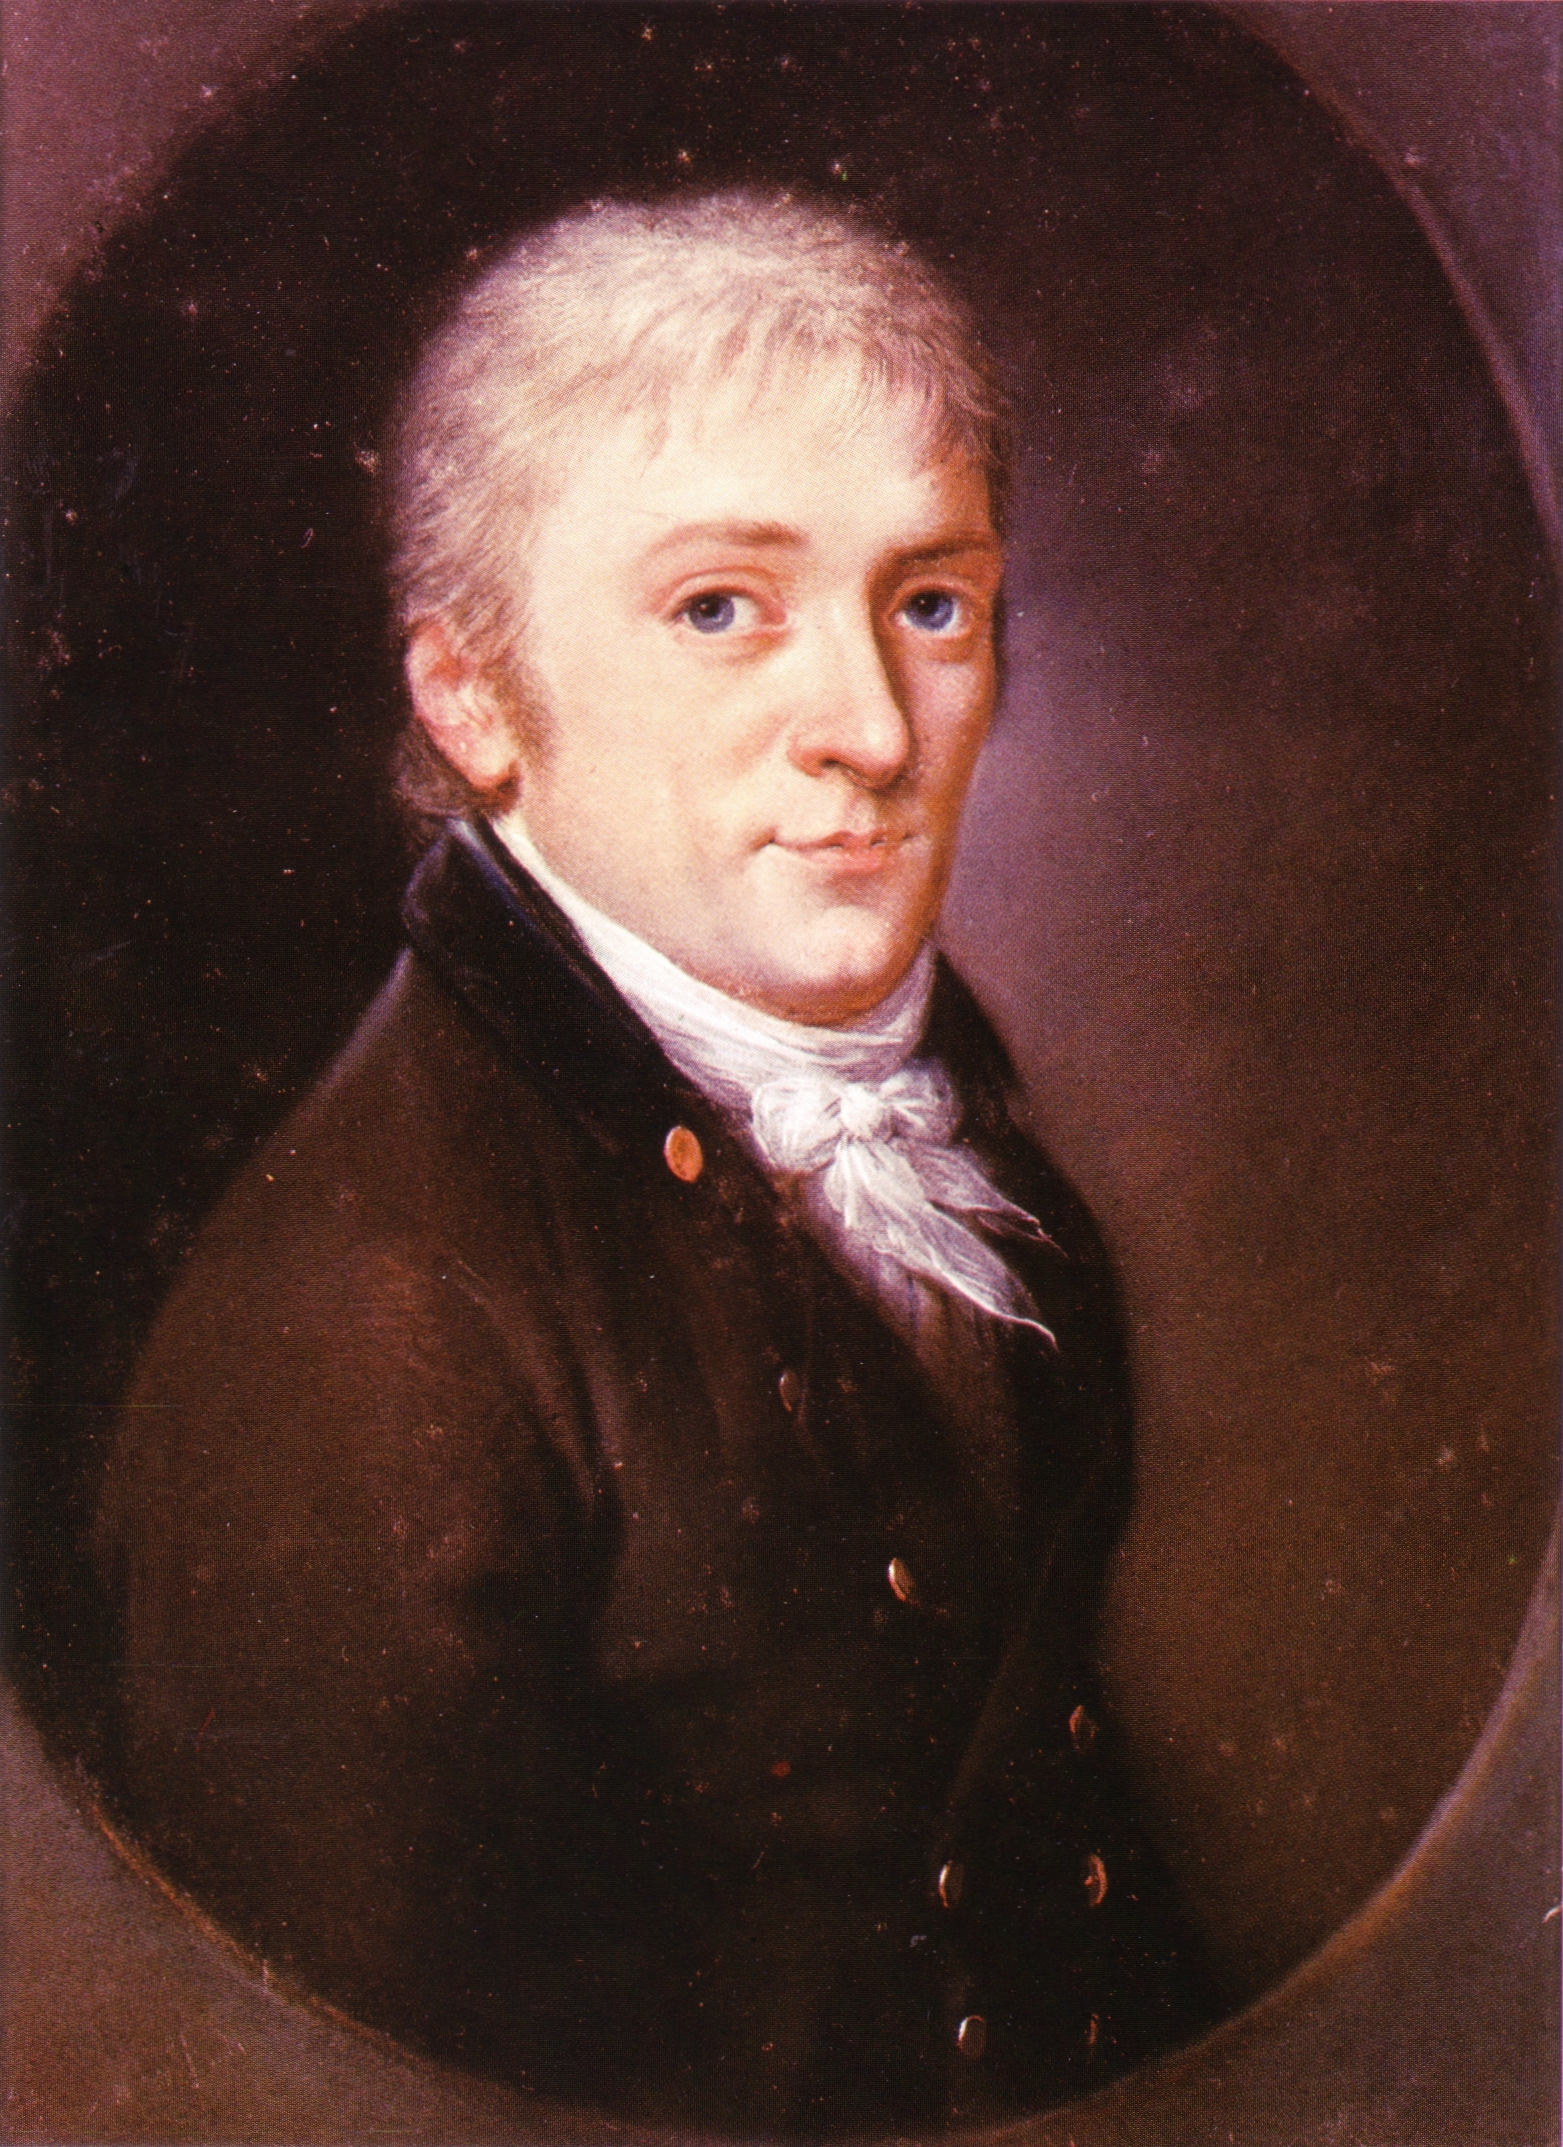
\includegraphics[width=0.32\textwidth]{gauss1803.jpg}%
    };
  \end{tikzpicture}
  \caption[Carl Friedrich Gauss]{\sloppy{Carl Friedrich Gauss. Pastel painting by Johann Christian August Schwartz, 1803.}}
  \label{figure:gauss-1803}
\end{figure}
\zcrefnamed{theorem:wilsons-theorem} can be used to prove a historically important result in the development of modular arithmetic: that $-1$ is congruent to a square modulo an odd prime $p$ if and only if $p\equiv 1\pmod{4}$.
In his \emph{Disquisitiones Arithmeticae} \cite{gauss1986}, Gauss writes of this result that when he encountered it in 1795---he was 19 at the time---he considered it to be a result of rare beauty and suspected deep connections with even
more profound results, that he concentrated all his efforts into understanding its underlying principles. He became so attracted by the questions of this nature, that he could not let them be. Ultimately, Gauss's investigations into higher arithmetic, as he preferred to call it, led him to prove the celebrated \zcrefnamed{theorem:quadratic-reciprocity}.

While the law of quadratic reciprocity is certainly the central theorem of our subject, the quadratic character of $-1$ modulo a prime is a key result on its own. In this section we will show that it can be used to show that there are infinitely many primes congruent to $1$ modulo $4$. Furthermore, we will use the fact that $-1$ is congruent to a square modulo $p$ when $p\equiv 1\pmod{4}$ in the next chapter to prove Fermat's \emph{Two-Square Theorem}, which asserts that every such prime is the sum of two squares. Questions similar to the quadratic character of $-1$ modulo a prime will be investigated more fully in \zcref{chapter:quadratic-residues,chapter:quadratic-reciprocity}.

\begin{theorem}[The Quadratic Character of $-1$]\label{theorem:quadratic-character-neg-1}
  Consider an odd prime $p$. Then there exists an integer $a$ such that
  \begin{equation*}
    a^2\equiv-1\pmod{p}
  \end{equation*}
  if and only if $p\equiv 1\pmod{4}$.
\end{theorem}

\begin{proof}
  First, we show that if there is an integer $a$ such that $a^2\equiv-1\pmod{p}$, then we must have $p\equiv 1\pmod{4}$. By \zcrefnamed{theorem:fermats-little-theorem} it follows that
  \begin{equation*}
    (-1)^{\frac{p-1}{2}}\equiv (a^2)^{\frac{p-1}{2}} \equiv a^{p-1}\equiv 1\pmod{p}
  \end{equation*}
  This shows that $\frac{p-1}{2}$ must be even, which is equivalent to the congruence $p\equiv 1\pmod{4}$.
  
  For the converse, assume that $p\equiv 1\pmod{4}$. By \zcrefnamed{theorem:wilsons-theorem} we know that $(p-1)!\equiv -1\pmod{p}$. Now, observe that the integers $1,\ldots,p-1$ can be arranged in pairs, where each $i$ is paired with $p-i$, which is always distinct from $i$ because $p-1$ is even. Since $i(p-i)\equiv -i^2\pmod{p}$, we obtain the congruences
  \begin{equation*}
    -1\equiv(p-1)!\equiv (-1)^{\frac{p-1}{2}}\left(\left(\frac{p-1}{2}\right)!\right)^2\equiv\left(\left(\frac{p-1}{2}\right)!\right)^2\pmod{p}.
  \end{equation*}
  The last congruence holds, because $(p-1)/2$ is even by the assumption that $p\equiv 1\pmod{4}$. Thus, we have presented $-1$ as a square modulo $p$.
\end{proof}

The previous theorem describing the quadratic character of $-1$ modulo an odd prime $p$ can be used to show that there are infinitely many primes congruent to $1$ modulo $4$. The first fifteen primes congruent to $1$ modulo $4$ are:
\begin{equation*}
  5,~13,~17,~29,~37,~41,~53,~61,~73,~89,~97,~101,~109,~113,~\text{and}~137.
\end{equation*}

\begin{theorem}
  There are infinitely many primes congruent to $1$ modulo $4$.
\end{theorem}

\begin{proof}
  Consider a finite set of primes $p_1,\ldots,p_k$ that are all congruent to $1$ modulo $4$, and define
  \begin{equation*}
    n = (2p_1\cdots p_k)^2 + 1.
  \end{equation*}
  Notice that $n\equiv 1\pmod{4}$ is greater than $1$, and $p_i\nmid n$ for any $1\leq i\leq k$. It follows that for any prime divisor $q$ of $n$, we have
  \begin{equation*}
    (2p_1\cdots p_k)^2\equiv -1\pmod{q},
  \end{equation*}
  showing that $-1$ is a quadratic residue modulo $q$. Since $-1$ is a quadratic residue modulo $q$ if and only if $q\equiv 1\pmod{4}$, it follows that any prime divisor $q$ of $n$ is congruent to $1$ modulo $4$. Since none of the prime divisors of $n$ are among the primes $p_i$ we started out with, the primes $p_i$ could not have listed all the primes congruent to $1$ modulo $4$.
\end{proof}

\zcref{theorem:quadratic-character-neg-1} and its proof can be generalized to arbitrary exponents. For example, the following theorem implies that the congruence $x^4\equiv -1\pmod{p}$ is solvable if and only if $p\equiv 1\pmod{8}$, that the congruence $x^8\equiv -1\pmod{p}$ is solvable if and only if $p\equiv 1\pmod{16}$, and so on.

\begin{theorem}
  Consider an odd prime $p$ and consider a natural number $n$ with $2$-adic decomposition $n=2^km$. Then the congruence
  \begin{equation*}
    x^n \equiv -1\pmod{p}
  \end{equation*}
  is solvable if and only if $p\equiv 1\pmod{2^{k+1}}$.
\end{theorem}

\begin{proof}
  The proof is by induction on $k$. For $k=0$, the statement is trivial, and for $k=1$, the proof was given in \zcref{theorem:quadratic-character-neg-1}. For the inductive step, assume that for any number $n$ with $2$-adic decomposition $n=2^km$, the congruence $x^n\equiv-1\pmod{p}$ is solvable if and only if $p\equiv 1\pmod{2^{k+1}}$, and consider a number $n$ with $2$-adic decomposition $n=2^{k+1}m$.

  For the forward direction, assume that $a$ is an integer such that $a^n\equiv -1\pmod{p}$. Then $b:=a^{2m}$ is an integer such that
  \begin{equation*}
    b^{2^k}\equiv -1\pmod{p},
  \end{equation*}
  so we see that $p\equiv 1\pmod{2^{k+1}}$. Consequently, the fraction
  \begin{equation*}
    \frac{p-1}{2^{k+1}}
  \end{equation*}
  is an integer. By \zcrefnamed{theorem:fermats-little-theorem} it follows that
  \begin{equation*}
    (-1)^{\frac{p-1}{2^{k+1}}}\equiv(a^{2^{k+1}m})^{\frac{p-1}{2^{k+1}}}\equiv (a^m)^{p-1}\equiv 1\pmod{p}.
  \end{equation*}
  This implies that $\frac{p-1}{2^{k+1}}$ is even, so that $p\equiv 1\pmod{2^{k+2}}$.

  For the converse, suppose that $p\equiv 1\pmod{2^{k+2}}$ and consider an integer $a$ such that $a^{2^k}\equiv -1\pmod{p}$. Such an integer exists by the inductive hypothesis. Now partition the set of numbers $\{1,\ldots,p-1\}$ into classes of $2^{k+1}$ numbers of the form $\{x,ax,\ldots,a^{2^{k+1}-1}x\}$. We will write $c$ for the number of such classes. Then we have $p=2^{k+1}c+1$, so we see that $c$ is even.

  Since the number of classes is $c$, we can label them by $C_i$ for each $1\leq i\leq c$, and we can pick a representative $x_i\in C_i$ for each $i$. Now it follows by \zcrefnamed{theorem:wilsons-theorem} that
  \begin{equation*}
    -1\equiv (p-1)!\equiv \prod_{i=1}^c \prod_{j=0}^{2^{k+1}-1} a^jx_i \equiv \prod_{i=1}^c (-1)x_i^{2^{k+1}} \equiv (-1)^c\prod_{i=1}^c x_i^{2^{k+1}} \equiv \left(\prod_{i=1}^c x_i\right)^{2^{k+1}}\pmod{p}.\qedhere
  \end{equation*}
\end{proof}

\section{The Infinitude of Primes Congruent to 1 Modulo Powers of 2}

One way to show that a prime $p$ is congruent to $1$ modulo $n$ is by finding an integer $a$ such that
\begin{equation*}
  \ord_p(a)=n.
\end{equation*}
By \zcrefnamed{theorem:order-theorem} and \zcrefnamed{theorem:fermats-little-theorem}, this implies that $n\mid p-1$. We will use this idea to show that there are infinitely many primes congruent to $1$ modulo any power of $2$. In particular, there are infinitely many primes congruent to $1$ modulo $4$, modulo $8$, modulo $16$, and so on.

\begin{theorem}\label{theorem:infinitude-of-primes-1-mod-power-of-2}
  For any positive natural number $n$, there are infinitely many primes congruent to $1$ modulo $2^n$.
\end{theorem}

\begin{proof}
  Since $p\equiv 1\pmod{2^{n+1}}$ implies that $p\equiv 1\pmod{2^n}$, it suffices to show that for any finite list $p_1,\ldots,p_k$ of primes congruent to $1$ modulo $2^{n+1}$, there is a prime $q\equiv 1\pmod{2^{n+1}}$ which is not among the primes $p_i$.

  Given such a list of primes $p_i$, let
  \begin{equation*}
    a:=2p_1\cdots p_k,
  \end{equation*}
  and let $q$ be a prime divisor of the integer $b:=a^{2^n}+1$. Note that $q$ is necessarily an odd prime, since $a$ is even and hence $b$ is odd. Since $p_i\nmid b$ for any $i$, it follows that $q$ is not among the primes $p_i$. Furthermore, we observe that
  \begin{equation*}
    a^{2^n}\equiv -1\pmod{q}.
  \end{equation*}
  This implies that $\ord_q(a)\mid 2^{n+1}$, while clearly $\ord_q(a)\nmid 2^n$. Thus, we must have $\ord_q(a)=2^{n+1}$, and this allows us to conclude that $q\equiv 1\pmod{2^{n+1}}$.
\end{proof}

The previous theorem is a special case of a deep theorem in analytic number theory: \emph{Dirichlet's Theorem}. Dirichlet's Theorem shows that for any integer $a$ relatively prime to $n$, there are infinitely many primes
\begin{equation*}
  p\equiv a\pmod{n}.
\end{equation*}
The techniques of proving Dirichlet's Theorem are beyond the scope of this course. However, having taken this course, you are well equipped to read LeVeque's excellent \emph{Topics in Number Theory} \cite{leveque1956vol1,leveque1956vol2}, a two-volume work that contains well-explained proofs of Dirichlet's Theorem as well as the Prime Number Theorem.

\exercises

\begin{starter}
  \exercise For every prime $p\equiv 1\pmod{4}$ below $100$, find the least positive integer $a$ such that $a^2\equiv -1\pmod{p}$.
  \exercise
  \begin{subexenum}
  \item Consider two integers $a$ and $b$, and a prime number $p$. Prove, without using Fermat's Little Theorem, that
    \begin{equation*}
      (a+b)^p\equiv a^p+b^p\pmod{p}.
    \end{equation*}
  \item Suppose that $a\geq 0$. Use the previous congruence and the fact that $a=\sum_{i=1}^a1$ to give your own proof of Fermat's Little Theorem.
  \end{subexenum}
  \exercise
  \begin{subexenum}
  \item Prove that
    \begin{equation*}
      5^{5^5}\equiv 5^5\pmod{31}.
    \end{equation*}
  \item Prove that
    \begin{equation*}
      7^{7^7}\equiv 7^7\pmod{43}.
    \end{equation*}
  \end{subexenum}
\end{starter}

\begin{routine}
  \exercise Show that
  \begin{equation*}
    2^{p-2}+3^{p-2}+6^{p-2} \equiv 1 \pmod{p}
  \end{equation*}
  for any prime number $p\neq 3$.
  \exercise For any positive integer $n$ we define the \emph{Euler quotient}
  \begin{equation*}
    q_n(x):=\frac{x^{\phi(n)}-1}{n},
  \end{equation*}
  where $x$ is assumed to be relatively prime to $n$. In the special case where $n$ is a prime, $q_n(x)$ is called the \emph{Fermat quotient}.
  \begin{subexenum}
  \item Show that
    \begin{equation*}
      q_n(ab)\equiv q_n(a)+q_n(b)\pmod{n}
    \end{equation*}
    for any two integers $a$ and $b$ relatively prime to $n$, and conclude that $q_n(a^k)\equiv k q_n(a)\pmod{n}$ for $a$ relatively prime to $n$.
  \item For any prime $p$, define the \emph{Wilson quotient} $W_p$ by
    \begin{equation*}
      W_p:=\frac{(p-1)!+1}{p}.
    \end{equation*}
    Prove \emph{Lerch's formula} \cite{lerch1905}, which asserts that
    \begin{equation*}
      \sum_{k=1}^{p-1}q_p(k)\equiv W_p\pmod{p}.
    \end{equation*}
  \end{subexenum}
  \exercise Show that
  \begin{equation*}
    3^{3^{3^3}}\equiv 3^{3^3}\pmod{97}.
  \end{equation*}
  \exercise
  \begin{subexenum}
  \item Show that any number of the form
    \begin{equation*}
      m^5n-n^5m
    \end{equation*}
    is divisible by $30$.
  \item Show that for any two odd primes $p$ and $q$, the number
    \begin{equation*}
      p^5q-q^5p
    \end{equation*}
    is divisible by $240$.
  \end{subexenum}
  \exercise Prove that if
  \begin{equation*}
    a^n\equiv a \pmod{n}
  \end{equation*}
  for every integer $a$, then $n=2$ or $n$ is odd.
  \exercise Consider two distinct primes $p$ and $q$, and an integer $a\geq 0$. Prove that
  \begin{equation*}
    a^{pq}+a\equiv a^p + a^q \pmod{pq}
  \end{equation*}
  \exercise Consider an odd prime $p=2n+1$. Show that
  \begin{equation*}
    \binom{2n}{n}\equiv (-1)^{\frac{p-1}{2}}\pmod{p}.
  \end{equation*}
  \exercise Consider a prime $p$ and two numbers $m$ and $n$. Prove that
  \begin{equation*}
    \binom{p^kn}{p^km}\equiv \binom{n}{m}\pmod{p}.
  \end{equation*}
  \exercise Show that the congruence
  \begin{equation*}
    \sum_{k=1}^{n} k^n\equiv 0\pmod{n}
  \end{equation*}
  holds if and only if $n$ is odd.
  \exercise
  \begin{subexenum}
  \item Consider a prime $p$ and an integer $p\nmid a$. Show that
    \begin{equation*}
      a^p\equiv a\pmod{p^2}\qquad\Leftrightarrow \qquad a^{p^2}\equiv a\pmod{p^2}.
    \end{equation*}
  \item A prime satisfying $a^p\equiv a\pmod{p^2}$ is called a \emph{Wieferich prime base $a$}. Wieferich encountered this condition by showing that if $x^p+y^p=z^p$ with $p\nmid xyz$, then $p$ must be a Wieferich prime base $2$ \cite{wieferich1909}. The only known Wieferich primes base $2$ are $p=1093$ and $p=3511$, and there are no smaller Wieferich primes base $2$.
    
    In bases larger than $2$ there are smaller Wieferich primes, although they are still rare. The only known Wieferich primes base $3$ are $p=11$ and $p=1006003$. Show that $5$ is a Wieferich prime base $32$.
  \end{subexenum}
\end{routine}

\begin{challenge}
  \exercise Find the least integer $k>1$ such that every integer of the form $x^k-x$ is divisible by $47$ and $89$.
  \exercise Find a prime $p>3$ such that
  \begin{equation*}
    3^{3^3}\equiv 3^3\pmod{p}.
  \end{equation*}
  \exercise For any integer $a$ and any prime number $p$, show that
  \begin{equation*}
    a^{p^k} \equiv a^{p^{k-1}} \pmod{p^k}.
  \end{equation*}
  \exercise Find all the solutions to the equation
  \begin{equation*}
    p^q-q^p=p+q,
  \end{equation*}
  where $p$ and $q$ are prime numbers.
  \exercise Consider two primes $p$ and $q$. Show that
  \begin{equation*}
    pq\mid (13^p-5^p)(13^q-5^q)\qquad\Leftrightarrow\qquad pq\mid 12.
  \end{equation*}
  \exercise
  \begin{subexenum}
  \item Show that the number $6481=3^8-3^4+1$ is prime. Hint: In order to avoid trying out all the primes below $80$, show first that every prime factor $p$ of $6481$ satisfies $p\equiv 1\pmod{24}$.
  \item Compute the prime factorization of the number
    \begin{equation*}
      3^{24}-1.
    \end{equation*}
  \end{subexenum}
  \exercise Consider the function $f(n)=2n+1$. Show for every prime $p$, the sequence
  \begin{equation*}
    k\mapsto f^k(p)
  \end{equation*}
  obtained by iterating the function $f$, contains composite numbers.
  \exercise \label{exercise:prime-divisors-feit-thompson-conjecture}
  \begin{subexenum}
  \item Consider an odd prime $q$. Show that the numbers
    \begin{equation*}
      2^q-1 \qquad\text{and}\qquad q+1.
    \end{equation*}
    are relatively prime.
  \item Consider two distinct primes $p$ and $q$, and let $r$ be a common prime divisor of the numbers
  \begin{equation*}
    \frac{p^q-1}{p-1}\qquad\text{and}\qquad\frac{q^p-1}{q-1}.
  \end{equation*}
  Show that $r\equiv 1\pmod{2pq}$.  
  \end{subexenum}
\end{challenge}

%%% Local Variables:
%%% mode: latex
%%% TeX-master: "elementary-number-theory"
%%% TeX-engine: luatex
%%% End:


\chapter{Sums of Squares}

\section{Fermat's Two-Square Theorem}

\begin{theorem}[Fermat's Two-Square Theorem]
  A natural number $n$ is presentable as the sum of two squares if and only if its square-free part is a product of primes congruent to $1$ modulo $4$.
\end{theorem}

\section{Lagrange's Four-Square Theorem}

\begin{theorem}[Lagrange's Four-Square Theorem]
  Every natural number can be written as the sum of four squares.
\end{theorem}

\section{Legendre's Three-Square Theorem}

Characterizing precisely those numbers that can be written as a sum of three squares is harder than the cases for two or four squares, since the numbers expressible as sums of three squares are not closed under multiplication. For example, $3=1^2+1^2+1^2$ and $5=2^2+1^2+0^2$, while $15$ cannot be written as a sum of three squares.

\begin{theorem}[Legendre's Three-Square Theorem]
  A natural number $n$ is presentable as the sum of three squares if and only if it is not of the form $4^k m$ where $m\equiv 7\pmod{8}$.
\end{theorem}


%%% Local Variables:
%%% mode: latex
%%% TeX-master: "elementary-number-theory"
%%% End:



\chapter{The Gaussian Integers}
\label{chapter:gaussian-integers}

\section{Definition and Basic Properties of the Gaussian Integers}

\begin{figure}[t]
  \centering
  \begin{tikzpicture}[scale=1,line join=round,line cap=round]
    
    \draw[->] (-6.5,0) -- (6.5,0) node[right] {$a$};
    \draw[->] (0,-3.5) -- (0,5.5) node[above] {$b$};

    \fill[YellowOrange,opacity=.4] (0,0) -- (3,1) -- (2,4) -- (-1,3) -- cycle;

    \foreach \x in {-6,-5,-4,-3,-2,-1,0,1,2,3,4,5,6} {
      \foreach \y in {-3,-2,-1,0,1,2,3,4,5} {
        \draw[CornflowerBlue,fill=white,thick] (\x,\y) circle (2pt);
      }
    }

    \draw[CornflowerBlue,fill=CornflowerBlue,thick] (-6,-2) circle (2pt);
    \draw[CornflowerBlue,fill=CornflowerBlue,thick] (-3,-1) circle (2pt);
    \draw[CornflowerBlue,fill=CornflowerBlue,thick] (0,0) circle (2pt);
    \draw[CornflowerBlue,fill=CornflowerBlue,thick] (3,1) circle (2pt);
    \node[xshift=2ex,yshift=-2ex] at (3,1) {$3+i$};
    \draw[CornflowerBlue,fill=CornflowerBlue,thick] (6,2) circle (2pt);
    \draw[CornflowerBlue,fill=CornflowerBlue,thick] (-4,2) circle (2pt);
    \draw[CornflowerBlue,fill=CornflowerBlue,thick] (-1,3) circle (2pt);
    \draw[CornflowerBlue,fill=CornflowerBlue,thick] (2,4) circle (2pt);
    \draw[CornflowerBlue,fill=CornflowerBlue,thick] (5,5) circle (2pt);
    \draw[CornflowerBlue,fill=CornflowerBlue,thick] (4,-2) circle (2pt);
    \draw[CornflowerBlue,fill=CornflowerBlue,thick] (1,-3) circle (2pt);
    \draw[CornflowerBlue,fill=CornflowerBlue,thick] (-5,5) circle (2pt);
  \end{tikzpicture}
  \caption[The Gaussian integers]{\label{figure:gaussian-integers}The set of Gaussian integers. All the multiples of $3+i$ are marked with solid dots, and all the nonmultiples are marked with open dots. The norm of $3+i$ is the area of the square shaded in orange.}
\end{figure}

\begin{definition}
  A \define{Gaussian integer} is an expression of the form
  \begin{equation*}
    a+bi
  \end{equation*}
  in which $a$ and $b$ are integers. We say that the \define{real part} of $a+bi$ is the integer $a$, and the \define{complex part} of $a+bi$ is the integer $b$.

  We will write $\mathbb{Z}[i]$ for the set of Gaussian integers. Gaussian integers are added, subtracted, and multiplied according to the following rules:
  \begin{align*}
    (a+ib)+(c+id) & = (a+c)+i(b+d) \\
    (a+ib)-(c+id) & = (a-c)+i(b-d) \\
    (a+ib)(c+id)  & = (ac-bd)+i(ad+bc).
  \end{align*}
\end{definition}

\begin{definition}
  The \define{norm} of a Gaussian integer $\alpha=a+bi$ is given by
  \begin{equation*}
    N(\alpha)=a^2+b^2.
  \end{equation*}
\end{definition}

\begin{proposition}[The Brahmagupta--Fibonacci identity]
  The norm function $N$ is completely multiplicative in the sense that
  \begin{equation*}
    N(\alpha\beta)=N(\alpha)N(\beta)
  \end{equation*}
  for any two Gaussian integers $\alpha$ and $\beta$.
\end{proposition}

\begin{definition}
  A Gaussian integer $\alpha$ is said to \define{divide} a Gaussian integer $\beta$ if there exists a Gaussian integer $\kappa$ such that
  \begin{equation*}
    \kappa\alpha=\beta.
  \end{equation*}
  Any Gaussian integer dividing $1$ is called a \define{unit}.
\end{definition}

\begin{theorem}
  The only units among the Gaussian integers are $\pm 1$ and $\pm i$.
\end{theorem}

\section{Euclidean Division of Gaussian Integers}

\begin{example}
  The following choices of $\alpha$ and $\beta$ show that there can be multiple pairs of Gaussian integers $\kappa$ and $\rho$ with $N(\rho)<N(\beta)$ such that
  \begin{equation*}
    \alpha=\kappa\beta+\rho.
  \end{equation*}
  \begin{enumerate}
  \item Consider $\alpha := 8+11i$ and $\beta=3+i$, so that $N(\beta)=10$. Then
    \begin{equation*}
      \frac{\alpha}{\beta}=\frac{(8+11i)(3-i)}{3^2+1^2}=\frac{35+25i}{10}=(3+2i)+\frac{1+i}{2}.
    \end{equation*}
    This shows that $\alpha = (3+2i)\beta + (1+2i)$. Note that $N(1+2i)=5<10$. However, we can also write
    \begin{align*}
      \alpha & = (4+2i)\beta + (-2+i), & N(-2+i) & = 5,\\
      \alpha & = (3+3i)\beta + (2-i), & N(2-i) & = 5, \\
      \alpha & = (4+3i)\beta + (-2-i), & N(-2-i) & = 5.
    \end{align*}
  \item Consider $\alpha := 2+3i$ and $\beta=4$, so that $N(\beta)=16$. Then we can write
    \begin{align*}
      \alpha & = i\beta + (2-i), & N(2-i) & = 5, \\
      \alpha & = (1+i)\beta + (-2-i), & N(-2-i) & = 5.
    \end{align*}
  \end{enumerate}
\end{example}

Define the half-open fundamental square to be the following subset of $\mathbb{C}$:
\begin{equation*}
  \mathcal{S}:=\big\{x+yi\in\mathbb{C}\mid -\tfrac{1}{2}<x,y\leq \tfrac{1}{2}\big\}.
\end{equation*}

\begin{theorem}
  Consider two Gaussian integers $\alpha$ and $\beta$ with $N(\alpha)>N(\beta)$. Then there exist unique Gaussian integers $\kappa$ and $\rho$ with $N(\rho)<N(\beta)$, such that
  \begin{equation*}
    \alpha=\kappa\beta+\rho
  \end{equation*}
  and $\frac{\rho}{\beta}\in\mathcal{S}$.
\end{theorem}

\section{The Greatest Common Divisor of Gaussian Integers}

The definition of a greatest common divisor carries over directly from the integers to the Gaussian integers.

\begin{definition}
  Consider two Gaussian integers $\alpha$ and $\beta$. A Gaussian integer $\delta$ is said to be the \define{greatest common divisor} of $\alpha$ and $\beta$ if it satisfies the following logical equivalence for every Gaussian integer $\xi$:
  \begin{equation*}
    (\xi\mid \alpha)\land (\xi\mid\beta) \Leftrightarrow (\xi\mid\delta).
  \end{equation*}
\end{definition}

\section{Primes in the Gaussian Integers}

\section{Fermat's Two-Square Theorem}

\section{The Biquadratic Character of \texorpdfstring{$-1$}{-1}}

\exercises

\begin{challenge}
  \exercise
  \begin{subexenum}
  \item Consider a Gaussian integer $\alpha=a+bi$ such that $\gcd(a,b)=1$. Show that the number of Gaussian integers in the interior (that is, not on the boundary) of the square spanned by the Gaussian integers $0$, $\alpha$, $i\alpha$, and $(1+i)\alpha$ is $N(\alpha)-1$. See \zcref{figure:gaussian-integers} for such a square with $\alpha=3+i$.
  \item For any Gaussian integer $\alpha=a+bi$, determine the number of Gaussian integers in the interior of the square spanned by the Gaussian integers $0$, $\alpha$, $i\alpha$, and $(1+i)\alpha$.
    % # Interior points = N(\alpha) - 2\gcd(|a|,|b|) + 1.
  \end{subexenum}
\end{challenge}

%%% Local Variables:
%%% mode: latex
%%% TeX-master: "elementary-number-theory"
%%% TeX-engine: luatex
%%% End:


\chapter{Polynomials}\label{chapter:polynomials}

\section{Polynomials with Abstract Coefficients}

\begin{definition}
  An \emph{polynomial} in one variable $x$ is an expression of the form
  \begin{equation*}
    f(x) = a_nx^n+ a_{n-1}x^{n-1} +\cdots + a_0,
  \end{equation*}
  in which we require that the \emph{leading coefficient} $a_n$ is nonzero, unless $n=0$. A polynomial $f(x)$ as above with leading coefficient $a_n$ is said to be of \emph{degree} $n$. The numbers $a_k$ are called the \emph{coefficients} of $f(x)$. The \emph{zero polynomial} is the constant polynomial $f(x)=0$.
\end{definition}

The coefficients of a polynomial may be taken from any number system. When we wish to specify that the coefficients are integers, rational, or real numbers, we speak of \emph{polynomials with integer coefficients}, \emph{polynomials with rational coefficients}, or \emph{polynomials with real coefficients}. Other number systems from which we will occasionally take coefficients include the rings $\mathbb{Z}/n$ of modular arithmetic. Since there is such a large variety of number systems which will eventually play a role one way or another in number theory, it will be useful to us to develop methods general enough so as to cover all these cases at once.

\begin{definition}
  A \emph{commutative ring} is a set $R$ equipped with constants $0$ and $1$ and operations $+$ for addition, $-$ for subtraction, and $\cdot$ for multiplication, satisfying the following laws of arithmetic:
  \begin{align*}
    (x+y)+z & = x + (y+ z), & (xy)z & = x(yz), \\
    x + y & = y + x, & xy & = yx, \\
    0+x & = x, & 1x & = x, \\
    x+(-x) & = 0, & x(y+z) & = xy+xz.
  \end{align*}
  The adjective \emph{commutative} refers to the law asserting that $xy=yx$. A commutative ring with $0\neq 1$ is said to be a \emph{integral domain} if it satisfies the following condition:
  \begin{equation*}
    xy=0 \Rightarrow x=0\lor y=0.
  \end{equation*}
  A commutative ring with $0\neq 1$ is said to be a \emph{field} if it comes equipped with a further operation $({-})^{-1}$ defined on all nonzero elements, such that
  \begin{equation*}
    xx^{-1}=1.
  \end{equation*}
\end{definition}

Examples of commutative rings include most number systems we have encountered so far: $\mathbb{Z}$, $\mathbb{Q}$, and $\mathbb{Z}/n$ for any $n$. The Gaussian integers $\mathbb{Z}[i]$ are another important example of a ring. There is one important omission: The set of natural numbers with the usual operations of addition and multiplication is not a ring because it lacks subtraction.

The sharp reader may have observed that some laws of arithmetic, such as $0x=0$, are not stated in the definition of a (commutative) ring. Indeed, this law can be proven:
\begin{equation*}
  0x=0x+0=0x+(0x-0x)=(0x+0x)-0x=(0+0)x-0x=0x-0x=0.
\end{equation*}
Most rings satisfy the condition that $0\neq 1$. Indeed, if $0=1$ in a ring $R$, then any element equals $0$ because
\begin{equation*}
  x=1x=0x=0.
\end{equation*}
Thus, only the ring $\mathbb{Z}/1$ satisfies $0=1$. This ring is called the \emph{trivial ring} for understandable reasons.

The condition of being an integral domain is quite innocent-looking: It guarantees that the product of any two nonzero numbers is nonzero. This condition is true in familiar number systems such as $\mathbb{Z}$, $\mathbb{Z}[i]$, $\mathbb{Q}$, and $\mathbb{R}$, which are therefore integral domains. However, the ring $\mathbb{Z}/n$ is only an integral domain when $n$ is prime. For composite $n$, we can find examples of nonzero numbers that multiply to $0$. For instance, we have $2\cdot 2\equiv 0\pmod{4}$ in $\mathbb{Z}/4$, and we have $2\cdot 3\equiv 0\pmod{6}$ in $\mathbb{Z}/6$. Having such examples shows that the condition of being an integral domain is not provable from the laws of arithmetic stated in the definition of a ring.

Of the examples we have seen so far, only $\mathbb{Q}$ and $\mathbb{Z}/p$ are fields. Other familiar fields include the field $\mathbb{R}$ of real numbers and the field $\mathbb{C}$ of complex numbers. We note that any field is an integral domain: If $xy=0$ and $x\neq 0$, then $x$ has a multiplicative inverse. This allows us to calculate as follows and find that
\begin{equation*}
  y=1y=(x^{-1}x)y=x^{-1}(xy)=x^{-1}0=0.
\end{equation*}

The previous definitions of rings, integral domains, and fields are extremely general. There are many examples of rings that have little to do with numbers, except that they satisfy the laws of arithmetic. We stress here that our goal is not to develop the general theory of rings, where we would have to be concerned with the vast scope of the subject. Instead, our goal is simply to avoid having to reprove essentially the same theorems about polynomials separately for polynomials with integer coefficients, rational coefficients, real coefficients, and so on. By stating them in terms of polynomials with coefficients in a ring or integral domain, we cover all those cases at once.

\begin{remark}
  There is another subtle, yet important aspect of polynomials which needs to be emphasized: The distinction between polynomials and the functions they describe. This distinction comes to light when considering equality of polynomials. Two polynomials
  \begin{equation*}
    a_nx^n+ a_{n-1}x^{n-1} +\cdots + a_0\qquad\text{and}\qquad b_nx^n+ b_{n-1}x^{n-1} +\cdots + b_0
  \end{equation*}
  are said to be equal if their coefficients are equal, meaning that $a_i=b_i$ for all $0\leq i\leq n$, while functions are considered equal if their values are equal. This is an important distinction, because for some number systems such as the integers modulo $n$, polynomials aren't necessarily equal as polynomials when they are equal as functions. For instance, by \crefnamed{theorem:fermats-little-theorem} we have that
  \begin{equation*}
    x^p \equiv x\pmod{p},
  \end{equation*}
  while the polynomials $x^p$ and $x$ clearly can be distinguished by their coefficients. Nevertheless, we will show in \cref{corollary:extensionality-integer-polynomials} that two polynomials with integer coefficients have equal coefficients if and only if they define equal functions.
\end{remark}

\begin{definition}
  Consider a ring $R$. A function $f:R\to R$ is said to be \emph{polynomial in $R$} if there exists a polynomial with coefficients in $R$ such as the above, such that
  \begin{equation*}
    f(x)=a_nx^n+ a_{n-1}x^{n-1} +\cdots + a_0
  \end{equation*}
  for all $x\in R$.
\end{definition}

\begin{remark}
  Polynomials can be added, subtracted, and multiplied in the same way as integers. To add two polynomials, we add their corresponding coefficients, taking missing coefficients as zero when necessary. Polynomials are multiplied by the formula
  \begin{align*}
    \Biggl(\sum_{i=0}^n a_ix^i\Biggr)\Biggl(\sum_{j=0\vphantom{i=0}}^mb_jx^j\Biggr)
    & = \sum_{i=0}^n\sum_{j=0}^ma_ib_jx^{i+j} \\
    & = \sum_{k=0}^{n+m}\sum_{i=0}^n a_i b_{k-i}x^{k}.    
  \end{align*}
  These operations of addition, subtraction, and multiplication of polynomials satisfy the laws of arithmetic. More precisely, the polynomials with coefficients in a commutative ring form itself a commutative ring.
\end{remark}

\section{The Factor Theorem}

\begin{definition}
  Consider a polynomial $f(x)$ with coefficients in a ring $R$. A \emph{root} of $f(x)$ is an element $r\in R$ such that
  \begin{equation*}
    f(r)=0.
  \end{equation*}
  Sometimes we will write $N(f)$ for the set of roots of $f$.
\end{definition}

In the following theorem we will prove that if $r$ is a root of the polynomial $f(x)$, then we can factor $f(x)$ as $(x-r)g(x)$. This theorem applies for polynomials in any commutative ring.

\begin{theorem}[Factor Theorem]\label{theorem:factor-theorem}
  Consider a ring $R$, and a nonzero polynomial $f(x)$ of degree $n$ with coefficients in $R$.
  An element $r\in R$ is a root of $f(x)$ if and only if there is a polynomial $g(x)$ of degree $n-1$ with coefficients in $R$ such that $f(x)=(x-r)g(x)$.
\end{theorem}

\begin{proof}
  We will prove the claim by induction on $n$. In the base case $f(x)$ is a nonzero constant polynomial, so it has no roots and there is nothing to prove.

  For the inductive step, it is clear that if there is a polynomial $g(x)$ such that $f(x)=(x-r)g(x)$, then $r$ is a root of the polynomial $f(x)$. For the converse, suppose that $r$ is a root of $f(x)$. Then
  \begin{equation*}
    f(x) = f(x)-f(r) = a_n(x^n-r^n)+\cdots + a_1(x-r).
  \end{equation*}
  By the formula for the difference of $k$th powers, which was stated in \cref{exercise:difference-of-powers} and which holds in any ring, we can factor $x^k-r^k$ as
  \begin{equation*}
    x^k-r^k=(x-r)q_k(x),\qquad\text{where}\qquad q_k(x)=\sum_{i=0}^{k-1}x^ir^{k-1-i}
  \end{equation*}
  is a polynomial of degree $k-1$. Now define $g(x) := \sum_{k=1}^{n}a_k q_k(x)$. Then we compute
  \begin{equation*}
    (x-r)g(x)=\sum_{k=1}^{n}a_k (x-r)q_k(x)=\sum_{k=1}^{n}a_k (x^k-r^k)=f(x)-f(r)=f(x).\qedhere
  \end{equation*}
\end{proof}

\crefnamed{theorem:factor-theorem} has some important corollaries. One of them states that in an integral domain, where the product of any two nonzero numbers is guaranteed to be nonzero, any polynomial of degree $n$ has at most $n$ roots.

\begin{corollary}\label{corollary:number-of-roots-polynomial}
  Consider an integral domain $R$. A polynomial of degree $n$ with coefficients in $R$ has at most $n$ roots.
\end{corollary}

\begin{proof}
  The proof is by induction on the degree $n$. If $f(x)$ is a constant polynomial of degree $0$ and its leading coefficient is nonzero, then $f(x)$ is always nonzero and so $f(x)$ has no roots.

  For the inductive step, assume that all polynomials of degree $n$ have at most $n$ roots, and consider a polynomial $f(x)$ of degree $n+1$. Then either $f(x)$ has no roots, in which case we are done immediately, or $f(x)$ has a root $r$, in which case $f(x)$ factors as
  \begin{equation*}
    f(x)=(x-r)g(x)
  \end{equation*}
  by \crefnamed{theorem:factor-theorem}, where $g(x)$ is a polynomial of degree $n$. Since we assumed that $R$ is an integral domain, it follows that for any element $x\in R$, the identity $(x-r)g(x)=0$ holds in $R$ if and only if one of the identities $x-r=0$ or $g(x)=0$ holds in $R$. Thus we see that $x$ is a root of the polynomial $f(x)$ if and only if $x=r$ or $x$ is a root of the polynomial $g(x)$. We conclude that the polynomial $f(x)$ has at most $n+1$ roots.
\end{proof}

The Factor Theorem also raises an immediate question of uniqueness. If $f(x)$ and $g(x)$ are two polynomials, is there always at most one way in which we can write
\begin{equation*}
  f(x)=g(x)h(x)?
\end{equation*}

\begin{proposition}[Cancellation Law for Polynomials]\label{proposition:cancellation-law-polynomials}
  Let $f(x)$ be a nonzero polynomial with coefficients in an integral domain. Consider two polynomials $h(x)$ and $k(x)$ satisfying the identity of polynomials
  \begin{equation*}
    f(x)h(x)=f(x)k(x).
  \end{equation*}
  Then $h(x)=k(x)$. 
\end{proposition}

\begin{proof}
  By the assumption that $f(x)h(x)=f(x)k(x)$, it follows that
  \begin{equation*}
    f(x)(h(x)-k(x))=0.
  \end{equation*}
  Write $g(x):=h(x)-k(x)$. Note that all the coefficients of the polynomial $f(x)g(x)$ are $0$. However $f(x)$ is a nonzero polynomial, so it has a leading coefficient $a_n$. Now, suppose for a contradiction that $g(x)$ is nonzero, with leading coefficient $b_m$. Their product $f(x)g(x)$ has leading coefficient $a_nb_m$, which is nonzero since it is a product of nonzero elements of an integral domain. Hence $f(x)g(x)$ is nonzero, which is a contradiction.
\end{proof}

\section{Polynomial Congruences of Prime Moduli}

Even though a polynomial
\begin{equation*}
  f(x) = a_nx^n+ a_{n-1}x^{n-1} +\cdots + a_0
\end{equation*}
has at most $n$ roots in the integers, the same is not true in modular arithmetic. A fairly easy example, the quadratic congruence
\begin{equation*}
  x^2 \equiv 1\pmod{8}
\end{equation*}
has four solutions, the numbers $1$, $3$, $5$, and $7$. On the other hand, we will prove in this section that the number of solutions of a polynomial congruence modulo a prime is, just as in the integer case, at most the degree of the polynomial.

\begin{theorem}[Factor Theorem in Modular Arithmetic]\label{theorem:factor-theorem-modular-arithmetic}
  An integer $r$ is a solution to the polynomial congruence
  \begin{equation*}
    f(x) \equiv 0\pmod{n},
  \end{equation*}
  if and only if
  \begin{equation*}
    f(x) \equiv (x-r)g(x) \pmod{n}
  \end{equation*}
  for some polynomial $g(x)$.
\end{theorem}

\begin{proof}
  The proof is very similar to the proof of \cref{theorem:factor-theorem}. First, we note that the converse direction is trivial, so we focus on the forward direction. Suppose that
  \begin{equation*}
    f(r) \equiv 0 \pmod{n}
  \end{equation*}
  and consider the polynomial $f(x)-f(r)$. Then we have
  \begin{equation*}
    f(x)\equiv f(x)-f(r) \pmod{n},
  \end{equation*}
  and the factorization of $f(x)-f(r)$ as $(x-r)g(x)$ follows in the same way as for \cref{theorem:factor-theorem}.
\end{proof}

\begin{theorem}[Lagrange's Theorem]\label{theorem:lagranges-theorem}
  Consider a polynomial
  \begin{equation*}
    f(x) = a_nx^n+ a_{n-1}x^{n-1} +\cdots + a_0,
  \end{equation*}
  and a prime $p$ such that $p\nmid a_n$. Then the polynomial congruence
  \begin{equation*}
    f(x)\equiv 0 \pmod{p}
  \end{equation*}
  has at most $n$ solutions.
\end{theorem}

\begin{proof}
  We prove the claim by induction on the degree $n$ of the polynomial $f$. If $f$ has degree zero, then $f(x)=a_0$, and since the leading term of $f$ is assumed to be not divisible by $p$, it follows that $a_0\nequiv 0\pmod{p}$. Thus, the polynomial $f$ has no solutions modulo $p$.

  Now suppose that any polynomial congruence modulo $p$ of degree $n$ has at most $n$ solutions, and consider a polynomial congruence $f(x)\equiv 0\pmod{p}$ of degree $n+1$. If this congruence has no roots, then the number of solutions is certainly below $n+1$.

  On the other hand, if $f(r)\equiv 0\pmod{p}$ is a solution, then by \crefnamed{theorem:factor-theorem-modular-arithmetic} we can find a polynomial $g(x)$ of degree $n$ such that
  \begin{equation*}
    f(x)\equiv (x-r)g(x) \pmod{p}.
  \end{equation*}
  It follows that the polynomial congruences $f(x)\equiv 0\pmod{p}$ and
  \begin{equation*}
    (x-r)g(x)\equiv 0 \pmod{p}
  \end{equation*}
  have the same sets of solutions. Since $p$ is prime, we have by \cref{proposition:euclid-divisibility-primes} that $ab\equiv 0\pmod{p}$ if and only if $a\equiv 0\pmod{p}$ or $b\equiv 0\pmod{p}$. Any solution $x$ of the congruence $(x-r)g(x)\equiv 0\pmod{p}$ must therefore satisfy $x-r\equiv 0\pmod{p}$ or $g(x)\equiv 0\pmod{p}$. There are at most $d$ solutions of the polynomial congruence $g(x)\equiv 0\pmod{p}$, so we conclude that there are at most $d+1$ solutions to the polynomial congruence $f(x)\equiv 0\pmod{p}$.
\end{proof}

The previous theorem is due to Joseph-Louis Lagrange, published in 1770 in \emph{Réflexions sur la résolution algébrique des équations} \cite{lagrange1770}. Lagrange demonstrated that the roots of polynomials can be studied by their permutations. His ideas would eventually lead to the emergence of group theory (the study of symmetry), and Galois theory.

While \crefnamed{theorem:lagranges-theorem} establishes an upper bound for the number of incongruent solutions of a polynomial congruence modulo a prime, we can use \crefnamed{theorem:fermats-little-theorem} to find examples of polynomial congruences that have the maximum allowable number of solutions.

\begin{theorem}\label{theorem:maximal-number-of-roots-pow-minus-id}
  Consider a prime $p$ and a positive integer $n$ such that $n\mid p-1$. Then the polynomial congruence
  \begin{equation*}
    x^n\equiv 1\pmod{p}
  \end{equation*}
  has exactly $n$ incongruent solutions.
\end{theorem}

\begin{proof}
  Note that the polynomial congruence $x^{p-1}-1\equiv 0\pmod{p}$ has exactly $p-1$ solutions. By the formula for the difference of powers, we have
  \begin{equation*}
    (x^{p-1}-1)\equiv (x^n-1)q(x) \pmod{p}
  \end{equation*}
  for some polynomial $q$ of degree $p-1-n$. Now we observe that the polynomial congruences
  \begin{equation*}
    x^n-1\equiv 0\pmod{p}\qquad\text{and}\qquad q(x)\equiv 0\pmod{p}
  \end{equation*}
  have at most $n$ and $p-1-n$ solutions, respectively. Since their product has $p-1$ solutions, it follows that the polynomial congruence $x^n-1\equiv 0\pmod{p}$ must have exactly $n$ solutions.
\end{proof}

\crefnamed{theorem:lagranges-theorem} can also be used to give another proof of \cref{theorem:quadratic-character-neg-1}, which states that for an odd prime $p$, the quadratic congruence $x^2\equiv -1\pmod{p}$ has a solution if and only if $p\equiv 1\pmod{4}$.

\begin{proof}[Proof of \cref{theorem:quadratic-character-neg-1}]
  We prove that if $p\equiv 1\pmod{4}$, then there is a square root of $-1$ modulo $p$. Consider a prime $p$ of the form $4k+1$. Then \crefnamed{theorem:fermats-little-theorem} implies that
  \begin{equation*}
    (x^{2k}+1)(x^{2k}-1)=x^{4k}-1\equiv 0\pmod{p}.
  \end{equation*}
  Since $p$ is prime, this implies that $x^{2k}+1\equiv 0\pmod{p}$ or $x^{2k}-1\equiv 0\pmod{p}$ for every integer $x$. However, the polynomial congruence
  \begin{equation*}
    x^{2k}-1\equiv 0\pmod{p}
  \end{equation*}
  has at most $2k$ solutions modulo $p$, which is strictly fewer than $p$. Thus, there must exist an integer $x$ such that
  \begin{equation*}
    x^{2k}+1\equiv 0\pmod{p}.
  \end{equation*}
  Given such an integer $x$, we see that $y:=x^k$ is a square root of $-1$ modulo $p$.
\end{proof}

\section{Lagrange's Interpolation Theorem}

Lagrange's Interpolation Theorem establishes that for any set of data points, as illustrated in \cref{figure:lagrange-interpolation}, there is always a way of defining a polynomial that exactly matches the data. Moreover, it gives the unique way of defining such a polynomial in the lowest degree. Interpolation theorems such as Lagrange's or Newton's addressed a practical need for geometers of the $17th$ and $18th$ centuries: It allowed them to estimate intermediate values of a function from a finite amount of data such as tables of planetary positions or values of trigonometric functions.

Lagrange's Interpolation Theorem has the important consequence that any polynomial of degree $n$ is uniquely determined by any $n+1$ of its values. We will also use Lagrange's Interpolation Theorem in the next section to derive a divisibility property of polynomials due to Kurt Hensel.

\begin{figure}[t]
  \centering
  \begin{tikzpicture}
    [x=1cm,y=.5cm]
    \draw[->] (-1.2,0) -- (5.2,0) node[right] {$x$};
    \draw[->] (0,-4.4) -- (0,4.4) node[above] {$y$};

    \foreach \x in {-1, 1,2,3,4,5} {
      \draw (\x,0) -- (\x,-.2)
      node[below,font=\footnotesize] {$\x$};
    }

    \foreach \y in {-4,-2} {\draw (0,\y) -- (-.1,\y) node[left,font=\footnotesize] {$\y$};}

    \foreach \y in {2,4} {\draw (0,\y) -- (.1,\y) node[right,font=\footnotesize] {$\y$};}
          
    
    % Plot the interpolating polynomial
    \draw[very thick, domain=-0.32:3.9, samples=500]
      plot (\x, {(\x-1)*(\x-2)*(\x-3)*(-1/6)
                 + \x*(\x-2)*(\x-3)*(-1)
                 + \x*(\x-1)*(\x-2)*(1/6)});

    % Plot the data points with hollow circles
    \draw[black, thick, fill=white]
      (0,1) circle (2pt)
      (1,-2) circle (2pt)
      (2,0) circle (2pt)
      (3,1) circle (2pt);
  \end{tikzpicture}
  \caption[Example polynomial obtained by Lagrange interpolation]{A polynomial of degree $3$ obtained by Lagrange interpolation.}
  \label{figure:lagrange-interpolation}
\end{figure}

The idea underlying Lagrange's Interpolation Theorem is to break the problem into several subproblems: For each data point $(x_i,y_i)$, we create a polynomial that has roots at $x_j$ for all the other data points $(x_j,y_j)$. This is very easy to do: we just take the product
\begin{equation*}
  g_i(x)=(x-x_0)\cdots (x-x_{i-1})(x-x_{i+1})\cdots (x-x_j).
\end{equation*}
Then we have that $g_i(x_j)=0$ for all $j\neq i$ and $g_i(x_i)\neq 0$. Thus there is some constant $c_i$ such that $c_ig_i(x_i)=y_i$. Adding them all up gives the Lagrange Interpolation Theorem.

\begin{example}
  In \cref{figure:lagrange-interpolation}, we started with the set of points
  \begin{equation*}
    (0,1),\ (1,-2),\ (2,0),\ (3,1).
  \end{equation*}
  Then we define the polynomials
  \begin{align*}
    g_0 & := {\textstyle \frac{1}{6}}(x-1)(x-2)(x-3) \\
    g_1 & := -x(x-2)(x-3) \\
    g_2 & := 0 \\
    g_3 & := {\textstyle \frac{1}{6}}x(x-1)(x-2),
  \end{align*}
  which we have already rescaled so that $g_0(0)=1$, $g_1(1)=-2$, $g_2(2)=0$, and $g_3(3)=1$. Adding them up gives the polynomial
  \begin{equation*}
    f(x) := \frac{1}{6}(x-1)(x-2)(x-3) - x(x-2)(x-3) + \frac{1}{6}x(x-1)(x-2),
  \end{equation*}
  which exactly matches the values specified in the initial data set.
\end{example}

\begin{theorem}[Lagrange's Interpolation Theorem]\label{theorem:lagranges-interpolation-theorem}
  For any choice of $n+1$ points $(x_i,y_i)$ such that the $x_i$ are pairwise distinct, there is a unique polynomial $f(x)$ of degree at most $n$ such that
  \begin{equation*}
    f(x_i)=y_i
  \end{equation*}
  for all $0\leq i\leq n$.
\end{theorem}

\begin{proof}
  For any $0\leq i\leq n$, define the \emph{basis polynomial} for Lagrange interpolation $g_i(x)$ by
  \begin{equation*}
    g_i(x) := \prod_{\substack{j=0\\j\neq i}}^n \frac{x-x_j}{x_i-x_j}.
  \end{equation*}
  Then $g_i(x)$ is a polynomial of degree $n$, whose $n$ roots are the points $x_j$ for $j\neq i$. Furthermore, we have defined $g_i$ in such a way that $g_i(x_i)=1$. Now we define the polynomial $f(x)$ of degree $n$ by
  \begin{equation*}
    f(x)=\sum_{i=0}^n y_ig_i(x).
  \end{equation*}
  Then $f(x_i)=y_i$ since $g_j(x_i)=0$ for $j\neq i$ and $g_i(x_i)=1$. Thus $f$ satisfies the criteria of the theorem.

  To see that the polynomial $f(x)$ is the unique polynomial of degree at most $n$ that satisfies $f(x_i)=y_i$, consider a second polynomial $g(x)$ of degree at most $n$ that satisfies the same requirement. Then the polynomial
  \begin{equation*}
    f(x)-g(x)
  \end{equation*}
  is a polynomial of degree at most $n$ with $n+1$ roots. By virtue of \cref{corollary:number-of-roots-polynomial} this is only possible if $f(x)-g(x)$ is the zero polynomial, that is, if $f(x)=g(x)$.
\end{proof}

\begin{corollary}\label{corollary:extensionality-integer-polynomials}
  Consider two polynomials $f(x)$ and $g(x)$. Then the following are equivalent:
  \begin{enumerate}
  \item The polynomials $f(x)$ and $g(x)$ have equal coefficients; that is, they are equal as polynomials.
  \item The polynomials $f(x)$ and $g(x)$ have equal values; that is, they are equal as functions.
  \item The polynomials $f(x)$ and $g(x)$ have equal values of any set of $n+1$ inputs.
  \end{enumerate}
  In particular, any polynomial $f(x)$ is uniquely determined by the values
  \begin{equation*}
    f(0),\ldots,f(n).
  \end{equation*}
\end{corollary}

% \begin{proof}
%   The forward direction, which asserts that if $f(x)$ and $g(x)$ have equal coefficients then they define the same function, is immediate. For the converse, assume that $f(x)=g(x)$ for every $x$. Then the polynomial $f(x)-g(x)$ must be the zero polynomial, since any other polynomial has a degree and a polynomial of degree $n$ has at most $n$ roots by \cref{corollary:number-of-roots-polynomial}.
  
%   On the other hand, the polynomial $f(x)-g(x)$ is defined as
%   \begin{equation*}
%     f(x)-g(x) = (a_n-b_n)x^n+\cdots (a_0-b_0),
%   \end{equation*}
%   where $a_i$ and $b_i$ are the coefficients of $f$ and $g$, respectively, or taken to be $0$ if there is no such coefficient. Thus it follows that $a_i-b_i=0$ for all $i$, which proves that $a_i=b_i$.
% \end{proof}


Even though the basis polynomials of Lagrange's Interpolation Theorem don't always have integer coefficients, we can use Lagrange's Interpolation Theorem to show that for any polynomial $f$ with real coefficients, if
\begin{equation*}
  f(0),\ldots,f(n)
\end{equation*}
are integers, then $f(x)$ is an integer for every integer $x$.

\begin{definition}
  A polynomial $f(x)$ with real coefficients is said to be \emph{integer valued}
  if $f(x)$ is an integer for every integer $x$.
\end{definition}

A simple example of an integer valued polynomial that doesn't have integer coefficients is the polynomial
\begin{equation*}
  \frac{x(x+1)}{2},
\end{equation*}
which returns the triangular numbers.

Lagrange's Interpolation Theorem establishes a polynomial $f(x)$ as a linear combination of the basis polynomials, thus obtaining
\begin{equation*}
  f(x)=\sum_{k=0}^n f(k)g_i(x).
\end{equation*}
However, we can turn this perspective around. Each value $f(x)$ can be written as a linear combination of the values $f(k)$ for $0\leq k\leq n$. This observation is important enough that we establish it in its own lemma, which is a direct corollary of Lagrange's Interpolation Theorem.

\begin{lemma}\label{lemma:is-linear-combination-values-polynomials}
  Consider a polynomial $f(x)$. Then each value $f(x)$ can be written as a linear combination of the values $f(0)$, \ldots, $f(n)$; that is, there are coefficients $a_i(x)$ for each $0\leq i\leq n$ depending on $x$ such that
  \begin{equation*}
    f(x) = \sum_{i=0}^na_i(x)f(i).
  \end{equation*}
\end{lemma}

\begin{proof}
  The coefficients $a_k(x)$ are given by the basis polynomials $g_k(x)$.
\end{proof}

Equipped with this change of perspective, we can prove that a polynomial of degree $n$ is integer values as soon as its values $f(0)$, \ldots, $f(n)$ are integers.

\begin{theorem}\label{theorem:integer-valued-polynomials}
  Consider a polynomial $f(x)$ of degree $n$ with real coefficients. If the values
  \begin{equation*}
    f(0),\ldots,f(n)
  \end{equation*}
  are integers, then $f(x)$ is an integer for every integer $x$.
\end{theorem}

\begin{proof}
  The basis polynomials of $f$ are
  \begin{equation*}
    g_i(x)=\prod_{\substack{j=0\\j\neq i}}^{n}\frac{x-j}{i-j}.
  \end{equation*}
  We can express $g_i(x)$ using binomial coefficients as
  \begin{equation*}
    g_i(x)=\prod_{j=0}^{i-1}\frac{x-j}{i-j}\prod_{j=i+1}^{n}\frac{x-j}{i-j}=(-1)^{n-i}\binom{x}{i}\binom{x-i-1}{n-i},
  \end{equation*}
  which is an integer for every integer $x$. Therefore it follows by \crefnamed{theorem:lagranges-interpolation-theorem} that every value $f(x)$ can be written as an integer linear combination of the integers $f(0),\ldots,f(n)$, which proves the theorem.
\end{proof}

\section{Fixed Divisors of Integer Polynomials}\label{section:fixed-divisors}

In \cref{chapter:linear-diophantine-equations}, we have done a few exercises which asked us to show that integers in certain polynomial forms satisfy a divisibility property. For example, we showed that $a^3-a$ is always divisible by $6$, and that $a^5-a$ is always divisible by $30$. We also showed that the product of any $n$ consecutive integers is always divisible by $n!$. In this section we will establish a vast generalization of these facts.

\begin{definition}\label{definition:fixed-divisor}
  The \emph{fixed divisor} of a function $f:X\to \mathbb{Z}$ into the integers is the greatest common divisor of all values of $f$, i.e.,
  \begin{equation*}
    \gcd(\{f(x)\mid x\in X\}).
  \end{equation*}
\end{definition}

\crefnamed{theorem:lagranges-interpolation-theorem} can be used to determine the greatest common divisor of all the values of a polynomial, by examining only one more value than its degree. This observation is due to Kurt Hensel, who was a student of Leopold Kronecker.

\begin{theorem}[Hensel's Fixed Divisor Theorem \cite{hensel1896}]\label{theorem:hensels-fixed-divisor-theorem}
  Consider a polynomial $f(x)$ of degree $n$, with integer coefficients. Then the fixed divisor of $f$ is the greatest common divisor
  \begin{equation*}
    \gcd(f(a),\ldots,f(a+n))
  \end{equation*}
  of any $n+1$ values of consecutive inputs of $f$.
\end{theorem}

\begin{proof}
  First, we note that by translating the polynomial along the $x$-axis, which we can do by considering the polynomial $f(a)$, it suffices to show that for any polynomial $f(x)$ of degree $n$ with integer coefficients, the fixed divisor of $f$ is the greatest common divisor of the integers
  \begin{equation*}
    f(0),\ldots,f(n).
  \end{equation*}
  Now recall from \cref{theorem:integer-valued-polynomials} that the values $f(x)$ are integer linear combinations of the values $f(0),\ldots,f(n)$:
  \begin{equation*}
    f(x)=\sum_{i=0}^nf(i)g_i(x).
  \end{equation*}
  It follows that
  \begin{equation*}
    \gcd(f(0),\ldots,f(n))\mid f(x).
  \end{equation*}
  Since the fixed divisor of $f$ divides this greatest common divisor, this establishes the theorem.
\end{proof}

\begin{example}
  Consider the polynomial
  \begin{equation*}
    f(x)=x^n-x.
  \end{equation*}
  When $n$ is even, then $f$ is an \emph{even function}, which means that $f(-x)=f(x)$, and when $n$ is odd, then $f$ is an \emph{odd function} which means that $f(-x)=-f(x)$. In either case, this implies that the fixed divisor of $x^n-x$ is equal to the greatest common divisor of the elements
  \begin{equation*}
    f(0),\ldots,f(m),
  \end{equation*}
  where $m$ is the largest integer such that $2m\leq n+1$.
  In other words, to compute the fixed divisor of $x^n-x$, we only have to inspect about half the amount of values of Hensel's Fixed Divisor Theorem. Furthermore, the polynomial $f(x)=x^n-x$ always satisfies $f(0)=0$ and $f(1)=0$, reducing the amount of cases even further. Thus, the fixed divisor of $x^n-x$ is
  \begin{equation*}
    \gcd(\{f(k)\mid 2\leq k \leq (n+1)/2\}).
  \end{equation*}
  \begin{enumerate}
  \item For $n=3$, the only number $2\leq k\leq (n+1)/2$ is the number $2$. The polynomial $f(x)=x^3-x$ from \cref{exercise:div-third-power-minus-first-power} has the value
    \begin{equation*}
      f(2)=6,
    \end{equation*}
    so the fixed divisor of $x^3-x$ is $6$, which is $2\cdot 3$.
  \item For $n=5$, the only two numbers $2\leq k \leq (n+1)/2$ are the numbers $2$ and $3$. The polynomial $f(x)=x^5-x$ from \cref{exercise:div-fifth-power-minus-first-power} has the values
    \begin{equation*}
      f(2)=30 \qquad\text{and}\qquad f(3)=240.
    \end{equation*}
    Since $240$ is divisible by $30$ it follows that the fixed divisor of $x^5-x$ is $30$, which is $2\cdot 3\cdot 5$.
  \item For $n=7$, the only three numbers $2\leq k \leq (n+1)/2$ are the numbers $2$, $3$, and $4$. The polynomial $f(x)=x^7-x$ has the values
    \begin{equation*}
      f(2)=126\qquad\text{and}\qquad f(3)=2184.
    \end{equation*}
    Furthermore, using that $4^7=(2^7)^2$ we see that $f(4)$ factors as $(2^7-2)(2^7+2)$ by the formula for the difference of squares. Therefore it follows that the fixed divisor of $f(x)$ is the greatest common divisor of $f(2)$, $f(3)$, and $f(4)$, which is just the greatest common divisor of $f(2)$ and $f(3)$, which is
    \begin{equation*}
      \gcd(126,2184)=42=2\cdot 3\cdot 7.
    \end{equation*}
  \end{enumerate}
  We will generalize these examples in \cref{theorem:fixed-divisors-fermat-polynomials}.
\end{example}

%%%%%

\exercises

\begin{starter}
  \exercise Find two integers $a$ and $b$ such that
  \begin{equation*}
    a+b=150\qquad\text{and}\qquad ab=2025.
  \end{equation*}
  Hint: To avoid guessing, use that $a$ and $b$ are roots of the polynomial $x^2-(a+b)x+ab$ by Vieta's relations.
  \exercise Find a polynomial $f(x)$ such that
  \begin{equation*}
    (x+1)(x+2)(x+3)(x+4)+1=f(x)^2.
  \end{equation*}
  
\end{starter}

\begin{routine}
  \exercise Show that $x^{13}-x$ has fixed divisor
  \begin{equation*}
    2\cdot 3\cdot 5\cdot 7\cdot 13.
  \end{equation*}
  \exercise \emph{The rational root theorem.} Show that if the polynomial equation
  \begin{equation*}
    a_nx^n+\cdots a_1x+a_0=0
  \end{equation*}
  with integer coefficients has a rational solution $x_0=\frac{s}{t}$ with $\gcd(s,t)=1$, then $s\mid a_0$ and $t\mid a_n$. Conclude that if the polynomial is monic, meaning that $a_n=1$, then any rational root is an integer. Also conclude that $\sqrt[3]{7}$ is irrational.
  \exercise
  \begin{subexenum}
  \item (Sophie Germain's identity) Write
    \begin{equation*}
      x^4+4y^4
    \end{equation*}
    as a difference of two squares.
  \item Compute the fixed divisor of the polynomial $f(x)=x^4+4$.
  \item Compute the polynomial $g(x)=\gcd(x^4+4,(x+2)^4+4)$, and show that $g(x)>1$ for every integer $x$.
  \item Find all positive integers $x$ and $y$ for which $x^4+4y^4$ is prime.
  \end{subexenum}
  \exercise (Gauss's Gem) Write
  \begin{equation*}
    f(x,y,z):=x^3+y^3+z^3-3xyz
  \end{equation*}
  in the form $\frac{1}{2}d(a^2+b^2+c^2)$ for some quadruple of integers $a,b,c,d$ depending on $x$, $y$, and $z$. Hint: For $x+y+z=0$, evaluate $f(x,y,z)$.
  % x^3+y^3+z^3-3xyz = \frac{1}{2}(x+y+z)((x-y)^2+(x-z)^2+(y-z)^2)
  % (x-1)^3+x^3+(x+1)^3-3(x-1)x(x+1) = 9x
  \exercise Show that a number $n$ is square-free if and only if the only integer $x$ satisfying the congruence $x^2\equiv 0\pmod{n}$ is $x=0$.
  \exercise Show that there are only two polynomials $f$ such that any two values $f(x)$ and $f(y)$ are relatively prime for distinct inputs $x$ and $y$.
  \exercise Consider a prime number $p$. Construct for every integer $0\leq a < p$ a polynomial $f(x)$ of degree $<p$ with coefficients in $\mathbb{Z}/p\mathbb{Z}$ such that
  \begin{equation*}
    f(x)=
    \begin{cases}
      1 & \text{if }x=a\\
      0 & \text{otherwise.}
    \end{cases}
  \end{equation*}
  Use these polynomials similarly to the basis polynomials in \crefnamed{theorem:lagranges-interpolation-theorem} to show that every function $\mathbb{Z}/p\mathbb{Z}\to \mathbb{Z}/p\mathbb{Z}$ is polynomial.
  \exercise Define the $k$th \emph{power sum}
  \begin{equation*}
    p_k(a_1,\ldots,a_n) := a_1^k + \cdots + a_n^k.
  \end{equation*}
  We will simply write $p_k$ for $p_k(a_1,\ldots,a_n)$ and $e_k$ for $e_k(a_1,\ldots,a_n)$.
  \begin{subexenum}
  \item \emph{The Newton-Girard identities.} Show that for all $k$ we have
    \begin{equation*}
      p_k = e_1p_{k-1}-e_2p_{k-2}+\cdots +(-1)^{k-1}e_{k-1}p_1 + (-1)^{k-1}ke_k.
    \end{equation*}
    Hint: This looks more complicated than it is.
  \item Prove that the congruence
    \begin{equation*}
      1^k+\cdots + (p-1)^k \equiv 0 \pmod{p}
    \end{equation*}
    holds for every $0< k <p-1$, and every prime number $p$.
  \end{subexenum}
  % \exercise \emph{Wolstenholme's congruence.} Consider a prime $p$. Show that
  % \begin{equation*}
  %   e_{p-2}(1,\ldots,p-1)\equiv 0 \pmod{p^2}.
  % \end{equation*}
\end{routine}

\begin{challenge}
  \exercise (P\'{o}lya \cite{polya1919}) Consider a polynomial $f(x)$ of degree $n$ with rational coefficients. Show that if there exists $n+1$ distinct integers $x_0,\ldots,x_n$ such that
  \begin{equation*}
    \sum_{i=0}^n |f(x_i)|<\frac{n!}{2^n},
  \end{equation*}
  then $f(x)$ cannot be a polynomial with integer coefficients.
\end{challenge}


%%% Local Variables:
%%% mode: latex
%%% TeX-master: "elementary-number-theory"
%%% TeX-engine: luatex
%%% End:


\chapter{Primitive Roots}\label{chapter:primitive-roots}

\section{Counting Elements of a Given Order Modulo a Prime}

\begin{figure}[t]
  \centering
  \begin{tikzpicture}[
    thick, every node/.style={circle, draw, minimum size=7mm, inner sep=1pt}]
    \def\n{13}
    \def\mult{2}
    \pgfmathtruncatemacro{\nminusone}{\n-1}
    \def\radius{3cm}
    
    \foreach \i in {0,...,\nminusone} {
      \pgfmathsetmacro{\value}{int(\i)}
      \node (N\i) at ({90-360/\n*(\i)}:\radius) {$\value$};
    }
    
    \foreach \i in {0,...,\nminusone} {
      \pgfmathsetmacro{\angle}{90-360/\n*(\i-1)}
      \draw[->] 
      ({\angle-8}:\radius)
      arc[start angle={\angle-8}, delta angle={-360/\n+16}, radius=\radius];
    }
    
    \draw[very thick,YellowOrange,->,shorten >= 3pt,shorten <= 3pt] (N0) to[out=240,in=300,looseness=5] (N0);
    
    \foreach \i in {1,...,\nminusone} {
      \pgfmathtruncatemacro{\j}{mod(\mult*\i,\n)}
      \pgfmathtruncatemacro{\d}{mod(\j-\i+\n,\n)}
      \pgfmathtruncatemacro{\useRight}{(\d <= \n/2 ? 1 : 0)}
      \ifnum\useRight=1
        \draw[very thick, CornflowerBlue, ->, shorten >= 3pt, shorten <= 3pt]
        (N\i) to[bend right=20] (N\j);
      \else
        \draw[very thick, CornflowerBlue, ->, shorten >= 3pt, shorten <= 3pt]
        (N\i) to[bend left=20] (N\j);
      \fi
    }
  \end{tikzpicture}  
  \caption[Doubling integers modulo $13$]{Doubling integers modulo $13$.}
  \label{figure:doubling-modulo-13}
\end{figure}

\crefnamed{theorem:eulers-theorem}{Euler's Theorem} tells us that
\begin{equation*}
  a^{\totient(n)}\equiv 1\pmod{n}
\end{equation*}
for every integer $a$ such that $\gcd(a,n)=1$. By the \crefnamed{theorem:order-theorem}{Order Theorem}, this implies that
\begin{equation*}
  \ord_n(a)\mid \totient(n).
\end{equation*}
Euler's theorem therefore gives an upper bound for the order of any element modulo $n$. For example, since $13$ is a prime number, we have $\totient(13)=12$, so all integers relatively prime to $13$ have an order dividing the number $12$. Computing the powers of $2$, for instance, we see that $\ord_{13}(2)=12$:
\begin{equation*}
    \newcolumntype{C}{>{\centering\arraybackslash$}m{1em}<{$}}
  \begin{tabular}{l*{12}{C}}
    $m$             & 0 & 1 & 2 & 3 & 4 & 5 & 6  & 7  & 8 & 9 & 10 & 11 \\ \midrule
    $2^m \pmod{13}$ & 1 & 2 & 4 & 8 & 3 & 6 & 12 & 11 & 9 & 5 & 10 & 7.
  \end{tabular}
\end{equation*}
The process of doubling integers modulo $13$ is illustrated in \cref{figure:doubling-modulo-13}. Using \cref{theorem:order-power}, we can use this table to compute the orders of all the nonzero integers modulo $13$. Recall that \cref{theorem:order-power} states that
\begin{equation*}
  \ord_n(a^m)=\frac{\ord_n(a)}{\gcd(m,\ord_n(a))}.
\end{equation*}
For example, since $3\equiv 2^4\pmod{13}$, it follows that the order of $3$ modulo $13$ is $3$. Similarly, since $5\equiv 2^9\pmod{13}$, it follows that
\begin{equation*}
  5^4 \equiv (2^9)^4 \equiv (2^{12})^3 \equiv 1 \pmod{13}.
\end{equation*}
Computing the orders of all the elements from $1$ to $12$ modulo $13$ this way, we obtain:
\begin{equation*}
  \newcolumntype{C}{>{\centering\arraybackslash$}m{1em}<{$}}
  \begin{tabular}{l*{12}{C}}
    $a$           & 1 & 2  & 3 & 4 & 5 & 6 & 7 & 8 & 9 & 10 & 11 & 12 \\ \midrule
    $\ord_{13}(a)$ & 1 & 12 & 3 & 6 & 4 & 12 & 12 & 4 & 3 & 6 & 12 & 2.
  \end{tabular}
\end{equation*}

While the orders of the integers modulo $13$ might at first glance appear to be somewhat unwieldy, \cref{theorem:order-power} is the key to some important patterns. For example, given an integer $a\pmod{p}$ with $\ord_p(a)=p-1$ such as $2\pmod{13}$, \cref{theorem:order-power} tells us that
\begin{equation*}
  \ord_p(a^m)=k \Leftrightarrow \frac{p-1}{\gcd(m,p-1)}=k
\end{equation*}
In particular, $\ord_p(a^m)=p-1$ if and only if $\gcd(m,p-1)=1$. Indeed, we see that there are four integers modulo $13$ of order $12$, corresponding to the powers of $2$ with exponents $1$, $5$, $7$, and $11$.

However, we can go further: There are two integers that have order $6$ modulo $13$, and indeed $\totient(6)=2$ as well. Similarly, we find that there are $\totient(1)$, $\totient(2)$, $\totient(3)$, and $\totient(4)$ integers of order $1$, $2$, $3$, and $4$, respectively. The following proposition tells us that modulo a prime $p$, the number of integers of order $k$ modulo $p$ is either $0$ or $\totient(k)$. This suggests that for any prime number $p$ and any $k\mid p-1$, it should be true that the number of elements of order $k$ is exactly $\totient(k)$. To make this observation precise, we first need a fundamental property of the totient function.

\begin{theorem}\label{theorem:dirichlet-convolution-phi}
  For every positive integer $n$, we have
  \begin{equation*}
    \sum_{d\mid n}\totient(d) = n,
  \end{equation*}
  where the sum ranges over the positive integers $d$ dividing $n$.
\end{theorem}

In terms of Dirichlet convolution, the identity in \cref{theorem:dirichlet-convolution-phi} can be stated as follows:
\begin{equation*}
  \totient\ast 1=\mathrm{id}.
\end{equation*}
We will give a combinatorial and an arithmetic proof.

\begin{proof}[Combinatorial proof]
  The sum suggests that there is a way of partitioning the set $\{1,\ldots,n\}$ into sets $A_d$ of size $\totient(d)$, and this is indeed how this theorem is proven. For each positive divisor $d$ of $n$, define the map
  \begin{equation*}
    f_d:{\textstyle \{1\leq x\leq  d \mid \gcd(x,d) = 1\}} \to \{1,\ldots,n\}
  \end{equation*}
  by $x\mapsto \frac{n}{d}x$, and define the set $A_d$ to be the image of $f_d$. Since $\frac{n}{d}$ is a positive integer, it follows that the map $f_d$ is injective, and therefore each set $A_d$ has exactly $\totient(d)$ elements. Now notice that
  \begin{equation*}
    y\in A_d \qquad\Leftrightarrow\qquad \gcd(y,n)=\frac{n}{d},
  \end{equation*}
  since if $x=y/\gcd(y,n)$, then $\gcd(x,d)=\gcd(y/\gcd(y,n),n/\gcd(y,n))=1$.
  Therefore, it follows that for every $1\leq y\leq n$ there is exactly one $d\mid n$ such that $y\in A_d$, so it follows that the sets $A_d$ partition the set $\{1,\ldots,n\}$. The sum of the numbers of elements of each $A_d$ is therefore $n$.
\end{proof}

\begin{proof}[Arithmetic proof]
  Recall from \cref{theorem:multiplicative-totient} that $\totient$ is a multiplicative function, which implies by \cref{theorem:multiplicative-functions} that the function
  \begin{equation*}
    n\mapsto \sum_{d\mid n}\totient(d)
  \end{equation*}
  is multiplicative. Since multiplicative functions are completely determined by their values on prime powers, it suffices to show that
  \begin{equation*}
    \sum_{d\mid p^m}\totient(d)=p^m.
  \end{equation*}
  The only divisors of $p^m$ are $p^k$ for $0\leq k\leq m$, and for any $k\geq 1$ we have $\totient(p^k)=p^k-p^{k-1}$. Thus, it follows that
  \begin{equation*}
    \sum_{d\mid p^m}\totient(d) = \sum_{k=0}^m\totient(p^k)= 1+\sum_{k=1}^m p^k-p^{k-1}=1+(p^m-1)=p^m.\qedhere
  \end{equation*}
\end{proof}

\begin{theorem}\label{theorem:count-integers-of-order-mod-prime}
  Consider a prime number $p$. Then there are for every $k\mid p-1$ exactly $\totient(k)$ integers of order $k$ modulo $p$.
\end{theorem}

The proof of this theorem makes essential use of the fact that any polynomial congruence of the form
\begin{equation*}
  x^d\equiv 1\pmod{p}
\end{equation*}
has at most $d$ solutions. This was established in \cref{theorem:maximal-number-of-roots-pow-minus-id}. To emphasize this observation, we will prove \cref{theorem:count-integers-of-order-mod-prime} as a consequence of the following more general theorem.

\begin{theorem}\label{theorem:count-integers-of-order}
  Consider a number $n$ with the property that every polynomial congruence of the form
  \begin{equation*}
    x^d\equiv 1\pmod{n}
  \end{equation*}
  has at most $d$ solutions. Then there are for every $k\mid\totient(n)$ exactly $\totient(k)$ integers of order $k$ modulo $n$.
\end{theorem}

\begin{proof}
  In this proof, let us write $\psi(k)$ for the number of integers of order $k$ modulo $n$. We claim that
  \begin{equation*}
    \psi(k)=
    \begin{cases}
      \totient(k) & \text{if $k\mid \totient(n)$,} \\
      0 & \text{otherwise.}
    \end{cases}
  \end{equation*}
  The fact that if $k\nmid \totient(n)$ then $\psi(k)=0$ follows immediately from the \crefnamed{theorem:order-theorem}{Order Theorem} and \crefnamed{theorem:fermats-little-theorem}{Fermat's Little Theorem}. Thus, it remains to show that $\psi(k)=\totient(k)$ for any $k\mid \totient(n)$.

  Consider an integer $a$ of order $k$ modulo $n$. By definition, every integer of order $k$ modulo $n$ is a solution to the polynomial congruence
  \begin{equation*}
    x^k\equiv 1 \pmod{n}.
  \end{equation*}
  This polynomial congruence has at most $k$ solutions. Given that the integer $a$ has order $k$ modulo $n$, we see that the set of solutions can be described exactly as the following set of numbers:
  \begin{equation*}
    1,~a,~\ldots,~a^{k-1}.
  \end{equation*}
  Thus, we see that every solution is congruent to a power of $a$. In particular, it follows that every integer of order $k$ modulo $n$ is itself a power of $a$. Recall from \cref{theorem:order-power} that an integer of the form $a^m$ has order $k$ if and only if $\gcd(m,k)=1$. Thus we conclude that, given an element of order $k$, there are exactly $\totient(k)$ integers of order $k$. In other words, $\psi(k)$ is either $0$ or $\totient(k)$, and certainly we have that $\psi(k)\leq \totient(k)$.

  To finish the proof, observe that, since every element $1\leq x<n$ relatively prime to $n$ has an order modulo $n$, we have
  \begin{equation*}
    \totient(n) =\sum_{k\mid \totient(n)}\psi(k)\leq \sum_{k\mid \totient(n)}\totient(k)=\totient(n).
  \end{equation*}
  It follows that the inequality is in fact an equality, and since $\psi(k)\leq \totient(k)$ for every $k\mid\totient(n)$ it follows that $\psi(k)=\totient(k)$ for every $k\mid \totient(n)$.
\end{proof}

\section{Primitive Roots}

We saw in the previous section that there are exactly $\totient(k)$ integers of order $k$ modulo $p$, for every $k\mid p-1$. It follows that there are
\begin{equation*}
  \totient(p-1)
\end{equation*}
integers of order $p-1$. Since $\totient(p-1)>0$, it follows that for every prime number $p$, there is an integer $g$ such that the integers
\begin{equation*}
  1,g,g^2,\ldots,g^{p-2}
\end{equation*}
form a reduced residue system modulo $p$. That is, there is an integer $g$ such that every integer $a$ relatively prime to $p$ is congruent to exactly one power $g^k$, where $0\leq k<p-1$. Such integers are called \emph{primitive roots}. In the previous section we saw that $2$ is a primitive root of the prime $13$. 

\begin{definition}
  A \emph{primitive root} modulo a natural number $n$ is an integer $g$ such that
  \begin{equation*}
    \ord_n(g)=\totient(n).
  \end{equation*}
\end{definition}

\begin{theorem}\label{theorem:primitive-roots}
  Consider a natural number $n$. The following are equivalent:
  \begin{enumerate}
  \item \label{itemi:primitive-roots}The number $n$ admits a primitive root modulo $n$.
  \item \label{itemii:primitive-roots}Any polynomial congruence of the form
    \begin{equation*}
      x^d\equiv 1\pmod{n}
    \end{equation*}
    has at most $d$ solutions.
%  \item \label{itemiii:primitive-roots}Unless $n\leq 2$, there is exactly one element of order $2$ modulo $n$.
  \end{enumerate}
  Furthermore, if the first condition holds then there are $\totient(\totient(n))$ primitive roots, and if the last condition holds and the polynomial congruence $x^d\equiv 1\pmod{n}$ has a solution, then it has exactly $\gcd(d,\totient(n))$ solutions.
\end{theorem}

\begin{proof}
  We have already proven that \ref{itemii:primitive-roots} implies \ref{itemi:primitive-roots} in \cref{theorem:count-integers-of-order}. To prove that \ref{itemi:primitive-roots} implies \ref{itemii:primitive-roots}, consider a primitive root $g$ modulo $n$, and consider the polynomial congruence
  \begin{equation*}
    x^d\equiv 1\pmod{n}.
  \end{equation*}
  An integer $a\equiv g^m\pmod{n}$ is a solution if and only if $g^{dm}\equiv 1\pmod{n}$. Since we assumed that $\ord_n(g)=\totient(n)$, it follows from the \crefnamed{theorem:order-theorem}{Order Theorem} that the congruence $g^{dm}\equiv 1\pmod{n}$ holds if and only if $\totient(n)\mid dm$. The number of $0\leq m<\totient(n)$ such that $\totient(n)\mid dm$ is exactly $\gcd(d,\totient(n))$, which is at most $d$. Therefore, it follows that there are at most $d$ solutions to the congruence $x^d\equiv 1\pmod{n}$.
\end{proof}

\begin{corollary}\label{corollary:primitive-roots-primes}
  The number of primitive roots of a prime number $p$ is $\totient(p-1)$. In particular, every prime $p$ admits a primitive root.
\end{corollary}

\begin{example}
  The number $9$ has the primitive root $2$. Indeed $\totient(9)=6$, and $2^3\equiv-1\pmod{9}$ so that $\ord_9(2)=6$. Thus, by the previous theorem it follows that the congruence $x^d\equiv 1\pmod{9}$ has at most $d$ solutions.

  Nevertheless, there are polynomials $f(x)$ of degree $2$ that are not of this form that have more than two solutions among the integers relatively prime to $9$. For example, the polynomial congruence
  \begin{equation*}
    x^2+x+7\equiv 0\pmod{9},
  \end{equation*}
  has the three solutions $x\equiv 1$, $4$, and $7\pmod{9}$.

  Some further composite numbers with primitive roots include $4$ and $6$: The number $3$ is a primitive root of $4$, and $5$ is a primitive root of $6$.

  The number $8$, on the other hand, does not have primitive roots because $\totient(8)=4$ while the odd integers $3$, $5$, and $7$ all have order $2$. In fact, it is possible to precisely classify all the natural numbers that have primitive roots. We will do so in \cref{theorem:moduli-with-primitive-roots}.
\end{example}

\section{The Discrete Logarithm}

It is useful to have access to primitive roots, if they exist, because if $g$ is a primitive root modulo $n$, then the integers
\begin{equation*}
  1,g,g^2,\ldots,g^{\totient(n)-1}
\end{equation*}
form a reduced residue system modulo $n$. This means that every number relatively prime to $n$ is congruent to exactly one of the integers $g^i$, for $0\leq i<\totient(n)$. Having a primitive root therefore gives a convenient way of representing all the elements of a reduced residue system.

\begin{definition}
  Suppose $g$ is a primitive root modulo $n$, and let $a$ be an integer relatively prime to $n$. Then we define the \emph{discrete logarithm} or \emph{index}
  \begin{equation*}
    \ind_g(a)
  \end{equation*}
  of $a$ base $g$ to be the unique integer $k$ modulo $\totient(n)$ such that $g^{k}=a$.
\end{definition}

\begin{theorem}
  Consider a natural number $n$ with a primitive root $g$.
  \begin{enumerate}
  \item For any two integers $a$ and $b$ relatively prime to $n$, we have
    \begin{equation*}
      a\equiv b\pmod{n}\qquad\Leftrightarrow\qquad\ind_g(a)\equiv\ind_g(b)\pmod{\totient(n)}.
    \end{equation*}
  \item Furthermore, we have
    \begin{align*}
      \ind_g(ab) & \equiv \ind_g(a)+\ind_g(b)\pmod{\totient(n)} \\
      \ind_g(a^m) & \equiv m\ind_g(a)\pmod{\totient(n)}.
    \end{align*}
  \end{enumerate}
\end{theorem}

\begin{example}
  Solving linear congruences becomes quite a straightforward task when a primitive root is known. For example, the congruence
  \begin{equation*}
    14x\equiv 6\pmod{26}
  \end{equation*}
  is solvable if and only if $7x\equiv 3\pmod{13}$ is. By the previous theorem, this linear congruence is equivalent to the linear congruence
  \begin{equation*}
    \ind_2(7)+\ind_2(x)\equiv\ind_2(3)\pmod{12}.
  \end{equation*}
  Since $\ind_2(7)=11$ and $\ind_2(3)=4$, we find that $\ind_2(x)\equiv 5\pmod{12}$. Thus, we conclude that
  \begin{equation*}
    x\equiv 6\pmod{13}
  \end{equation*}
  is a solution of the original linear congruence.
\end{example}

% \begin{theorem}
%   Consider a natural number $n$ that admits primitive roots, and let $a$ be relatively prime to $n$. Then the set
%   \begin{equation*}
%     I_a := \{0\leq k<\totient(n)\mid \text{there is a primitive root $g$ such that $g^k\equiv a\pmod{n}$}\}
%   \end{equation*}
%   has exactly $\totient(\ord_n(a))$ elements, the least of which is $\frac{\totient(n)}{\ord_n(a)}$.
% \end{theorem}

% \begin{theorem}
%   Suppose $n$ is a natural number that admits a primitive root and write $n=2^{\alpha}p^k$. Consider a polynomial $f(x)=a_dx^d+\cdots+a_0$ with integer coefficients so that the leading coefficient $a_d$ is relatively prime to $n$. Furthermore, assume that for every prime divisor $q\mid n$, the polynomials $f(x)$ and $f'(x)$ are relatively prime as polynomials. Then the number of roots of $f(x)$ modulo $n$ is at most $d$.
% \end{theorem}

\section{The Moduli with Primitive Roots}

We have established the existence of primitive roots modulo any prime. In this section, we will give a complete characterization of those moduli for which a primitive root exists.

\subsection{Primitive Roots Modulo Odd Prime Powers}
Our first target is to show that any odd prime power $p^k$ has a primitive root. Our approach to this problem is of an arithmetic nature, based on an analysis of the $p$-valuations of differences of powers.

For the following lemma, recall that $\nu_p(a-b)=m$ if and only if $a\equiv b\pmod{p^m}$ but $a\nequiv b\pmod{p^{m+1}}$. We also recall that for any prime $p$ and any $0<i<p$, the binomial coefficient $\binom{p}{i}$ is divisible by $p$. 

\begin{lemma}\label{lemma:lte-step}
  Consider an odd prime $p$, and two integers $a\equiv b\pmod{p}$ such that neither $a$ nor $b$ is divisible by $p$. Then
  \begin{equation*}
    \nu_p(a^p-b^p)=\nu_p(a-b)+1.
  \end{equation*}
\end{lemma}

\begin{proof}
  Write $s:=\nu_p(a-b)$, so that $s\geq 1$ by the assumption that $a\equiv b\pmod{p}$. Then we have $a\equiv b\pmod{p^s}$, so we can write $b=a+tp^s$, where $p\nmid t$. The value of $b^p$ can therefore be computed using the \crefnamed{theorem:binomial-theorem}{Binomial Theorem} by
  \begin{equation*}
    b^p=(a+tp^s)^p=\sum_{i=0}^p\binom{p}{i}a^i(tp^s)^{p-i} \equiv a^p+a^{p-1}tp^{s+1}\pmod{p^{s+2}}.
  \end{equation*}
  Since neither $a$ nor $t$ is divisible by $p$, it follows that $a^p\nequiv b^p\pmod{p^{s+2}}$. On the other hand, we see from the binomial expansion of $b^p$ that $a^p\equiv b^p\pmod{p^{s+1}}$. Therefore we conclude that
  \begin{equation*}
    \nu_p(a^p-b^p)=s+1.\qedhere
  \end{equation*}
\end{proof}

The previous lemma can be iterated to obtain a general lemma called the \emph{Lifting the Exponent Lemma}. This lemma was popularized by the Romanian mathematician Mihai Manea \cite{manea2006}.

\begin{lemma}[Lifting the Exponent]\label{lemma:lte}
  Consider an odd prime $p$, and let $x\equiv y\pmod{p}$, where neither $x$ nor $y$ is divisible by $p$. Then for any natural number $n\geq 1$, we have
  \begin{equation*}
    \nu_p(x^n-y^n)=\nu_p(x-y)+\nu_p(n).
  \end{equation*}
\end{lemma}

\begin{proof}
  Write $n=p^km$ with $p\nmid m$, so that $\nu_p(n)=k$, and write $s=\nu_p(x-y)$. Since we have assumed that $x\equiv y\pmod{p}$, we have $s\geq 1$. We will prove the claim by induction on $k$.

  In the base case, where $k=0$, the claim is simply that
  \begin{equation*}
    \nu_p(x^m-y^m)=s.
  \end{equation*}
  To see this, write $y=x+tp^s$, where $p\nmid t$. Then we have
  \begin{equation*}
    y^m=(x+tp^s)^m\equiv x^m+mx^{m-1}tp^s \pmod{p^{s+1}}.
  \end{equation*}
  Now observe that $m$, $x$, and $t$ are not divisible by $p$ by assumption, so it follows that $mx^{m-1}t$ is not divisible by $p$. This implies that $y^m\nequiv x^m\pmod{p^{s+1}}$. On the other hand, the congruence $x\equiv y\pmod{p^s}$ clearly implies that $x^m\equiv y^m\pmod{p^s}$, so we conclude that
  \begin{equation*}
    \nu_p(x^m-y^m)=s.
  \end{equation*}
  The inductive step is a direct consequence of \cref{lemma:lte-step}.
\end{proof}

Recall that for any integer $a$ not divisible by $p$, the integer $a^{p-1}-1$ is divisible by $p$ by \cref{theorem:fermats-little-theorem}. Therefore, its $p$-adic valuation $\alpha:=\nu_p(a^{p-1}-1)$ is at least $1$. In the following lemma we will establish that the order of $a$ modulo $p^k$ can be determined in terms of $\alpha$.

\begin{lemma}\label{lemma:order-modulo-prime-power-primitive-root}
  Consider an odd prime $p$ and a primitive root $g$ modulo $p$. Furthermore, let
  \begin{equation*}
    m:=\nu_p(g^{p-1}-1).
  \end{equation*}
  Then the order of $g$ modulo $p^k$ is $p^{\max(0,k-m)}(p-1)$. 
\end{lemma}

\begin{proof}
  First, we observe that $\ord_p(g)\mid \ord_{p^k}(g)$, so the order of $g$ modulo $p^k$ must be a multiple of $p-1$. Write $g^{p-1}=kp^{m}+1$, so that $p\nmid k$. By the \crefnamed{lemma:lte}{Lifting the Exponent Lemma} it follows that
  \begin{equation*}
    \nu_p(g^{p^t(p-1)}-1)=m+t.
  \end{equation*}
  Consequently, for any integer $s$ not divisible by $p$ we have
  \begin{equation*}
    g^{p^ts(p-1)}=(kp^{m+t}+1)^s\equiv 1+skp^{m+t}\pmod{p^{m+t+1}}.
  \end{equation*}
  This shows that $\nu_p(g^{p^ts(p-1)}-1)=m+t$ for such $s$. The first exponent $r$ such that $g^r\equiv 1\pmod{p^k}$ is therefore $r=p^{\max(0,k-m)}(p-1)$.
\end{proof}

\begin{theorem}\label{theorem:primitive-roots-odd-prime-powers}
  Any prime power $p^k$ with $k\geq 1$ admits a primitive root.
\end{theorem}

\begin{proof}
  By \cref{lemma:order-modulo-prime-power-primitive-root} it suffices to construct a primitive root $h$ modulo $p$ such that $\nu_p(h^{p-1}-1)=1$.

  Consider a primitive root $g$ modulo $p$. Write $g^{p-1}=kp+1$, and define $h_t:=g+tp$. Then we have
  \begin{equation*}
    h_t^{p-1}=(g+tp)^{p-1}\equiv g^{p-1}+(p-1)g^{p-2}tp\equiv 1+p(k-g^{p-2}t) \pmod{p^2}.
  \end{equation*}
  Thus we see that $h_t^{p-1}\equiv 1\pmod{p^2}$ if and only if
  \begin{equation*}
    k \equiv g^{p-2}t \pmod{p}.
  \end{equation*}
  This linear congruence has the unique solution $t\equiv kg\pmod{p}$. Thus we see that for any $t\nequiv kg\pmod{p}$, we have $h_t^{p-1}\nequiv 1\pmod{p^2}$ and hence
  \begin{equation*}
    \nu_p(h_t^{p-1}-1)=1.\qedhere
  \end{equation*}
\end{proof}

\subsection{The Complete Characterization of Moduli with Primitive Roots}

\begin{theorem}\label{theorem:moduli-with-primitive-roots}
  Consider a positive integer $n$. The following are equivalent:
  \begin{enumerate}
  \item \label{itemi:classification-primitive-roots}The number $n$ admits a primitive root.
  \item \label{itemii:classification-primitive-roots}Either $n=2$, or there is a unique element of order $2$ modulo $n$.
  \item \label{itemiii:classification-primitive-roots}We have
  \begin{equation*}
    n=2,~4,~p^k,~\text{or }~2p^k,
  \end{equation*}
  where $p$ is an odd prime.
  \end{enumerate}
\end{theorem}

\begin{proof}
  We saw in \cref{theorem:primitive-roots} that if $n$ admits a primitive root, then the congruence
  \begin{equation*}
    x^d\equiv 1\pmod{n}
  \end{equation*}
  had at most $d$ solutions, for any $d\geq 0$. In particular, there are at most two solutions to the congruence $x^2\equiv 1\pmod{n}$. One of them is the number $1$, which is of order $1$. The other is $-1$, which is of order $2$. Since any element of order $2$ is a solution to the congruence $x^2\equiv 1\pmod{n}$, we see that \ref{itemi:classification-primitive-roots} implies \ref{itemii:classification-primitive-roots}.

  Next, assume that there is a unique element of order $2$ modulo $n$. The case $n=4$ is swiftly dealt with, since $-1$ is the unique integer of order $2$ modulo $4$. If $n=2^k$ for some $k\geq 3$, then there are three integers of order $2$ modulo $2^k$:
  \begin{equation*}
    x=- 1\qquad\text{and}\qquad x=2^{k-1}\pm 1.
  \end{equation*}
  Thus we see that if $n=2^k$ for some $k\geq 3$, then $n$ does not satisfy the hypothesis in \ref{itemii:classification-primitive-roots}.

  Now suppose that $n=km$, where $\gcd(k,m)=1$ and $m$ is odd and strictly greater than $1$. By the \crefnamed{theorem:chinese-remainder-theorem}{Chinese Remainder Theorem}, it follows that any pair of solutions
  \begin{align*}
    x^2 & \equiv 1\pmod{k}, \\
    y^2 & \equiv 1\pmod{m},
  \end{align*}
  determines a unique solution to the congruence $z^2\equiv 1\pmod{km}$. It follows that one of them can have only one nontrivial solution. Since we assumed that $m>1$ is odd, and thus has two distinct solutions, it follows that there is only one solution to the congruence $x^2\equiv 1\pmod{k}$. Observe that there is only one such solution if and only if $k=1$ or $k=2$. Furthermore, the previous observation implies that $m$ cannot have distinct prime factors, so we conclude that $m$ must be of the form $m=p^k$ for some odd prime $p$. Thus we have proven that \ref{itemii:classification-primitive-roots} implies \ref{itemiii:classification-primitive-roots}.

  Finally, we have to show that any number of the form $n=2,4,p^k$, or $2p^k$, where $p$ is an odd prime, admits a primitive root. The number $1$ is a primitive root modulo $2$, and the number $-1$ is a primitive root modulo $4$. The fact that any odd prime power $p^k$ admits primitive roots was established in \cref{theorem:primitive-roots-odd-prime-powers}. To finish the proof that \ref{itemiii:classification-primitive-roots} implies \ref{itemi:classification-primitive-roots}, it therefore remains to show that each number of the form $n=2p^k$, where $p$ is an odd prime, has a primitive root. To see this, observe that the integers relatively prime to $2p^k$ are exactly the odd integers $1\leq x<2p^k$ relatively prime to $p^k$. Among those odd integers is a primitive root $g$ modulo $p^k$. Its order modulo $2p^k$ is
  \begin{equation*}
    \ord_{2p^k}(g)=\ord_{p^k}(g)=p^{k-1}(p-1)=\phi(2p^k),
  \end{equation*}
  so we see that $g$ is also a primitive root of $2p^k$.
\end{proof}

\section{A Criterion for Congruences of Degree \texorpdfstring{$n$}{n}}

While we are primarily interested in the quadratic congruence
\begin{equation*}
  x^2\equiv a\pmod{p}
\end{equation*}
in this introductory course on elementary number theory, the techniques that we have developed so far perfectly allow us to cover the $n$th degree congruence
\begin{equation*}
  x^n\equiv a\pmod{p}.
\end{equation*}
The following theorem is a significant generalization of \crefnamed{theorem:eulers-criterion}{Euler's Criterion}.

\begin{theorem}
  Consider an integer $a$ and a prime $p$ so that $p\nmid a$. The following are equivalent:
  \begin{enumerate}
  \item The congruence
    \begin{equation*}
      x^n\equiv a\pmod{p}
    \end{equation*}
    has a solution.
  \item The congruence
    \begin{equation*}
      \frac{p-1}{\ord_p(a)}\equiv 0\pmod{\gcd(n,p-1)}
    \end{equation*}
    holds.
  \item The congruence
    \begin{equation*}
      a^{\frac{p-1}{\gcd(n,p-1)}}\equiv 1\pmod{p}
    \end{equation*}
    holds.
  \end{enumerate}
  If the first condition holds, then the congruence $x^n\equiv a$ has exactly $d:=\gcd(n,p-1)$ solutions.
\end{theorem}

\begin{proof}[Proof by primitive roots]
  Let $m:=(p-1)/\ord_p(a)$, and consider a primitive root $g$ modulo $p$ such that
  \begin{equation*}
    g^{m}\equiv a\pmod{p}.
  \end{equation*}
  Then the congruence
  \begin{equation*}
    x^n\equiv a\pmod{p}
  \end{equation*}
  is solvable if there exists an integer $t$ such that
  \begin{equation*}
    g^{tn}\equiv g^m\pmod{p}.
  \end{equation*}
  In other words, the first congruence is solvable if and only if the congruence
  \begin{equation*}
    tn \equiv m\pmod{p-1}
  \end{equation*}
  is solvable. It follows from \cref{theorem:linear-congruence-one-variable} that this congruence is solvable if and only if $d:=\gcd(n,p-1)\mid m$, and in this case there are exactly $d$ solutions. Thus we have shown that {\it 1.}~is equivalent to {\it 2.}

  To show that {\it 3.}~is equivalent to {\it 2.}, consider the condition that
  \begin{equation*}
    a^{\frac{p-1}{\gcd(n,p-1)}}\equiv 1\pmod{p}.
  \end{equation*}
  This holds if and only if $\frac{m(p-1)}{\gcd(n,p-1)}$ is an integer multiple of $p-1$, which is equivalent to the condition that $\gcd(n,p-1)\mid m$.
\end{proof}

\begin{proof}[Proof by Lagrange's Theorem]
  For both directions of the proof, we will write $d:=\gcd(n,p-1)$, so that there are integers $k$ and $l$ such that $kd=p-1$ and $ld=n$. It follows that $k$ and $l$ are relatively prime, so that there are integers $u$ and $v$ such that
  \begin{equation*}
    ku+lv=1.
  \end{equation*}
  
  To prove the forward implication, assume that $x$ is an integer such that $x^n\equiv a\pmod{p}$. Then we have by \crefnamed{theorem:fermats-little-theorem}{Fermat's Little Theorem}
  \begin{equation*}
    a^k\equiv x^{kn}=x^{kld}=(x^{p-1})^l\equiv 1^l = 1\pmod{p}.
  \end{equation*}
  Since $k=(p-1)/\gcd(n,p-1)$, we have proven the forward implication.

  For the converse, assume that $a^k\equiv 1\pmod{p}$. Now we can use the formula for the difference of $k$th powers to write
  \begin{equation*}
    x^{p-1}-1=x^{kd}-1\equiv x^{kd}-a^k= (x^{d}-a)\sum_{i=0}^{k-1} x^{di}a^{k-1-i}.
  \end{equation*}
  Since the polynomial $x^{p-1}-1$ has exactly $p-1$ roots modulo $p$, it follows that the number of roots of each factor on the right-hand side is equal to its degree. In other words, the polynomial
  \begin{equation*}
    x^{d}-a
  \end{equation*}
  has $d$ roots. Given a root $x^d\equiv a\pmod{p}$, we define $y:=x^v$ where $ku+lv=1$. Then we have
  \begin{equation*}
    y^n=x^{vld}\equiv a^{lv} \equiv a^{1-ku} \equiv a(a^k)^{-u}\equiv a1^{-u}\equiv a\pmod{p}.\qedhere
  \end{equation*}
\end{proof}

\begin{corollary}
  Consider an integer $a$ such that $\ord_p(a)\mid n$. Then the congruence
  \begin{equation*}
    x^n\equiv a\pmod{p}
  \end{equation*}
  is solvable if and only if
  \begin{equation*}
    p\equiv 1\pmod{\ord_p(a)\cdot \gcd(n,p-1)}.
  \end{equation*}
\end{corollary}

\begin{corollary}
  Consider a prime $p$ and a natural number $n$ relatively prime to $p-1$. Then every $n$th degree congruence
  \begin{equation*}
    x^n\equiv a\pmod{p}
  \end{equation*}
  has a unique solution. In other words, the map $x\mapsto x^n$ is a bijection on $\mathbb{Z}/p\mathbb{Z}$.
\end{corollary}

In the following corollary, we show that the congruence $x^n\equiv -1\pmod{p}$ is solvable if and only if the $2$-adic valuation of $n$ is strictly smaller than the $2$-adic valuation of $p-1$. In other words, for any number $n=2^km$ with $m$ odd, the congruence
\begin{equation*}
  x^{n}\equiv -1\mod{p}
\end{equation*}
is solvable if and only if $p\equiv 1\pmod{2^{k+1}}$. 

\begin{corollary}
  The congruence
  \begin{equation*}
    x^n\equiv -1\pmod{p}
  \end{equation*}
  is solvable if and only if $\nu_2(n)<\nu_2(p-1)$. 
\end{corollary}

\begin{proof}
  Since the congruence $x^n\equiv -1\pmod{p}$ is solvable if and only if
  \begin{equation*}
    (-1)^{\frac{p-1}{\gcd(n,p-1)}}\equiv 1\pmod{p},
  \end{equation*}
  it suffices to show that the exponent $\frac{p-1}{\gcd(n,p-1)}$ is an even integer if and only if $\nu_2(n)<\nu_2(p-1)$. Indeed, this exponent is even if and only if $\min(\nu_2(n),\nu_2(p-1))=\nu_2(\gcd(n,p-1))<\nu_2(p-1)$. This strict inequality holds if and only if $\nu_2(n)<\nu_2(p-1)$.
\end{proof}

\exercises

\begin{starter}
  \exercise
  \begin{subexenum}
  \item Find the least primitive root $g$ modulo $23$, and give a table of the congruence classes of its powers.
  \item Find all primitive roots modulo $23$.
  \item For each $k\mid\totient(23)$, find all elements of order $k$ modulo $23$.
  \item For each integer $1,\ldots,22$, find its index base $g$ modulo $23$.
  \item Solve the linear congruence
    \begin{equation*}
      8x\equiv 9\pmod{23}
    \end{equation*}
    using indices.
  \end{subexenum}
  \exercise
  \begin{subexenum}
  \item Show that the number of solutions to the congruence
    \begin{equation*}
      x^n\equiv a\pmod{p}
    \end{equation*}
    is either $\gcd(n,p-1)$ or $0$.
  \item Find, as Gauss did in article 60 of \emph{Disquisitiones Arithmeticae} \cite{gauss1986}, all the solutions to the congruence
    \begin{equation*}
      x^{15}\equiv 11\pmod{19}.
    \end{equation*}
  \end{subexenum}
\end{starter}

\begin{routine}
  \exercise In article 55 of \emph{Disquisitiones Arithmeticae} \cite{gauss1986}, Gauss gives a second, more explicit construction of primitive roots. In this exercise we will follow this method.

  Consider a prime $p$ and suppose that the prime factorization of $p-1$ is
  \begin{equation*}
    p-1=q_1^{\alpha_1}\cdots q_n^{\alpha_n}.
  \end{equation*}
  \begin{subexenum}
  \item By \crefnamed{theorem:lagranges-theorem}{Lagrange's Theorem} it follows that for each prime $q_i$, the congruence
    \begin{equation*}
      x^{\frac{p-1}{q_i}}\equiv 1\pmod{p}
    \end{equation*}
    has strictly fewer than $p-1$ solutions, so there must exist a residue $x$ which is not a solution. Using such $x$, construct an element $a_i$ such that
    \begin{equation*}
      \ord_p(a_i)=q_i^{\alpha_i}.
    \end{equation*}
  \item Show that
    \begin{equation*}
      \ord_p(a_1\cdots a_n)=p-1
    \end{equation*}
    and conclude that the product $a_1\cdots a_n$ is a primitive root.
    \item Use this method to find a primitive root modulo $67$.
  \end{subexenum}
  \exercise Consider a prime $p\neq 3$. Prove that the product of all primitive roots modulo $p$ is congruent to $1$ modulo $p$.
  \exercise
  \begin{subexenum}
  \item Consider a prime number $p$. Show that the following are equivalent:
    \begin{enumerate}
    \item There is a solution to the congruence
      \begin{equation*}
        x^n\equiv a\pmod{p}
      \end{equation*}
      of the form $x=a^k$.
    \item The exponent $n$ is relatively prime to $\ord_p(a)$.
    \end{enumerate}
  \item Find a solution to the congruence
    \begin{equation*}
      x^3\equiv 5\pmod{13}
    \end{equation*}
    of the form $x=5^k$.
  \end{subexenum}
  \exercise Consider a prime $p$ with a primitive root $g$, and let $d\mid p-1$. Prove the congruence
  \begin{equation*}
    \sum_{\substack{0\leq m < p-1 \\ m\equiv 0\pmod{d}}}g^m\equiv \left\lfloor\frac{d}{p-1}\right\rfloor\pmod{p}.
  \end{equation*}
\end{routine}

\begin{challenge}
  \exercise \label{exercise:primitive-root-with-universal-exponent}For any prime $p$ and any integer $a$ not divisible by $p$, show that the number of primitive roots $g$ modulo $p$ such that
  \begin{equation*}
    g^{\frac{p-1}{\ord_p(a)}}\equiv a\pmod{p}.
  \end{equation*}
  is $\totient(p-1)/\totient(\ord_p(a))$. Conclude that such a primitive root always exists.
  \exercise Consider a prime $p>2$ and an odd number $m$. Show that the congruence $x^{2^nm}\equiv -1\pmod{p}$ is solvable if and only if $p\equiv 1\pmod{2^{n+1}}$.
  \exercise Consider a prime $p$ of the form $n^2+1$. Show that
  \begin{equation*}
    x^n\equiv a\pmod{p}\text{ is solvable}\qquad\Leftrightarrow\qquad a^n\equiv 1\pmod{p}.
  \end{equation*}
  \exercise \cite[art. 81]{gauss1986}~Consider a prime $p$. Prove that the sum of all primitive roots satisfies the following property:
  \begin{equation*}
    \sum_{g~\text{primitive root}\pmod{p}}g \equiv \mu(p-1)\pmod{p}.
  \end{equation*}
  \exercise \cite[art.~78]{gauss1986}~For any positive integer $n$, show that
  \begin{equation*}
    \prod_{\substack{0<x<n\\ \gcd(x,n)=1}} x \equiv
    \begin{cases}
      -1\pmod{n} & \text{if there is a primitive root modulo $n$,}\\
      1\pmod{n} & \text{otherwise.}
    \end{cases}
  \end{equation*}
  Hint: Use the \crefnamed{theorem:chinese-remainder-theorem}{Chinese Remainder Theorem} to show that the number of integers $0\leq x<n$ such that $x^2\equiv 1\pmod{n}$ is a power of $2$.
\end{challenge}

%%% Local Variables:
%%% mode: latex
%%% TeX-master: "elementary-number-theory"
%%% TeX-engine: luatex
%%% End:


\chapter{The Moduli with Primitive Roots}

We have established the existence of primitive roots modulo any prime. In this section, we will give a complete characterization of those moduli for which a primitive root exists.

\section{Primitive Roots Modulo Odd Prime Powers}
Our first target is to show that any odd prime power $p^k$ has a primitive root. Our approach to this problem is of an arithmetic nature, based on an analysis of the $p$-valuations of differences of powers.

Recall that for any integer $a$ not divisible by $p$, the integer $a^{p-1}-1$ is divisible by $p$ by \zcref{theorem:fermats-little-theorem}. Therefore, its $p$-adic valuation $\alpha:=\nu_p(a^{p-1}-1)$ is at least $1$. In the following lemma we will establish that the order of $a$ modulo $p^k$ can be determined in terms of $\alpha$.

\begin{lemma}\label{lemma:order-modulo-prime-power-primitive-root}
  Consider an odd prime $p$ and a primitive root $g$ modulo $p$. Furthermore, let
  \begin{equation*}
    m:=\nu_p(g^{p-1}-1).
  \end{equation*}
  Then the order of $g$ modulo $p^k$ is $p^{\max(0,k-m)}(p-1)$. 
\end{lemma}

\begin{proof}
  First, we observe that $\ord_p(g)\mid \ord_{p^k}(g)$, so the order of $g$ modulo $p^k$ must be a multiple of $p-1$. Write $g^{p-1}=kp^{m}+1$, so that $p\nmid k$. By \zcrefnamed{theorem:lte} it follows that
  \begin{equation*}
    \nu_p(g^{p^t(p-1)}-1)=m+t.
  \end{equation*}
  Consequently, for any integer $s$ not divisible by $p$ we have
  \begin{equation*}
    g^{p^ts(p-1)}=(kp^{m+t}+1)^s\equiv 1+skp^{m+t}\pmod{p^{m+t+1}}.
  \end{equation*}
  This shows that $\nu_p(g^{p^ts(p-1)}-1)=m+t$ for such $s$. The first exponent $r$ such that $g^r\equiv 1\pmod{p^k}$ is therefore $r=p^{\max(0,k-m)}(p-1)$.
\end{proof}

\begin{theorem}\label{theorem:primitive-roots-odd-prime-powers}
  Any prime power $p^k$ with $k\geq 1$ admits a primitive root.
\end{theorem}

\begin{proof}
  By \zcref{lemma:order-modulo-prime-power-primitive-root} it suffices to construct a primitive root $h$ modulo $p$ such that $\nu_p(h^{p-1}-1)=1$.

  Consider a primitive root $g$ modulo $p$. Write $g^{p-1}=kp+1$, and define $h_t:=g+tp$. Then we have
  \begin{equation*}
    h_t^{p-1}=(g+tp)^{p-1}\equiv g^{p-1}+(p-1)g^{p-2}tp\equiv 1+p(k-g^{p-2}t) \pmod{p^2}.
  \end{equation*}
  Thus we see that $h_t^{p-1}\equiv 1\pmod{p^2}$ if and only if
  \begin{equation*}
    k \equiv g^{p-2}t \pmod{p}.
  \end{equation*}
  This linear congruence has the unique solution $t\equiv kg\pmod{p}$. Thus we see that for any $t\nequiv kg\pmod{p}$, we have $h_t^{p-1}\nequiv 1\pmod{p^2}$ and hence
  \begin{equation*}
    \nu_p(h_t^{p-1}-1)=1.\qedhere
  \end{equation*}
\end{proof}

\section{The Complete Characterization of Moduli with Primitive Roots}

\begin{theorem}\label{theorem:moduli-with-primitive-roots}
  Consider a positive integer $n$. The following are equivalent:
  \begin{enumerate}
  \item \label{itemi:classification-primitive-roots}The number $n$ admits a primitive root.
  \item \label{itemii:classification-primitive-roots}Either $n=2$, or there is a unique element of order $2$ modulo $n$.
  \item \label{itemiii:classification-primitive-roots}We have
  \begin{equation*}
    n=2,~4,~p^k,~\text{or }~2p^k,
  \end{equation*}
  where $p$ is an odd prime.
  \end{enumerate}
\end{theorem}

\begin{proof}
  We saw in \zcref{theorem:primitive-roots} that if $n$ admits a primitive root, then the congruence
  \begin{equation*}
    x^d\equiv 1\pmod{n}
  \end{equation*}
  had at most $d$ solutions, for any $d\geq 0$. In particular, there are at most two solutions to the congruence $x^2\equiv 1\pmod{n}$. One of them is the number $1$, which is of order $1$. The other is $-1$, which is of order $2$. Since any element of order $2$ is a solution to the congruence $x^2\equiv 1\pmod{n}$, we see that \ref{itemi:classification-primitive-roots} implies \ref{itemii:classification-primitive-roots}.

  Next, assume that there is a unique element of order $2$ modulo $n$. The case $n=4$ is swiftly dealt with, since $-1$ is the unique integer of order $2$ modulo $4$. If $n=2^k$ for some $k\geq 3$, then there are three integers of order $2$ modulo $2^k$:
  \begin{equation*}
    x=- 1\qquad\text{and}\qquad x=2^{k-1}\pm 1.
  \end{equation*}
  Thus we see that if $n=2^k$ for some $k\geq 3$, then $n$ does not satisfy the hypothesis in \ref{itemii:classification-primitive-roots}.

  Now suppose that $n=km$, where $\gcd(k,m)=1$ and $m$ is odd and strictly greater than $1$. By \zcrefnamed{theorem:chinese-remainder-theorem}, it follows that any pair of solutions
  \begin{align*}
    x^2 & \equiv 1\pmod{k}, \\
    y^2 & \equiv 1\pmod{m},
  \end{align*}
  determines a unique solution to the congruence $z^2\equiv 1\pmod{km}$. It follows that one of them can have only one nontrivial solution. Since we assumed that $m>1$ is odd, and thus has two distinct solutions, it follows that there is only one solution to the congruence $x^2\equiv 1\pmod{k}$. Observe that there is only one such solution if and only if $k=1$ or $k=2$. Furthermore, the previous observation implies that $m$ cannot have distinct prime factors, so we conclude that $m$ must be of the form $m=p^k$ for some odd prime $p$. Thus we have proven that \ref{itemii:classification-primitive-roots} implies \ref{itemiii:classification-primitive-roots}.

  Finally, we have to show that any number of the form $n=2,4,p^k$, or $2p^k$, where $p$ is an odd prime, admits a primitive root. The number $1$ is a primitive root modulo $2$, and the number $-1$ is a primitive root modulo $4$. The fact that any odd prime power $p^k$ admits primitive roots was established in \zcref{theorem:primitive-roots-odd-prime-powers}. To finish the proof that \ref{itemiii:classification-primitive-roots} implies \ref{itemi:classification-primitive-roots}, it therefore remains to show that each number of the form $n=2p^k$, where $p$ is an odd prime, has a primitive root. To see this, observe that the integers relatively prime to $2p^k$ are exactly the odd integers $1\leq x<2p^k$ relatively prime to $p^k$. Among those odd integers is a primitive root $g$ modulo $p^k$. Its order modulo $2p^k$ is
  \begin{equation*}
    \ord_{2p^k}(g)=\ord_{p^k}(g)=p^{k-1}(p-1)=\phi(2p^k),
  \end{equation*}
  so we see that $g$ is also a primitive root of $2p^k$.
\end{proof}

\section{Carmichael's Function}

%%% Local Variables:
%%% mode: latex
%%% TeX-master: "number-theory"
%%% TeX-engine: luatex
%%% End:


\chapter{Polynomial Congruences}\label{chapter:polynomial-congruences}

\section{Polynomial Congruences of Composite Moduli}

In the following theorem we generalize \zcrefnamed{theorem:chinese-remainder-theorem} to polynomial congruences.

\begin{theorem}
  Consider an integer polynomial $f$ and consider two relatively prime integers $m$ and $n$. Then any solution of the system
  \begin{align*}
    f(x) & \equiv 0 \pmod{m} \\
    f(x) & \equiv 0 \pmod{n} \\  
  \intertext{of polynomial congruences corresponds uniquely to a solution of the polynomial congruence}
    f(x) & \equiv 0 \pmod{mn}.
  \end{align*}
\end{theorem}

\begin{proof}
  First note that if $f(x)\equiv 0\pmod{mn}$, then it follows that $f(x)\equiv 0\pmod{m}$ and $f(x)\equiv 0\pmod{n}$, simply because divisibility is transitive.
  Consequently, if $y$ is the unique nonnegative integer strictly below $m$ such that $x\equiv y\pmod{m}$, then $f(y)\equiv \pmod{m}$ is also a solution, and similar for the modulus $n$. Thus if we write $N_{mn}(f)$ for the set of roots of $f$ modulo $mn$, and $N_m(f)$ and $N_n(f)$ for the sets of roots of $f$ modulo $m$ and $n$, respectively, then we define a map
  \begin{equation*}
    \pi : N_{mn}(f)\to N_m(f)\times N_n(f)
  \end{equation*}
  by $x\mapsto (x\pmod{m},x\pmod{n})$. We claim that the map $\pi$ is a bijection.

  To see that the map $\pi$ is a bijection, consider $0\leq y<m$ and $0\leq z<n$ such that
  \begin{align*}
    f(y) & \equiv 0 \pmod{m} \\
    f(z) & \equiv 0 \pmod{n}.
  \end{align*}
  By the assumption that $\gcd(m,n)=1$, we obtain from \zcrefnamed{theorem:chinese-remainder-theorem} there a unique $0\leq x < mn$ such that
  \begin{align*}
    x \equiv y \pmod {m} \\
    x \equiv z \pmod {n}.
  \end{align*}
  Consequently, we have that $f(x)\equiv 0\pmod{m}$ and $f(x)\equiv 0\pmod{n}$.
  Applying the Chinese Remainder Theorem once more to the number $f(x)$, using that $0$ is the only integer $u$ modulo $mn$ such that $u\equiv 0\pmod{m}$ and $u\equiv 0\pmod{n}$, we find that $f(x)\equiv 0\pmod{mn}$.
\end{proof}

\begin{corollary}
  Consider $n=p_1^{k_1}\cdots p_m^{k_m}$, where all the primes $p_i$ are distinct. A polynomial congruence
  \begin{equation*}
    f(x)\equiv 0 \pmod{n}
  \end{equation*}
  is solvable if and only if the polynomial congruence
  \begin{equation*}
    f(x)\equiv 0 \pmod{p_i^{k_i}}
  \end{equation*}
  is solvable for each $i$.
\end{corollary}

\begin{proof}
  By induction on the number of prime factors of $n$.
\end{proof}

\section{Derivatives of Polynomials}

The derivative of a function $f$ at a point $x$, if it exists, measures the rate of change of $f$ in close vicinity of $x$. It is formally defined as the limit
\begin{equation*}
  f'(x):=\lim_{h\to 0}\frac{f(x+h)-f(x)}{h}
\end{equation*}
Intuitively, such a limit exists if we can determine a unique value $y=f'(x)$ so that the quanitity $(f(x+h)-f(x))/h$ gets arbitrarily close to $y$ as $h$ gets arbitrarily close to $0$. When such a limit exists for every $x$, we say that $f$ is \emph{differentiable}. Many of the most common functions are differentiable, except at obvious points of discontinuity as seen, for instance, in step functions, or functions with sudden change of direction such as the absolute value function. In this short section we will prove that all polynomials are differentiable. There is an important theorem in number theory that require knowledge of the derivatives of polynomials: In our proof of \zcrefnamed{theorem:hensels-lemma} we will make use of \zcrefnamed{theorem:taylor-expansion-theorem} proven below.

The following theorem is not only useful when $h$ approaches $0$. For example, in the case where $h$ is a prime $p$ it tells us that $f(x+p)-f(x)$ is always a multiple of $p$.

\begin{theorem}
  Consider the polynomial
  \begin{equation*}
    f(x)=a_nx^n+a_{n-1}x^{n-1}+\cdots+a_1x+a_0.
  \end{equation*}
  Then the polynomial $f(x+h)-f(x)$ is divisible by $h$, with quotient
  \begin{equation*}
    \frac{f(x+h)-f(x)}{h} = \sum_{k=1}^n\sum_{i=0}^{k-1}a_kx^i(x+h)^{k-1-i}.
  \end{equation*}
\end{theorem}

\begin{proof}
  By the formula for the difference of $k$th powers, which was stated in \zcref{exercise:difference-of-powers}, we can write
  \begin{equation*}
    (x+h)^k-x^k= h\sum_{i=0}^{k-1}x^i(x+h)^{k-1-i}
  \end{equation*}
  In particular, since each of these differences of $k$th powers is divisible by $h$, we see that the polynomial $f(x+h)-f(x)$ is divisible by $h$. It follows that
  \begin{equation*}
    f(x+h)-f(x) = \sum_{k=0}^na_k((x+h)^k-x^k) = h\sum_{k=1}^na_k\sum_{i=0}^{k-1}x^i(x+h)^{k-1-i}. \qedhere
  \end{equation*}
\end{proof}

\begin{theorem}
  Consider the polynomial $f(x)=a_nx^n+\cdots+a_0$. Then $f$ is differentiable at every $x$, and the derivative can be computed by the formula
  \begin{equation*}
    f'(x) = \sum_{k=1}^n ka_kx^{k-1}.
  \end{equation*}
\end{theorem}

\begin{proof}
  Since polynomials are continuous functions, we can compute the limit as $h\to 0$ simply by evaluating the quotient of $f(x+h)-f(x)$ divided by $h$ at $0$:
  \begin{equation*}
    f'(x)=\sum_{k=1}^n\sum_{i=0}^{k-1}a_kx^i(x+0)^{k-1-i}=\sum_{k=1}^n\sum_{i=0}^{k-1}a_kx^{k-1}=\sum_{k=1}^n ka_kx^{k-1}
  \end{equation*}
  In the last equality we used that the summands in the inner summation do not depend on the summation index $i$.
\end{proof}

The derivative of any polynomial $f(x)$ is again a polynomial. An immediate consequence of the previous theorem is that if $h(x)=af(x)+bg(x)$ is a linear combination of the polynomials $f(x)$ and $g(x)$, then the derivative of $h$ can be written as the linear combination
\begin{equation*}
  h'(x)=af'(x)+bg'(x).
\end{equation*}
It also follows that, since the derivative is again a polynomial, it is again differentiable. Thus we have iterated derivatives of polynomials. We will write $\frac{d^k}{dx^k}f(x)$ or $f^{(k)}(x)$ for the $k$th deriviative of $f(x)$. A straightforward induction argument shows that
\begin{equation*}
  \frac{d^k}{dx^k}x^n = n(n-1)\cdots (n-k+1)x^{n-k}.
\end{equation*}
We can phrase this identity equivalently as:
\begin{equation*}
  \frac{1}{k!}\frac{d^k}{dx^k}x^n = \binom{n}{k}x^{n-k}.
\end{equation*}
This leads to the following theorem by Brook Taylor, who stated the result more generally in terms of \emph{fluent quantities} in his work \emph{Methodus incrementorum directa et inversa} \cite{taylor1715}. Although Taylor was the first to prove the series expansion that now bears his name, the method was discovered first without proof by James Gregory, who shared his insight in a letter to John Collins in 1671 \cite{gregory1671}. More on the history of Taylor series can be found in \cite{feigenbaum1985}.

\begin{theorem}[Taylor Expansion Theorem for Polynomials]\label{theorem:taylor-expansion-theorem}
  Consider the polynomial
  \begin{equation*}
    f(x)=a_nx^n+a_{n-1}x^{n-1}+\cdots+a_1x+a_0.
  \end{equation*}
  Then we have for each $y$, the identity
  \begin{equation*}
    f(x+y)=\sum_{k=0}^n \frac{f^{(k)}(x)}{k!}y^{k}.
  \end{equation*}
  In particular, there is a polynomial $g(x,y)$ in the variables $x$ and $y$, such that
  \begin{equation*}
    f(x+y)=f(x)+yf'(x)+y^2g(x,y).
  \end{equation*}
\end{theorem}

\begin{proof}
  We will first prove the theorem for $f(x):=x^n$. By \zcrefnamed{theorem:binomial-theorem} and our earlier observation that $\frac{1}{k!}\frac{d^k}{dx^k}x^n=\binom{n}{k}x^{n-k}$, it follows that
  \begin{equation*}
    (x+y)^n = \sum_{k=0}^{n}\binom{n}{k} x^{n-k}y^{k}=\sum_{k=0}^n\frac{1}{k!}\frac{d^kx^n}{dx^k} y^k.
  \end{equation*}
  This shows that the Taylor expansion formula holds for $f(x)=x^n$. The general claim follows, since every polynomial is a linear combination of polynomials of the form $x^i$ and differentiation preserves linear combinations. Finally, observe that
  \begin{equation*}
    f(x+y)=f(x)+yf'(x) + y^2\sum_{k=2}^n\frac{f^{(k)}(x)}{k!}y^{k-2}.
  \end{equation*}
  This completes the proof of the final claim.
\end{proof}

\section{Hensel's Lemma}

\begin{theorem}[Hensel's Lemma]\label{theorem:hensels-lemma}
  Consider a prime number $p$ and a polynomial $f(x)$ with integer coefficients. Furthermore, consider an integer $a$ such that
  \begin{equation*}
    f(a)\equiv 0\pmod{p}\qquad\text{and}\qquad f'(a)\nequiv 0\pmod{p},
  \end{equation*}
  where $f'(x)$ is the derivative of $f$. Then there exists for every $k\geq 1$ a unique integer $a_k$ modulo $p^k$ with $a_1\equiv a\pmod{p}$ such that the congruences
  \begin{equation*}
    a_{k+1}\equiv a_k\pmod{p^k},\qquad\text{and}\qquad f(a_k)\equiv 0\pmod{p^k}
  \end{equation*}
  hold for all $k$.
\end{theorem}

\begin{proof}
  We prove the claim by induction. That is, we prove by induction that for each $k\geq 1$ and every integer $a_k\equiv a\pmod{p}$ satisfying
  \begin{equation*}
    f(a_k)\equiv 0\pmod{p^k} \qquad\text{and}\qquad f'(a_k)\nequiv 0\pmod{p^k},
  \end{equation*}
  there is a unique integer $a_{k+1}\pmod{p^{k+1}}$ satisfying
  \begin{equation*}
    f(a_{k+1})\equiv 0\pmod{p^{k+1}}\qquad\text{and}\qquad f'(a_{k+1})\nequiv 0\pmod{p^{k+1}}.
  \end{equation*}
  Our goal is to obtain an integer $a_{k+1}=a_k+tp^k$ for some $0\leq t<p$. Observe that by \zcrefnamed{theorem:taylor-expansion-theorem}, we have the congruence
  \begin{equation*}
    f(a_k+tp^k)\equiv f(a_k)+ tp^k f'(a_k) \pmod{p^{k+1}}.
  \end{equation*}
  Since $f(a_k)\equiv 0\pmod{p^k}$ and $f'(a_k)\nequiv 0\pmod{p^k}$, it follows that there is a unique integer $t_0$ such that
  \begin{equation*}
    f(a_k)+ t_0p^k f'(a_k) \equiv 0 \pmod{p^{k+1}}.
  \end{equation*}
  We define $a_{k+1}:=a_k+t_0p^k$. Then we have $f(a_{k+1})\equiv 0\pmod{p^{k+1}}$ by definition. Furthermore, we have $a_{k+1}\equiv a_k\equiv a\pmod{p}$. This implies that $f'(a_{k+1})\equiv f'(a)\nequiv 0\pmod{p}$. Therefore it follows that $f'(a_{k+1})\nequiv 0\pmod{p^{k+1}}$, completing the proof.
\end{proof}

\section{The Elementary Symmetric Polynomials}

Using the fact that equivalent reduced polynomials must be congruent, we obtain the following factorization of the polynomial $x^{p-1}-1$ in $\mathbb{Z}/p\mathbb{Z}$, which has roots at the numbers $1$, \ldots, $p-1$.

\begin{theorem}\label{theorem:factorization-fermats-polynomial}
  Consider a prime $p$. Then we have
  \begin{equation*}
    x^{p-1}-1 \equiv (x-1)\cdots (x-p+1)\pmod{p}
  \end{equation*}
  for every $x$. Hence their coefficients are congruent.
\end{theorem}

\begin{proof}
  Both polynomials are equivalent and reduced, so they must be congruent.
\end{proof}

The previous theorem provides another way of proving \zcrefnamed{theorem:wilsons-theorem}. This proof is due to Lagrange, who was the first to publish a proof of Wilson's theorem.

\begin{proof}[Proof of \zcrefnamed{theorem:wilsons-theorem}]
  The integer $(p-1)!$ is the constant coefficient of the polynomial $(x-1)\cdots(x-p+1)$, which is congruent to the polynomial $x^{p-1}-1$ with constant coefficient $-1$.
\end{proof}

Using the elementary symmetric polynomials, we find another way of stating \zcref{theorem:factorization-fermats-polynomial}:

\begin{theorem}
  For each prime $p$ and each $1\leq k < p-1$ we have
  \begin{equation*}
    e_k(1,\ldots,p-1) \equiv 0 \pmod{p}.
  \end{equation*}
\end{theorem}

\section{Reduced Polynomials Modulo a Prime}

\begin{definition}
  Two polynomials $f(x)$ and $g(x)$ are said to be \emph{congruent} modulo a prime $p$ if their coefficients are congruent modulo $p$. 
\end{definition}

\begin{definition}
  Two polynomials $f(x)$ and $g(x)$ are said to be \emph{equivalent} modulo a prime $p$ if for each integer $x$ the polynomial congruence
  \begin{equation*}
    f(x)\equiv g(x)\pmod{p}
  \end{equation*}
  holds.
\end{definition}

\begin{definition}
  A polynomial $f(x)$ is said to be \emph{reduced} modulo $p$ if it is of degree less than $p$.
\end{definition}

\begin{theorem}
  Any two equivalent reduced polynomials modulo $p$ are congruent.
\end{theorem}

\begin{proof}
  Consider two equivalent reduced polynomials $f(x)$ and $g(x)$. Then $f(x)-g(x)$ is a reduced polynomial equivalent to $0$. However, if $f(x)-g(x)$ were nonzero then its number of roots would be strictly less than $p$. Since the number of roots is $p$, it follows that $f(x)-g(x)$ is congruent to the zero polynomial.
\end{proof}

\begin{theorem}
  For every polynomial $f(x)$ there is a unique reduced polynomial $g(x)$ equivalent to $f(x)$.
\end{theorem}

%%% Local Variables:
%%% mode: latex
%%% TeX-master: "elementary-number-theory"
%%% TeX-engine: luatex
%%% End:


\chapter{Divisibility and Irreducebility of Polynomials}\label{chapter:applications-polynomials}

\section{Primitive Polynomials and Gauss's Lemma}

In \cref{theorem:irrational-sqrt} we showed that unless $n$ is a perfect square, the square root of $n$ is irrational. In other words, the roots of the polynomial
\begin{equation*}
  x^2-n
\end{equation*}
are either integers or irrational numbers. \crefnamed{theorem:gausss-lemma-polynomials} is a generalization of this observation, with the consequence that the roots of a polynomial such as
\begin{equation*}
  f(x)=x^3-3x^2+3x-2
\end{equation*}
are either integers or irrational. The crucial property, besides $f$ having integer coefficients, is that the leading coefficient is $1$. Such polynomials are called \emph{monic}. Note that the polynomial $x^2-n$ of our previous example is also monic.

Before we can proceed to stating and proving Gauss's Lemma, we introduce Gauss's concept of primitive polynomials and prove a key property about them.

\begin{definition}
  A polynomial $f(x)$ with integer coefficients is said to be \emph{primitive} if the greatest common divisor of its coefficients is $1$.
\end{definition}

\begin{theorem}
  The product of two primitive polynomials is primitive.
\end{theorem}

\begin{proof}
  Consider two primitive polynomials
  \begin{equation*}
    g(x):=\sum_{i=0}^m b_i x^i\qquad\text{and}\qquad h(x):=\sum_{j=0}^n c_jx^j,
  \end{equation*}
  and let $f(x):= g(x)h(x)$ be their product. The coefficients for $f(x)$ are given by
  \begin{equation*}
    a_n := \sum_{k=0}^n b_{n-k}c_k.
  \end{equation*}
  If $f$ is not primitive, then there is a prime $p$ such that $p\mid a_n$ for each coefficient $a_n$. However, since $g(x)$ and $h(x)$ are primitive, there are least indices $i_0$ and $j_0$ such that $p\nmid b_{i_0}$ and $p\nmid c_{j_0}$. Now observe that
  \begin{equation*}
    a_{i_0+j_0}= \sum_{k=0}^{i_0+j_0} b_{i_0+j_0-k}c_k \equiv b_{i_0}c_{j_0}\nequiv 0 \pmod p,
  \end{equation*}
  where the first congruence holds because $p\mid c_k$ for $k<j_0$ and $p\mid b_{i_0+j_0-k}$ for $k>j_0$.
  This is a contradiction, since we have assumed that $p\mid a_{i_0+j_0}$. We conclude that $f$ is primitive.
\end{proof}

\begin{theorem}[Gauss's Lemma for Polynomials]\label{theorem:gausss-lemma-polynomials}
  Consider a monic polynomial $f(x)$ with integer coefficients, and let $g(x)$ and $h(x)$ be two polynomials with rational coefficients satisfying the polynomial identity
  \begin{equation*}
    f(x)=g(x)h(x).
  \end{equation*}
  Then the coefficients of both $g(x)$ and $h(x)$ are integers.
\end{theorem}

\begin{proof}
  Since $g(x)$ and $h(x)$ are polynomials with rational coefficients, there are least positive integers $c$ and $d$ such that $cg(x)$ and $dh(x)$ are polynomials with integer coefficients. Note that $cg(x)$ and $dh(x)$ are primitive polynomials, hence their product
  \begin{equation*}
    cdf(x)=(cg(x))(dh(x))
  \end{equation*}
  is again primitive. Since the integer $cd$ divides each coefficient of $cdf(x)$, it follows that $cd=1$. We conclude that $c=d=1$. In other words, $g(x)$ and $h(x)$ had integer coefficients to start with.
\end{proof}

\begin{corollary}
  Suppose $f(x)$ is a monic polynomial with integer coefficients. Then any rational root $r$ is an integer.
\end{corollary}

\begin{proof}
  If $r$ is a rational root, then it follows from \crefnamed{theorem:factor-theorem} that $f(x)$ factors as
  \begin{equation*}
    f(x)=(x-r)g(x),
  \end{equation*}
  where $g(x)$ is a polynomial with rational coefficients. By \crefnamed{theorem:gausss-lemma-polynomials} it follows that $x-r$ is a polynomial with integer coefficients; that is, $r$ is an integer.
\end{proof}
  
\section{Euclid's Algorithm for Polynomials}

\begin{example}
  Consider the polynomials $f(x)=x^4+x^2+1$ and $g(x)=x^2+x+1$. We can apply the ideas behind \crefnamed{theorem:euclidean-division} to divide out $g(x)$ from $f(x)$ as best we can. To do this, we first write
  \begin{align*}
    x^4+x^2+1 & =x^2(x^2+x+1)-x^3+1. \\
    \intertext{In the same manner, we can divide out $x^2+x+1$ from $-x^3+1$:}
    -x^3+1 & =-x(x^2+x+1)+x^2+x+1. \\
    \intertext{Finally, we note that the remainder $x^2+x+1$ is equal to $g(x)$. For completeness sake, we write the final step:}
    x^2+x+1 & =1(x^2+x+1)+0.
  \end{align*}
  Having reached $0$, the process terminates here. As a parenthetical remark, we note that the process could also have terminated by reaching in the remainder a polynomial of strictly smaller degree than the degree of $g(x)$. Combining the previous calculations, we obtain the polynomial identity
  \begin{equation*}
    x^4+x^2+1=(x^2-x+1)(x^2+x+1).
  \end{equation*}
  The process we have exhibited here is called \emph{Euclidean division} or \emph{long division} for polynomials.
\end{example}

\begin{definition}
  We say that a polynomial $g(x)$ \emph{divides} a polynomial $f(x)$ if there is a polynomial $h(x)$ such that
  \begin{equation*}
    f(x)=g(x)h(x).
  \end{equation*}
\end{definition}

% \begin{example}
%   Consider the polynomial $f(x)=3x^3+2x^2+x$ and $g(x)=x^2-x+1$. Then we can apply the ideas behind \crefnamed{theorem:euclidean-division} to divide out $g(x)$ from $f(x)$ as best we can. To do this, we first write
%   \begin{equation*}
%     3x^3+2x^2+x = 3x(x^2-x+1) + (5x^2-2).
%   \end{equation*}
%   Notice that we can go further by one step, in order to get the degree of the remainder strictly below $2$: Writing $5x^2-2=5(x^2-x+1) +5x-7$ we obtain:
%   \begin{equation*}
%     3x^2+2x^2+x = (3x+5)(x^2-x+1)+5x-7.
%   \end{equation*}
%   Thus, we have written $f(x)$ in the form $q(x)g(x)+r(x)$, where the degree of $r(x)$ is strictly smaller than the degree of $g(x)$.

%   In order to run the full Euclidean algorithm, we need to consider all polynomials to be with rational coefficients. Note that $5x-7 = 5(x-\frac{7}{5})$, and we continue with the polynomial $x-\frac{7}{5}$.
%   \begin{equation*}
%     x^2-x+1=(x+\tfrac{2}{5})(x-\tfrac{7}{5}) + \tfrac{39}{25}
%   \end{equation*}
%   These computations show that any common divisor of $f(x)$ and $g(x)$ must be an constant integer polynomial dividing $\frac{39}{25}$. The only such integer constant is $1$, so we conclude that $\gcd(f(x),g(x))=1$.
% \end{example}

\begin{theorem}[Euclidean Division for Polynomials]\label{theorem:euclidean-division-polynomials}
  Consider two polynomials $f(x)$ and $g(x)$ with coefficients in an integral domain, and assume that $g(x)$ is a monic polynomial of degree $m$. Then we can determine unique polynomials $q(x)$ and $r(x)$ satisfying the polynomial identity
  \begin{equation*}
    f(x)=q(x)g(x)+r(x),
  \end{equation*}
  such that $\deg(r(x))<m$.
\end{theorem}

\begin{proof}
  The proof is by induction on the degree of $f(x)$. If $\deg(f(x))< m$, then we simply choose $q(x)=0$ and $r(x)=f(x)$. These choices are forced, since the degree of any nonzero multiple of $g(x)$ is at least the degree of $g(x)$.

  Now suppose that the claim holds for any polynomial of degree $<m+n$, and let $f(x)$ be of degree $m+n$ with leading coefficient $a$. Then
  \begin{equation*}
    h(x)=f(x)-ax^n g(x)
  \end{equation*}
  has degree $<m+n$. Consequently, there are unique polynomials $q(x)$ and $r(x)$ of degree $<m$ satisfying the polynomial identity
  \begin{equation*}
    h(x)=q(x)g(x)+r(x).
  \end{equation*}
  It follows that
  \begin{equation*}
    f(x)=(ax^n+q(x))g(x)+r(x).
  \end{equation*}
  It remains to show that this choice of polynomials is uniquely determined. Let $p(x)$ and $s(x)$ be polynomials with $\deg(s(x))<m$ satisfying the polynomial identity $f(x)=p(x)g(x)+s(x)$. Let $b$ be the leading coefficient of $p(x)$. Since $g(x)$ was assumed to be monic, it follows that $b$ is then the leading coefficient of $p(x)g(x)$. Moreover, since $\deg(s(x))<m$ we see that the leading coefficient of $p(x)g(x)+s(x)$ is $b$, so we conclude that $a=b$. It also follows by these same considerations that $\deg(p(x))=n$. Now we see that
  \begin{equation*}
    (p(x)-ax^n)g(x)+s(x)=f(x)-ax^ng(x)=h(x)=q(x)g(x)+r(x).
  \end{equation*}
  This shows that $s(x)=r(x)$ and $ax^n+q(x)=p(x)$, completing the proof of uniqueness.
\end{proof}

\section{Irreducible Polynomials}

\begin{definition}
  A polynomial $f(x)$ with coefficients in $R$ is said to be \emph{irreducible} if it cannot be written in the form
  \begin{equation*}
    f(x)=g(x)h(x)
  \end{equation*}
  where neither $g(x)$ nor $h(x)$ are constant at an invertible element of $R$.
\end{definition}

\crefnamed{theorem:gausss-lemma-polynomials} can be stated in the form of an irreducibility criterion:

\begin{corollary}\label{corollary:gausss-lemma-polynomials}
  Consider a monic polynomial $f(x)\in\mathbb{Z}[x]$. If $f(x)$ is irreducible as a polynomial with integer coefficients, then it is also irreducible as a polynomial with rational coefficients.
\end{corollary}

\begin{corollary}
  Consider a primitive polynomial $f(x)$ with integer coefficients, and consider a prime $p$ such that the leading coefficient of $f(x)$ is not divisible by $p$. Let $\bar{f}(x)\in (\mathbb{Z}/p)[x]$ be the reduction of $f(x)$ to $\mathbb{Z}/p$. If $\bar{f}(x)$ is irreducible in $(\mathbb{Z}/p)[x]$, then $f(x)$ is irreducible in $\mathbb{Q}[x]$.
\end{corollary}

\begin{example}
  Consider the polynomial $f(x)=x^2-x+1$. This is a quadratic polynomial, so it is only reducible in $\mathbb{Q}[x]$ if it has rational roots. Note that any root would have to be a root modulo $5$ as well. However, a quick calculation shows that $f(a)\nequiv 0 \pmod{5}$ for each integer $0\leq a<5$. Therefore, it follows that $f(x)$ is irreducible modulo $5$, and this is sufficient to conclude that $f(x)$ is irreducible in $\mathbb{Q}[x]$.
\end{example}

\begin{example}
  Our next example is due to Georg P\'{o}lya, who showed that the polynomial
  \begin{equation*}
    P_n(x):=(x+1)\cdots (x+n)+1
  \end{equation*}
  is irreducible in $\mathbb{Z}[x]$ for all $n\neq 4$ \cite{polya1919}. In the case $n=4$ we have the factorization
  \begin{equation*}
    (x+1)(x+2)(x+3)(x+4)+1=(x^2+5x+5)^2.
  \end{equation*}
  
  Knowing that the polynomial $P_n(x)$ is irreducible for $n\neq 4$ is consistent with the conjecture that infinitely many numbers of the form $n!+1$ are prime. Primes of the form $n!\pm 1$ are called \emph{factorial primes}. Even though it is still a long way to proving the conjecture, P\'{o}lya’s observation rules out the simplest algebraic obstruction: The number $P_n(0)=n!+1$ is not automatically composite for purely polynomial reasons.

  Note that a polynomial $f(x)$ is irreducible in $\mathbb{Z}[x]$ if and only if every translation $f(x+a)$ is also irreducible. In other words, translations have no effect on the irreducibility of a polynomial. We use this to bring P\'{o}lya's polynomial to slightly more convenient form. We define
  \begin{equation*}
    H_n(x):=(x-1)\cdots (x-n)+1,
  \end{equation*}
  so that $P_n(x)=H_n(x+n+1)$.

  Suppose that $H_n(x)=f(x)g(x)$ for two integer polynomials $f(x)$ and $g(x)$ of degree $\geq 1$. Since $H_n(k)=1$ for every $1\leq k\leq n$, it follows that
  \begin{equation*}
    f(k)g(k)=1
  \end{equation*}
  for every $1\leq k\leq n$. This implies that either $f(k)=1$ and $g(k)=1$, or $f(k)=-1$ and $g(k)=-1$. In particular, we find that $f(k)=g(k)$ for each $1\leq k\leq n$. Since $\deg(f),\deg(g)<n$, we conclude by \crefnamed{theorem:lagranges-interpolation-theorem} that the polynomial identity $f(x)=g(x)$ holds. Therefore, it follows that
  \begin{equation*}
    H_n(x)=f(x)^2,
  \end{equation*}
  and $n=2m$, where $m$ is the degree of $f$.

  Now define the sets
  \begin{equation*}
    I:=\{1\leq k\leq 2m\mid f(k)=1\}\qquad\text{and}\qquad J:= \{1\leq k\leq 2m\mid f(k)=-1\}.
  \end{equation*}
  Note that $I$ consists of the integer roots of $f(x)-1$, and $J$ consists of the integer roots of $f(x)+1$. In particular, since the degree of $f(x)$ is $m$, it follows that $|I|\leq m$ and $|J|\leq m$. On the other hand, the union $I\cup J$ consists of all the numbers $1,\ldots,2m$, so that $|I|+|J|=2m$. This allows us to conclude that both $I$ and $J$ consist of exactly $m$ elements, that $I$ consists of all the roots of $f(x)-1$, and that $J$ consists of all the roots of $f(x)+1$. Consequently, we have the polynomial identities
  \begin{equation*}
    f(x)-1=\prod_{i\in I}(x-i)\qquad\text{and}\qquad f(x)+1=\prod_{j\in J}(x-j).
  \end{equation*}

  It follows that for each $i_0\in I$, we have
  \begin{equation*}
    \prod_{j\in J}(i_0-j)=\prod_{j\in J}(i_0-j)-\prod_{i\in I}(i_0-i) = 2.
  \end{equation*}
  This integer factorization of $2$ shows that the distance $|i_0-j|\leq 2$ for every integer $j\in J$. Now observe that when $J$ contains at least three integers, then there is at most one integer distinct from all the integers in $J$ such that $|x-j|\leq 2$ for all $j\in J$. However, since $I$ and $J$ contain the same number of elements, this shows that $J$ cannot contain $3$ or more integers. We conclude that $m\leq 2$.
  
  We have shown so far that if $P_n(x)$ factors as a product of two polynomials, then $n=2m$ for $1\leq m\leq 2$. To finish the proof of P\'{o}lya's claim, it remains to show that $P_2(x)$ is irreducible. Reducing P\'{o}lya's polynomial $P_2(x)$ modulo $2$ gives
  \begin{equation*}
    (x+1)(x+2)+1\equiv x^2+x+1\pmod{2}.
  \end{equation*}
  Since quadratic polynomials are only reducible if they have roots, and this polynomial has no roots modulo $2$, this immediately implies that $P_2(x)$ cannot have roots and is therefore irreducible.
\end{example}

\section{Eisenstein's Criterion}

\begin{theorem}[Eisenstein's Criterion]
  Consider a polynomial $f(x)=a_nx^n+\cdots+a_0$ with integer coefficients. Suppose that there is a prime number $p$ such that:
  \begin{enumerate}
  \item The prime $p$ is a prime divisor of $a_i$ for every $0\leq i<n$,
  \item The coefficient $a_n$ is not divisible by $p$,
  \item The coefficient $a_0$ is not divisible by $p^2$.
  \end{enumerate}
  Then the polynomial $f$ is irreducible in $\mathbb{Q}[x]$.
\end{theorem}

\begin{proof}
  First, we note that $f(x)$ is irreducible in $\mathbb{Q}[x]$ if and only if $\lambda f(x)$ is irreducible in $\mathbb{Q}[x]$, for any nonzero rational number $\lambda$. Taking $d:=\gcd(a_0,\ldots,a_n)$ and $\lambda:=1/d$, then the polynomial $\lambda f(x)$ is primitive. Moreover, $\lambda f(x)$ still satisfies the conditions of Eisenstein's criterion, since $p\nmid d$. Thus, we may assume that $f(x)$ is primitive. By \crefnamed{theorem:gausss-lemma} it suffices to show that $f(x)$ is irreducible in $\mathbb{Z}[x]$.
  
  Suppose that $f(x)$ is reducible in $\mathbb{Z}[x]$, so that $f(x)=g(x)h(x)$ for two polynomials
  \begin{equation*}
    g(x)=b_rx^r+\cdots +b_0\qquad\text{and}\qquad h(x)=c_sx^s+\cdots + c_0
  \end{equation*}
  with integer coefficients, where $r$ and $s$ are positive integers such that $r+s=n$. Then we have
  \begin{equation*}
    a_i = \sum_{\substack{j,k\\i=j+k}}b_jc_k.
  \end{equation*}
  Since $a_0=b_0c_0$ is divisible by $p$ but not by $p^2$, it follows that exactly one of $b_0$ and $c_0$ is divisible by $p$. We will assume without loss of generality that $p$ divides $b_0$. We claim that every coefficient of $g(x)$ is divisible by $p$. Using the identity
  \begin{equation*}
    a_i=\sum_{\substack{j,k\\i=j+k}}b_jc_k = (b_0c_j+\cdots +b_{i-1}c_1)+ b_ic_0,
  \end{equation*}
  this claim follows by induction. Indeed, if $p\mid b_j$ for each $j<i$ and $p\mid a_i$, then we must have $p\mid b_ic_0$. Since we assumed that $p\nmid c_0$, we must have $p\mid b_i$.

  However, it follows that $a_n=b_rc_s$ is divisible by $p$, which is in contradiction with the assumption that $p\nmid a_n$.
\end{proof}

\begin{example}
  Consider two distinct integers $a$ and $b$. We claim that the polynomial
  \begin{equation*}
    f(x)=(x+a)^n-(x+b)^n
  \end{equation*}
  is irreducible if and only if $n$ is prime.

  If $n$ is composite, say $n=km$, then we can factor $f(x)$ using the formula for the difference of $m$th powers:
  \begin{equation*}
    f(x)=((x+a)^k-(x+b)^k)\sum_{i=0}^{m-1}(x+a)^i(x+b)^{m-1-i}.
  \end{equation*}
  This shows that for composite $n$, the polynomial $f(x)$ is reducible.

  It remains to show that $f(x)$ is irreducible if $n=p$, where $p$ is prime. To see this, consider $c=a-b$ and the polynomial
  \begin{equation*}
    g(x)=(x+c)^p-x^p.
  \end{equation*}
  Then we have $f(x)=g(x+b)$, so it follows that $f(x)$ is irreducible if and only if $g(x)$ is. Furthermore, we observe that rescaling also doesn't affect irreducibility in $\mathbb{Q}[x]$: A polynomial $F(x)$ is irreducible in $\mathbb{Q}[x]$ if and only if the polynomial $F(qx)$ is irreducible, where $q$ is a nonzero rational number. Note that
  \begin{equation*}
    g(x)=c^p((x/c)+1)^p-(x/c)^p.
  \end{equation*}
  It follows that $g(x)$ is irreducible if and only if the polynomial
  \begin{equation*}
    h(x)=(x+1)^p-x^p
  \end{equation*}
  is irreducible. Thus, it remains to show that the polynomial $h(x)$ is irreducible.
\end{example}

\begin{example}
  For every prime $p$, the polynomial
    \begin{equation*}
      f(x):=1+x+x^2+\cdots x^{p-1}
    \end{equation*}
    is irreducible. Indeed, if we substitute $x=y+1$ in
    \begin{equation*}
      f(x)=\frac{x^p-1}{x-1},
    \end{equation*}
    we obtain
    \begin{equation*}
      f(y+1)=\frac{(y+1)^p-1}{y}=\sum_{i=0}^{p-1}\binom{p}{i+1}y^{i}.
    \end{equation*}
    This polynomial has coefficients $a_i=\binom{p}{i+1}$. Thus we see that
    \begin{enumerate}
    \item The binomial coefficient $\binom{p}{i+1}$ is divisible by $p$ for every $0\leq i<p-1$.
    \item The binomial coefficient $\binom{p}{p}=1$ is not divisible by $p$.
    \item The binomial coefficient $\binom{p}{1}=p$ is not divisible by $p^2$.
    \end{enumerate}
    Thus it follows from Eisenstein's criterion that $f(y+1)$ is irreducible, which implies that $f(x)$ is irreducible.
\end{example}

\begin{example}
  \begin{enumerate}
  \item Consider a prime $p$ and an even integer $2\leq n<p-1$ such that $p\nmid B_n$. Then the polynomial
    \begin{equation*}
      (x+1)^n+\cdots+(x+p-1)^n
    \end{equation*}
    is irreducible over $\mathbb{Q}$.
  \item Show that the polynomial
    \begin{equation*}
      x^6+3x^5+6x^4+9x^3+6x^2+3x^1+1
    \end{equation*}
    is irreducible over $\mathbb{Q}$.
  \item Show that the polynomial
    \begin{equation*}
      \frac{(x+2)^n-x^n-2^n}{x}
    \end{equation*}
    is irreducible over $\mathbb{Q}$.
  \end{enumerate}
\end{example}

\exercises

\begin{starter}
  \exercise Show that the following polynomials are irreducible in $\mathbb{Q}[x]$:
  \begin{subexenum}
  \item $x^2-x+3$,
  \item $x^2+2x+3$,
  \item $x^3-x+1$,
  \item $x^3+2x+2$,
  \item $x^4+3x+3$.
  \end{subexenum}
\end{starter}

%%% Local Variables:
%%% mode: latex
%%% TeX-master: "elementary-number-theory"
%%% TeX-engine: luatex
%%% End:


\chapter{Cyclotomic Polynomials}

\section{Cyclotomic Polynomials}

Consider a prime factor $p$ of $a^n-1$. Since $p\mid a^n-1$, it follows that $a^n\equiv 1\pmod{p}$. The order of any integer $a$ not divisible by $p$ is a divisor of $p-1$, so that $p-1\mid n$.

If there was a way to ensure that $\ord_p(a)=p-1$ for all prime factors $p$ of $a^n-1$, we could use the polynomial $a^n-1$ to generate infinitely many primes congruent to $1$ modulo $n$. However, that is too much to ask for, since there are $\phi(d)$ integers whose order is $d$, for every divisor $d$ of $p-1$. 

\begin{definition}
  The $n$th \emph{cyclotomic polynomial} $\Phi_n$ is defined by
  \begin{equation*}
    \Phi_n(x) := \prod_{\substack{1\leq k \leq n\\\gcd(k,n)=1}}(x-e^{2\pi ik/n}
  \end{equation*}
\end{definition}

\section{The Infinitude of Primes Congruent to \texorpdfstring{$1$}{1} Modulo \texorpdfstring{$n$}{n}}

\section{Zsigmundy's Theorem}

\begin{exercises}
  \exercise
  \begin{subexenum}
  \item Prove that
    \begin{equation*}
      \Phi_n(1)=
      \begin{cases}
        0 & \text{if }n=1 \\
        p & \text{if $n=p^k$ for some prime $p$ and $k\geq 1$} \\
        1 & \text{if two distinct primes divide $n$.}
      \end{cases}
    \end{equation*}
  \item Prove that
    \begin{equation*}
      \Phi_n(1) = \frac{\lcm(1,\ldots,n)}{\lcm(1,\ldots,n-1)}.
    \end{equation*}
  \end{subexenum}
\end{exercises}

%%% Local Variables:
%%% mode: latex
%%% TeX-master: "elementary-number-theory"
%%% End:



\chapter{Integer Factorizations of Polynomial Values}

\section{The Reducibility of \texorpdfstring{$x^n-a$}{xⁿ-a}}

\begin{theorem}[Vahlen--Capelli]
  Consider a rational number $a$. The polynomial $x^n-a$ is reducible over $\mathbb{Q}$ if and only if either $a=b^k$ for some divisor $k\mid n$, or $n\equiv 0\pmod{4}$ and $a=-4b^4$ for some rational number $b$.
\end{theorem}

\section{Aurifeuillean Factorizations}

\section{Obstructions to the Infinitude of Primes in Lucas Sequences}


\part{The Arithmetic of Quadratic Forms}

% -*- TeX-master: "lectures-on-number-theory" -*-

\chapter{Quadratic Reciprocity}

\section{Quadratic residues}

A quadratic congruence is a congruence of the form
\begin{equation*}
  ax^2 + bx + c \equiv 0 \pmod{n}.
\end{equation*}
The simplest kind of quadratic congruence is of the form $x^2-c\equiv 0\pmod{n}$, or equivalently $x^2\equiv c\pmod{n}$. This congruence poses the question of establishing $c$ as the square of some other integer modulo $n$. For example, $0$ and $1$ are always squares modulo any natural number $n$. Modulo $3$ these are the only squares, since the quadratic congurence $x^2\equiv 2\pmod{3}$ does not have solutions. In other words, every square not divisible by $3$ must be congruent to $1$ modulo $3$, as can be readily verified by computing
\begin{equation*}
  (3k+j)^2=9k^2 + 6jk + j^2
\end{equation*}
for $1\leq j \leq 2$. Similarly, $0$ and $1$ are the only quadratic residues modulo $4$; that is, no square number can be congruent to $2$ or $3$ modulo $4$. Modulo $5$ we find that $0$, $1$, and $4$ are quadratic residues, and so on. The following table lists quadratic residues up to the number $8$:
\begin{center}
  \begin{tabular}{lllllllll}
    $n$ & $1$ & $2$ & $3$ & $4$ & $5$ & $6$ & $7$ & $8$ \\ \midrule
    quadratic residues & $0$ & $0,1$ & $0,1$ & $0,1$ & $0,1,4$ & $0,1,3,4$ & $0,1,2,4$ & $0,1,4$
  \end{tabular}
\end{center}
Consider an odd prime $p$. By \crefnamed{Lagrange's Theorem}{theorem:lagranges-theorem} it follows that the 


Euler had a deep understanding of numbers that are congruent to a square modulo a prime. In 1748 he had published a result now known as \emph{Euler's criterion}, which characterized precisely the squares modulo a prime.

\begin{theorem}[Euler's criterion]\label{theorem:eulers-criterion}
  Consider an integer $a$ and an odd prime $p$. Then we have
  \begin{equation*}
    a^{\frac{p-1}{2}} \equiv
    \begin{cases}
      1 & \text{if $x^2\equiv a\pmod{p}$ for some $x$} \\
      -1 & \text{otherwise.}
    \end{cases}
  \end{equation*}
\end{theorem}


\section{Euler's Prime Generating Polynomial}

In the early 1770s, Leonhard Euler divised his famous prime generating polynomial
\begin{equation*}
  n^2 + n + 41.
\end{equation*}
This polynomial produces prime numbers for any $0\leq n \leq 39$. Note that
\begin{equation*}
  40^2 + 40 + 41 = 40(40+1) + 41 = 41^2
\end{equation*}
isn't prime anymore. We could easily imagine Euler pondering one day over the question of creating a quadratic polynomial that returns a surprising amount of primes, and it would be natural to wonder how he might have approached the problem.

Of course, there is no polynomial $f(x)$ other than a constant polynomial such that $f(x)$ is a prime number for every integer $x$.

\begin{proposition}
  If every value of a polynomial $f(x)$ is prime, then $f(x)$ is constant.
\end{proposition}

\begin{proof}
  Suppose $f(x)$ is a polynomial, all of whose values are prime. Then in particular $p:=f(0)$ is prime. Then $p\mid f(kp)$ for every integer $k$. Since each value of $f$ is prime, it follows that $f(kp)=p$ for every integer $k$. This implies that $f(x)-p$ has infinitely many roots, i.e., $f(x)$ is the constant polynomial with value $p$.
\end{proof}

Thus we are faced with the task of finding a prime $q$ such that $n^2+n+q$ is prime for $0\leq n \leq q-2$. One thing to note is that if the number
\begin{equation*}
  n^2 + n+q
\end{equation*}
is composite for some $0\leq n\leq q-2$, then it must have a prime factor below $q$. Indeed, the integer $n^2+n+q$ is always below $q^2$, so any composite numbers below $q^2$ have a prime factor below $q$.

\begin{proposition}
  Consider a prime $p$. If there is a solution to the quadratic congruence
  \begin{equation*}
    ax^2 + bx + c \equiv 0 \pmod{p},
  \end{equation*}
  then the discriminant $\Delta=b^2-4ac$ is congruent to a square modulo $p$.
\end{proposition}

\begin{proof}
  Note that any number is a square modulo $2$, so we may assume that $p$ is an odd prime. Also note that if $p\mid a$, then $\Delta\equiv b^2\pmod{p}$, so we may assume that $p\nmid a$, i.e., that $a$ is invertible in $\mathbb{Z}/p\mathbb{Z}$. Since $p$ is odd, we also have that $4$ is invertible modulo $p$. The quadratic congruence in the statement of the proposition is therefore solvable if and only if the quadratic congruence
  \begin{equation*}
    4a^2x^2 + 4abx + 4ac \equiv 0 \pmod{p}
  \end{equation*}
  is solvable. Given a solution of this quadratic congruence, we calculate
  \begin{align*}
    (2ax + b)^2 & = 4a^2x^2 + 4abx + b^2 \\
                & = 4a^2x^2 + 4abx + 4ac + b^2 - 4ac \\
    & \equiv b^2 - 4ac
  \end{align*}
  modulo $p$.
\end{proof}

In other words, if the discriminant $\Delta$ of a polynomial $ax^2 + bx + c$ is not a square modulo $p$ for any prime $0\leq p<q$, then the polynomial congruence
\begin{equation*}
  ax^2 + bx + c \equiv 0 \pmod{p}
\end{equation*}
is impossible for any $0\leq p <q$.

This opens up a method of searching for a polynomial $n^2 + n + q$ returning primes for any $0\leq n \leq q-2$. The discriminant of this polynomial is $1-4q$, and our goal is to find a prime number $q$ such that $1-4q$ is not a square modulo $p$ for any $0\leq p < q$.

For example, the number $2$ is not a square modulo $3$, and the numbers $2$ and $3$ are both not squares modulo $5$.

\begin{exercises}
  \exercise Show that a number $n$ is square-free if and only if the only solution of the quadratic congruence $x^2\equiv 0\pmod{n}$ is $x=0$.
\end{exercises}


\note{\chapter{Permutations}

\section{Decomposing Permutations}

\section{The Sign of a Permutation}

\section{Zolotarev's Lemma}
}

\note{\chapter{The Quadratic Character of Some Small Numbers}

\section{The Quadratic Character of \texorpdfstring{$-1$}{-1}}

\section{The Quadratic Character of \texorpdfstring{$2$}{2}}

\section{The Quadratic Character of \texorpdfstring{$3$}{3}}

\section{The Quadratic Character of \texorpdfstring{$5$}{5}}

\section{The Quadratic Character of \texorpdfstring{$7$}{7}}


%%% Local Variables:
%%% mode: latex
%%% TeX-master: "elementary-number-theory"
%%% TeX-engine: luatex
%%% End:
}

\chapter{Quadratic Reciprocity}\label{chapter:quadratic-reciprocity}

\section{The Quadratic Character of 2}

In this section we consider the question for which odd primes $p$ we have that $2$ is a quadratic residue. By \zcref{exercise:uniform-legendre-exponent}, this is equivalent to the question for which primes $p$ we have
\begin{equation*}
  \frac{p-1}{\ord_p(2)}\equiv 0\pmod{2}.
\end{equation*}
In the following table we list the quantity $\frac{p-1}{\ord_p(2)}$ for the odd primes below $50$:
\begin{center}
  \begin{tabular}{c|ccccccccccccccc}
    $p$ & $3$ & $5$ & $7$ & $11$ & $13$ & $17$ & $19$ & $23$ & $29$ & $31$ & $37$ & $41$ & $43$ & $47$ \\ \midrule
    $\frac{p-1}{\ord_p(2)}$ & $1$ & $1$ & $2$ & $1$ & $1$ & $2$ & $1$ & $2$ & $1$ & $6$ & $1$ & $2$ & $3$ & $2$. \\
  \end{tabular}
\end{center}
This table shows that $2$ is a quadratic residue modulo $p$ for the primes
\begin{equation*}
  7,~17,~23,~31,~41,~47,~\ldots.
\end{equation*}
Unlike the case where we were seeking to characterize the primes for which $-1$ is a primitive root, these primes are not organized according to their residue class modulo $4$. The pattern is slightly more complicated. However, we may observe that the primes for which $2$ is a quadratic residue all happen to be close to a multiple of $8$, while the primes for which $2$ is a quadratic nonresidue are further from the multiples of $8$. This turns out to be the right idea: The number $2$ is a quadratic residue modulo $p$ if and only if $p$ is of the form $8k\pm 1$.

Note also that $2$ is a primitive root if and only if $\ord_p(2) = p-1$, so we see from the previous table that $2$ is a primitive root modulo $p$ for the primes
\begin{equation*}
  3,~5,~11,~13,~19,~29,~37,~\ldots.
\end{equation*}
However, it is not quite true that $2$ is a primitive root modulo $p$ whenever it is a quadratic nonresidue modulo $p$: The first prime for which $2$ is neither a quadratic residue nor a primitive root is $43$.

\begin{theorem}\label{theorem:second-supplement}
  The Legendre symbol of $2$ modulo $p$ satisfies the identity
  \begin{equation*}
    \legendre{2}{p}=(-1)^{\frac{p^2-1}{8}}.
  \end{equation*}
  In other words, $2$ is a quadratic residue if and only if $p\equiv \pm1\pmod{8}$, and it is a quadratic nonresidue if and only if $p\equiv \pm 3\pmod{8}$.
\end{theorem}

  Before we start the proof, recall that one of the proofs of \zcrefnamed{theorem:fermats-little-theorem} was obtained by multiplying all the numbers $1,\ldots,p-1$ with an integer $a$ to obtain the congruence
  \begin{equation*}
    a^{p-1}(p-1)!\equiv (p-1)!\pmod{p}.
  \end{equation*}
  Since $(p-1)!$ isn't divisible by $p$, it is invertible modulo $p$ and thus we found that $a^{p-1}\equiv 1\pmod{p}$.

\begin{proof}
  In this proof, we will write $P:=\frac{p-1}{2}$ so that $2P=p-1$. By \zcrefnamed{theorem:eulers-criterion} we have $\legendre{2}{p}\equiv 2^P\pmod{p}$, which gives us the congruences
  \begin{equation*}
    {\textstyle \legendre{2}{p}P!}\equiv 2^{P}P! \equiv 2\cdot 4 \cdot \cdots \cdot (2P) \pmod{p}
  \end{equation*}
  We proceed by carefully analyzing this product of all the even positive integers below $p$. If we define the numbers
  \begin{equation*}
    s:=\left\lfloor\frac{p-1}{4}\right\rfloor\qquad\text{and}\qquad t:=\left\lfloor\frac{p+1}{4}\right\rfloor,
  \end{equation*}
  so that $s+t=P$, then we can partition the set of all even positive integers below $p$ into two subsets
  \begin{equation*}
    S:=\{2k\mid 1\leq k \leq s\}\qquad\text{and}\qquad T:=\{2k\mid s+1\leq k\leq P\},
  \end{equation*}
  so that $S$ consists precisely of all the even positive integers up to and possibly including $P$, and $T$ consists of all the larger even integers up to and including $2P$. Note that the set $S$ has $s$ elements and the set $T$ has exactly $t$ elements.

  The key observation is that for every integer $y$ in $T$ there is a unique \emph{odd} integer $1\leq x\leq P$ so that $y=p-x$, which determines a bijection. Thus, taking the product modulo $p$ of all the even integers up to $p$ amounts to taking the product of all the integers $1\leq x\leq P$ with a sign change for every odd integer, of which there are $t$. In other words, we have the congruence
  \begin{equation*}
    {\textstyle \legendre{2}{p}P!}\equiv 2\cdot 4\cdot\cdots\cdot 2P\equiv (-1)^{t} P!\pmod{p}.
  \end{equation*}
  Since $P!$ is not divisible by $p$ we apply the cancellation law to obtain
  \begin{equation*}
    \legendre{2}{p}=(-1)^{t}.
  \end{equation*}
  We conclude the proof by observing that the parity of $t$ is determined according to the following cases:
  \begin{equation*}
    t\equiv
    \begin{cases}
      0\pmod{2} & \text{if }p\equiv \pm 1\pmod{8} \\
      1\pmod{2} & \text{if }p\equiv \pm 3\pmod{8}. \\
    \end{cases}
    \qedhere
  \end{equation*}
\end{proof}

The previous theorem is also known as the \emph{Second Supplement} of the law of Quadratic Reciprocity. An immediate corollary of the second supplement is that
\begin{equation*}
  \legendre{-2}{p}=\legendre{-1}{p}\legendre{2}{p}=
  \begin{cases}
    1 & \text{if }p\equiv 1\text{ or }3 \pmod{8} \\
    -1 & \text{if }p\equiv 5\text{ or }7\pmod{8}.
  \end{cases}
\end{equation*}

Since primitive roots are always quadratic nonresidues, we obtain the following corollary. Artin conjectured that there are infinitely many primes $p$ for which $2$ is a primitive root. More generally, he conjectured that for any integer $a$ that is neither $-1$ nor a perfect square, there are infinitely many primes for which $a$ is a primitive root.

\begin{corollary}
  If $2$ is a primitive root modulo $p$, then $p\equiv\pm 3\pmod{8}$.
\end{corollary}

\begin{table}[t]
  \centering
  \begin{tabular}{r|ccccccccccccccc}
          & 1\supst{}  & 2\supnd{}  & 3\suprd{}  & 4\supth{}  & 5\supth{}  & 6\supth{}   & 7\supth{}   & 8\supth{}   & 9\supth{}   & 10\supth{}  \\ \midrule
    $r=1$ & $17$ & $41$ & $73$ & $89$ & $97$ & $113$ & $137$ & $193$ & $233$ & $241$ \\
    $r=3$ & $3$  & $11$ & $19$ & $43$ & $59$ & $67$  & $83$  & $107$ & $131$ & $139$ \\
    $r=5$ & $5$  & $13$ & $29$ & $37$ & $53$ & $61$  & $101$ & $109$ & $149$ & $157$ \\
    $r=7$ & $7$  & $23$ & $31$ & $47$ & $71$ & $79$  & $103$ & $127$ & $151$ & $167$ \\
  \end{tabular}
  \caption[The first ten primes in each residue class modulo $8$]{\label{table:primes-congruent-to-r-mod-8}The first ten primes congruent to $r$ modulo $8$, for $r=1,3,5,7$.}
\end{table}

The second supplement can be used to show that there are infinitely many primes of the form $8k+r$ for any odd number $0<r<8$. We have already seen in \zcref{theorem:infinitude-of-primes-1-mod-power-of-2} that there are infinitely many primes congruent to $1$ modulo $2^n$. In particular, there are infinitely many primes of the form $8k+1$. It remains prove the analogous claims for the residue classes $3$, $5$, and $7$ modulo $8$. We will be following \Sierpinski{} \cite{sierpinski1988}. The first ten primes congruent to $r$ moduo $8$ for each odd residue class $r$ are given in \zcref{table:primes-congruent-to-r-mod-8}.

\begin{theorem}
  There are infinitely many primes congruent to $3$ modulo $8$.
\end{theorem}

\begin{proof}
  If $a$ is an odd integer, then $a^2\equiv 1\pmod{8}$ so that
  \begin{equation*}
    N_a := a^2+2
  \end{equation*}
  is congruent to $3$ modulo $8$. Not all prime divisors of $N_a$ can be congruent to $\pm 1$ modulo $8$, since if they were, then $N_a$ would likewise be congruent to $\pm 1$ modulo $8$. Therefore $N_a$ has a prime divisor $q$ so that
  \begin{equation*}
    q\equiv \pm{3}\pmod{8}.
  \end{equation*}
  Since $q\mid a^2+2$, it follows that $-2$ is a quadratic residue modulo $q$, so $q\nequiv-3\pmod{8}$. Thus it follows that $q\equiv 3\pmod{8}$.

  For a suitable choice of $a$, let $p_n$ be the $n$\supth{} prime number, so that $p_1=2$, $p_2=3$, $p_3=5$ and so forth. Then we define
  \begin{equation*}
    a=p_2p_3\cdots p_n,
  \end{equation*}
  so that any prime divisor of $N_a$ is larger than $p_n$. Since $N_a$ has a prime divisor congruent to $3$ modulo $8$, it follows that there are arbitrarily large such primes.
\end{proof}

\begin{theorem}
  There are infinitely many primes congruent to $5$ modulo $8$.
\end{theorem}

\begin{proof}
  If $a$ is an odd integer, then $a^2\equiv 1\pmod{8}$ so that
  \begin{equation*}
    N_a := a^2+4
  \end{equation*}
  is congruent to $5$ modulo $8$. As before, there must be a prime divisor $q$ of $N_a$ so that
  \begin{equation*}
    q\equiv \pm{3}\pmod{8}.
  \end{equation*}
  Since $q\mid a^2+4$, it follows that $-4$ is a quadratic residue modulo $q$. This implies that $-1$ is a quadratic residue modulo $q$, so that $q\equiv 1\pmod{4}$. Since we assumed that $q\nequiv 1\pmod{8}$, it follows that $q\equiv -3\pmod{8}$.

  For a suitable choice of $a$, define
  \begin{equation*}
    a=p_2p_3\cdots p_n
  \end{equation*}
  so that any prime divisor of $N_a$ is larger than $p_n$. Since $N_a$ has a prime divisor congruent to $5$ modulo $8$, it follows that there are arbitrarily large such primes.
\end{proof}

\begin{theorem}
  There are infinitely many primes congruent to $7$ modulo $8$.
\end{theorem}

\begin{proof}
  The idea of the proof is to find a natural number $N$ of the form
  \begin{equation*}
    N=2a^2-b^2,
  \end{equation*}
  so that $N\equiv -1\pmod{8}$ and $N$ is relatively prime to any $m \leq n$. Assuming that $n>1$, a suitable choice of $a$ and $b$ is $a:=n!$ and $b:=1$. Indeed, in this case $a$ is even, so that $2a^2-1\equiv -1\pmod{8}$.

  Under these assumptions, $N$ will have a prime factor $q\nequiv 1\pmod{8}$, and furthermore we will have
  \begin{equation*}
    2a^2 \equiv b^2\pmod{q}.
  \end{equation*}
  Since $a^2$ and $b^2$ are clearly quadratic residues modulo $q$, it follows that $2$ is a quadratic residue, implying that $q\equiv\pm 1\pmod{8}$. However, since we have chosen $q$ so that $q\nequiv 1\pmod{8}$, it follows that $q\equiv -1\pmod{8}$. Furthermore, since $q$ is relatively prime to any $m \leq n$, it follows that $n<q$, which shows that there are arbitrarily large primes $q\equiv -1\pmod{8}$.
\end{proof}

\section{The Statement of Quadratic Reciprocity}

We have already established several facts about Legendre symbols. The Legendre symbol is multiplicative, meaning that
\begin{equation*}
  \legendre{ab}{p}=\legendre{a}{p}\legendre{b}{p}.
\end{equation*}
The Legendre symbol $\legendre{-1}{p}$ can be computed according to whether $p$ is congruent to $1$ or $3$ modulo $4$:
\begin{equation*}
  \legendre{-1}{p}=
  \begin{cases}
    1 & \text{if }p\equiv 1\pmod{4}\\
    -1 & \text{if }p\equiv 3\pmod{4}.
  \end{cases}
\end{equation*}
The Legendre symbol $\legendre{2}{p}$ can likewise be computed according to whether $p$ is congruent to $\pm 1$ or $\pm 3$ modulo $8$:
\begin{equation*}
  \legendre{2}{p}=
  \begin{cases}
    1 & \text{if }p\equiv \pm1\pmod{8}\\
    -1 & \text{if }p\equiv \pm3\pmod{8}.
  \end{cases}
\end{equation*}
We need one final piece to effectively compute Legendre symbols: a way to determine the Legendre symbol $\legendre{q}{p}$ when $q$ is an odd prime. The recipe for determining $\legendre{q}{p}$ is given by the law of quadratic reciprocity.

To build some intuition for what the law of quadratic reciprocity should assert, we recall from \zcref{exercise:uniform-legendre-exponent} that the Legendre symbol of $a$ modulo $p$ can be computed by
\begin{equation*}
  \legendre{a}{p}=(-1)^{\frac{p-1}{\ord_p(a)}}.
\end{equation*}
Thus, the Legendre symbol of $a$ modulo $p$ depends only of the parity of the quantity
\begin{equation*}
  \frac{p-1}{\ord_p(a)},
\end{equation*}
which gives us a fairly quick way of determining the Legendre symbol $\legendre{q}{p}$ for small odd primes $p$ and $q$. We listed signs of the Legendre symbols of $q$ modulo $p$ in \zcref{table:legendre-symbols-distinct-odd-primes}.

\begin{table}[t]
  \begin{center}
    \begin{tabular}{c|cccccccccc}
      \toprule
      $p \backslash q$ & $3$ & $5$ & $7$ & $11$ & $13$ & $17$ & $19$ & $23$ & $29$ & $31$ \\
      \midrule
      $3$  &  & $-$ & $+$ & $-$ & $+$ & $-$ & $+$ & $-$ & $-$ & $+$ \\
      $5$  & $-$ &  & $-$ & $+$ & $-$ & $-$ & $+$ & $-$ & $+$ & $+$ \\
      $7$  & $-$ & $-$ &  & $+$ & $-$ & $-$ & $-$ & $+$ & $+$ & $-$ \\
      $11$ & $+$ & $+$ & $-$ &  & $-$ & $-$ & $-$ & $+$ & $-$ & $+$ \\
      $13$ & $+$ & $-$ & $-$ & $-$ &  & $+$ & $-$ & $+$ & $+$ & $-$ \\
      $17$ & $-$ & $-$ & $-$ & $-$ & $+$ &  & $+$ & $-$ & $-$ & $-$ \\
      $19$ & $-$ & $+$ & $+$ & $+$ & $-$ & $+$ &  & $+$ & $-$ & $-$ \\
      $23$ & $+$ & $-$ & $-$ & $-$ & $+$ & $-$ & $-$ &  & $+$ & $+$ \\
      $29$ & $-$ & $+$ & $+$ & $-$ & $+$ & $-$ & $-$ & $+$ &  & $-$ \\
      $31$ & $-$ & $+$ & $+$ & $-$ & $-$ & $-$ & $+$ & $-$ & $-$ &  \\
      \bottomrule
    \end{tabular}
    \caption[The sign of the Legendre symbol]{\label{table:legendre-symbols-distinct-odd-primes}The sign of the Legendre symbol $\legendre{q}{p}$, ranging over pairs of distinct odd primes $p$ and $q$.}
  \end{center}
\end{table}

The patterns in this table might not be immediately apparent. However, those who did \zcref{exercise:legendre-5} might spot that column $5$ is identical to row $5$. Looking for more identical columns and rows, we create a new table by comparing the entry in row $i$ and column $j$ in \zcref{table:legendre-symbols-distinct-odd-primes} with the entry in row $j$ and column $i$. When these two entries are equal, we mark it with a solid black circle (\tikz[baseline=-.58ex] \fill (0,0) circle (0.9ex);), and if they are different we mark it with an open circle (\tikz[baseline=-.58ex] \draw (0,0) circle (0.9ex);). This results in the following table:

\begingroup
\newcommand{\yes}{\tikz[baseline=-.58ex] \fill (0,0) circle (0.9ex);}
\newcommand{\no}{\tikz[baseline=-.58ex] \draw (0,0) circle (0.9ex);}

\begin{table}[h]
  \begin{center}
    \begin{tabular}{c|cccccccccc}
      \toprule
      $p \backslash q$ & $3$ & $5$ & $7$ & $11$ & $13$ & $17$ & $19$ & $23$ & $29$ & $31$ \\
      \midrule
      $3$  &  & $\yes$ & $\no$ & $\no$ & $\yes$ & $\yes$ & $\no$ & $\no$ & $\yes$ & $\no$ \\
      $5$  & $\yes$ &  & $\yes$ & $\yes$ & $\yes$ & $\yes$ & $\yes$ & $\yes$ & $\yes$ & $\yes$ \\
      $7$  & $\no$ & $\yes$ &  & $\no$ & $\yes$ & $\yes$ & $\no$ & $\no$ & $\yes$ & $\no$ \\
      $11$ & $\no$ & $\yes$ & $\no$ &  & $\yes$ & $\yes$ & $\no$ & $\no$ & $\yes$ & $\no$ \\
      $13$ & $\yes$ & $\yes$ & $\yes$ & $\yes$ &  & $\yes$ & $\yes$ & $\yes$ & $\yes$ & $\yes$ \\
      $17$ & $\yes$ & $\yes$ & $\yes$ & $\yes$ & $\yes$ &  & $\yes$ & $\yes$ & $\yes$ & $\yes$ \\
      $19$ & $\no$ & $\yes$ & $\no$ & $\no$ & $\yes$ & $\yes$ &  & $\no$ & $\yes$ & $\no$ \\
      $23$ & $\no$ & $\yes$ & $\no$ & $\no$ & $\yes$ & $\yes$ & $\no$ &  & $\yes$ & $\no$ \\
      $29$ & $\yes$ & $\yes$ & $\yes$ & $\yes$ & $\yes$ & $\yes$ & $\yes$ & $\yes$ &  & $\yes$ \\
      $31$ & $\no$ & $\yes$ & $\no$ & $\no$ & $\yes$ & $\yes$ & $\no$ & $\no$ & $\yes$ &  \\
      \bottomrule
    \end{tabular}
  \end{center}
\end{table}
\endgroup

Using this table, we quickly spot that columns $5$, $13$, $17$, and $29$ are identical to rows $5$, $13$, $17$, and $29$, respectively, which means that these columns were also identical to their respective rows in \zcref{table:legendre-symbols-distinct-odd-primes}. Something special is going on with the primes
\begin{equation*}
  5,~13,~17,~29,
\end{equation*}
and something seems to be off about the primes
\begin{equation*}
  3,~7,~11,~19,~23,~31.
\end{equation*}
We are very familiar with this grouping of the primes by now: The first set of primes are all congruent to $1$ modulo $4$, while the second set of primes are all congruent to $3$ modulo $4$. These observations suggest the following:
\begin{enumerate}
\item If at least one of $p$ and $q$ is congruent to $1$ modulo $4$, then we have
  \begin{equation*}
    \legendre{q}{p}=\legendre{p}{q}.
  \end{equation*}
\item If both $p$ and $q$ are congruent to $3$ modulo $4$, then we have
  \begin{equation*}
    \legendre{q}{p}=-\legendre{p}{q}.
  \end{equation*}
\end{enumerate}
Legendre and Gauss spotted these patterns towards the end of the 18th century. They formulated it succinctly as follows:

\begin{theorem}[The Law of Quadratic Reciprocity]\label{theorem:quadratic-reciprocity}
  For any two distinct odd primes $p$ and $q$ we have
  \begin{equation*}
    \legendre{q}{p}\legendre{p}{q}=(-1)^{\frac{p-1}{2}\frac{q-1}{2}}.
  \end{equation*}
\end{theorem}

\begin{example}
  The law of quadratic reciprocity is incredibly effective in computations of Legendre symbols. For example, since $17$ and $101$ are congruent to $1$ modulo $4$, we have
  \begin{equation*}
    \legendre{17}{101}=\legendre{101}{17}=\legendre{16}{17}=\legendre{4}{17}\legendre{4}{17}=1.
  \end{equation*}
  Indeed, it turns out that $44^2\equiv 17$ and $57^2\equiv17$ modulo $101$.

  On the other hand, both $23$ and $43$ are congruent to $3$ modulo $4$, so the law of quadratic reciprocity tells us that
  \begin{equation*}
    \legendre{23}{43}=-\legendre{43}{23}=-\legendre{20}{23}=-\legendre{4}{23}\legendre{5}{23}=-\legendre{5}{23}=-\legendre{23}{5}=-\legendre{3}{5}=1.
  \end{equation*}
  In this case, it turns out that $18^2\equiv 23$ and $25^2\equiv 23$ modulo $43$.
  
  As a final example, for good measure, note that $31$ and $83$ are both congruent to $3$ modulo $4$. Using the law of quadratic reciprocity we obtain that
  \begin{equation*}
    \legendre{31}{83}=-\legendre{83}{31}=-\legendre{21}{31}=-\legendre{3}{31}\legendre{7}{31}=-\legendre{31}{3}\legendre{31}{7}=-\legendre{1}{3}\legendre{3}{7}=\legendre{7}{3}=1.
  \end{equation*}
\end{example}

The quadratic residuosity of an odd prime $q$ modulo a distinct odd prime $p$ determines some important restrictions on the form of the prime $p$. We spell these out in the following theorem, which is essentially a reformulation of the law of quadratic reciprocity.
  
\begin{theorem}
  Consider two distinct odd primes $p$ and $q$. The following two statements hold:
  \begin{enumerate}
  \item \label{itemi:explicit-reciprocity}If $p\equiv 1\pmod{4}$, then $q$ is a quadratic residue modulo $p$ if and only if there exists an odd integer $0<a<q$ such that
    \begin{equation*}
      p\equiv a^2\pmod{4q}.
    \end{equation*}
  \item \label{itemii:explicit-reciprocity}If $p\equiv 3\pmod{4}$, then $q$ is a quadratic residue modulo $p$ if and only if there exists an odd integer $0<a<q$ such that
    \begin{equation*}
      p\equiv -a^2\pmod{4q}.
    \end{equation*}
  \end{enumerate}
\end{theorem}

\begin{proof}
  Before proving each statement, we note that for any $u\nequiv 0\pmod{q}$, if the quadratic congruence
  \begin{equation*}
    x^2\equiv u\pmod{q}
  \end{equation*}
  is solvable, then it has two solutions. Of these two solutions, one is even and the other is odd. Thus, if it is solvable, we can always pick an odd solution.
  
  For the first claim of the theorem, assume that $p\equiv 1\pmod{4}$. By the law of quadratic reciprocity, it follows that
  \begin{equation*}
    \legendre{q}{p}=\legendre{p}{q}. 
  \end{equation*}
  Furthermore, $\legendre{p}{q}=1$ if and only if there exists an odd integer $0<a<q$ such that $p\equiv a^2\pmod{q}$. Furthermore, since $a$ is odd and $p\equiv 1\pmod{4}$, it also follows that $p\equiv a^2\pmod{4}$. Thus we see that $\legendre{q}{p}=1$ if and only if there exists an odd integer $0<a<q$ such that
  \begin{equation*}
    p\equiv a^2\pmod{4q}.
  \end{equation*}
  
  For the second claim, assume that $p\equiv 3\pmod{4}$. By the law of quadratic reciprocity, it follows that
  \begin{equation*}
    \legendre{q}{p}\legendre{p}{q}=(-1)^{\frac{p-1}{2}\frac{q-1}{2}}=(-1)^{\frac{q-1}{2}}=\legendre{-1}{q}.
  \end{equation*}
  By rearranging the terms, we find that $\legendre{q}{p}=\legendre{-p}{q}$, and thus there is an odd integer $a$ such that
  \begin{equation*}
    p\equiv -a^2\pmod{q}.
  \end{equation*}
  Since $a$ is assumed to be odd and $p\equiv 3\pmod{4}$, we find furthermore that $-a^2\equiv p\pmod{4}$. We conclude that $\legendre{q}{p}=1$ if and only if there is an odd integer $0<a<q$ such that
  \begin{equation*}
    p\equiv -a^2\pmod{4q}.\qedhere
  \end{equation*}
\end{proof}

The previous theorem can be used at once to characterize the primes $p$ for which $3$ is a quadratic residue modulo $p$. Taking $q=3$ in the previous theorem, we find that $3$ is a quadratic residue modulo $p$ if and only if $p$ is of the form $12k\pm 1$, since the only odd quadratic residue modulo $3$ is $1$. For any odd prime $p\neq 3$, we have thus shown that
\begin{equation*}
  \legendre{3}{p}=
  \begin{cases}
    1 & \text{if }p\equiv \pm 1\pmod{12}, \\
    -1 & \text{if }p\equiv \pm 5\pmod{12}.
  \end{cases}
\end{equation*}
Likewise, we can characterize the primes $p$ for which $5$ is a quadratic residue modulo $p$. Taking $q=5$ in the previous theorem, we find that $5$ is a quadratic residue modulo $p$ if and only if $p$ is of the form $20k\pm 1$ or $20k\pm 9$, since the two odd squares modulo $5$ are $1^2$ and $3^2$. For any odd prime $p\neq 5$, we have thus shown that
\begin{equation*}
  \legendre{5}{p}=
  \begin{cases}
    1 & \text{if }p\equiv \pm 1\pmod{10}, \\
    -1 & \text{if }p\equiv \pm 3\pmod{10}.
  \end{cases}
\end{equation*}

\section{Gauss's Lemma}

While it is customary to consider the standard residue classes modulo an odd prime $p$ to be the integers $0\leq r<p$, we have now the occasion to consider the complete residue system of integers between $-\frac{p-1}{2}$ and $\frac{p-1}{2}$.

\begin{definition}
  The \emph{least absolute residue} of an integer $a$ modulo a natural number $n$ is the unique integer
  \begin{equation*}
    -\frac{n}{2} < x \leq \frac{n}{2}
  \end{equation*}
  such that $x\equiv a\pmod{n}$. We will write $\lres{a}{n}$ for the least absolute residue of $a$ modulo $n$, and we will write $\abslres{a}{n}$ for its absolute value.
\end{definition}

Thus, the least absolute residue of an integer $a$ modulo an odd prime $p$, which is what we will be using this concept for, is the unique integer
\begin{equation*}
  -\frac{p-1}{2}\leq x\leq \frac{p-1}{2}
\end{equation*}
such that $x\equiv a\pmod{p}$. For example, the least absolute residue of $4$ modulo $7$ is $-3$, the least absolute residue of $6$ modulo $13$ is $6$, and the least absolute residue of $12$ modulo $13$ is $-1$. In the following table, we list the least absolute residues modulo $11$:
\begin{center}
  \begin{tabular}{c|ccccccccccc}
    $a$ & $0$ & $1$ & $2$ & $3$ &  $4$ & $5$ & $6$ & $7$ & $8$ & $9$ & $10$ \\ \midrule
    $\lres{a}{11}$ & $0$ & $1$ & $2$ & $3$ &  $4$ & $5$ & $-5$ & $-4$ & $-3$ & $-2$ & $-1$.
  \end{tabular}
\end{center}

If we consider an integer $a$ relatively prime to an odd prime $p$, then multiplication by $a$ defines a bijection on $\mathbb{Z}/p\mathbb{Z}$. It follows that the function
\begin{equation*}
  x\mapsto \lres{ax}{p} : \bigl\{0,\ldots,p-1\bigr\}\to\bigl\{-\tfrac{p-1}{2},\ldots,\tfrac{p-1}{2}\bigr\}
\end{equation*}
is also a bijection. Restricting this bijection to the set $\{1,\ldots,\frac{p-1}{2}\}$, we obtain an injective function
\begin{equation*}
  x\mapsto \lres{ax}{p} :\bigl\{1,\ldots,\tfrac{p-1}{2}\bigr\}\to\bigl\{-\tfrac{p-1}{2},\ldots,\tfrac{p-1}{2}\bigr\}.
\end{equation*}
The following lemma shows that every $1\leq x\leq\frac{p-1}{2}$ occurs exactly once as the absolute value of any number of the form $\lres{ax}{p}$.

\begin{lemma}\label{lemma:bijection-gausss-lemma}
  The function
  \begin{equation*}
    r_a:\bigl\{1,\ldots,\tfrac{p-1}{2}\bigr\}\to\bigl\{1,\ldots,\tfrac{p-1}{2}\bigr\}
  \end{equation*}
  given by $r_a(x):=\abslres{ax}{p}$ is a bijection.
\end{lemma}

\begin{proof}
  Since $r_a$ is a function between two sets of finite size $\frac{p-1}{2}$, it suffices to show that $r_a$ is injective. To this end, consider $x$ and $y$ such that $r_a(x)=r_a(y)$. Since the function $x\mapsto \lres{ax}{p}$ is injective, this implies that
  \begin{equation*}
    \lres{ax}{p}=-\lres{ay}{p}
  \end{equation*}
  or, equivalently, that $ax-ay$ is divisible by $p$. Since $a$ is relatively prime to $p$, this implies that $x-y$ is divisible by $p$, i.e., that $x=y$.
\end{proof}

\begin{lemma}[Gauss's Lemma]\label{lemma:gausss-lemma}
  Consider an odd prime $p$ and an integer such that $p\nmid a$. Define $\mu$ to be the number of elements $x$ among the residue classes
  \begin{equation*}
    a,~2a,~3a,~\ldots,~\tfrac{p-1}{2}a\pmod{p},
  \end{equation*}
  such that $\lres{ax}{p}$ is negative. Then we have
  \begin{equation*}
    \legendre{a}{p}=(-1)^\mu.
  \end{equation*}
\end{lemma}

\begin{proof}
  Write $P:=(p-1)/2$. Then we have that $p\nmid P!$, so suffices to show that
  \begin{equation*}
    \legendre{a}{p}P!\equiv (-1)^\mu P!\pmod{p}.
  \end{equation*}
  By \zcrefnamed{theorem:eulers-criterion} we have $\legendre{a}{p}\equiv a^{P}\pmod{p}$, so we obtain that
  \begin{equation*}
    \legendre{a}{p}P!\equiv a^P P! \pmod{p}.
  \end{equation*}
  Redistributing the $P$ factors of $a$ of the exponent $a^P$ over $P!$, and using \zcref{lemma:gausss-lemma}, we obtain:
  \begin{equation*}
    a^P P! = (1a)(2a)\cdots(Pa) \equiv (-1)^\mu P! \pmod{p}.\qedhere
  \end{equation*}
\end{proof}

\section[Eisenstein's Proof]{Eisenstein's Proof of the Law of Quadratic Reciprocity}

Gauss was the first to prove the law of quadratic reciprocity in 1796, when he was only 19 years old. This proof was included in his seminal work, \emph{Disquisitiones Arithmeticae}, published in 1801. Gauss was very fond of this result, and throughout his life-time he would publish seven different proofs.

The proof we will present here is due to Gotthold Eisenstein, which he published in 1844. It is celebrated for its simplicity and for the insightful perspective it provides on geometric aspects of the quadratic reciprocity law.

In Eisenstein's proof of the law of quadratic reciprocity, we will make use of the \emph{floor function} $x\mapsto \lfloor x\rfloor$, which is a function from the rational numbers or the real numbers, to the integers. The integer
\begin{equation*}
  \lfloor x\rfloor
\end{equation*}
is the largest integer below $x$. In other words, its defining property is that the floor function satisfies the logical equivalence
\begin{equation*}
  k\leq \lfloor x\rfloor\qquad\Leftrightarrow \qquad k\leq x
\end{equation*}
for every integer $k$ and every rational or real number $x$. Concretely, we have the following examples:
\begin{equation*}
  \left\lfloor\frac{3}{2}\right\rfloor=1,\qquad \left\lfloor\frac{29}{31}\right\rfloor=0,\qquad\text{and}\qquad\left\lfloor-\frac{1}{4}\right\rfloor=-1.
\end{equation*}

\begin{proof}[Eisenstein's Proof of \zcrefnamed{theorem:quadratic-reciprocity}]
  By \zcrefnamed{lemma:gausss-lemma} it suffices to show that
  \begin{equation*}
    (-1)^{\mu(q,p)}(-1)^{\mu(p,q)}=(-1)^{\frac{p-1}{2}\frac{q-1}{2}}.
  \end{equation*}
  In other words, we have to show that
  \begin{equation*}
    \mu(q,p)+\mu(p,q)\equiv \frac{p-1}{2}\frac{q-1}{2}\pmod{2}.
  \end{equation*}
  This suggests that there should be a way of splitting a set of $\frac{p-1}{2}\frac{q-1}{2}$ points into two subsets $S$ and $T$, so that their respective number of elements have the same parities as the quantities $\mu(q,p)$ and $\mu(p,q)$. There is indeed such a way. \zcref{figure:eisenstein-quadratic-reciprocity} shows Eisenstein's setup in case of the primes $p=17$ and $q=13$. 
  
  \begin{figure}[t]
    \centering
    \begin{tikzpicture}[scale=1,line join=round,line cap=round]
      
      % Define primes and half-values
      \def\p{17}
      \def\q{13}
      \def\xmax{8.5} % q/2
      \def\ymax{6.5} % p/2
      
      % Draw the rectangle boundaries (0,0) to (q/2, p/2)
      \draw[very thick,lightgray,dashed] (0,0) rectangle (\xmax,\ymax);

            % Draw coordinate axes
      \draw[->] (-0.3,0) -- (\xmax+0.5,0) node[right] {$x$};
      \draw[->] (0,-0.3) -- (0,\ymax+0.5) node[above] {$y$};
      
      \node[below] at (\xmax,0) {$\frac{17}{2}$};
      \node[left] at (0,\ymax) {$\frac{13}{2}$};
      
      % Draw the lattice points (integer coordinates inside the rectangle)
      \foreach \x in {1,2,3,4,5,6,7,8} {
        \foreach \y in {1,2,...,6} {
          \fill[CornflowerBlue] (\x,\y) circle (2pt);
        }
      }
      
      \draw[very thick, domain=-0.2:\xmax+0.2] plot (\x, {(\q/\p)*\x});
      
      \node[right,yshift=-1ex] at (\xmax,\ymax) {$y=\frac{13}{17}x$};    
    \end{tikzpicture}
    \caption[Eisenstein's proof of quadratic reciprocity]{\label{figure:eisenstein-quadratic-reciprocity}In Eisenstein's proof of quadratic reciprocity, we count the $\frac{p-1}{2}$ by $\frac{q-1}{2}$ lattice points in the marked rectangle as the sum of the number lattice points below the diagonal and the number of lattice points above the diagonal.}
  \end{figure}  
  
  Consider the set of $\frac{p-1}{2}$ by $\frac{q-1}{2}$ lattice points in the positive quadrant of the plane; that is, the points with positive integer coordinates within the rectangle spanned by the four points
  \begin{equation*}
    {\textstyle \bigl(0,0\bigr),~\bigl(\frac{p}{2},0\bigr),~\bigl(\frac{p}{2},\frac{q}{2}\bigr),~\text{and}~\bigl(0,\frac{q}{2}\bigr)}.
  \end{equation*}
  We partition these lattice points by the diagonal of the rectangle: The set of lattice points below the diagonal is $S$, and the set of lattice points above the diagonal is $T$. Since the diagonal of this rectangle is given by the line $y=\frac{q}{p}x$, there is no point with positive integer coordinates on the diagonal, so there is no ambiguity as to which part a lattice point belongs to.

  Now observe that the number $|S|$ of lattice points in the set $S$ is given by
  \begin{equation*}
    |S|= \sum_{k=1}^{\frac{p-1}{2}}\left\lfloor\frac{kq}{p}\right\rfloor.
  \end{equation*}
  This formula is obtained by first recognizing that for each $1\leq k\leq\frac{p-1}{2}$, a lattice point of the form $(k,i)$ is in the set $S$ if and only if
  \begin{equation*}
    1\leq i \leq \frac{q}{p}k.
  \end{equation*}
  The number of such lattice points is $\bigl\lfloor\frac{kq}{p}\bigr\rfloor$, so the total number of elements in $S$ is obtained by summing up all of these totals. Similarly, the number $|T|$ of lattice points in the set $T$ is given by
  \begin{equation*}
    |T|= \sum_{k=1}^{\frac{q-1}{2}}\left\lfloor\frac{kp}{q}\right\rfloor.
  \end{equation*}
  Thus, it remains to prove that
  \begin{equation*}
    \sum_{k=1}^{\frac{p-1}{2}}\left\lfloor\frac{kq}{p}\right\rfloor\equiv \mu(q,p)\pmod{2}\quad\text{and}\quad \sum_{k=1}^{\frac{q-1}{2}}\left\lfloor\frac{kp}{q}\right\rfloor\equiv\mu(p,q)\pmod{2}.
  \end{equation*}
  We will verify these congruences separately in the following lemma.
\end{proof}

\begin{lemma}
  Consider an odd prime $p$ and an odd integer $a$ not divisible by $p$, and let $\mu(a,p)$ be the quantity defined in \zcrefnamed{lemma:gausss-lemma}. Then
  \begin{equation*}
    \sum_{k=1}^{\frac{p-1}{2}}\left\lfloor\frac{ka}{p}\right\rfloor \equiv \mu(a,p)\pmod{2}.
  \end{equation*}
\end{lemma}

\begin{proof}
  For each $k$ there are unique integers $q_k$ and $r_k$ such that $ka=q_kp+r_k$, where
  \begin{equation*}
    -\frac{p-1}{2}\leq r_k\leq \frac{p-1}{2}.
  \end{equation*}
  It follows that
  \begin{equation*}
    \left\lfloor\frac{ka}{p}\right\rfloor=
    \begin{cases}
      q_k & \text{if }r_k>0\\
      q_{k}-1 & \text{if }r_k<0.
    \end{cases}
  \end{equation*}
  Adding up the integers $\lfloor\frac{ka}{p}\rfloor$ therefore amounts to adding up the integers $q_k$ and subtracting the number of integers $k$ such that $r_k$ is negative:
  \begin{equation*}
    \sum_{k=1}^{\frac{p-1}{2}}\left\lfloor\frac{ka}{p}\right\rfloor = \sum_{k=1}^{\frac{p-1}{2}}q_k-\mu(a,p).
  \end{equation*}
  To complete the proof, it therefore suffices to show that
  \begin{equation*}
    \sum_{k=1}^{\frac{p-1}{2}}q_k \equiv 0\pmod{2}.
  \end{equation*}

  To prove this, recall from \zcref{lemma:bijection-gausss-lemma} that the map $k\mapsto |r_k|$ is a permutation of the set $\{1,\ldots,\frac{p-1}{2}\}$. In other words, every integer from $1$ to $\frac{p-1}{2}$ occurs exactly once as an integer of the form $|r_k|$. Since the parity of an integer is unchanged by taking its absolute value, we have
  \begin{equation*}
    \sum_{k=1}^{\frac{p-1}{2}}r_k \equiv \sum_{k=1}^{\frac{p-1}{2}}|r_k| \equiv \sum_{k=1}^{\frac{p-1}{2}}k \pmod{2}.
  \end{equation*}
  On the other hand, observe that since $a$ and $p$ are assumed to be odd, we have the congruences
  \begin{equation*}
    k\equiv ka = q_kp + r_k \equiv q_k+r_k\pmod{2}.
  \end{equation*}
  Thus we obtain the congruences
  \begin{equation*}
    \sum_{k=1}^{\frac{p-1}{2}}k\equiv\sum_{k=1}^{\frac{p-1}{2}}q_k + \sum_{k=1}^{\frac{p-1}{2}}r_k \equiv\sum_{k=1}^{\frac{p-1}{2}}q_k + \sum_{k=1}^{\frac{p-1}{2}}k \pmod{2}.
  \end{equation*}
  Subtracting $\sum_k k$ from both sides, we find that $\sum_k q_k\equiv 0\pmod{2}$.
\end{proof}

\exercises

\begin{starter}
  \exercise Compute the values of the following Legendre symbols:
  \begin{equation*}
    \legendre{101}{163}, \quad \legendre{137}{359}, \quad \legendre{113}{479}, \quad\text{and}\quad \legendre{139}{953}.
  \end{equation*}
  \exercise Compute the values of the following Legendre symbols:
  \begin{equation*}
    \legendre{113}{131}, \quad \legendre{131}{311}, \quad\text{and}\quad \legendre{311}{113}.
  \end{equation*}
  \exercise Compute the values of the following Legendre symbols:
  \begin{equation*}
    \legendre{199}{919}, \quad \legendre{919}{991}, \quad\text{and}\quad \legendre{991}{199}.
  \end{equation*}
  \exercise Compute the values of the following Legendre symbols:
  \begin{equation*}
    \legendre{337}{373}, \quad \legendre{373}{733}, \quad\text{and}\quad \legendre{733}{337}.
  \end{equation*}
  \exercise Show that the system of congruences
  \begin{align*}
    x-y\equiv 1\pmod{p},\\
    xy\equiv 1\pmod{p}
  \end{align*}
  has a solution if and only if $p\equiv \pm 1\pmod{10}$.
  % \exercise Determine whether the following quadratic congruences have solutions:
  % \begin{subexenum}
  % \item $x^2+x+1\equiv 0\pmod{15}$.
  % \item $x^2 + x +4\equiv 0\pmod{15}$.
  % \item $3x^2+2x+5\equiv 0\pmod{24}$.
  % \item $3x^2 + 7x + 2\equiv 0\pmod{24}$.
  % \item $x^2 - 2x -8 \equiv 0 \pmod{35}$.
  % \item $x^2 + x -6\equiv 0\pmod{77}$.
  % \end{subexenum}
\end{starter}

\begin{routine}
  \exercise Consider a prime $p>3$. Show that
  \begin{equation*}
    \legendre{6}{p}=
    \begin{cases}
      1 & \text{if }p\equiv \pm 1,\pm 5\pmod{24}, \\
      -1 & \text{if }p\equiv \pm 7,\pm 11\pmod{24}.
    \end{cases}
  \end{equation*}
  \exercise Consider an odd prime $p\neq 5$. Show that
  \begin{equation*}
    \legendre{10}{p}=
    \begin{cases}
      1 & \text{if }p\equiv \pm 1,\pm3, \pm 9,\pm 13 \pmod{40}, \\
      -1 & \text{if }p\equiv \pm 7, \pm 11, \pm 17, \pm 19 \pmod{40}.
    \end{cases}
  \end{equation*}
  \exercise Determine whether the following quadratic congruences have solutions:
  \begin{subexenum}
  \item $x^2+x+1\equiv 0\pmod{13}$.
  \item $x^2+x+3\equiv 0\pmod{7}$.
  \item $2x^2+3x+5\equiv 0\pmod{17}$.
  \item $x^2+4x+8\equiv 0\pmod{23}$.
  \item $2x^2+3x+4\equiv 0\pmod{11}$.
  \item $4x^2 + 7x+14 \equiv 0\pmod{31}$.
  \end{subexenum}  
  \exercise Show that $2$ is a quadratic residue modulo any prime divisor of the $n$\supth{} Fermat number $F_n=2^{2^n}+1$, for $n\geq 2$.
  \exercise Consider a prime $p$ such that $q:=2p+1$ and $r:=2(2p+1)+1=4p+3$ are both prime. Prove that
  \begin{equation*}
    \ord_r(2)=q.
  \end{equation*}
\end{routine}

\begin{challenge}
  \exercise Show that if the $n$\supth{} Fermat number $F_n=2^{2^n}+1$ is prime, then $3$ is a primitive root modulo $F_n$.
  \exercise Consider an odd prime $p$. Show that the following are equivalent:
  \begin{enumerate}
  \item The Mersenne number $M_p=2^p-1$ has a common prime divisor with $2p+1$.
  \item The prime $p$ is a \emph{Sophie Germain prime}, meaning that the number $2p+1$ is prime, and furthermore $p\equiv 3\pmod{4}$.
  \end{enumerate}
  Conclude that
  \begin{equation*}
    M_{11},M_{23},M_{83},M_{131},M_{179},~\text{and}~M_{191}
  \end{equation*}
  are all composite.
  \exercise
  \begin{subexenum}
  \item Show that for any prime $p\equiv 3\pmod{4}$ greater than $3$, there exists a prime $q<p$ such that $p$ is a quadratic nonresidue modulo $q$.
  \item Show that for any prime $p\equiv 1\pmod{4}$, there exists a prime $q<p$ such that $p$ is a quadratic nonresidue modulo $q$. Hint: First show that there exists a quadratic nonresidue $0<a<p$ such that $a\equiv 1\pmod{4}$.
  \end{subexenum}
  \exercise
  \begin{subexenum}
  \item For any integer $a>2$, let $p$ be a prime factor of $a^4-a^2+1$. Show that
    \begin{equation*}
      \ord_p(a)=12.
    \end{equation*}
  \item Use a suitable choice of $a$ in
    \begin{equation*}
      N_a:=a^6+1
    \end{equation*}
    to show that there are infinitely many primes congruent to $1$ modulo $12$.
  \item For each $r$ in the set $\{5,7,11\}$, show that there are infinitely many primes congruent to $r$ modulo $12$.    
  \end{subexenum}
\end{challenge}


%%% Local Variables:
%%% mode: latex
%%% TeX-master: "number-theory"
%%% TeX-engine: luatex
%%% End:


\note{\chapter{Generalizations of Legendre Symbols}

\section{Jacobi Symbols}

\section{Primes as Sums of Fourth Powers}

\begin{theorem}
  Consider an odd prime of the form $p=a^2+b^2$, where $a$ is odd and $b$ is even. Then $p$ can be written in the form
  \begin{equation*}
    p=x^4+y^4
  \end{equation*}
  if and only if $p\equiv 1\pmod{16}$ and $a\equiv 1\pmod{4}$.
\end{theorem}

\begin{proof}
  We first observe that if $p=x^4+y^4$ with $x$ odd and $y$ even, then $x^4\equiv 1\pmod{16}$ and $y^4\equiv 0\pmod{16}$ so that $p\equiv 1\pmod{16}$. Furthermore, the number $a=x^2$ is congruent to $1\pmod{4}$. This proves that the stated conditions are necessary.

  Now suppose that $p\equiv 1\pmod{16}$ and $a\equiv 1\pmod{4}$. Our goal is to show that both $a$ and $b$ are quadratic residues modulo $p$. First, we note that
  \begin{equation*}
    \legendre{a}{p}\equiv a^{\frac{p-1}{2}}\equiv (a^2)^{\frac{p-1}{4}} \equiv (-b^2)^{\frac{p-1}{4}} \equiv (b^2)^{\frac{p-1}{4}}\equiv b^{\frac{p-1}{2}}\equiv \legencre{b}{p}.
  \end{equation*}
  This shows that $a$ is a quadratic residue modulo $p$ if and only if $b$ is. To see that $a$ is a quadratic residue modulo $p$, we use the law of quadratic reciprocity for Jacobi symbols:
  \begin{equation*}
    \legendre{a}{p}\legendre{p}{a}=(-1)^{\frac{a-1}{2}\frac{p-1}{2}}.
  \end{equation*}
  Note that $\frac{p-1}{2}$ is even, so it follows that $\legendre{a}{p}=\legendre{p}{a}$. Since $p=a^2+b^2\equiv b^2\pmod{a}$, it follows that
  \begin{equation*}
    \legendre{a}{p}=\legendre{p}{a}=\legendre{b^2}{a}=\legendre{b}{a}^2=1.\qedhere
  \end{equation*}
\end{proof}
}

\note{\chapter{Primality Testing}

\section{The Carmichael Numbers}

\crefnamed{theorem:fermats-little-theorem}{Fermat's Little Theorem} asserts that if $p$ is a prime number, then the congruence
\begin{equation*}
  x^p\equiv x\pmod{p}
\end{equation*}
holds for every integer $x$. Thus it is natural to wonder whether Fermat's Little Theorem can be used to test whether a number is prime. If we can find an integer $x$ such that
\begin{equation*}
  x^n\nequiv x\pmod{n}
\end{equation*}
then it is certain that $n$ must be composite. This is a very useful test, since it provides a way to establish that the number $n$ is composite without factoring it, and for many composite numbers it is indeed possible to find an integer $x$ such that $x^n\nequiv x\pmod{n}$.

However, if no such integer $x$ exists, this simple test does not provide a guarantee for the primality of $n$. Robert Carmichael discovered that there are composite numbers that satisfy Fermat's congruence for every integer \cite{carmichael1912}.

\begin{definition}
  A \emph{Carmichael number} is a composite integer $n>1$ such that the congruence
  \begin{equation*}
    x^{n}\equiv x\pmod{n}
  \end{equation*}
  holds for every integer $x$.
\end{definition}

Alternatively, we can define a Carmichael number to be a composite number $n$ such that
\begin{equation*}
  n\mid x^n-x.
\end{equation*}
Thus, a Carmichael number is a composite number $n$ dividing the fixed divisor of the polynomial $x^n$. In order to find examples of Carmichael numbers, it is therefore useful to first compute the fixed divisor of this polynomial.

Recall from \cref{definition:fixed-divisor} that the fixed divisor of a polynomial $f(x)$ is the greatest common divisor of all the values of $f(x)$. In \cref{section:fixed-divisors} we showed that the fixed divisor of $f(x)=x^n-x$ can be determined by computing the greatest common divisor of the values
\begin{equation*}
  f(2),\ldots,f(\lfloor{\textstyle\frac{n+1}{2}}\rfloor).
\end{equation*}
While this theorem is useful to compute the fixed divisor of any specific polynomial, such as $x^7-x$, we shall compute the fixed divisor of $x^n-x$ using \crefnamed{theorem:fermats-little-theorem}{Fermat's Little Theorem} and \crefnamed{theorem:lagranges-theorem}{Lagrange's Theorem}.

\begin{theorem}\label{theorem:fixed-divisors-fermat-polynomials}
  Consider the polynomial $x^n-x$, for some natural number $n> 1$. Its fixed divisor is the square-free number
  \begin{equation*}
    \prod_{\substack{p\ \textup{prime} \\ p-1 \mid n-1}} p.
  \end{equation*}
\end{theorem}

\begin{proof}
  First, we claim that a prime number $p$ appears as a factor of the fixed divisor of $x^n-x$ if and only if
  \begin{equation*}
    p-1\mid n-1.
  \end{equation*}
  For the forward direction of this claim, suppose that $p$ divides every integer of the form $x^n-x$ and write $n-1=k(p-1)+r$ where $0\leq r<p-1$. Since $x^n-x=x(x^{n-1}-1)$ and $p$ is prime, it follows from \crefnamed{theorem:fermats-little-theorem}{Fermat's Little Theorem} that
  \begin{equation*}
    x^r-1\equiv x^{k(p-1)+r}-1\equiv x^{n-1}-1\equiv 0\pmod{p},
  \end{equation*}
  when $x$ is not divisible by $p$. However, \crefnamed{theorem:lagranges-theorem}{Lagrange's Theorem} tells us that the polynomial $x^r-1$ has at most $r<p-1$ roots modulo $p$ when $r\neq 0$. Therefore we conclude that $r=0$; that is, $p-1\mid n-1$.

  Conversely, if $p-1\mid n-1$, then it follows by Fermat's Little Theorem that
  \begin{equation*}
    x^{n-1}\equiv 1\pmod{p}
  \end{equation*}
  for every $x$ not divisible by $p$. This implies that $x(x^{n-1}-1)$ is divisible by $p$ for every $x$, completing the proof of the first claim.

  To finish the proof, it remains to show that the fixed divisor of $x^n-x$ is square-free, i.e., that for each prime number $p$ there is an integer $x$ such that $p^2\nmid x^n-x$. We choose $x=p$, because the integer $p^n-p=p(p^{n-1}-1)$ is indeed not divisible by $p^2$.
\end{proof}

\cref{theorem:fixed-divisors-fermat-polynomials} can be used to obtain a characterization of the Carmichael numbers due to Alwin Korselt \cite{korselt1899}. Since $n$ is a Carmichael number if and only if $n$ divides the fixed divisor of $x^n-x$, we see that such $n$ must be square-free and for each of its prime divisors $p$ we must have $p-1\mid n-1$. Thus, we obtain:

\begin{theorem}[Korselt's criterion]
  A composite number $n>1$ is a Carmichael number if and only if the following two conditions hold:
  \begin{enumerate}
  \item The number $n$ is squarefree.
  \item For any prime divisor $p$ of $n$, we have $p-1\mid n-1$.
  \end{enumerate}
\end{theorem}

In order to narrow our search for examples of Carmichael numbers further, we show that there are no Carmichael numbers of the form $pq$, and that they are always odd.

\begin{theorem}
  Any Carmichael number is an odd number with at least three prime factors.
\end{theorem}

\begin{proof}
  First, suppose $n$ is an even Carmichael number. Since $n$ is composite and square-free, there must exists an odd prime $p$ dividing $n$. For such a prime $p$ we have
  \begin{equation*}
    p-1\mid n-1.
  \end{equation*}
  However, $p-1$ is even while $n-1$ is odd, which is a contradiction. Any Carmichael number must therefore be odd.
  
  Now consider a number $n=pq$ where $p$ and $q$ are distinct primes. In order for $n$ to be a Carmichael number, we must have
  \begin{equation*}
    p-1\mid pq-1\qquad\text{and}\qquad q-1\mid pq-1.
  \end{equation*}
  By writing $pq-1=(p-1)q + (q-1)$ we see that
  \begin{equation*}
    p-1\mid pq-1\qquad\Leftrightarrow\qquad p-1\mid q-1
  \end{equation*}
  and we get a similar logical equivalence when we reverse the roles of $p$ and $q$. This shows that $p=q$, contradicting the assumption that $p$ and $q$ are distinct.
\end{proof}

A trick similar to the factorization trick we used to rule out two-prime Carmichael numbers can be used to obtain some useful congruences involving the prime factors of a three-prime Carmichael number.

\begin{proposition}
  Any three-prime Carmichael number $n=pqr$ satisfies the congruences
  \begin{align*}
    qr & \equiv 1\pmod{p-1} \\
    pr & \equiv 1\pmod{q-1} \\
    pq & \equiv 1\pmod{r-1}.
  \end{align*}
\end{proposition}

\begin{proof}
  Since the three congruences are symmetric in $p$, $q$, and $r$, it suffices to show prove the first congruence. By writing $pqr-1=(p-1)qr+qr-1$ we see that
  \begin{equation*}
    p-1\mid pqr-1\qquad\Leftrightarrow\qquad p-1\mid qr-1,
  \end{equation*}
  from which it follows that if $n=pqr$ is a Carmichael number then $qr\equiv 1\pmod{p-1}$.
\end{proof}

We have now gathered enough information about three-prime Carmichael numbers to start hunting for small examples. In the following theorem we will show that there is exactly one three-prime Carmichael number divisible by $3$. Similar techniques can be used to find the finitely many three-prime Carmichael numbers whose smallest prime divisor is a fixed small prime $p$ such as $p=5$ or $p=7$.

\begin{theorem}
  There is exactly one Carmichael number of the form $3qr$ with $3<q<r$ prime, namely
  \begin{equation*}
    561=3\cdot 11\cdot 17.
  \end{equation*}
\end{theorem}

\begin{proof}
  Suppose that the number $3qr$ is a Carmichael number. Then the congruences
  \begin{align*}
    qr & \equiv 1\pmod{2} \\
    3r & \equiv 1\pmod{q-1} \\
    3q & \equiv 1\pmod{r-1}
  \end{align*}
  hold. The first one simply says that $q$ and $r$ are both odd, which we already knew. The second congruence says that $3$ is invertible modulo $q-1$. This implies that $q\equiv 0$ or $2\pmod{3}$. However, since $q$ is assumed to be a prime larger than $3$ it follows that $q\equiv 2\pmod{3}$.

  Using that $q=3u+2$ with $0<u$ we see that the congruences $3r\equiv 1\pmod{q-1}$ and $3q\equiv 1\pmod{r-1}$ can be stated equivalently as the congruences
  \begin{align*}
    r & \equiv 2u+1\pmod{3u+1} \\
    9u+5 & \equiv 0\pmod{r-1}.
  \end{align*}
  From the first of these congruences we see that $r=k(3u+1)+(2u+1)$, where we may note that $k\neq 0$ since $q<r$. However, the second congruence now gives us that $r\leq 9u+6$. This inequality can be used to further restrict the possible values of the integer $k$:
  \begin{equation*}
    k(3u+1)+(2u+1)\leq 9u+6\qquad\Rightarrow\qquad
    k \leq \frac{7u+5}{3u+1}\leq 3.
  \end{equation*}
  There are thus three options for $k$:
  \begin{enumerate}
  \item If $k=3$ then we must have $q=5$ and $r=15$. However, $15$ is composite, so we conclude that $k\neq 3$.
  \item If $k=2$ then $r-1=8u+2$. However, no number of the form $8u+2$ divides a number of the form $9u+5$, so we conclude that $k\neq 2$.
  \item The only remaining case is where $k=1$ and $r-1=5u+1$. The divisibility relation
    \begin{equation*}
      5u+1\mid 9u+5
    \end{equation*}
    implies that $0<u\leq 3$. Since
    \begin{equation*}
      5\cdot 1 + 1\nmid 9\cdot 1+5,\qquad 5\cdot 2+1 \nmid 9\cdot 2+5,\qquad\text{and}\qquad 5\cdot 3+1\mid 9\cdot 3+5
    \end{equation*}
    we find that $u=3$, and therefore $q=11$ and $r=17$.\qedhere
  \end{enumerate}
\end{proof}

In 1994, William Robert Alford, Andrew Granville, and Carl Pomerance made extensive use of Korselt's criterion to show that there are infinitely many Carmichael numbers \cite{alfordea1994}. Thomas Wright showed in 2013 that there are infinitely many Carmichael numbers in any arithmetic progression $ax+b$ with $a$ and $b$ relatively prime \cite{wright2013}.

\section{The Lucas--Lehmer Primality Test}

This test is named after \'Edouard Lucas and Derrick Henry Lehmer, who refined Lucas's ideas in the 1930s. 

\section{Pocklington's Criteria}

\begin{theorem}[Pocklington's Theorem]
  Consider a number $n>1$, and suppose there exist a positive integer $a$ and a prime number $p$ such that
  \begin{enumerate}
  \item $a^{n-1}\equiv 1\pmod{n}$,
  \item $p\mid n-1$ and $p>\sqrt{n}-1$,
  \item $\gcd\big(a^{(n-1)/p}-1,n\big)=1$.
  \end{enumerate}
  Then the number $n$ is prime.
\end{theorem}

\begin{proof}
  Assume to the contrary that $n$ is composite, and let $q$ be a prime factor of $n$ such that $q\leq \sqrt{n}$. Then we have
  \begin{equation*}
    q-1\leq \sqrt{n}-1<p,
  \end{equation*}
  showing that $q-1$ and $p$ are relatively prime. Thus, it follows that there is an integer $u$ such that $pu\equiv 1\pmod{q-1}$. Now we get the following congruences modulo $q$:
  \begin{align*}
    a^{(n-1)/p} & \equiv a^{pu(n-1)/p} \\
                & \equiv a^{u(n-1)} \\
                & \equiv (a^{n-1})^u \\
                & \equiv 1.
  \end{align*}
  The last congruence holds since $q\mid n$ and the assumption that $a^{n-1}\equiv 1\pmod{n}$. Thus, it follows that $q$ is a divisor of both $a^{(n-1)/p}-1$ and $n$, which contradicts the assumption that they are relatively prime.
\end{proof}

\begin{example}
  In order to illustrate the Pocklington-Lehmer test, we will show that the number
  \begin{equation*}
    11!+1 = 39,916,801
  \end{equation*}
  is prime. Primes of the form $n!\pm 1$ are called \emph{factorial primes}. The largest known example is $632,760!-1$.

  Given that $n:=11!+1$, we have that
  \begin{equation*}
    n-1=11!=2^8\cdot 3^4\cdot 5^2\cdot 7\cdot 11.
  \end{equation*}
  
\end{example}

\section{Mersenne Primes}

\begin{definition}
  The \emph{Mersenne numbers} are the numbers of the form $M_n:= 2^n-1$. \emph{Mersenne primes} are Mersenne numbers that are prime. 
\end{definition}

\begin{proposition}
  If $M_n$ is a Mersenne prime, then $n$ is prime.
\end{proposition}

\begin{lemma}\label{lemma:base-2-probable-prime}
  The congruence
  \begin{equation*}
    2^{M_p}\equiv 2\pmod{M_p}.
  \end{equation*}
  holds for any prime number $p$.
\end{lemma}

\begin{proof}
  First observe that by the definition $M_n=2^n-1$, it follows that $\ord_{M_n}(2)= n$. This implies that
  \begin{equation*}
    2^k\equiv 2^l\pmod{M_n}
  \end{equation*}
  if and only if $k\equiv l\pmod{n}$.

  By Fermat's Little Theorem we have that $2^p\equiv 2\pmod{p}$, so that $M_p\equiv 1\pmod{p}$. Thus we obtain that
  \begin{equation*}
    2^{M_p}\equiv 2^1\pmod{M_p}.\qedhere
  \end{equation*}
\end{proof}

\begin{proposition}
  The Mersenne number $M_{31}=2,147,483,647$ is prime.
\end{proposition}

\begin{proof}
  We set $a:=2$ and $n:=M_{31}$ so that $n-1 =2(2^{30}-1)$. First, note that since $31$ is prime, it follows from \cref{lemma:base-2-probable-prime} that
  \begin{equation*}
    2^{n-1}\equiv 1\pmod{n}.
  \end{equation*}
  Thus, the first condition in the Pocklington--Lehmer primality test is satisfied.
  
  First, we factor the number $M_{31}-1=2^{31}-2$, which is $2(2^{30}-1)$. We do so by the following calculation:
  \begin{align*}
    2^{30}-1 & = (2^{15}-1)(2^{15}+1) \\
             & = (2^5-1)(2^{10}+2^5+1)(2^5+1)(2^{10}-2^{5}+1) \\
             & = 31\cdot 1057\cdot 33\cdot 993 \\
             & = 3^2\cdot 7 \cdot 11\cdot 31 \cdot 151\cdot 331.
  \end{align*}
  The number $151\cdot 331$ is strictly larger than $\sqrt{M_{31}}$, so it will be suitable for the Pocklington Lehmer test.
\end{proof}

\begin{exercises}
  \exercise Use Pocklington's criterion to show that the following numbers are prime:
  \begin{subexenum}
  \item $13,421=11^4-11^3+11^2-11+1$,
  \item $28,393=13^4-13^2+1$,
  \item $2,311,921=39^4-39^2+1$.
  \end{subexenum}
  Hints: $13,421$ divides $11^{10}-1$, $28,393$ divides $13^{12}-1$, and $2,311,921$ divides $39^{12}-1$.
  \exercise Prove that the following are equivalent:
  \begin{enumerate}
  \item $2^{M_n}\equiv 2\pmod{M_n}$.
  \item $2^{n-1}\equiv 1\pmod{n}$.
  \end{enumerate}
  \exercise Show that for every integer $n$ there is an integer $x$ such that $\lambda(n)/2$ is the least positive integer $k$ for which the congruence
  \begin{equation*}
    x^{k}\equiv -1\pmod{n}
  \end{equation*}
  is solvable.
  \exercise Show that the only Carmichael numbers of the form $5qr$ are
  \begin{equation*}
    1105=5\cdot 13\cdot 17,\qquad 2464=5\cdot 17\cdot 29,\qquad\text{and}\qquad 10585=5\cdot 29\cdot 73.
  \end{equation*}
  \exercise Show that any Carmichael number $n$ is relatively prime to the value $\phi(n)$ of Euler's totient function. Numbers with this property are called \emph{cyclic}.
\end{exercises}
%%% Local Variables:
%%% mode: latex
%%% TeX-master: "elementary-number-theory"
%%% End:

}

\note{\chapter{Pell's Equation}

\section{Approximations of \texorpdfstring{$\sqrt{2}$}{√2}}

\begin{enumerate}
\item Discuss Pythagorean triples of the form $(a,a+1,c)$.
\item Connect these Pythagorean triples to the equation $x^2-2y^2=-1$.
\item Use the $(3,4,5)$ triangle to find the first solution.
\item Use the first solution to generate all solutions.
\item List the pythagoran triples of the form $(a,a+1,c)$ and their resulting approximations to $\sqrt{2}$.
\item Observe that it is possible to approach this subject with continued fractions.
\end{enumerate}

% \section{Algebraic Fields}

% \begin{definition}
%   An \emph{algebraic number} is a solution $\xi$ to a polynomial equation
%   \begin{equation*}
%     a_n\xi^n+\cdots+a_1\xi+a_0=0
%   \end{equation*}
%   with integer coefficients. An algebraic number $\xi$ is said to be of \emph{degree $n$} if $\xi$ is the root of a polynomial of degree $k$ if and only if $n\leq k$.
% \end{definition}

% \begin{definition}
%   Consider an algebraic number $\xi$. The \emph{algebraic field} $\mathbb{Q}(\xi)$ consists of all numbers of the form
%   \begin{equation*}
%     \frac{P(\xi)}{Q(\xi)}
%   \end{equation*}
%   where $P$ and $Q$ are polynomials with integer coefficients, and $Q(\xi)$ is nonzero.
% \end{definition}

\section{Quadratic Fields}

In this section, we assume that $m$ is a square-free integer.

\begin{definition}
  We define $\mathbb{Z}[\sqrt{m}]$ to be the set of numbers of the form
  \begin{equation*}
    a+b\sqrt{m}.
  \end{equation*}
  Addition and multiplication are defined on $\mathbb{Z}[\sqrt{m}]$ by
  \begin{align*}
    (a+b\sqrt{m})+(c+d\sqrt{m}) & := (a+c)+(b+d)\sqrt{m}, \\
    (a+b\sqrt{m})(c+d\sqrt{m}) & := (ac + mbd) + (ad + bc)\sqrt{m}.
  \end{align*}
\end{definition}

\begin{definition}
  Consider a square-free integer $m$. We define the \emph{quadratic field} $\mathbb{Q}(\sqrt{m})$ to consist of numbers of the fractions in $\mathbb{Z}[\sqrt{m}]$; that is, it consists of numbers of the form
  \begin{equation*}
    \frac{a+b\sqrt{m}}{c+d\sqrt{m}},
  \end{equation*}
  where $c+d\sqrt{m}\neq 0$. Numbers in $\mathbb{Q}(\sqrt{m})$ can be added and multiplied by the following rules:
  \begin{align*}
    \frac{a+b\sqrt{m}}{c+d\sqrt{m}}+\frac{e+f\sqrt{m}}{g+h\sqrt{m}} & := \frac{(a+b\sqrt{m})(g+h\sqrt{m})+(e+f\sqrt{m})(c+d\sqrt{m})}{(c+d\sqrt{m})(g+h\sqrt{m})}, \\
    \frac{a+b\sqrt{m}}{c+d\sqrt{m}} \frac{e+f\sqrt{m}}{g+h\sqrt{m}} & := \frac{(a+b\sqrt{m})(e+f\sqrt{m})}{(c+d\sqrt{m})(g+h\sqrt{m})}
  \end{align*}
\end{definition}

\section{Solutions to Pell's Equation}

%%% Local Variables:
%%% mode: latex
%%% TeX-master: "elementary-number-theory"
%%% TeX-engine: luatex
%%% End:
}

\note{\chapter{Binary Quadratic Forms}

\section{The Quadratic Form Associated to a Lucas Sequence}

In this section, we consider a Lucas sequence $(u_n)$ given by
\begin{equation*}
  u_0:=0,\qquad u_1:=1,\qquad\text{and}\qquad u_{n+2}:=a u_{n+1} -b u_n,
\end{equation*}
where $a$ and $b$ are integers.

\begin{definition}
  The \emph{characteristic form} of a Lucas sequence $(u_n)$ is defined by
  \begin{equation*}
    f_u(x,y):=x^2-axy+by^2.
  \end{equation*}
  The discriminant $\Delta_u=a^2-4b$ of the characteristic form $f_u(x,y)$ is called the discriminant of the Lucas sequence $(u_n)$.
\end{definition}

We saw in \cref{theorem:binets-formula}, that the entries in the sequence $(u_n)$ satisfy Binet's formula
\begin{equation*}
  u_n=\frac{\alpha^n-\beta^n}{\alpha-\beta},
\end{equation*}
where $\alpha=\frac{a+\sqrt{\Delta_u}}{2}$ and $\beta=\frac{a-\sqrt{\Delta_u}}{2}$. In the following theorem, we prove a further relation between the Lucas sequence $(u_n)$ and its characteristic form.

\begin{example}
  The Fibonacci sequence is the Lucas sequence defined by $a=1$ and $b=-1$. Its recurrence is given by
  \begin{equation*}
    F_{n+2} = 1 F_{n+1} - (-1)F_{n}.
  \end{equation*}
  Thus, the characteristic form of the Fibonacci sequence is
  \begin{equation*}
    x^2 - xy -y^2,
  \end{equation*}
  which has discriminant $\Delta=1^2 -4(-1)=5$.
\end{example}

\begin{theorem}
  Let $f_u(x,y)$ be the characteristic form of the Lucas sequence $(u_n)$. Then the entries in $(u_n)$ satisfy the equation
  \begin{equation*}
    f_u(u_{n+1},u_n)= b^n.
  \end{equation*}
\end{theorem}

\begin{proof}
  The proof is by induction on $n$. In the base case, we have
  \begin{equation*}
    f_u(u_{1},u_0)=u_{1}^2 - au_{1}u_0 + bu_0^2=1=b^0.
  \end{equation*}
  For the inductive step, assume that the identity $f_u(u_{n+1},u_n)= b^n$ holds. Then we calculate:
  \begin{align*}
    f_u(u_{n+2},u_{n+1})
    & = u_{n+2}^2 - au_{n+2}u_{n+1} + bu_{n+1}^2 \\
    & = (a u_{n+1} -b u_n)^2 - a(a u_{n+1} -b u_n)u_{n+1} + b u_{n+1}^2 \\
    & = -ab u_{n+1}u_n + b^2 u_n^2 + bu_{n+1}^2 \\
    & = b(u_{n+1}^2 - au_{n+1}u_n + b u_n^2) \\
    & = b^{n+1}.\qedhere
  \end{align*}
\end{proof}

%%% Local Variables:
%%% mode: latex
%%% TeX-master: "elementary-number-theory"
%%% TeX-engine: luatex
%%% End:
}

\note{\chapter{Quadratic Fields}

% \section{Algebraic Fields}

% \begin{definition}
%   An \emph{algebraic number} is a solution $\xi$ to a polynomial equation
%   \begin{equation*}
%     a_n\xi^n+\cdots+a_1\xi+a_0=0
%   \end{equation*}
%   with integer coefficients. An algebraic number $\xi$ is said to be of \emph{degree $n$} if $\xi$ is the root of a polynomial of degree $k$ if and only if $n\leq k$.
% \end{definition}

% \begin{definition}
%   Consider an algebraic number $\xi$. The \emph{algebraic field} $\mathbb{Q}(\xi)$ consists of all numbers of the form
%   \begin{equation*}
%     \frac{P(\xi)}{Q(\xi)}
%   \end{equation*}
%   where $P$ and $Q$ are polynomials with integer coefficients, and $Q(\xi)$ is nonzero.
% \end{definition}

\section{Quadratic Fields}

In this section, we assume that $m$ is a square-free integer.

\begin{definition}
  We define $\mathbb{Z}[\sqrt{m}]$ to be the set of numbers of the form
  \begin{equation*}
    a+b\sqrt{m}.
  \end{equation*}
  Addition and multiplication are defined on $\mathbb{Z}[\sqrt{m}]$ by
  \begin{align*}
    (a+b\sqrt{m})+(c+d\sqrt{m}) & := (a+c)+(b+d)\sqrt{m}, \\
    (a+b\sqrt{m})(c+d\sqrt{m}) & := (ac + mbd) + (ad + bc)\sqrt{m}.
  \end{align*}
\end{definition}

\begin{definition}
  Consider a square-free integer $m$. We define the \emph{quadratic field} $\mathbb{Q}(\sqrt{m})$ to consist of numbers of the fractions in $\mathbb{Z}[\sqrt{m}]$; that is, it consists of numbers of the form
  \begin{equation*}
    \frac{a+b\sqrt{m}}{c+d\sqrt{m}},
  \end{equation*}
  where $c+d\sqrt{m}\neq 0$. Numbers in $\mathbb{Q}(\sqrt{m})$ can be added and multiplied by the following rules:
  \begin{align*}
    \frac{a+b\sqrt{m}}{c+d\sqrt{m}}+\frac{e+f\sqrt{m}}{g+h\sqrt{m}} & := \frac{(a+b\sqrt{m})(g+h\sqrt{m})+(e+f\sqrt{m})(c+d\sqrt{m})}{(c+d\sqrt{m})(g+h\sqrt{m})}, \\
    \frac{a+b\sqrt{m}}{c+d\sqrt{m}} \frac{e+f\sqrt{m}}{g+h\sqrt{m}} & := \frac{(a+b\sqrt{m})(e+f\sqrt{m})}{(c+d\sqrt{m})(g+h\sqrt{m})}
  \end{align*}
\end{definition}

%%% Local Variables:
%%% mode: latex
%%% TeX-master: "elementary-number-theory"
%%% TeX-engine: luatex
%%% End:
}

\note{\chapter{Quadratic Forms and Conics}

%%% Local Variables:
%%% mode: latex
%%% TeX-master: "number-theory"
%%% TeX-engine: luatex
%%% End:
}

\note{\chapter{Polygonal Numbers}

\section{Gauss's Eureka Theorem}

\begin{theorem}
  Every natural number is the sum of three triangular numbers.
\end{theorem}

\section{Cauchy's Polygonal-Number Theorem}

%%% Local Variables:
%%% mode: latex
%%% TeX-master: "elementary-number-theory"
%%% End:
}

% \note{\part{Multiplicative Number Theory}}

% \note{\chapter{Dirichlet Series}

\section{The Dirichlet Series of an Arithmetic Function}

\begin{definition}
  The \emph{Dirichlet series} of an arithmetic function $f$ is the function
  \begin{equation*}
    D_f(s):\sum_{n=1}^\infty\frac{f(n)}{n^s}
  \end{equation*}
  in a complex variable $s$.
\end{definition}

\section{The Euler Product Formula}

\begin{theorem}
  Consider a multiplicative arithmetic function $f$. Then its Dirichlet series $D_f$ satisfies the \emph{Euler product formula}:
  \begin{equation*}
    \sum_{n=1}^\infty\frac{f(n)}{n^s} = \prod_{p}\left(\sum_{k=1}^{\infty}\frac{f(p^k)}{p^{ks}}\right).
  \end{equation*}
\end{theorem}

%%% Local Variables:
%%% mode: latex
%%% TeX-master: "lectures-on-number-theory"
%%% End:
}

% \note{\chapter{The Distribution of Prime Numbers}

\section{The Sieve of Erathostenes}

\section{Sums of Primes}

%%% Local Variables:
%%% mode: latex
%%% TeX-master: "lectures-on-number-theory"
%%% End:
}

% \note{\chapter{Partitioning Numbers into Prime Parts}

\section{The Prime-Partition Function}

\begin{definition}
  The \emph{prime-partition function} $P$ is defined for any natural number $n$ by setting $P(n)$ to be the number of ways in which $n$ can be written as an unordered sum of primes.
\end{definition}

\begin{example}
  The number $0$ can be written in exactly one way as a sum of primes, namely the empty sum. Thus we have $P(0)=1$. The number $1$, on the other hand, cannot be written as a sum of primes, giving us that $P(1)=0$. The numbers $2$, $3$, and $4$ each can be written in exactly one way as a sum of primes. Since $5$ is itself prime and $5=2+3$ it follows that $P5)=2$. We have
  \begin{equation*}
    6=2+2+2\qquad\text{and}\qquad 6=3+3,
  \end{equation*}
  giving us that $P(6)=2$. The number $7$ is again prime, and furthermore can be partitioned into primes smaller than $7$ in the following way:
  \begin{equation*}
    7=2+2+3\qquad\text{and}\qquad 7=2+5.
  \end{equation*}
  This gives us that $P(7)=3$. The number $8$ can also be written in three ways as a sum of primes:
  \begin{equation*}
    8=2+2+2+2,\qquad 8=2+3+3,\qquad\text{and}\qquad 8=3+5.
  \end{equation*}
  The following table lists the value $P(n)$ up to $n=15$:
  \begin{equation*}
    \begin{tabular}{c|cccccccccccccccc}
      $n$    & $0$ & $1$ & $2$ & $3$ & $4$ & $5$ & $6$ & $7$ & $8$ & $9$ & $10$ & $11$ & $12$ & $13$ & $14$ & $15$ \\ \midrule
      $P(n)$ & $1$ & $0$ & $1$ & $1$ & $1$ & $2$ & $2$ & $3$ & $3$ & $4$ & $5$  & $6$  & $7$  & $9$  & $10$ & $12$\makebox[0pt][l]{.}
    \end{tabular}
  \end{equation*}
  The sequence of numbers $P(n)$ is listed as A000607 in the On-Line Encyclopedia for Integer Sequences.
\end{example}

\section{The Ternary Goldbach Conjecture}

\begin{theorem}[Ternary Goldbach Conjecture]
  Every odd number $n> 5$ can be written as a sum of three primes.
\end{theorem}

%%% Local Variables:
%%% mode: latex
%%% TeX-master: "elementary-number-theory"
%%% TeX-engine: luatex
%%% End:
}

% % \part{Additive Number Theory}
% % \part{Algebraic Number Theory}
% % \part{Analytic Number Theory}
% % \part{Combinatorial Number Theory}
% % \part{Diophantine Approximation}
% % \part{Diophantine Equations}
% % \part{Elliptic Curves}
% % \part{Geometric Number Theory}
% % \part{Modular Forms}
% % \part{Numbers and Symmetries}
% % \part{\texorpdfstring{$p$}{p}-Adic Analysis}
% % \part{The Langlands Program}

% \note{\chapter{The Real Numbers}

\section{Dedekind's Definition of the Real Numbers}

It is not uncommon for numbers to come up in the study of number theoretic phenomena, which represent precisely defined quantities and yet are not presentable as integer fractions. For example, the length of diagonal of a square with sides of length $1$ is a quantity $\sqrt{2}$ whose square is the integer $2$. The number $e$ can be defined as
\begin{equation*}
  \sum_{n=0}^\infty \frac{1}{n!}
\end{equation*}
The number $\pi$ is the area of a circle with radius $1$. Those three examples suggest that there is a need for extending the system of the rational numbers to a new number systems that includes the quantities just described.

Dedekind's idea towards defining the real numbers was that if all the real numbers are to be on a line in which the rational are dense, then a real number is uniquely determined by the rational numbers strictly below it. In order to define the real numbers based on this idea, Dedekind had to characterize precisely the subsets $L$ of the rational numbers that appear as the set of all rational numbers strictly below a real number. His characterization of such sets lead to the definition of lower cuts.

\begin{definition}
  A \emph{lower cut} is a subset $L$ of the rational numbers such that
  \begin{enumerate}
  \item The subset $L$, as well as its complement $\mathbb{Q}\setminus L$ are inhabited.
  \item If $x\in L$, then $y\in L$ for every rational number $y<x$. In other words, $L$ is \emph{downwards closed}.
  \item If $x\in L$, then there exists a rational number $x<y$ such that $y\in L$. This property is called \emph{roundedness}.
  \end{enumerate}
\end{definition}

Upper cuts can be defined analogously, and Dedekind's idea applies equally to upper cuts: If the real numbers are to be the set of points on a line in which the rational numbers are dense, then any real number is uniquely determined by the rational numbers strictly above it, and this set of rational numbers forms an upper cut.

\begin{definition}
  An \emph{upper cut} is a subset $U$ of the rational numbers such that
  \begin{enumerate}
  \item The subset $U$, as well as its complement $\mathbb{Q}\setminus U$ are inhabited.
  \item If $x\in U$, then $y\in U$ for every rational number $x<y$. In other words, $L$ is \emph{upwards closed}.
  \item If $x\in U$, then there exists a rational number $y<x$ such that $y\in U$. This property is called \emph{roundedness}.
  \end{enumerate}
\end{definition}

\begin{definition}
  The set of \emph{Dedekind real numbers} $\mathbb{R}$ is the set of pairs $(L,U)$ consisting of a lower cut $L$ and an upper cut $U$, such that $L$ and $U$ are disjoint and for any pair of rational numbers $x<y$, either $x\in L$ or $y\in U$. This latter property is called \emph{locatedness}.
\end{definition}

\begin{proposition}
  Consider a disjoint pair $(L,U)$ consisting of a lower cut $L$ and an upper cut $U$. Then the following are equivalent:
  \begin{enumerate}
  \item The pair $(L,U)$ satisfies the locatedness condition.
  \item The upper cut $U$ consists precisely of those rational numbers $x$ for which there exists a rational number $y<x$ such that $y\notin L$.
  \item The lower cut $L$ consists precisely of those rational numbers $x$ for which there exists a rational number $x<y$ such that $y\notin U$.
  \end{enumerate}
  Consequently, a real number $x=(L,U)$ is uniquely determined by its lower cut $L$, and it is also uniquely determined by its upper cut $U$.
\end{proposition}

Every rational number $q$ determines a real number by the sets
\begin{align*}
  L_q & := \{x\in\mathbb{Q}\mid x<q\} \\
  U_q & := \{x\in\mathbb{Q}\mid q<x\}.
\end{align*}
To see that $L_q$ is a lower cut, note first that $L_q$ is inhabited by the element $q-1$, and that $q$ itself is not an element of $L_q$. Furthermore, if $y<x$ and $x\in L_q$, then we have $y\in L_q$ by transitivity of the relation $<$. Finally, $L_q$ is rounded because for any $x\in L_q$ we have $(x+q)/2\in L_q$. This completes the proof that $L_q$ is a lower cut, and the fact that $U_q$ is an upper cut can be shown similarly. The sets $L_q$ and $U_q$ are clearly disjoint, and the locatedness condition holds by linearity of strict inequality.

A real number $x=(L,U)$ is said to be rational if there exists a rational number $q$ that is neither in $L$ nor in $U$. Note that there exists at most one such rational number, since if $q<q'$ were two distinct rational numbers, then at least one of them is in $L$ or $U$ by the locatedness property. Thus we see that the real numbers that satisfy the property of being rational in the previous sense are exactly the real numbers of the form $(L_q,U_q)$.

It is easy to define the inequality relation on the real numbers. If $x=(L_x,U_x)$ and $y=(L_y,U_y)$ are real numbers, then we define $x \leq y$ to mean that $L_x\subseteq L_y$. This is equivalent to the condition that $U_y\subseteq U_x$. To see that these conditions are indeed equivalent, suppose that $L_x\subseteq L_y$, and let $u\in U_y$. By the roundedness condition, there exists a rational number $v\in U_y$ such that $v<u$. By locatedness, it follows that either $v\in L_x$ or $u\in U_x$. However, since $v\in U_y$, it follows that $v\notin L_y$ and hence $v\notin L_x$. Therefore we must have $u\in U_x$. This completes the proof that every element of $U_y$ is an element of $U_x$. The converse proterty, that $U_y\subseteq U_x$ implies $L_x\subseteq L_y$ is proven similarly.

Likewise, we define the strict inequality relation $x<y$ to mean that the intersection $L_y\cap U_x$ is inhabited. Thus, the task of proving that the strict inequality $x<y$ holds amounts to proving the existence of a rational number $q$ that is simultaneously in $L_y$ and in $U_x$.

We also define two real numbers $x$ and $y$ to be \emph{apart} if the set
\begin{equation*}
  (L_y\cap U_x)\cup (L_x\cap U_y)
\end{equation*}
is inhabited. In other words, two real numbers are apart if and only if one of the relations $x<y$ or $y<x$ holds. We will write $x\apart y$ for the proposition that $x$ and $y$ are apart. A proof of apartness is a positive affirmation that $x$ and $y$ are unequal.

In a constructive setting, which most proof assistants are, the real numbers can be tricky to deal with. For instance, there is no decision procedure to determine for an arbitrary real number $x$, whether it is positive, negative or zero. This means that, unless we assume some extralogical principles such as the law of excluded middle, we have to find workarounds. The following lemma can be handy.

\begin{proposition}
  Consider a real number $x$, and two rational numbers $p<q$. Then we have
  \begin{equation*}
    (p<x)\lor(x<q).
  \end{equation*}
\end{proposition}

\begin{proof}
  By locatedness, it follows that $p\in L_x$ or $q\in U_x$. It is possible that both conditions hold. Nevertheless, in the first case we have $p<x$, while in the second case we have $x<q$.
\end{proof}

\section{Cauchy's Definition of the Real Numbers}

\begin{definition}
  The set $\mathbb{R}_C$ of \emph{Cauchy real numbers} is defined mutually with a family of binary relations $|x-y|_{\varepsilon}$ for every rational number $\varepsilon>0$, so that
  \begin{enumerate}
  \item Every rational number is a Cauchy real number.
  \item 
  \end{enumerate}
\end{definition}

\section{Arithmetic of the Real Numbers}

\begin{definition}
  If $S,T\subseteq \mathbb{Q}$ are subsets of the rational numbers, we define the sets
  \begin{align*}
    S+T & := \{s+t\mid s\in S,~t\in T\},\\
    ST & := \{st \mid s\in S,~t\in T\}.
  \end{align*}
\end{definition}

\begin{proposition}
  If $L$ and $L'$ are lower cuts, then $L+L'$ is also a lower cut, and likewise for upper cuts. Furthermore, if $x=(L,U)$ and $y=(L',U')$ satisfy the disjointness and locatedness conditions, then so does $(L+L',U+U')$.
\end{proposition}

\begin{proof}
  It is clear that $L+L'$ is inhabited, and that if $q\notin L$ and $q'\notin L'$, then every element in $L$ is strictly below $q$ and likewise every element in $L'$ is strictly below $L'$, so that every element in $L+L'$ is strictly below $q+q'$.

  To prove that $L+L'$ is downwards closed, let $p<q+q'$ where $q\in L$ and $q'\in L'$. Then we have $p-q<q'$, so that $p-q\in L'$. Then we see that $p=q+(p-q)\in L+L'$.

  To prove that $L+L'$ is rounded, let $q\in L$ and $q'\in L'$. Since $L$ and $L'$ are assumed to be rounded, it follows that there are $q<p\in L$ and $q'<p'\in L'$. This gives us that $q+q'<p+p'\in L+L'$. This completes the proof that $L+L'$ is a lower cut. The proof that $U+U'$ is an upper cut for any two upper cuts $U$ and $U'$ is similar.

  The disjointness condition of $L+L'$ and $U+U'$ follows the same argument as our earlier proof that the complement of $L+L'$ is inhabited. In order to show that $(L+L',U+U')$ satisfies the locatedness condition, consider rational numbers $x<y$. For any $q\in L$, consider the rational numbers $x-q<y-q$. Since $(L',U')$ satisfy the locatedness condition, it follows that either $x-q\in L'$ or $y-q\in U'$. If $x-q\in L'$ then it follows that $x=q+(x-q)\in L+L'$. On the other hand, if $q':=y-q\in U'$, we consider the rational numbers $x-q'<q$.
\end{proof}

\section{Elementary Functions on the Real Numbers}

\begin{definition}
  Consider a real number $x=(L,U)$. We define the real number $|x|$ by
  \begin{align*}
    L_{|x|} & := \{q\in \mathbb{Q} \mid q \in L\text{ or }-q\in U\} \\
    U_{|x|} & := \{q\in \mathbb{Q} \mid q \in U\text{ or }-q\in L\}.
  \end{align*}
\end{definition}

\begin{definition}
  Consider a real number $x\geq 0$ given by $x=(L,U)$. We define the \emph{square root} $\sqrt{x}$ to be given by
  \begin{align*}
    L_{\sqrt{x}} & := \{q\in\mathbb{Q} \mid q|q|\in L\} \\
    U_{\sqrt{x}} & := \{q\in\mathbb{Q} \mid q|q|\in U\}.
  \end{align*}
\end{definition}

\section{Dirichlet's Approximation Theorem}

\begin{theorem}\label{theorem:dirichlets-approximation-theorem}
  For any real number $x$ and any natural number $N$, there is an integer fraction $\frac{a}{b}$ with $1\leq b\leq N$ such that
  \begin{equation*}
    \left|x-\frac{a}{b}\right|\leq \frac{1}{b(N+1)}.
  \end{equation*}
  In particular, there are infinitely many integer fractions $\frac{a}{b}$ such that
  \begin{equation*}
    \left|x-\frac{a}{b}\right|<\frac{1}{b^2}.
  \end{equation*}
\end{theorem}

\begin{proof}
  Consider for each $1\leq b \leq N+1$ the number $bx-\lfloor bx\rfloor$, representing the fractional part of $bx$, and consider the intervals
  \begin{equation*}
    [0,1/N),~[1/N,2/N),~\ldots,[(N-1)/N,1).
  \end{equation*}
  There are $N$ such intervals, and there are $N+1$ numbers of the form $bx-\lfloor bX\rfloor$, given that $1\leq b\leq N+1$. Thus, it follows from the pigeonhole principle that at least two such numbers must be in the same interval. In other words, there are distinct numbers $b$ and $b'$ such that
  \begin{equation*}
    |bx-b'x| = a + q
  \end{equation*}
  where $0\leq q<1/N$. Since $b-b'\leq N$, it follows that there is a number $c$ such that
  \begin{equation*}
    cx = a+q
  \end{equation*}
  where $1\leq c\leq N$ and $0\leq q<1/N$.
\end{proof}

\section{Hurwitz's Theorem}

\section{Infinite Continued Fractions}

%%% Local Variables:
%%% mode: latex
%%% TeX-master: "elementary-number-theory"
%%% End:
}

% \note{\chapter{Geometric Number Theory}

\section{Pick's Theorem}

\begin{definition}
  Consider two points $(a,b)$ and $(c,d)$ in the plane. The line segment $L((a,b),(c,d))$ is defined by
  \begin{equation*}
    L((a,b),(c,d))= \{t(a,b)+(1-t)(c,d)\mid 0\leq t\leq 1\}.
  \end{equation*}
\end{definition}

\begin{definition}
  A \emph{simple polygon with integer vertices} in the plane consists of an ordered list of points $(x_i,y_i)$  with integer coordinates $x_i$ and $y_i$, where $0\leq i < n$, such that the line segments $L_i:=L((x_i,y_i),(x_{i+1},y_{i+1}))$, satisfy the following condition:
  \begin{equation*}
    L_i\cap L_j=
    \begin{cases}
      \{(x_j,y_j)\} & \text{if $j-i\equiv 1\pmod{n}$}, \\
      \{(x_i,y_i)\} & \text{if $i-j\equiv 1\pmod{n}$}, \\
      \varnothing & \text{otherwise.}
    \end{cases}
  \end{equation*}
  In other words, a simple polygon with integer vertices in the plane consists of an ordered list of 
\end{definition}

\begin{theorem}[Pick's Theorem]
  If $P$ is a polygon whose vertices have integer coordinates, then
  
\end{theorem}

\section{Minkowski's Convex Body Theorem}

\begin{theorem}[Minkowski's Convex Body Theorem]
  Consider a lattice $\Lambda\subseteq \mathbb{R}^n$, and consider a convex, centrally symmetric, measurable subset $K\subseteq \mathbb{R}^n$ with
  \begin{equation*}
    \mathrm{vol}(K)\geq 2^n\mathrm{det}(\Lambda).
  \end{equation*}
  Then $K$ contains a nonzero element of $\Lambda$.
\end{theorem}

\section{Blichfeldt's Principle}

\begin{theorem}[Blichfeldt's Principle]
  If $\mathrm{vol}(S)\geq\mathrm{det}(\Lambda)$, then there exist distinct $x,y\in S$ such that $x-y\in\Lambda$.
\end{theorem}

\section{Erhardt's Theorem}

%%% Local Variables:
%%% mode: latex
%%% TeX-master: "number-theory"
%%% TeX-engine: luatex
%%% End:
}

% \note{\chapter{Fermat's Last Theorem}

\section{A Parity Analysis of the Solutions}

\section{The Unsolvability of \texorpdfstring{$x^3+y^3=z^3$}{x³+y³=z³}}

\section{The Contributions of Sophie Germain}

\begin{theorem}
  Consider a  natural number $n$, and write $q=\prod_{p-1\mid n-1}p$ for the product of all primes $p$ such that $p-1\mid n-1$. Then
  \begin{equation*}
    a^n\equiv a \pmod{q}
  \end{equation*}
  for every integer $a$. Consequently, if $x$, $y$, and $z$ are integers such that $x^n+y^n=z^n$, then we have
  \begin{equation*}
    x+y\equiv z\pmod{q}.
  \end{equation*}
\end{theorem}

%%% Local Variables:
%%% mode: latex
%%% TeX-master: "elementary-number-theory"
%%% End:
}

% \note{\chapter{Bernoulli Numbers}

\section{Faulhaber's Formula}

\begin{theorem}
  \begin{equation*}
    \sum_{k=1}^n k^m = \frac{1}{m+1}\sum_{r=0}^n\binom{m+1}{r} B_r n^{m+1-r}.
  \end{equation*}
\end{theorem}

The following theorem is a consequence of Faulhaber's formula, but can also be derived independently.

\begin{theorem}
  Assume that $m$ is even. Then
  \begin{equation*}
    \sum_{j=1}^{p-1} j^m\equiv -\frac{B_{m+1}}{m+1} p\pmod{p^2}.
  \end{equation*}
  Equivalently,
  \begin{equation*}
    \frac{1}{p}\sum_{j=1}^{p-1} j^m\equiv -\frac{B_{m+1}}{m+1}\pmod{p}.
  \end{equation*}
\end{theorem}

\section{Fundamental Identities Involving Bernoulli Numbers}

\begin{equation*}
  \frac{t}{e^t-1}=\sum_{n=0}^{\infty}\frac{B_n}{n!} t^n.
\end{equation*}

\begin{equation*}
  \sum_{k=0}^n\binom{n}{k}B_k = B_n+nB_{n-1}
\end{equation*}

\begin{equation*}
  \sum_{k=0}^n\binom{n}{k}2^kB_k = (2-2^n)B_n  
\end{equation*}

\begin{equation*}
  \sum_{k=1}^n\binom{n}{k} B_k B_{n-k}=-n(B_n - B_{n-1})
\end{equation*}
https://math.stackexchange.com/questions/3243169/euler-sum-with-bernoulli-numbers

\begin{equation*}
  \sum_{k=j}^n\frac{1}{k}\binom{n}{k-1}\binom{k}{j} B_{k-j}=\delta_{nj}
\end{equation*}
where $\delta_a$ is the Kronecker $\delta$-function.

\section{Values of the \texorpdfstring{$\zeta$}{ζ}-function}

\begin{equation*}[Euler]
  \zeta(2n)=\sum_{k=1}^{\infty}\frac{1}{k^{2n}}=(-1)^{n+1}\frac{(2\pi)^{2n}}{2(2n)!}B_{2n}.
\end{equation*}

\section{Kummer's Congruence for Bernoulli Numbers}

If $n\equiv m\pmod{p-1}$ and $m$ and $n$ are positive even integers, then
\begin{equation*}
  \frac{B_n}{n}\equiv \frac{B_m}{m}\pmod{p}.
\end{equation*}
This has applications to $p$-adic L-functions. More generally, if $n\equiv m\pmod{\phi(p^k)}$ and $m$ and $n$ are positive even integers, then
\begin{equation*}
  (1-p^{n-1})\frac{B_n}{n}\equiv (1-p^{m-1})\frac{B_m}{m}\pmod{p^k}.
\end{equation*}

This leads to some observations about the structure of cyclotomic fields and class groups, and eventually to Iwasawa theory.

\section{Congruences Related to Bernoulli Numbers}

\begin{definition}
  A prime $p$ is said to be \emph{regular} if it does not divide the numerator of any of the Bernoulli numbers $B_{2k}$ for $2k\leq p-3$.
\end{definition}

\begin{theorem}[The von~Staudt--Clausen Theorem]
  Let  $B_k$ denote the $k$\supth{} Bernoulli number. Then
  
  \begin{equation*}
    B_{2n}+\sum_{p-1\mid 2n}\frac{1}{p}
  \end{equation*}
  is an integer.
\end{theorem}

\begin{theorem}[Glaisher's Congruence]
  For $p>3$,
  \begin{equation*}
    \binom{2p-1}{p-1}\equiv 1-\frac{2}{3}p^2 \mathrm{num}(B_{p-3})\pmod{p^3}
  \end{equation*}
\end{theorem}

https://scispace.com/pdf/notes-on-glaisher-s-congruences-25n3c5gnc3.pdf \\
https://arxiv.org/pdf/1301.4888

\section{Fermat Quotients}

Let $q_p(a):= \frac{a^{p-1}-1}{p}$ be the \emph{Fermat quotient}.

\begin{theorem}[Vandiver's Criterion]
  If $p\mid q_p(a)$, then $p$ divides the numerator of the $(p-1)$\supth{} Bernoulli number $B_{p-1}$.
\end{theorem}

Some further interesting results about Fermat quotients:
\begin{equation*}
  q_p(ab)\equiv q_p(a)+q_p(b)\pmod{p}.
\end{equation*}
Leads to Wieferich primes and cyclotomic class groups.

\begin{theorem}[Skula's Congruence]
  \begin{equation*}
    q_p(2)^2\equiv \sum_{k=1}^{p-1}\frac{1}{k^2}\pmod{p}.
  \end{equation*}
\end{theorem}

There are some generalizations to Euler quotients too:
\begin{equation*}
  q_n(a):=\frac{a^{\phi(n)}-1}{n}
\end{equation*}
for $a$ relatively prime to $n$.

%%% Local Variables:
%%% mode: latex
%%% TeX-master: "elementary-number-theory"
%%% TeX-engine: luatex
%%% End:
}

% \note{\chapter{Origami}

\section{Folding a Perfect Heptagon}

\section{The Huzita--Hatori Axioms}

\section{Pierpont Primes}

%%% Local Variables:
%%% mode: latex
%%% TeX-master: "elementary-number-theory"
%%% TeX-engine: luatex
%%% End:
}

% \note{\chapter{Miscellaneous Results of Number Theory}

\section{Carmichael's Theorem}

Carmichael's Theorem defines the least exponent $\lambda(n)$ such that $a^{\lambda(n)}\equiv 1\pmod{n}$ for all $a$ relatively prime to $n$.

\section{Stickelberger's Theorem}

Fix an odd prime $p$, and let $\zeta:=e^{2\pi i/p}$ where $i$ is a primitive root modulo $p$. Set
\begin{equation*}
  K:=\mathbb{Q}(\zeta),\qquad \mathcal{O}_K:=\mathbb{Z}[\zeta].
\end{equation*}
Denote by $\sigma_a:e^{2\pi k/p}\mapsto e^{2\pi ak/p}$ for $1\leq a\leq p-1$ the usual isomorphism
\begin{equation*}
  (\mathbb{Z}/p\mathbb{Z})^\times \to \mathrm{Gal}(K/\mathbb{Q}).
\end{equation*}
\begin{enumerate}
\item There is a unique prime of $\mathcal{O}_K$ lying above $p$, namely
  \begin{equation*}
    \mathfrak{p}:=(1-\zeta)\subset \mathcal{O}_K
  \end{equation*}
  and write $\mathfrak{p}_a:=\sigma_a(\mathfrak{p})$ for its conjugates.
\item Set
  \begin{equation*}
    G_t := -\sum_{x=1}^{p-1}\zeta^{x^t}\in\mathcal{O}_K.
  \end{equation*}
  This Gauss sum $G_t$ measures how uniformly the $t$th powers are distributed modulo $p$. The set of $t$th powers is a subgroup of $(\mathbb{Z}/p\mathbb{Z})^\times$. 
\end{enumerate}
\begin{theorem}
  For every integer $1\leq t\leq p-1$ one has the ideal identity
  \begin{equation*}
    (G_t) = \prod_{a=1}^{p-1}\mathfrak{p}_a^{\lfloor at/p\rfloor},
  \end{equation*}
\end{theorem}

https://dept.math.lsa.umich.edu/~kartikp/teaching/678-Fall2009/L9.pdf


\section{Chevalley's Theorem}

\begin{theorem}
  If a polynomial $f(x_1,\ldots,x_n)$ has degree strictly less than $n$, than the congruence $f(x_1,\ldots,x_n)\equiv 0\pmod{p}$ has a solution.
\end{theorem}

\section{Zolotarev's Lemma}

\begin{theorem}
  The Legendre symbol $\legendre{a}{p}$ is equal to the sign of the permutation determined by multiplication by $a$ on the set $(\mathbb{Z}/p\mathbb{Z})^\times$.
\end{theorem}


\section{Schur's Theorem on Congruences}

There exists an infinite number of primes dividing terms of any nonconstant polynomial recurrence sequence with integer coefficients, such as the Fibonacci sequence.

\section{The B\"{u}rmann--Lagrange Inversion Formula}

\begin{equation*}
  [x^n]\phi(x) = \frac{1}{n}[t^{n-1}]\left(\frac{t}{f(t)}\right)^n.
\end{equation*}

\section{Emma Lehmer's Congruence}

Let
\begin{equation*}
  q_p(2):=\frac{2^{p-1}-1}{p}
\end{equation*}
be the second Fermat quotient modulo $p$.

\begin{theorem}[Emma Lehmer]
  For any odd prime $p$ we have the congruence
  \begin{equation*}
    \sum_{j=1}^{\frac{p-1}{2}}\frac{1}{j}\equiv -2 q_p(2)+ pq_p(2)^2\pmod{p^2}.
  \end{equation*}
\end{theorem}

More generally, let
\begin{equation*}
  q_n(2):=\frac{2^{\phi(n)}-1}{n}
\end{equation*}
be the second Euler quotient modulo an odd number $n$.

\begin{theorem}[Tianxin Cai]
  For any odd number $n$ we have the congruence
  \begin{equation*}
    \sum_{\substack{j=1\\ \gcd(j,n)=1}}^{\frac{n-1}{2}}\frac{1}{j}\equiv -2 q_n(2)+ nq_n(2)^2\pmod{n^2}.
  \end{equation*}
\end{theorem}

\section{Rabinowitsch's Trick}

If $x^2+x+1\equiv 0\pmod{p}$ has no solutions, then $p\equiv 2\pmod{3}$.

\section{Morley's Congruence}

For any odd prime $p$, we have
\begin{equation*}
  2^{p-1}\equiv (-1)^{\frac{p-1}{2}}\frac{(p-1)!}{\left(\frac{p-1}{2}\right)!^2} \pmod{p^2}.
\end{equation*}

\section{Leibniz's Harmonic Triangle}

See Wikipedia. Some cool things can be done with this.

\section{The Sun--Zhao Congruence}

For any prime $p>3$, we have
\begin{equation*}
  \sum_{k=1}^{p-1}\frac{1}{k^2}\equiv 0\pmod{p}
\end{equation*}

\section{The Sophie Germain Identity}

If $p$ and $q$ are primes with $p=2q+1$, then
\begin{equation*}
  a^q\equiv\pm 1\pmod{p}\qquad\Rightarrow\qquad \legendre{a^q}{p}=1.
\end{equation*}

\section{Rasmus's Identity/Eisenstein's Congruence/Cauchy's Theorem}
For any odd prime $p$ and any integer $m$:
\begin{equation*}
  \sum_{k=1}^{p-1} k^m \equiv
  \begin{cases}
    -1\pmod{p} & \text{if $p-1\mid m$,} \\
    0\pmod{p} & \text{otherwise.}
  \end{cases}
\end{equation*}


\section{Hermite's Lemma on Quadratic Roots}

If $a\equiv b\pmod{m}$ and $a^2\equiv b^2\pmod{n}$, then
\begin{equation*}
  a\equiv\pm b \pmod{\gcd(m,n)}.
\end{equation*}

\section{Niven's Theorem}
If $\sin(\pi r)$ is rational, then $r$ is an integer or a unit fraction.

\section{Congruences with Central Binomial Coefficients}

\begin{theorem}[Franel's Congruence]
  Given a prime $p>3$, we have
  \begin{equation*}
    \sum_{k=0}^{p-1}\binom{2k}{k}\equiv 0\pmod{p^2}.
  \end{equation*}
\end{theorem}

The following theorem generalizes Lucas's Theorem

\begin{theorem}[Ljungren]
  Given a prime $p>3$ and natural numbers $b\leq a$:
  \begin{equation*}
    \binom{ap}{bp}\equiv\binom{a}{b}\pmod{p^3}.
  \end{equation*}
\end{theorem}

\begin{theorem}[Beuker's Congruence]
  \begin{equation*}
      \sum_{k=1}^{p-1}\frac{1}{k}\binom{2k}{k}\equiv 0\pmod{p}.
  \end{equation*}
\end{theorem}

\begin{theorem}[Zhi-Wei Sun's Theorem]
  \begin{equation*}
    \sum_{k=0}^{p-1}\frac{1}{k+1}\binom{2k}{k}\equiv 0\pmod{p}.
  \end{equation*}
\end{theorem}

\section{Erd\H{o}s--Selfridge Theorem}

There are no solutions in the positive integers to
\begin{equation*}
  a^k+1=b^2
\end{equation*}
when $k>1$ is even.

\section{Wolstenholme's Theorem}

\begin{theorem}[Babbage's congruence]
  For any prime $p\geq 3$, we have
  \begin{equation*}
    \binom{2p-1}{p-1}\equiv 1\pmod{p^2}.
  \end{equation*}
\end{theorem}

In fact, Wolstenholme's Theorem shows that
\begin{theorem}
  \begin{equation*}
    \binom{2p-1}{p-1}\equiv 1\pmod{p^3}.
  \end{equation*}
\end{theorem}

Wolstenholme's theorem has the following equivalent formulation:
\begin{equation*}
  \sum_{k=1}^{p-1}\frac{1}{k}\equiv 0\pmod{p^2}.
\end{equation*}

This leads to the concept of a Wolstenholme prime, which is a prime such that
\begin{equation*}
  \binom{2p-1}{p-1}\equiv 1\pmod{p^4}.
\end{equation*}

Equivalently, a Wolstenholme prime is a prime such that the numerator of the harmonic number $H_{p-1}$ is divisible by $p^3$. Here,
\begin{equation*}
  H_n:=\sum_{k=1}^n\frac{1}{k}.
\end{equation*}

Granville showed that
\begin{equation*}
  \sum_{k=1}^{p-1}\frac{1}{k}\equiv 0\pmod{p^3}
\end{equation*}
if and only if $p$ is a Wolstenholme prime.

\endinput

\section{Central Delannoy Numbers}

Recall that the \emph{central Delannoy number}

$$
D_n \;=\;\sum_{k=0}^n\binom nk\binom{n+k}{k}
$$

counts lattice‑paths from $(0,0)$ to $(n,n)$ using steps

$$
\text{East }E=(1,0),\quad
\text{North }N=(0,1),\quad
\text{Diagonal }D=(1,1).
$$

Below are two very different proofs that for

$$
p\text{ an odd prime},\quad n=\frac{p^2-1}{8},\quad
f(n)=\sum_{k=0}^n\binom nk\binom{n+k}k2^k,
$$

one has

$$
f(n)\;\equiv\;(-1)^n\pmod p.
$$

\subsection{A combinatorial proof via weighted Delannoy paths}

Consider the following \emph{weighted} Delannoy numbers:

$$
f(n)=\sum_{k=0}^n\binom nk\binom{n+k}{k}\,2^k.
$$

since a path with $k$ diagonals has $\binom nk\binom{n+k}{k}$ ways to choose which steps are $D$ and how they intersperse with $E$/$N$.

---

### 1.1.  The involution

We will exhibit a sign–reversing involution on the set of weighted paths, pairing them up so that only “fixed points’’ survive—and these survivors contribute exactly $(-1)^n$ to the total mod $p$.

1. **Labeling the diagonals.**  Think of each diagonal step $D$ as having two *colors*, say red or blue.  Then each of the $2^k$ weightings of a path with $k$ diagonals can be seen as choosing a coloring of its $k$ diagonals.

2. **Pairing.**  Scan a colored path from start to finish and look for the first time you see either

   * a red diagonal $D_r$, or

   * an $E$ step immediately followed by an $N$ step (an “EN” pattern).

   * **If you see a red diagonal** at position $i$, **change** it to a blue diagonal at the same place.

   * **If you see an “EN” pattern** at positions $(i,i+1)$, replace those two steps by a **blue** diagonal at position $i$ followed by a **red** diagonal at position $i+1$.  (Since blue‑then‑red still counts as two diagonals, the total number of steps stays $2n$.)

   This operation is clearly involutive: applying it twice returns you to where you started, and it toggles the total number of red diagonals by $\pm1$.

3. **Fixed points.**  A path is *fixed* by this involution precisely if

   * it contains **no** red diagonals, and
   * it never contains an $E$ immediately followed by an $N$.

   The only way to get from $(0,0)$ to $(n,n)$ with no “EN” patterns is to alternate $N$ and $E$ in the other order—or else use *only* diagonals.  But if you ever use an $E$ or $N$, you eventually force an “EN” somewhere (since you start with, say, $E$ and end up at equal $x$‑ and $y$‑coordinates).  Thus the **only** fixed path is the one consisting of $n$ pure **blue** diagonals in a row.

4. **Weight and congruence.**  That single survivor contributes weight

   $$
     (\text{blue})^n = (+1)^n
     \;=\;(-1)^n
     \pmod p,
   $$

   since blue had been the “$–$” choice in our sign‑reversing involution.  All other paths cancel in pairs, leaving exactly $(-1)^n$ modulo $p$.

Since the involution paired up everything else,

$$
f(n)\;=\;\sum_{\text{all weighted paths}}1
\;\equiv\;(-1)^n\pmod p.
$$

---

## 2. An algebraic proof via the Frobenius action on the closed form

A classic closed‑form for the *weighted* Delannoy numbers is obtained by introducing the two roots

$$
\alpha = 1+\sqrt2,\quad \beta=1-\sqrt2
$$

of the quadratic $X^2-2X-1=0$.  One shows by standard generating‑function or by diagonalization that

$$
f(n)
\;=\;\sum_{k=0}^n\binom nk\binom{n+k}{k}2^k
\;=\;\frac{\alpha^{2n+1}-\beta^{2n+1}}{\alpha-\beta}
\;=\;\frac{\alpha^{2n+1}-\beta^{2n+1}}{2\sqrt2}.
$$

Because $\alpha\beta=-1$,

$$
\beta^{2n+1}
=\;(-1)^{2n+1}\,\alpha^{-(2n+1)}
=\;-\,\alpha^{-(2n+1)}.
$$

Hence

$$
f(n)
=\frac{\alpha^{2n+1}+\,\alpha^{-(2n+1)}}{2\sqrt2}\;\times\sqrt2
=\frac{\alpha^{2n+1}+\alpha^{-(2n+1)}}2.
$$

---

### 2.1.  Working modulo $p$

We now view everything inside the quadratic extension $\Bbb Z_p[\sqrt2]$.  The key fact is the **Frobenius endomorphism** in characteristic $p$:

$$
\alpha^p \;\equiv\;(1+\sqrt2)^p
\;\equiv\;1^p + (\sqrt2)^p \pmod p
$$

since all the binomial coefficients $\binom p k$ with $0<k<p$ vanish mod $p$.  But $(\sqrt2)^p = (\sqrt2)^{p-1}\sqrt2\equiv\bigl((\sqrt2)^2\bigr)^{\frac{p-1}2}\sqrt2 = 2^{\frac{p-1}2}\sqrt2$.  By Euler’s criterion $2^{\frac{p-1}2}\equiv (\tfrac2p)=(-1)^n$, so

$$
(\sqrt2)^p \;\equiv\;(-1)^n\,\sqrt2,
$$

and therefore

$$
\alpha^p \;\equiv\;1 + (-1)^n\sqrt2.
$$

One checks directly that

$$
1+(-1)^n\sqrt2 \;=\;\beta
\quad\Longleftrightarrow\quad
(-1)^n=-1
\quad\text{or}\quad
(+1)\;=\;+1,
$$

so in fact $\alpha^p\equiv\beta$ and symmetrically $\beta^p\equiv\alpha$.

---

### 2.2.  Completing the argument

Since $p^2=8n+1$, we have

$$
\alpha^{p^2}
\;=\;\bigl(\alpha^p\bigr)^p
\;\equiv\;\beta^p
\;\equiv\;\alpha
\quad(\bmod p),
$$

so $\alpha^{p^2-1}\equiv1$.  But then

$$
\alpha^{2n+1}
\;=\;\alpha^{\frac{p^2-1}4+1}
\;=\;\alpha^{\frac{p^2-1}2}\,\alpha^{-\frac{p^2-1}4+1}
\;\equiv\;(-1)^n\,\alpha^{-\frac{p^2-1}4+1}
$$

and a symmetric relation for $\alpha^{-(2n+1)}$.  Putting these into
$\displaystyle f(n)=\tfrac12\bigl(\alpha^{2n+1}+\alpha^{-(2n+1)}\bigr)$
one finds all dependence on $\alpha^{\pm1}$ cancels, leaving exactly $\tfrac12\bigl((-1)^n+(-1)^n\bigr)=(-1)^n$ mod $p$.

---

## 3.  Conclusion

* The **involution** on colored lattice paths shows combinatorially that *all* contributions cancel in pairs except a single survivor of sign $(-1)^n$.
* The **Frobenius** calculation in $\Bbb Z_p[\sqrt2]$ shows algebraically that the closed‑form expression for $f(n)$ collapses to $(-1)^n$ in characteristic $p$.

Either proof gives a deep conceptual reason why

$$
\sum_{k=0}^n\binom nk\binom{n+k}{k}\,2^k
\;\equiv\;(-1)^n
\;=\;\bigl(\tfrac2p\bigr)
\;\pmod p.
$$


%%% Local Variables:
%%% mode: latex
%%% TeX-master: "elementary-number-theory"
%%% End:
}

% \part{Topics}

\appendix

\chapter{Conjectures in Elementary Number Theory}

Number theory is known for its wealth of open problems that have inspired mathematicians and enthusiasts to learn more about the subject. Some of the most famous problems, such as Goldbach's conjecture and the Twin Prime conjecture have remained elusive for centuries. We state here some open problems and conjectures in elementary number theory.

There are many more open problems, specifically concerning analytic number theory and advanced branches of algebraic number theory, which require tools beyond the scope of this text in order to be formulated. For a more comprehensive overview of the open problems and conjectures in number theory, see \cite{guy2004}.

\section{Conjectures About the Infinitude of Certain Classes of Primes}

One of the oldest and most famous open problems about the infinitude of certain classes of primes is the Twin Prime Conjecture. A pair of \emph{twin primes} is a pair of primes $p$ and $q$ such that $q-p=2$. In \zcref{exercise:modular-restrictions-twin-primes} we stated some elementary congruences satisfied by pairs of twin primes.

\begin{conjecture}[Twin Prime Conjecture]
  There are infinitely many twin primes.
\end{conjecture}

Although the study of twin primes dates back to antiquity, the first publication in which the twin prime conjecture was explicity stated was by Alphonse de Polignac \cite{polignac1846}. He also speculated about a generalization of the Twin Prime Conjecture.

\begin{conjecture}[de Polignac's Conjecture]
  For every even number $n$, there are infinitely many pairs of primes $p$ and $q$ such that $q-p=n$.
\end{conjecture}

A \emph{Sophie Germain prime} is a prime $p$ such that $2p+1$ is also prime. Sophie Germain studied these primes in the context of Fermat's Last Theorem. In \zcref{exercise:sophie-germain-primes} we established an elementary congruence regarding Sophie Germain primes. In \zcref{exercise:quadratic-residues-sophie-germain-primes} we characterized Sophie Germain primes in terms of their primitive roots.

\begin{conjecture}[Infinitude of Sophie Germain primes]
  There are infinitely many Sophie Germain primes.
\end{conjecture}

Dickson's conjecture generalizes both conjectures of de Polignac and the conjectured infinitude of the Sophie Germain primes. Recall that we introduced the concept of fixed divisors in \zcref{section:fixed-divisors}, where we proved \zcrefnamed{theorem:hensels-fixed-divisor-theorem}.

\begin{conjecture}[Dickson's Conjecture]
  Consider a finite set of linear functions $f_i(x)=a_ix+b_i$ indexed by $1\leq i\leq n$, which is \emph{admissible} in the sense that their product
  \begin{equation*}
    \prod_{i=1}^n f_i(x)
  \end{equation*}
  has no fixed divisors. Then there are infinitely many positive integers $x$ such that each $f_i(x)$ is prime for all $1\leq i\leq n$.
\end{conjecture}

One can also ask about the infinitude of primes that can be presented as the value of some polynomial. The simplest such conjecture is a conjecture of Landau.

\begin{conjecture}[Landau's Conjecture]
  There are infinitely many primes of the form $n^2+1$.
\end{conjecture}

Landau's conjecture is generalized by the following conjecture Bunyakovsky.

\begin{conjecture}[Bunyakovsky's Conjecture]
  Consider an irreducible polynomial $f(x)$ with integer coefficients, such that the leading coefficient is positive. If the fixed divisor of $f(x)$ is $1$, then $f(x)$ is prime for infinitely many input values $x$.
\end{conjecture}

Schinzel's Hypothesis H is a sweeping generalization of both Dickson's conjecture and Bunyakovsky's conjecture.

\begin{conjecture}[Schinzel's Hypothesis H]
  Consider a finite set of nonconstant irreducible polynomials $f_i(x)$ with integer coefficients, such that their product
  \begin{equation*}
    \prod_{i=1}^nf_i(x)
  \end{equation*}
  has no fixed divisors. Then there are infinitely many integers $x$ such that each $f_i(x)$ is prime.
\end{conjecture}

There are many more conjectures on the infinitude of primes of a certain form, or primes satisfying a certain condition. The most famous such conjecture asserts the infinitude of the Mersenne primes.

\begin{conjecture}[Infinitude of Mersenne primes]
  There are infinitely many primes of the form $M_p=2^p-1$.
\end{conjecture}

\begin{conjecture}[Infinitude of Wilson primes]
  There are infinitely many Wilson primes; that is, there are infinitely many primes $p$ such that
  \begin{equation*}
    (p-1)!\equiv -1\pmod{p^2}.
  \end{equation*}
\end{conjecture}

\begin{conjecture}[Infinitude of Wolstenholme primes]
  There are infinitely many Wolstenholme primes; that is, there are infinitely many primes $p$ such that
  \begin{equation*}
    \binom{2p-1}{p-1} \equiv 1 \pmod{p^4}.
  \end{equation*}
\end{conjecture}

\begin{conjecture}[Infinitude of Fibonacci primes]
  There are infinitely many Fibonacci primes.
\end{conjecture}

A prime number $p$ is said to be \emph{balanced} if the gap to its preceding prime is equal to the distance to its succeeding prime.

\begin{conjecture}[Infinitude of balanced primes]
  There are infinitely many balanced primes.
\end{conjecture}

\begin{conjecture}[Infinitude of Pierpont primes]
  There are infinitely many primes of the form $2^a3^b+1$.
\end{conjecture}

\begin{conjecture}[Artin's Conjecture]
  If $a$ is a nonsquare integer distinct from $-1$, then there are infinitely many primes $p$ for which $a$ is a primitive root modulo $p$.
\end{conjecture}

\section{Conjectures About Exceptional Primes}

\begin{conjecture}[Finiteness of Fermat primes]
  There are only finitely many primes of the form $F_n=2^{2^n}+1$.
\end{conjecture}

\begin{conjecture}[Finiteness of Wieferich primes]
  There are only finitely many Wieferich primes.
\end{conjecture}

Although it is conjectured that there are only finitely many Wieferich primes, it has not yet been proven that there are infinitely many non-Wieferich primes.

\begin{conjecture}[Infinitude of non-Wieferich primes]
  There are infinitely many non-Wieferich primes.
\end{conjecture}

\begin{conjecture}[Finiteness of Wal--Sun--Sun primes]
  There are only finitely many Wal--Sun--Sun primes; that is, there are only finitely many primes $p$ such that $p^2$ divides the $(p- \legendre{p}{5})$\supth{} Fibonacci number. Here, the number $\legendre{p}{5}$ is the Legendre symbol of $p$ modulo $5$.
\end{conjecture}

\section{Conjectures About Gaps Between the Primes}

\begin{conjecture}[Legendre's Conjecture]\label{conjecture:legendre}
  For every positive integer $n$, there is at least one prime between $n^2$ and $(n+1)^2$.
\end{conjecture}

\begin{conjecture}[Andrica's Conjecture]
  If $p$ and $q$ are two consecutive primes, then $\sqrt{q}-\sqrt{p}<1$.
\end{conjecture}

\begin{conjecture}[Cram\'er's Conjecture]
  The asymptotic growth of the gap from a prime $p$ to the next prime is $\Oh(\log(p)^2)$.
\end{conjecture}

\section{Conjectures About Conditions for Primality}

\begin{conjecture}[Lehmer's Conjecture]
  If $\phi(n)\mid n-1$, then $n$ is prime.
\end{conjecture}

\begin{conjecture}[The Agoh--Giuga Conjecture]
  An integer $n>1$ is prime if and only if the congruence
  \begin{equation*}
    \sum_{k=1}^{n-1} k^{n-1} \equiv -1\pmod{n}
  \end{equation*}
  holds.
\end{conjecture}

\begin{conjecture}[The Bateman--Selfridge--Wagstaff Conjecture (The New Mersenne Prime Conjecture)]
  Let $p$ be an odd natural number. If two of the following three conditions hold, then so does the third:
  \begin{enumerate}
  \item There is an integer $k$ such that $p=2^k\pm 1$ or $p=4^k\pm 3$.
  \item The Mersenne number $M_p=2^p-1$ is prime.
  \item The number $(2^p+1)/3$ is prime.
  \end{enumerate}
\end{conjecture}

For the following conjecture, let $p_n$ be the $n$\supth{} prime number, starting with $p_0:=2$, $p_1:=3$, and so on. Define the $n$\supth{} \emph{primorial} by
\begin{equation*}
  p_n\# := \prod_{i=0}^n p_i.
\end{equation*}

\begin{conjecture}[Fortune's Conjecture]
  For each $n$, if $m_0$ is the least integer $m$ such that $p_n\#+m$ is prime, then $m_0$ is prime.
\end{conjecture}

\section{Conjectures About Prime Decompositions}

\begin{conjecture}[Square-freeness of Fermat numbers]
  Every Fermat number $F_n=2^{2^n}+1$ is square-free \cite{braywarren1967}.
\end{conjecture}

\begin{conjecture}[Square-freeness of Mersenne numbers with prime exponents]
  Every Mersenne number $M_p$ with prime exponent $p$ is square-free \cite{rotkiewicz1965,braywarren1967}.
\end{conjecture}

In \zcref{exercise:prime-divisors-feit-thompson-conjecture} we showed that for any two distinct primes $p$ and $q$, any common prime divisor $r$ of the numbers
\begin{equation*}
  \frac{p^q-1}{p-1} \qquad\text{and}\qquad \frac{q^p-1}{q-1}
\end{equation*}
satisfies $r\equiv 1\pmod{2pq}$.
  
\begin{conjecture}[The Feit--Thompson Conjecture]
  There are no two distinct primes $p$ and $q$ such that
  \begin{equation*}
    \frac{p^q-1}{p-1} \qquad\text{divides}\qquad \frac{q^p-1}{q-1}
  \end{equation*}
\end{conjecture}

\begin{conjecture}[Grimm's Conjecture]
  If the numbers $n+1,\ldots,n+k$ are all composite, then there is a set of $k$ distinct primes $p_i$ such that $p_i\mid n+i$ for each $1\leq i\leq k$.
\end{conjecture}

A \emph{Sierpi\'{n}ski number} is an odd number $k$ such that every number of the form $k\cdot 2^n+1$ is composite.

\begin{conjecture}[Sierpi\'nski's problem]
  The smallest Sierpi\'nski number is $78,557$.
\end{conjecture}

A \emph{Riesel number} is an odd number $k$ such that every number of the form $k\cdot 2^n-1$ is composite.

\begin{conjecture}[Riesel's problem]
  The smallest Riesel number is $509,203$.
\end{conjecture}

\section{Conjectures About Arithmetic Functions}

\begin{conjecture}[The nonexistence of odd perfect numbers]
  There are no odd perfect numbers.
\end{conjecture}

\begin{conjecture}[Infinitude of Amicable Numbers]
  There are infinitely many pairs of amicable numbers; that is, there are infinitely many pairs of distinct numbers such that the sum of the proper divisors of either one of them equals the other.
\end{conjecture}

A number $n$ is called \emph{solitary} if for all $m\neq n$ we have
\begin{equation*}
  \frac{\sigma(m)}{m}\neq \frac{\sigma(n)}{n}.
\end{equation*}
In other words, $n$ is solitary if $n$ is the only number $m$ such that $\frac{\sigma(m)}{m}=\frac{\sigma(n)}{n}$. For example, we have
\begin{equation*}
  \frac{\sigma(10)}{10}=\frac{1+2+5+10}{10}=\frac{9}{5}.
\end{equation*}

\begin{conjecture}[The Solitary Number Conjecture]
  The number $10$ is solitary.
\end{conjecture}

\begin{conjecture}[Carmichael's Conjecture]
  If $k=\phi(n)$ for at least one $n$, then $k=\phi(n)$ for at least two distinct input values of $n$.
\end{conjecture}

\section{Conjectures About Diophantine Problems}

\begin{conjecture}[The Erd\H{o}s--Moser Conjecture]
  The only solution to the equation
  \begin{equation*}
    1^k+2^k+\cdots + m^k=(m+1)^k
  \end{equation*}
  is $1+2=3$.
\end{conjecture}

\begin{conjecture}[Brocard's Problem]
  The only integer solutions to the equation
  \begin{equation*}
    n!+1=m^2
  \end{equation*}
  are $4!+1=5^2$, $5!+1=11^2$, and $7!+1=71^2$.
\end{conjecture}

\begin{problem}[Existence of Perfect Euler Bricks]
  An \textbf{Euler brick} is a rectangular cuboid whose edges and face diagonals all have integer lengths. Does there exist a \textbf{perfect} Euler brick; that is, an Euler brick whose space diagonal is also an integer?
\end{problem}

\begin{conjecture}[The Fermat--Catalan Conjecture]
  There are only finitely many solutions in the positive integers to the equation
  \begin{equation*}
    x^a+y^b=z^c
  \end{equation*}
  satisfying $\frac{1}{a}+\frac{1}{b}+\frac{1}{c}<1$.
\end{conjecture}

\begin{conjecture}[Beal's Conjecture]
  If $a,b,c,x,y,z> 2$ are integers satisfying the equation
  \begin{equation*}
    x^a+y^b=z^c,
  \end{equation*}
  then $\gcd(x,y,z)>1$.
\end{conjecture}

\begin{conjecture}[Goormaghtigh Conjecture]
  The only solution in integers $x>y>1$ with $m,n>2$ satisfying
  \begin{equation*}
    \frac{x^m-1}{x-1}=\frac{y^n-1}{y-1}
  \end{equation*}
  are
  \begin{equation*}
    %3,2,5,7
    \frac{5^3-1}{5-1}=\frac{2^5-1}{2-1} \qquad\text{and}\qquad
    %2,90,13,3
    \frac{90^3-1}{90-1}=\frac{2^{13}-1}{2-1}.
  \end{equation*}
  That is, the only two integers that are repunits of length $>3$ in two different bases are
  \begin{equation*}
    31=(111)_5=(11111)_2\qquad\text{and}\qquad 8191=(111)_{90}=(1111111111111)_{2}.
  \end{equation*}
\end{conjecture}

\begin{conjecture}[The $abc$-Conjecture]
  Let $a$, $b$, and $c$ be relatively prime positive integers such that $a+b=c$.
  Let $\operatorname{rad}(n)$ denote the \emph{radical} of $n$, the product of the distinct prime factors of $n$.
  For every $\epsilon > 0$, there exist only finitely many triples $(a,b,c)$ such that
  \begin{equation*}
    c > \operatorname{rad}(abc)^{1+\epsilon}.
  \end{equation*}
\end{conjecture}

\begin{conjecture}[Hall's Conjecture]
  For any $\varepsilon>0$, there exists a constant $C_\varepsilon$ such that for any two positive integers $x$ and $y$ such that $x^3\neq y^2$, we have
  \begin{equation*}
    |y^2-x^3|>C_\varepsilon x^{\frac{1}{2}-\varepsilon}.
  \end{equation*}
\end{conjecture}

\begin{conjecture}[The Casas--Alvero Conjecture]
  Let $f(x)$ be a polynomial of degree $n$ with integer coefficients. If for each $0\leq k<n$ there is an integer $r_k$ such that both $f(r_k)=0$ and $f^{(k)}(r_k)=0$, then $f(x)$ must be of the form $c(x-r)^n$.
\end{conjecture}

\section{Conjectures About Representations of Numbers}

\begin{problem}[The congruent number problem]
  Find a complete characterization of all rational numbers that appear as the area of a right triangle with rational sides.
\end{problem}

\begin{conjecture}[Goldbach's Conjecture]
  Every even number greater than $2$ can be written as the sum of two primes.
\end{conjecture}

In light of Vieta's formulas for the roots of a quadratic polynomial, we can reformulate Goldbach's conjecture as follows: \emph{For every even number $n>2$ there exists a positive integer $c$ such that both roots of the polynomial $x^2+nx+c$ are primes.}

\begin{conjecture}[Lemoine's Conjecture]
  Every odd integer greater than $5$ can be written in the form $p+2q$, where $p$ and $q$ are primes.
\end{conjecture}

\begin{conjecture}[The Erd\H{o}s--Straus Conjecture]
  Every rational number of the form $4/n$ can be written as the sum of three unit fractions: There are integers $a$, $b$, and $c$ such that
  \begin{equation*}
    \frac{4}{n}=\frac{1}{a}+\frac{1}{b}+\frac{1}{c}.
  \end{equation*}
\end{conjecture}

\begin{conjecture}[Pollock's Conjecture]
  Every natural number is the sum of five tetrahedral numbers.
\end{conjecture}

\begin{conjecture}[The Sums of Three Cubes Conjecture]
  Every natural number $n\nequiv \pm 4\pmod{9}$ can be written as a sum of three cubes.
\end{conjecture}

For the following conjecture, observe that every integer $a>1$ occurs only a finite number of times in Pascal's triangle. That is, the integer $a$ can be represented in only finitely many ways as a binomial coefficient $a=\binom{n}{k}$. This follows immediately from the observation that any occurrences of the integer $a$ in Pascal's triangle are within the first $a+1$ rows. However, David Singmaster observed that the \emph{number of times} any integer occurs in Pascal's triangle seems to be bounded \cite{singmaster1971}. Indeed, currently there are no known numbers that occur more than eight times in Pascal's triangle, and the number $3003$ is the only known number that occurs eight times.

\begin{conjecture}[Singmaster's Conjecture]
  There exists a finite number $N$ such that every integer $a>1$ occurs at most $N$ times in Pascal's triangle.
\end{conjecture}

\begin{conjecture}[Rudin's Conjecture]
  The maximum number of squares that can occur in an arithmetic progression of length $n$ is asymptotically given by $\Oh(\sqrt{n})$. Furthermore, it is conjectured that the maximum is always attained in the arithmetic progression $24k+1$ for $0\leq k\leq n-1$ \cite{rudin1960}.
\end{conjecture}

\section{Conjectures About Iterative and Dynamical Processes}

\begin{conjecture}[Collatz's Conjecture]
  Let $f$ be the map that sends $n$ to $n/2$ if $n$ is even and sends $n$ to $3n+1$ if $n$ is odd. Starting from any number, one can reach the number $1$ by iteratively applying $f$.
\end{conjecture}

The Euclid--Mullin sequence $p_n$ is defined by setting $p_0:=2$ and letting $p_{n+1}$ be the least prime factor of
\begin{equation*}
  1+\prod_{k=0}^np_k.
\end{equation*}

\begin{conjecture}[The Mullin--Shanks Conjecture]
  Every prime occurs in the Euclid--Mullin sequence.
\end{conjecture}

\begin{conjecture}[Gilbreath's Conjecture]
  Let $(g_0(n))_{n\in\mathbb{N}}$ be the sequence of primes starting with $g_0(0):=2$, $g_0(1):=3$, and so on. Define
  \begin{equation*}
    g_{n+1}(k):=|g_n(k+1)-g_n(k)|
  \end{equation*}
  so that the sequence $g_{n+1}$ consists of the absolute differences between consecutive entries in the sequence $g_n$. Then $g_n(0)=1$ for every $n>0$.
\end{conjecture}

\begin{conjecture}[The Lonely Runner Conjecture]
  Suppose there are $n$ runners who run with distinct constant speeds on a circular track of length $1$. Each runner will, at some time, be at distance $1/n$ from all the others.
\end{conjecture}

\begin{conjecture}[The Catalan--Dickson Conjecture] Define the aliquot sequence of a number $n$ by $s_0(n):=n$ and $s_{k+1}(n)=\sigma(s_k(n))-s_k(n)$. That is, $s_{k+1}(n)$ is the sum of the proper divisors of $s_k(n)$. For every $n$, the sequence $(s_k(n))_{k\in\mathbb{N}}$ is eventually periodic.
\end{conjecture}

\begin{conjecture}[The 196 Problem (Lychrel Numbers)]
  For any integer $n$ written in base $10$, let $n'$ be the number written in base $10$ obtained by reversing the digits of $n$. Define the sequence $(a_n)$ by $a_0:=196$, and $a_{n+1}=a_n+a_n'$. Then none of the numbers in the sequence $(a_n)$ is palindromic.
\end{conjecture}

%%% Local Variables:
%%% mode: latex
%%% TeX-master: "elementary-number-theory"
%%% TeX-engine: luatex
%%% End:


\backmatter

\begingroup
\urlstyle{same}
\clubpenalty=10000
\widowpenalty=10000
\printbibliography[heading=bibintoc,title=References]
\endgroup

\end{document}

%%% Local Variables:
%%% TeX-engine: luatex
%%% End:
